\documentclass[12pt,]{article}
%\usepackage{lmodern}  Melissa removed to deal with font rendering issue
\usepackage{amssymb,amsmath}
\usepackage{ifxetex,ifluatex}
\usepackage{fixltx2e} % provides \textsubscript

%Melissa removed the following section to deal with font rendering issue
%\ifnum 0\ifxetex 1\fi\ifluatex 1\fi=0 % if pdftex
%  \usepackage[T1]{fontenc}
%  \usepackage[utf8]{inputenc}
%%\else % if luatex or xelatex
%  \ifxetex
%    \usepackage{mathspec}
%  \else
%    \usepackage{fontspec}
%  \fi
%  \defaultfontfeatures{Ligatures=TeX,Scale=MatchLowercase}
%  \newcommand{\euro}{€}
%%%%%%\fi

% use upquote if available, for straight quotes in verbatim environments
\IfFileExists{upquote.sty}{\usepackage{upquote}}{}
% use microtype if available
\IfFileExists{microtype.sty}{%
\usepackage{microtype}
\UseMicrotypeSet[protrusion]{basicmath} % disable protrusion for tt fonts
}{}
\usepackage[margin=1in]{geometry}
\usepackage{hyperref}
\PassOptionsToPackage{usenames,dvipsnames}{color} % color is loaded by hyperref
\hypersetup{unicode=true,
            pdftitle={The Combined Status of Gopher (Sebastes carnatus) and Black-and-Yellow Rockfishes (Sebastes chrysomelas) in U.S. Waters Off California in 2019},
            pdfborder={0 0 0},
            breaklinks=true}
\urlstyle{same}  % don't use monospace font for urls
\usepackage{graphicx,grffile}
\makeatletter
\def\maxwidth{\ifdim\Gin@nat@width>\linewidth\linewidth\else\Gin@nat@width\fi}
\def\maxheight{\ifdim\Gin@nat@height>\textheight\textheight\else\Gin@nat@height\fi}
\makeatother
% Scale images if necessary, so that they will not overflow the page
% margins by default, and it is still possible to overwrite the defaults
% using explicit options in \includegraphics[width, height, ...]{}
\setkeys{Gin}{width=\maxwidth,height=\maxheight,keepaspectratio}
\setlength{\parindent}{0pt}
\setlength{\parskip}{6pt plus 2pt minus 1pt}
\setlength{\emergencystretch}{3em}  % prevent overfull lines
\providecommand{\tightlist}{%
  \setlength{\itemsep}{0pt}\setlength{\parskip}{0pt}}
\setcounter{secnumdepth}{5}

%%% Use protect on footnotes to avoid problems with footnotes in titles
\let\rmarkdownfootnote\footnote%
\def\footnote{\protect\rmarkdownfootnote}

%%% Change title format to be more compact
\usepackage{titling}

% Create subtitle command for use in maketitle
\newcommand{\subtitle}[1]{
  \posttitle{
    \begin{center}\large#1\end{center}
    }
}

\setlength{\droptitle}{-2em}
  \title{The Combined Status of Gopher (\emph{Sebastes carnatus}) and
Black-and-Yellow Rockfishes (\emph{Sebastes chrysomelas}) in U.S. Waters
Off California in 2019}
  \pretitle{\vspace{\droptitle}\centering\huge}
  \posttitle{\par}
  \author{}
  \preauthor{}\postauthor{}
  \date{}
  \predate{}\postdate{}


% This file contains all of the LaTeX packages you may need to compile the document
% Documentation for each package can be found onlines
\usepackage{tabularx}                                             % table environment providing flexibility
\usepackage{caption}                                              % for creating captions  
\usepackage{longtable}                                            % allows tables to span multiple pages
\usepackage{rotating}                                             % allows for sideways tables
\usepackage{float}                                                % floating environments; may not need in rmarkdown
\usepackage{placeins}                                             % keeps floats from moving
\usepackage{indentfirst}                                          % indents first paragraph of a section
\usepackage{mdwtab}                                               % continued float multi-page figure
\usepackage{enumerate}                                            % create lists
\usepackage{hyperref}                                             % highlight cross references
\hypersetup{colorlinks=true, urlcolor=blue, linktoc=page, linkcolor=blue, citecolor=blue} %define referencing colors
%\usepackage{makebox}                                             % make boxes around text
\usepackage[usenames,dvipsnames]{xcolor}                          % color name options
%\usepackage[space]{grffile}                                      % spaces in file name path
\usepackage{soul}                                                 % highlight text
\usepackage{enumitem}                                             % numbered lists
\usepackage{lineno}                                               % Line numbers; comment out for final
\usepackage{upquote}                                              % produce grave accent in latex
\usepackage{verbatim}                                             % produces verbatim results
\usepackage{fancyvrb}                                             % verbatim in a box
\usepackage{textcomp}                                             % fixes error with packages interfering
\usepackage{lscape}                                               % rotate pages - to allow for landscape longtables
%\pdfinterwordspaceon                                             % fix loss of inter word spacing
\usepackage{cmap}                                                 % fix mapping characters to unicode
\RequirePackage[linewidth = 1]{pdfcomment}                        % pdf comments
\RequirePackage[l2tabu, orthodox]{nag}                            % checks packages related to the accessibility?
\usepackage[inline]{showlabels}                                   % show table and figure labels; comment out for final
%\RequirePackage[tagged]{accessibilityMeta}
\usepackage{booktabs} 

\linenumbers                                                      % specify use of line numbers


\definecolor{light-gray}{gray}{.85}                               % define light-gray as a color
%\usepackage[tagged]{accessibility-meta}

 
%\showlabels[\color{mred}]{label}

% Redefines (sub)paragraphs to behave more like sections
\ifx\paragraph\undefined\else
\let\oldparagraph\paragraph
\renewcommand{\paragraph}[1]{\oldparagraph{#1}\mbox{}}
\fi
\ifx\subparagraph\undefined\else
\let\oldsubparagraph\subparagraph
\renewcommand{\subparagraph}[1]{\oldsubparagraph{#1}\mbox{}}
\fi

\begin{document}
\maketitle


\begin{center}
\thispagestyle{empty}


\vspace{.5cm}

%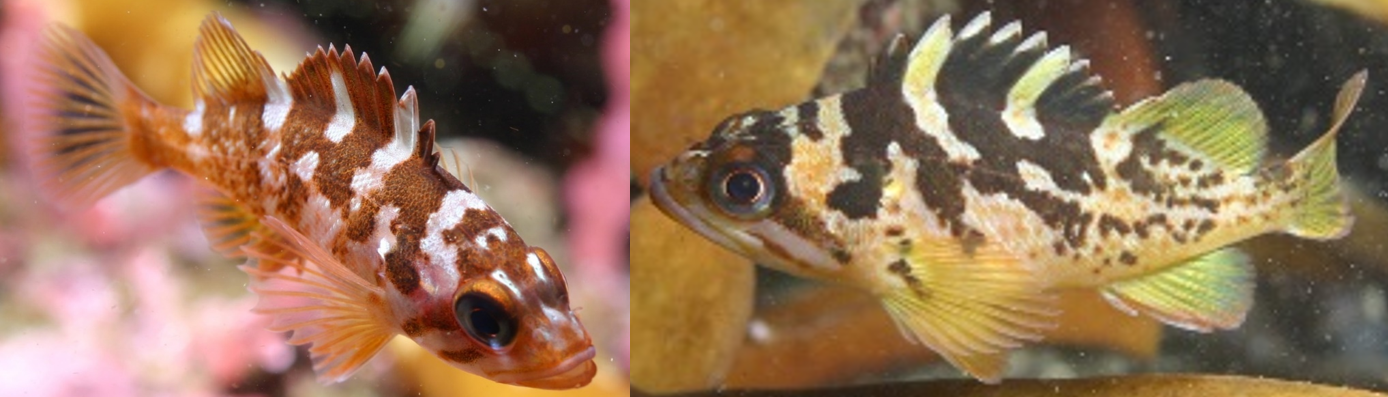
\includegraphics{cover_photo}~\\[1cm]
\pdftooltip{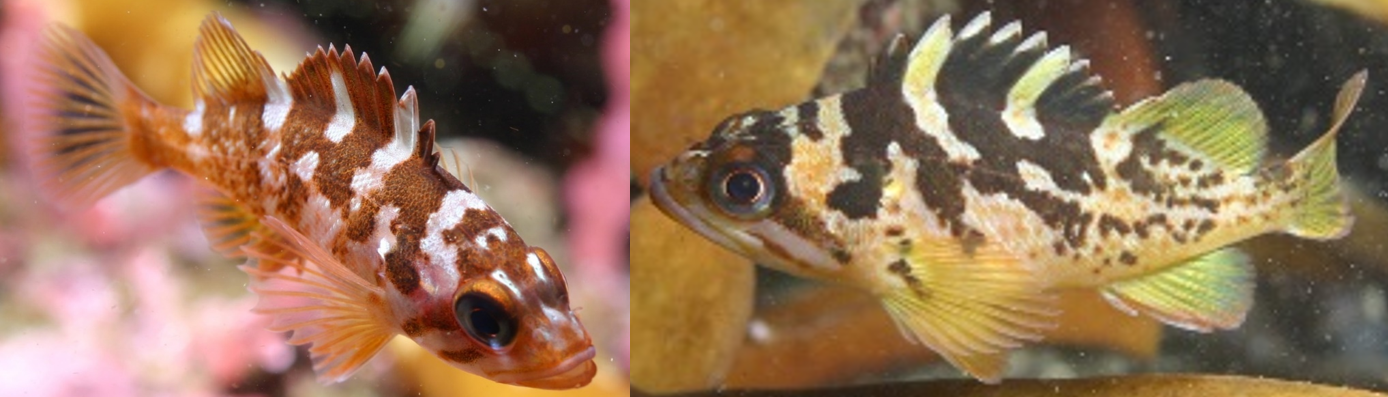
\includegraphics{cover_photo}}{This is a fish.}
Gopher rockfish (left) and black-and-yellow rockfish (right).      
\small
Photos by Steve Lonhart.

\vspace{.3cm}


Melissa H. Monk\textsuperscript{1}\\
Xi He\textsuperscript{1}\\

\vspace{.5cm}

\small
\textsuperscript{1}Southwest Fisheries Science Center, U.S. Department of Commerce, National Oceanic and Atmospheric Administration, National Marine Fisheries Service, 110 McAllister Way, Santa Cruz, California 95060\\

\vspace{1.5cm}


%\vfill
DRAFT SAFE\\
Disclaimer: This information is distributed solely for the purpose of pre-dissemination
peer review under applicable information quality guidelines. It has not been formally
disseminated by NOAA Fisheries. It does not represent and should not be construed to
represent any agency determination or policy. 

\vspace{.1cm}
%Bottom of the page
{\large \today}


\newpage{\thispagestyle{empty}}


\begin{flushleft}
This report may be cited as:

Monk, M. H.  and X. He. 2019. The Combined Status of Gopher \emph{Sebastes carnatus} and Black-and-Yellow Rockfishes \emph{Sebastes chrysomelas} in U.S. Waters Off California in 2019. Pacific Fishery Management Council, Portland, OR. Available from http://www.pcouncil.org/groundfish/stock-assessments/
\end{flushleft}

\maketitle

\pagenumbering{roman}
\setcounter{page}{1}
\end{center}

{
\setcounter{tocdepth}{4}
\tableofcontents
}
\setlength{\parskip}{5mm plus1mm minus1mm} \pagebreak

\setcounter{page}{1} \renewcommand{\thefigure}{\alph{figure}}
\renewcommand{\thetable}{\alph{table}}

\section*{Executive Summary}\label{executive-summary}
\addcontentsline{toc}{section}{Executive Summary}

\subsection*{Stock}\label{stock}
\addcontentsline{toc}{subsection}{Stock}

This assessment reports the status of the GBYR
(\emph{Sebastes carnatus/Sebastes chrysomelas}) resource in U.S. waters
off the coast of \ldots{} using data through 2018.

\subsection*{Catches}\label{catches}
\addcontentsline{toc}{subsection}{Catches}

Information on historical landings of GBYR are available back to
xxxx\ldots{} (Table \ref{tab:Exec_catch}). Commercial landings were
small during the years of World War II, ranging between 4 to 28 metric
tons (mt) per year.

(Figures \ref{fig:Exec_catch1}-\ref{fig:Exec_catch2})\\
(Figure \ref{fig:r4ss_catches})

Since 2000, annual total landings of GBYR have ranged between 70-169 mt,
with landings in 2018 totaling 92 mt.

\FloatBarrier

\begin{figure}
\centering
\includegraphics{Figures/rec_exec.png}
\caption{Catch history of GBYR for the recreational fleet.
\label{fig:Exec_catch1}}
\end{figure}

\begin{figure}
\centering
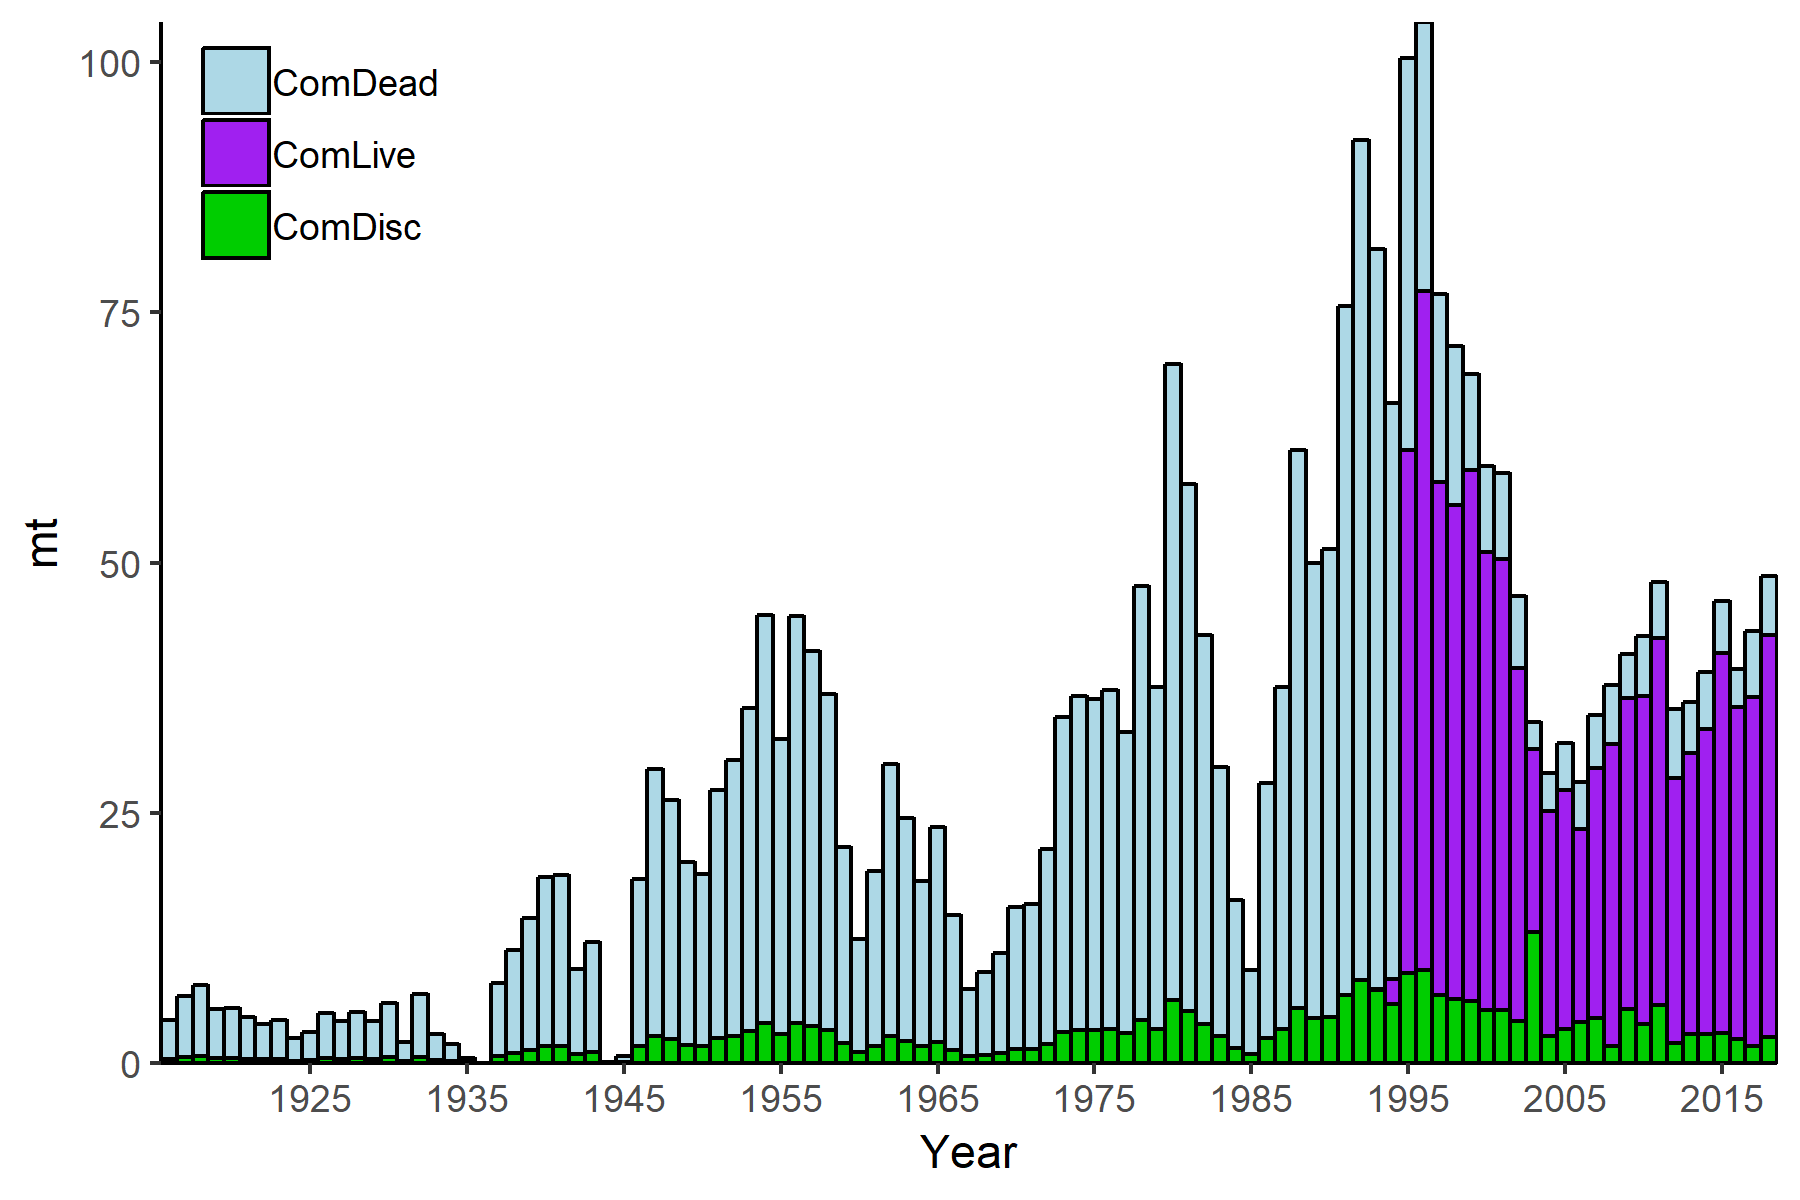
\includegraphics{Figures/comm_exec.png}
\caption{Catch history of GBYR for the commercial fleet by dead and live
landings, and discards. Catches in 1936 and 1946 were minimal.
\label{fig:Exec_catch2}}
\end{figure}

\FloatBarrier

\begin{figure}
\centering
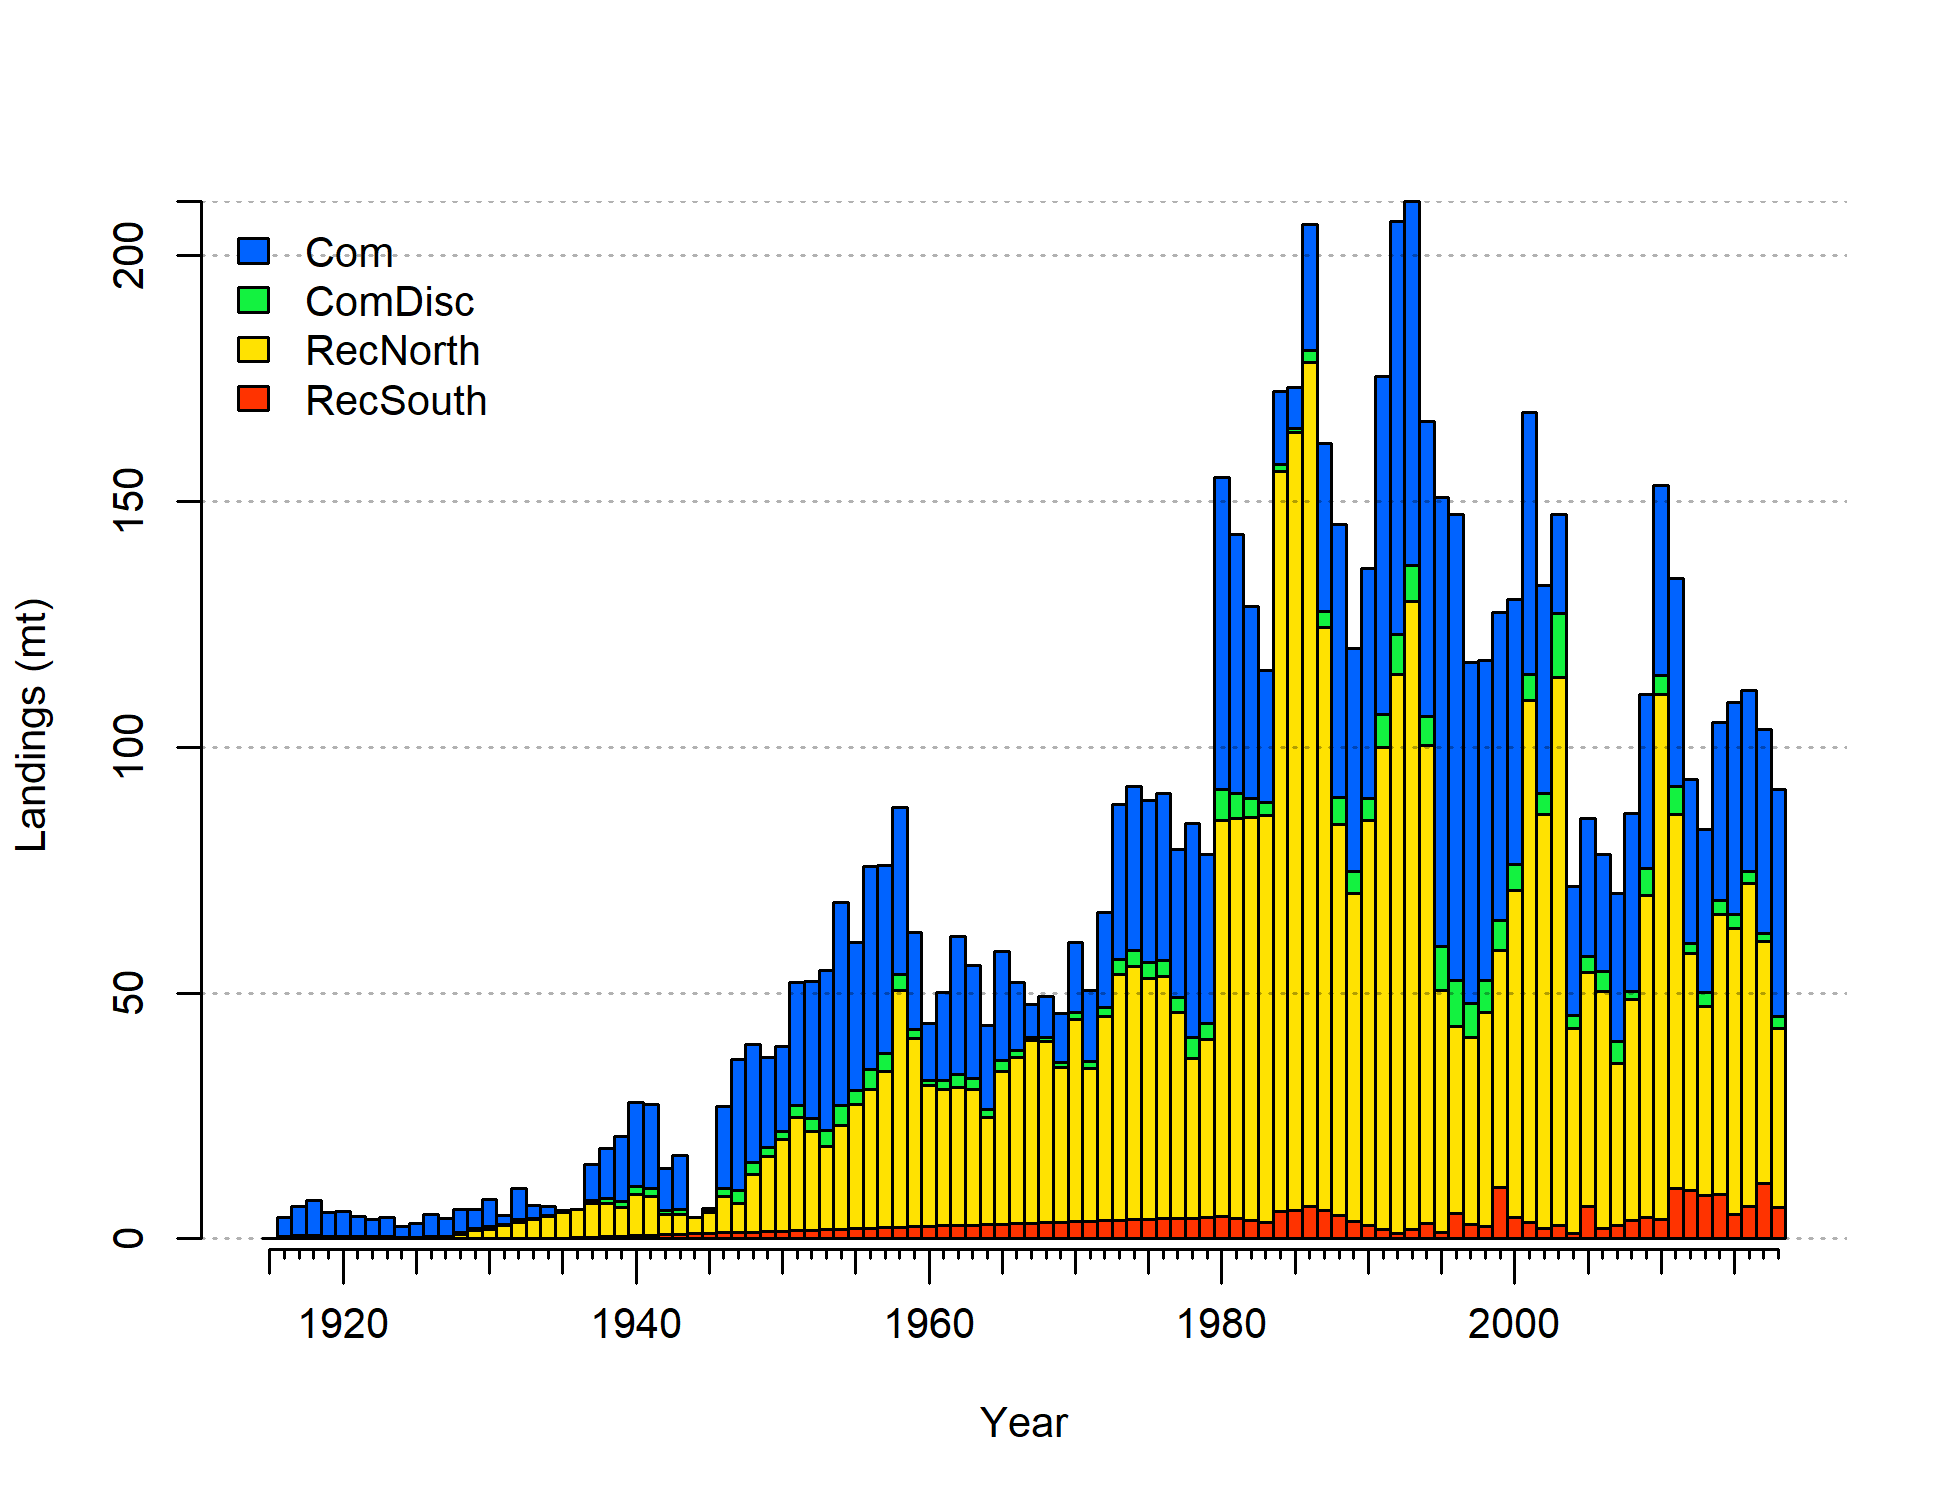
\includegraphics{r4ss/plots_mod1/catch2 landings stacked.png}
\caption{Catch history of GBYR in the model. \label{fig:r4ss_catches}}
\end{figure}

\begin{table}[ht]
\centering
\caption{Recent GBYR landings (mt) by 
                                            fleet.} 
\label{tab:Exec_catch}
\begin{tabular}{l>{\centering}p{1in}>{\centering}p{1in}>{\centering}p{1in}>{\centering}p{.9in}>{\centering}p{.9in}}
  \hline
Year & Commercial Retained & Commercial Discard & Recreational North & Recreational South & Total \\ 
  \hline
2009 & 35.62 & 5.38 & 65.64 & 4.30 & 110.93 \\ 
  2010 & 38.83 & 3.92 & 106.76 & 3.90 & 153.41 \\ 
  2011 & 42.39 & 5.72 & 76.16 & 10.24 & 134.52 \\ 
  2012 & 33.55 & 1.93 & 48.25 & 9.89 & 93.62 \\ 
  2013 & 33.45 & 2.85 & 38.43 & 8.86 & 83.59 \\ 
  2014 & 36.40 & 2.85 & 56.96 & 9.06 & 105.27 \\ 
  2015 & 43.25 & 2.93 & 58.09 & 5.00 & 109.27 \\ 
  2016 & 36.96 & 2.42 & 65.72 & 6.57 & 111.67 \\ 
  2017 & 42.04 & 1.65 & 49.36 & 11.15 & 104.19 \\ 
  2018 & 47.00 & 2.54 & 36.48 & 6.30 & 92.32 \\ 
   \hline
\end{tabular}
\end{table}

\FloatBarrier

\newpage

\subsection*{Data and Assessment}\label{data-and-assessment}
\addcontentsline{toc}{subsection}{Data and Assessment}

This a new full assessment for GBYR, which was last assessed in \ldots{}
using Stock Synthesis Version xx. This assessment uses the newest
version of Stock Synthesis (3.30.xx). The model begins in 1916, and
assumes the stock was at an unfished equilibrium that year.

(Figure \ref{fig:assess_region_map}).

\begin{figure}
\centering
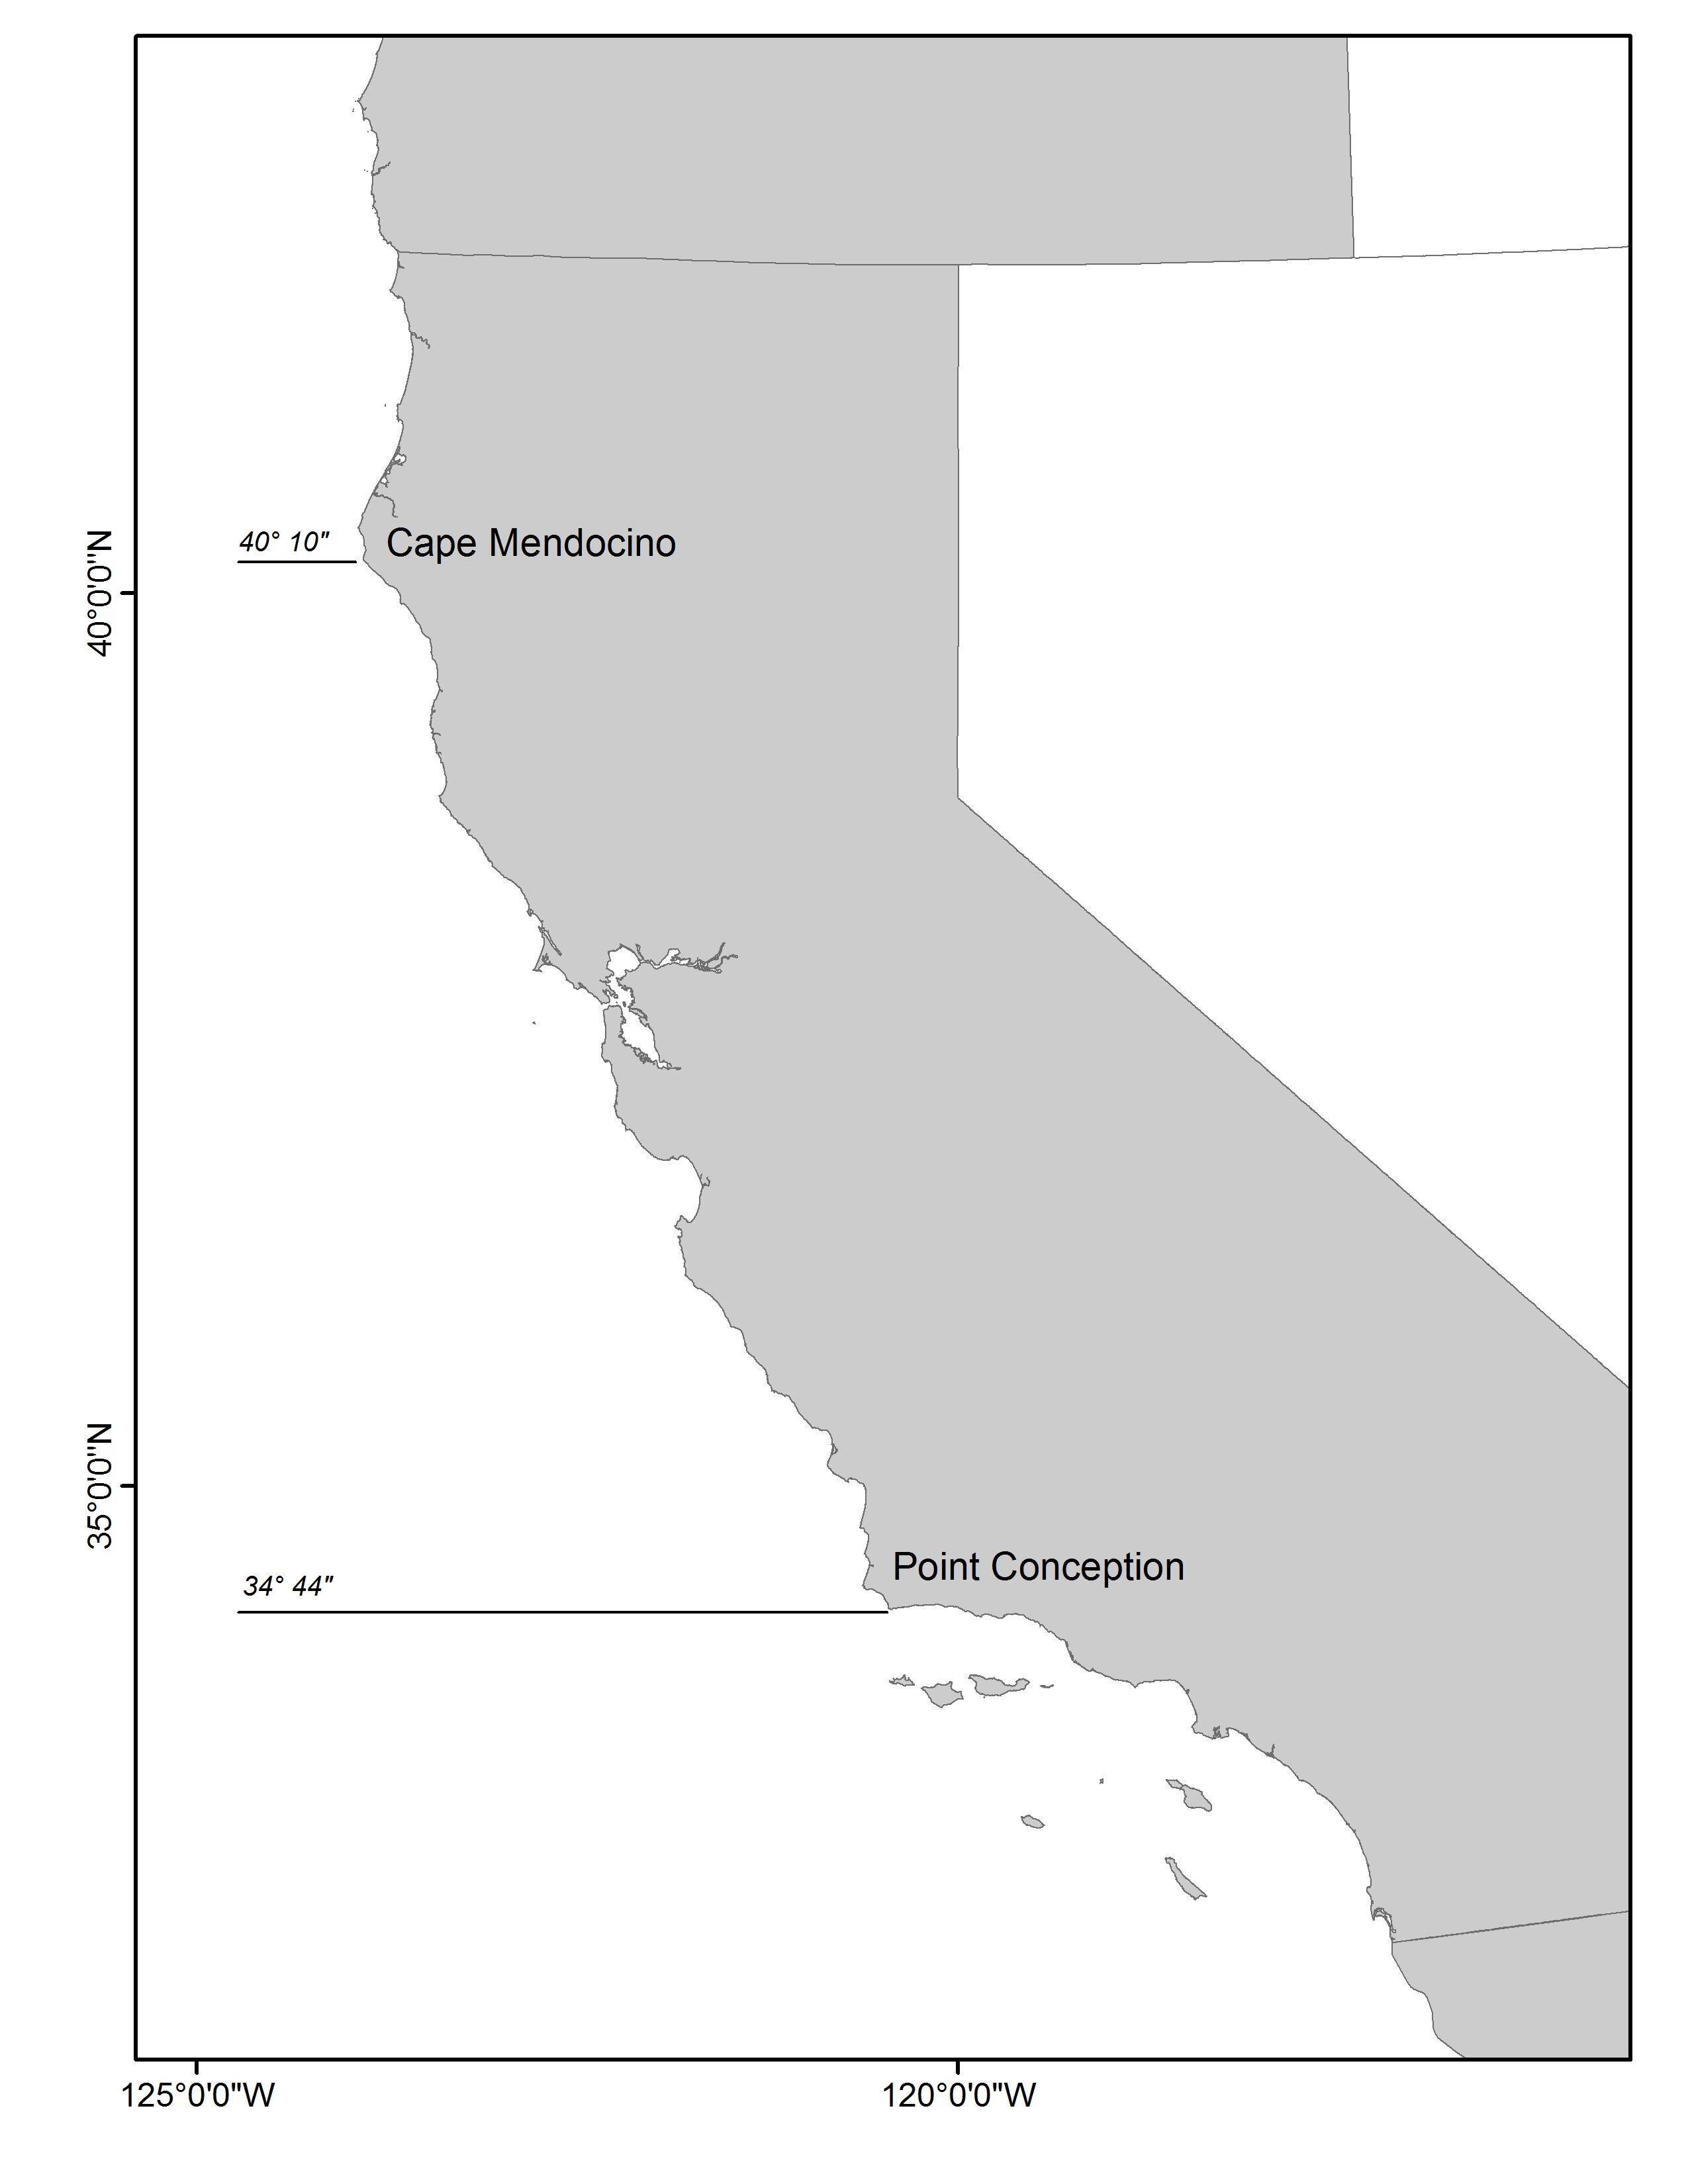
\includegraphics{Figures/assess_region_map.png}
\caption{Map depicting the core distribution of gopher and
black-and-yellow rockfishes. The stock assessment is bounded at Cape
Mendocino in the north to the U.S./Mexico border in the south.
\label{fig:assess_region_map}}
\end{figure}

\FloatBarrier

\subsection*{Stock Biomass}\label{stock-biomass}
\addcontentsline{toc}{subsection}{Stock Biomass}

(Figure \ref{fig:Spawnbio_all} and Table
\ref{tab:SpawningDeplete_mod1}).

The 2018 estimated spawning biomass relative to unfished equilibrium
spawning biomass is above the target of 40\% of unfished spawning
biomass at 4 520\% (95\% asymptotic interval: \(\pm\) 3 000\% - 6 050\%)
(Figure \ref{fig:RelDeplete_all}). Approximate confidence intervals
based on the asymptotic variance estimates show that the uncertainty in
the estimated spawning biomass is high.

\FloatBarrier

\begin{table}[ht]
\centering
\caption{Recent trend in beginning of the 
                                      year spawning output and depletion for
                                      the model for GBYR.} 
\label{tab:SpawningDeplete_mod1}
\begin{tabular}{l>{\centering}p{1.3in}>{\centering}p{1.2in}>{\centering}p{1in}>{\centering}p{1.2in}}
  \hline
Year & Spawning Output (million eggs) & \~{} 95\% confidence interval & Estimated depletion & \~{} 95\% confidence interval \\ 
  \hline
2010 & 834 & 520 - 1149 & 63.32 & 45.47 - 81.16 \\ 
  2011 & 764 & 469 - 1060 & 58.03 & 41.45 - 74.61 \\ 
  2012 & 707 & 429 - 985 & 53.69 & 38.2 - 69.18 \\ 
  2013 & 676 & 410 - 942 & 51.33 & 36.74 - 65.91 \\ 
  2014 & 654 & 397 - 911 & 49.64 & 35.74 - 63.55 \\ 
  2015 & 625 & 374 - 877 & 47.48 & 33.95 - 61.01 \\ 
  2016 & 602 & 352 - 852 & 45.71 & 32.24 - 59.18 \\ 
  2017 & 585 & 332 - 838 & 44.41 & 30.69 - 58.12 \\ 
  2018 & 580 & 320 - 841 & 44.06 & 29.81 - 58.32 \\ 
  2019 & 596 & 320 - 872 & 45.25 & 29.99 - 60.5 \\ 
   \hline
\end{tabular}
\end{table}

\FloatBarrier

\begin{figure}
\centering
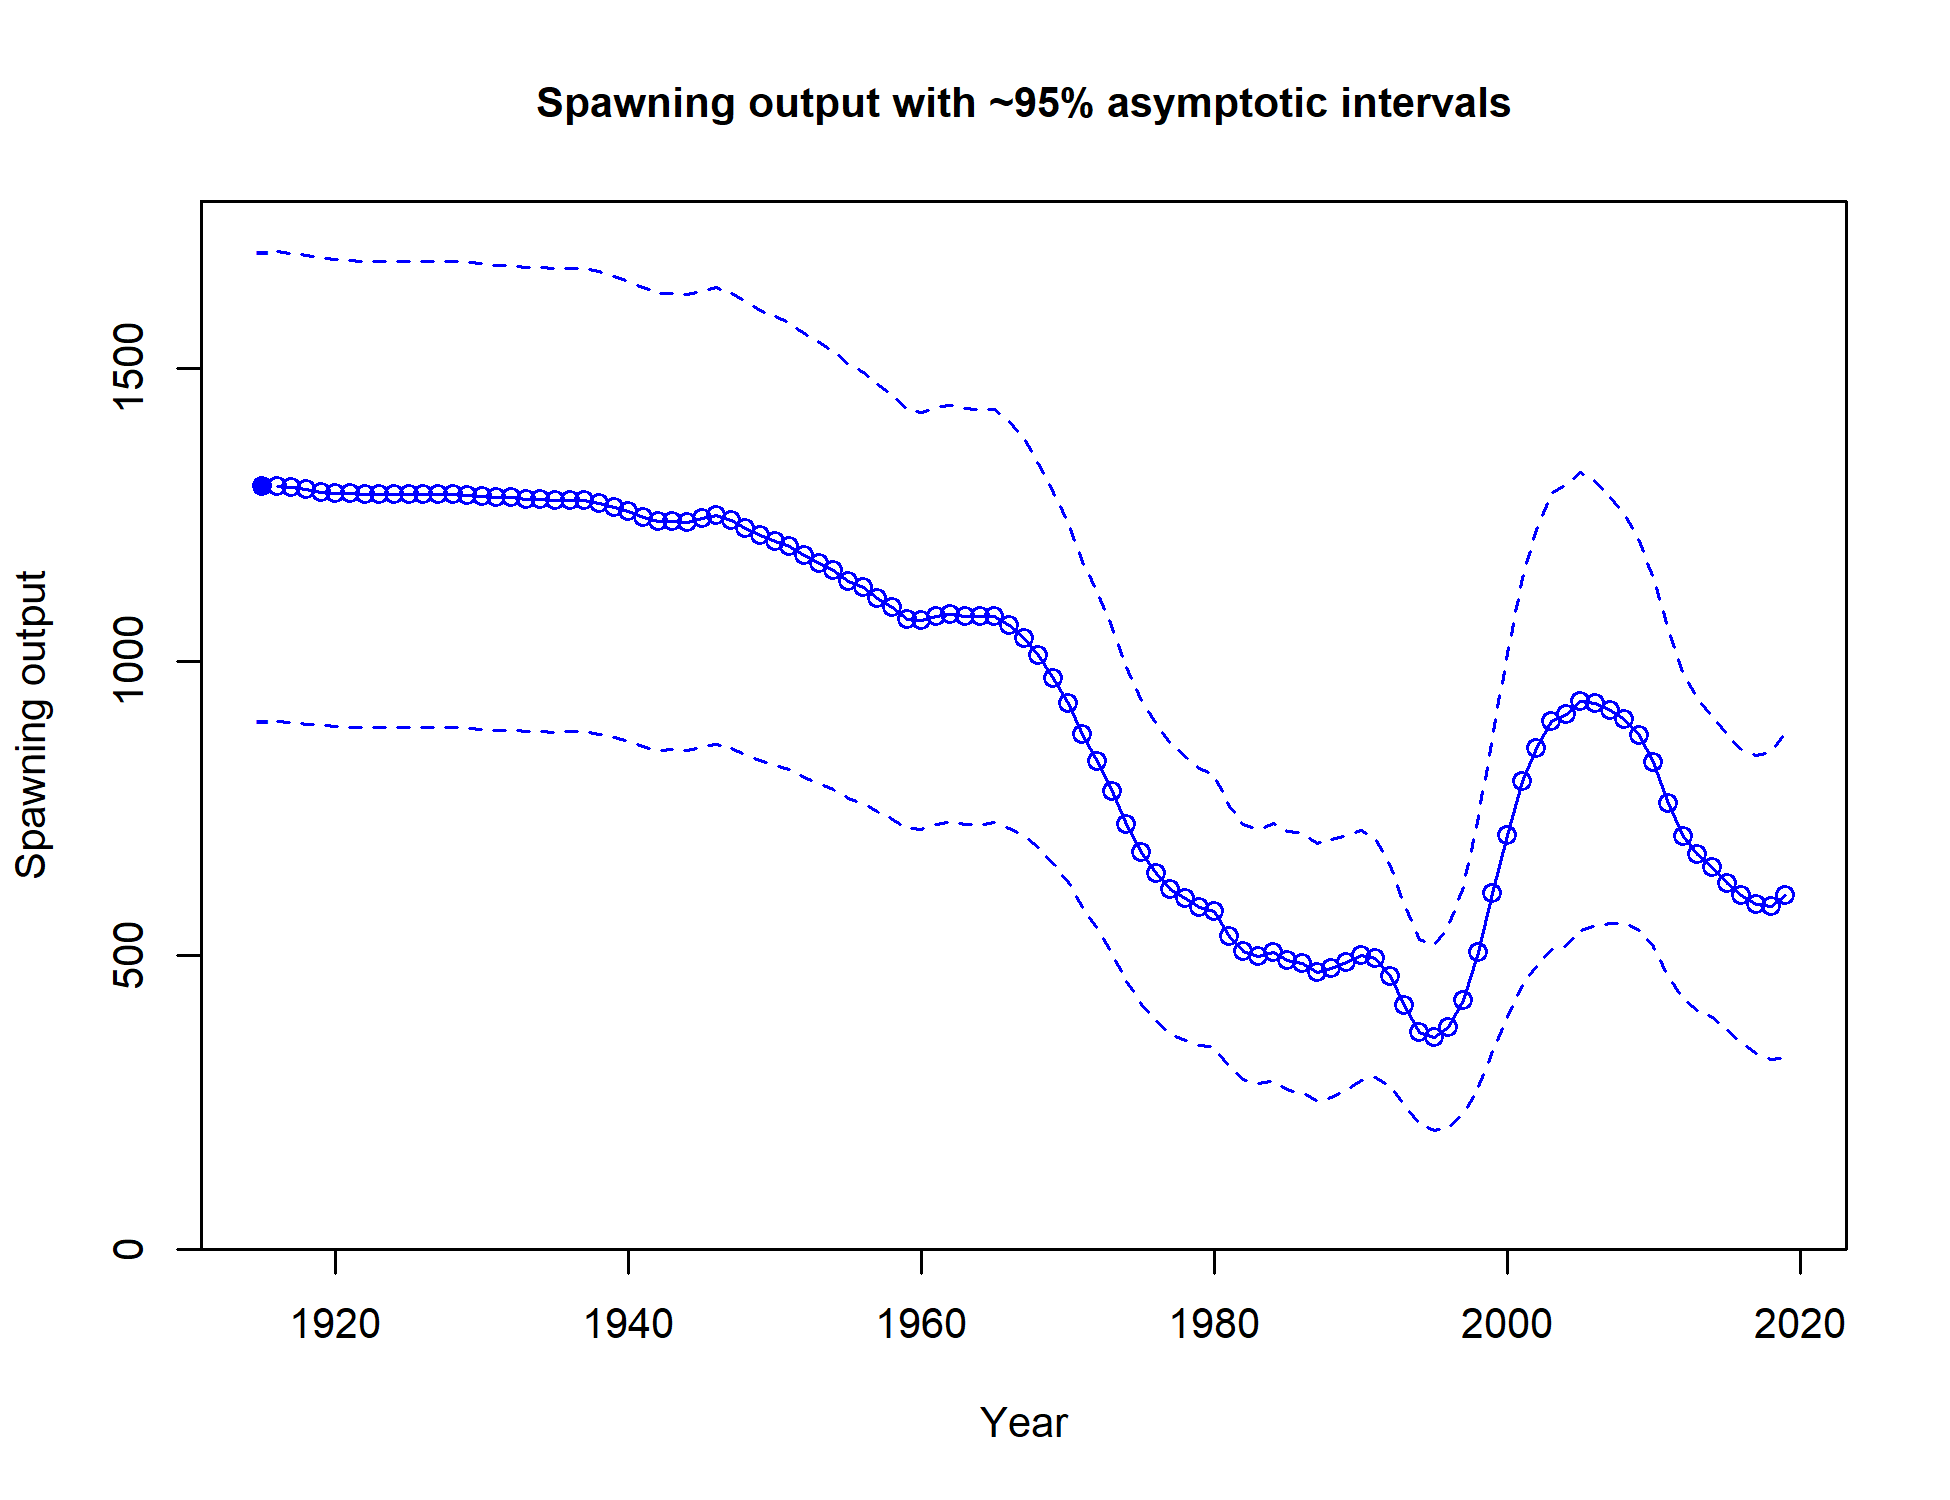
\includegraphics{r4ss/plots_mod1/ts7_Spawning_output_with_95_asymptotic_intervals_intervals.png}
\caption{Time series of spawning biomass trajectory (circles and line:
median; light broken lines: 95\% credibility intervals) for the base
case assessment model. \label{fig:Spawnbio_all}}
\end{figure}

\begin{figure}
\centering
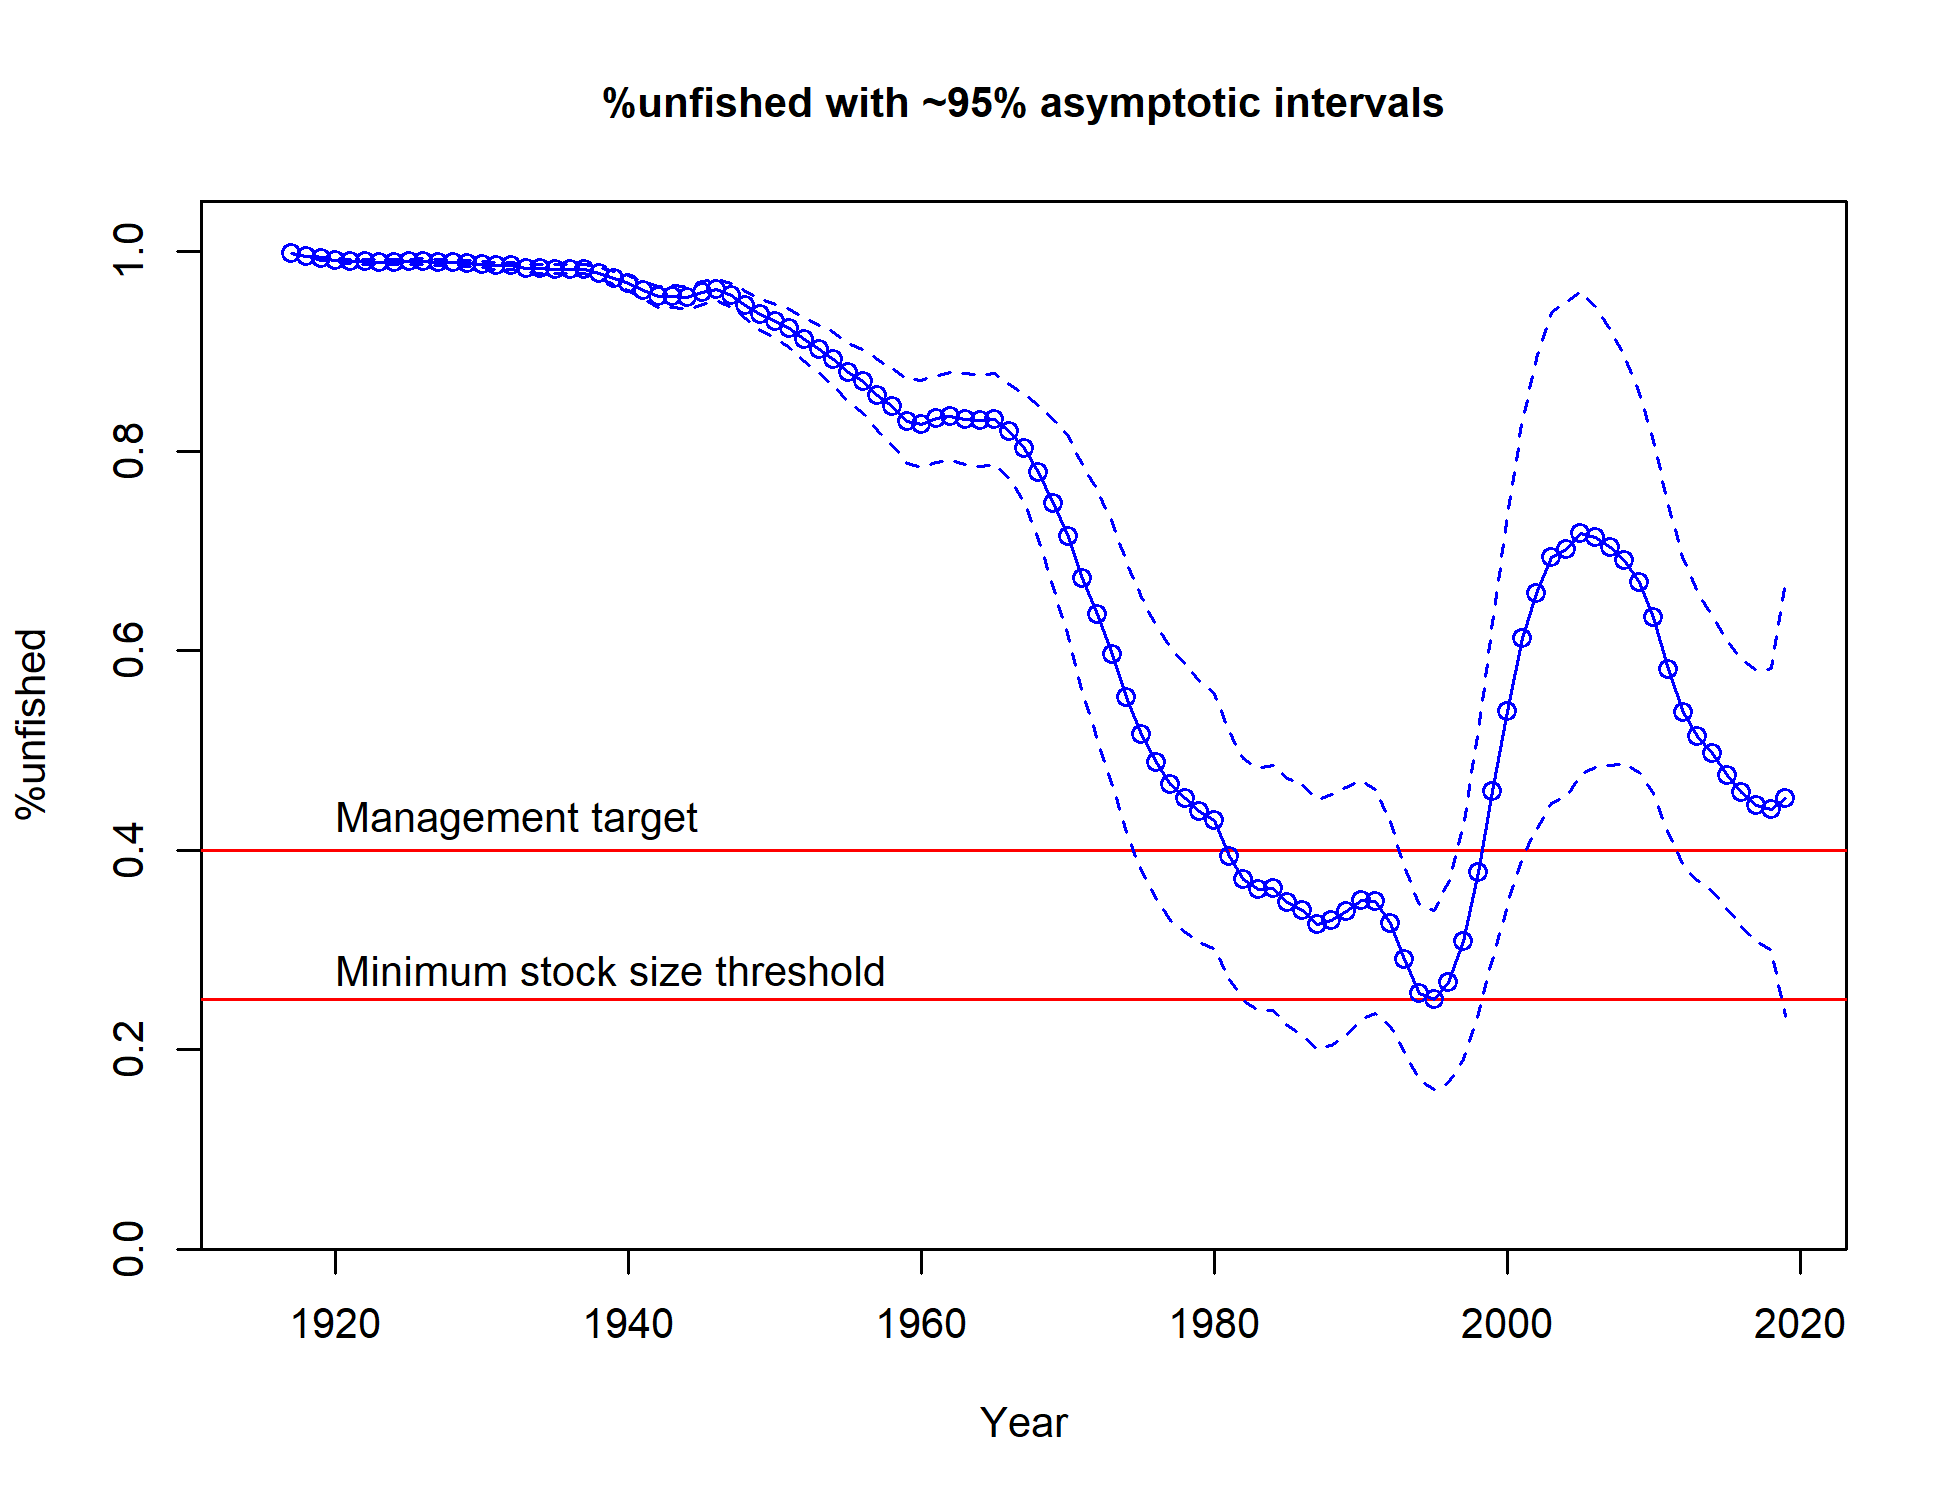
\includegraphics{r4ss/plots_mod1/ts9_unfished_with_95_asymptotic_intervals_intervals.png}
\caption{Estimated percent depletion with approximate 95\% asymptotic
confidence intervals (dashed lines) for the base case assessment model.
\label{fig:RelDeplete_all}}
\end{figure}

\FloatBarrier

\subsection*{Recruitment}\label{recruitment}
\addcontentsline{toc}{subsection}{Recruitment}

Recruitment deviations were estimated from xxxx-xxxx (Figure
\ref{fig:Recruits_all} and Table \ref{tab:Recruit_mod1}).

\begin{table}[ht]
\centering
\caption{Recent recruitment for the GBYR assessment.} 
\label{tab:Recruit_mod1}
\begin{tabular}{>{\centering}p{.8in}>{\centering}p{1.6in}>{\centering}p{1.6in}}
  \hline
Year & Estimated Recruitment (1,000s) & \~{} 95\% confidence interval \\ 
  \hline
2010 & 3680 & 1452 - 9327 \\ 
  2011 & 3319 & 1277 - 8625 \\ 
  2012 & 3393 & 1279 - 9001 \\ 
  2013 & 4194 & 1580 - 11131 \\ 
  2014 & 6319 & 2385 - 16738 \\ 
  2015 & 8445 & 3154 - 22610 \\ 
  2016 & 6941 & 2564 - 18788 \\ 
  2017 & 5137 & 1845 - 14301 \\ 
  2018 & 4177 & 1469 - 11875 \\ 
  2019 & 4276 & 1486 - 12305 \\ 
   \hline
\end{tabular}
\end{table}

\FloatBarrier

\begin{figure}
\centering
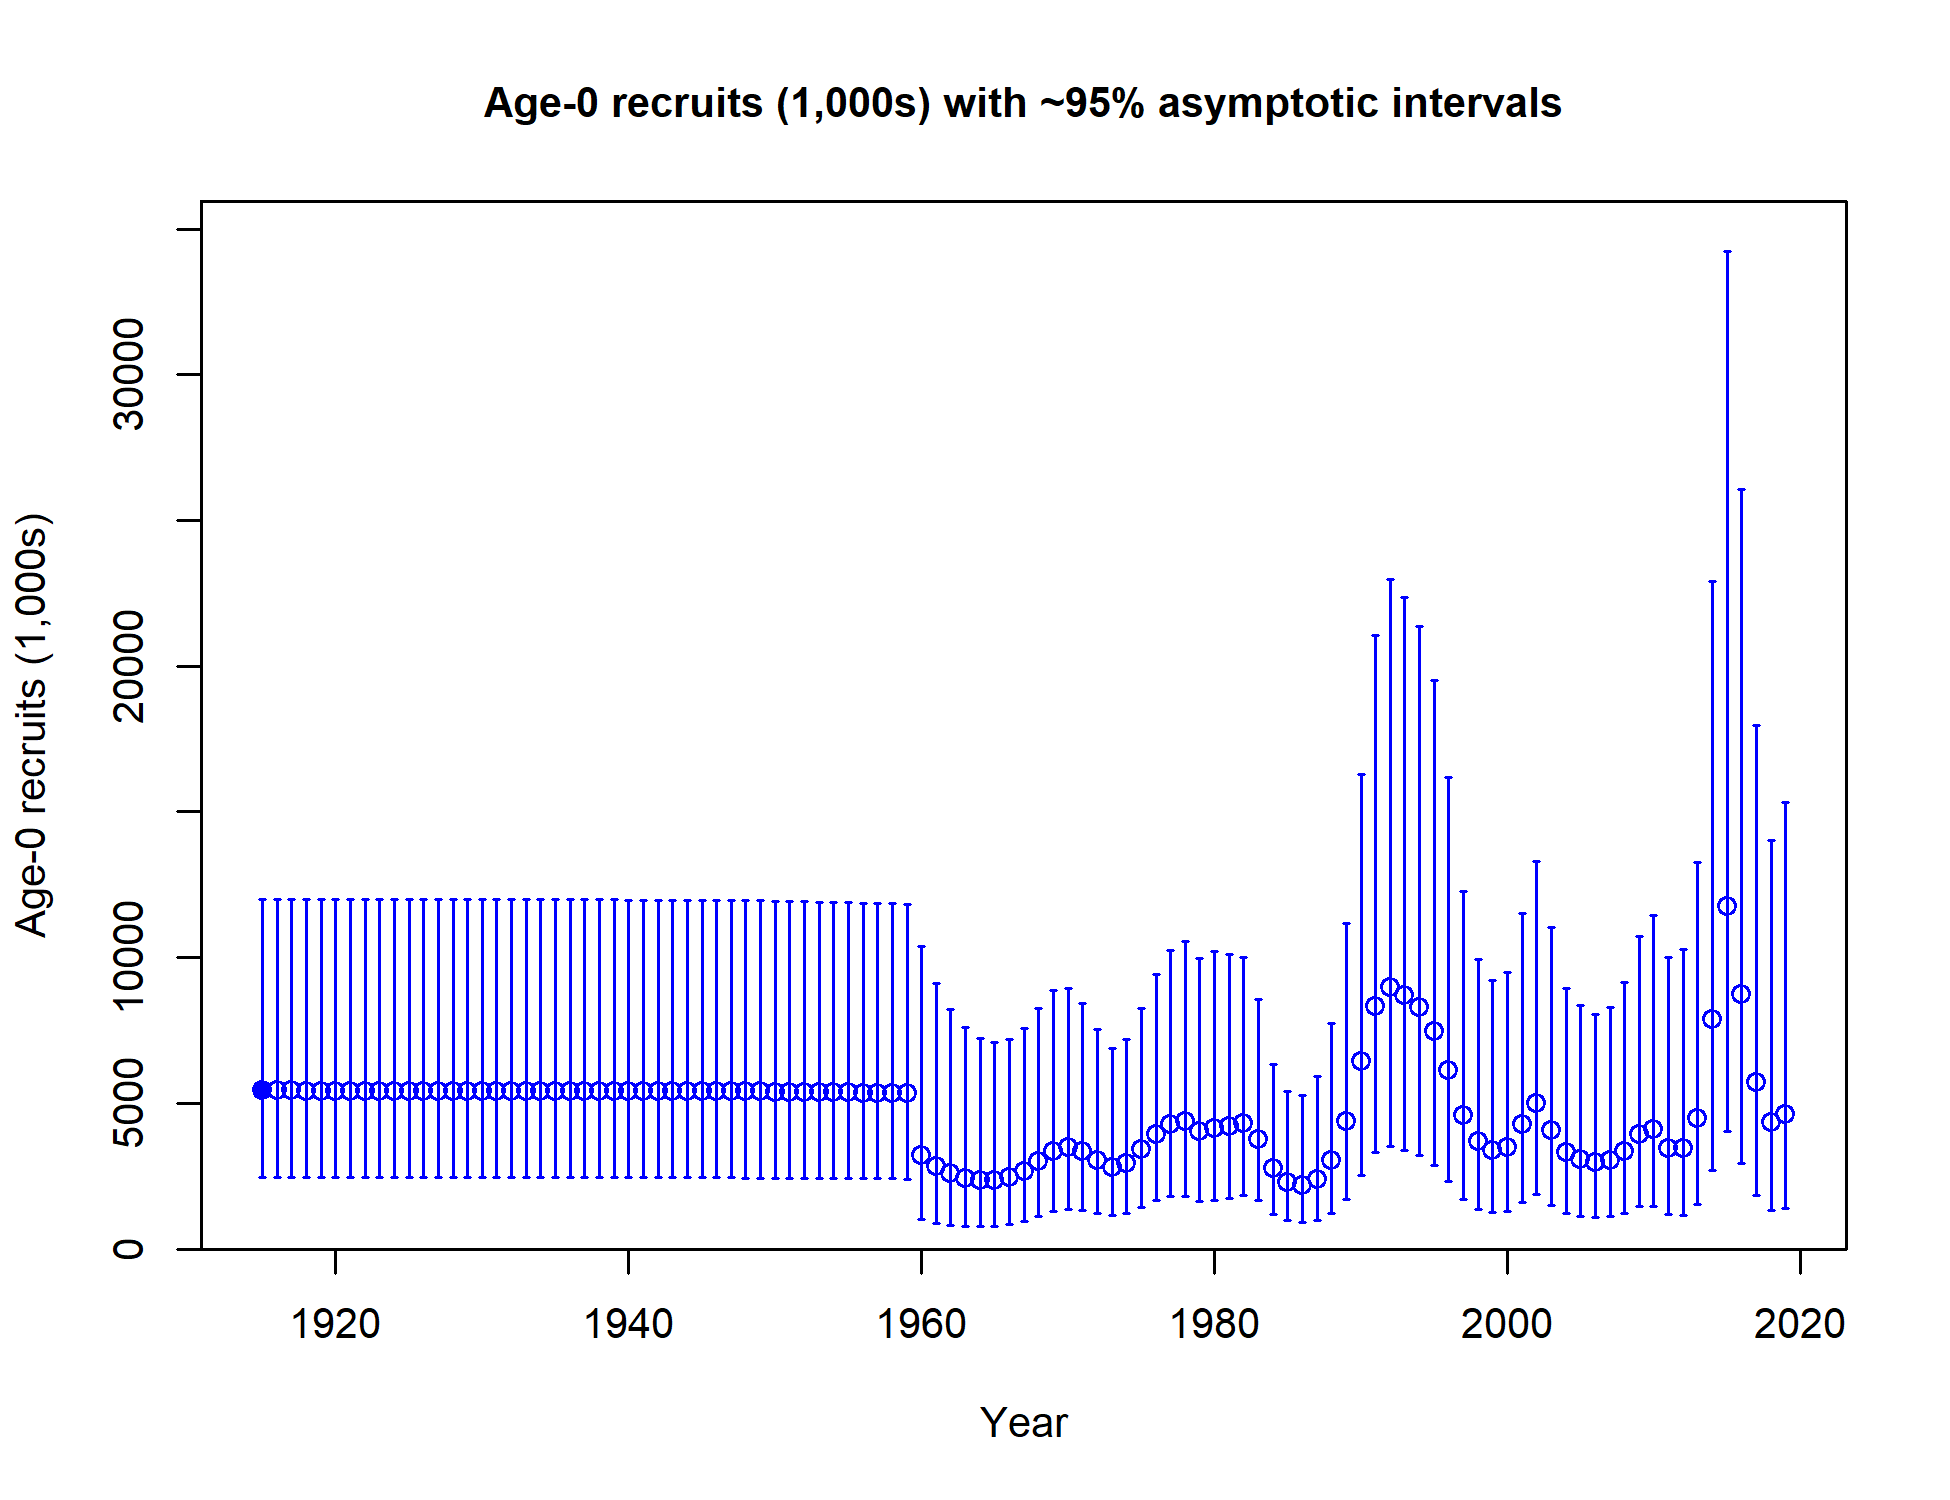
\includegraphics{r4ss/plots_mod1/ts11_Age-0_recruits_(1000s)_with_95_asymptotic_intervals.png}
\caption{Time series of estimated GBYR recruitments for the base-case
model with 95\% confidence or credibility intervals.
\label{fig:Recruits_all}}
\end{figure}

\FloatBarrier

\subsection*{Exploitation status}\label{exploitation-status}
\addcontentsline{toc}{subsection}{Exploitation status}

Harvest rates estimated by the base model \ldots{}.. management target
levels (Table \ref{tab:SPR_Exploit_mod1} and Figure \ref{fig:SPR_all}).

\FloatBarrier

\begin{table}[ht]
\centering
\caption{Recent trend in spawning potential 
                                        ratio and exploitation for GBYR in the model.  Fishing intensity is (1-SPR) 
                                        divided by 50\% (the SPR target) and exploitation 
                                        is F divided by F\textsubscript{SPR}.} 
\label{tab:SPR_Exploit_mod1}
\begin{tabular}{l>{\centering}p{1in}>{\centering}p{1.2in}>{\centering}p{1in}>{\centering}p{1.2in}}
  \hline
Year & Fishing intensity & \~{} 95\% confidence interval & Exploitation rate & \~{} 95\% confidence interval \\ 
  \hline
2009 & 0.61 & 0.38 - 0.83 & 0.08 & 0.05 - 0.1 \\ 
  2010 & 0.74 & 0.5 - 0.99 & 0.11 & 0.07 - 0.15 \\ 
  2011 & 0.74 & 0.49 - 0.99 & 0.10 & 0.06 - 0.14 \\ 
  2012 & 0.63 & 0.4 - 0.87 & 0.08 & 0.05 - 0.1 \\ 
  2013 & 0.61 & 0.38 - 0.84 & 0.07 & 0.04 - 0.1 \\ 
  2014 & 0.71 & 0.46 - 0.96 & 0.09 & 0.05 - 0.12 \\ 
  2015 & 0.74 & 0.49 - 0.99 & 0.09 & 0.05 - 0.13 \\ 
  2016 & 0.77 & 0.51 - 1.04 & 0.09 & 0.05 - 0.13 \\ 
  2017 & 0.77 & 0.5 - 1.04 & 0.08 & 0.04 - 0.12 \\ 
  2018 & 0.73 & 0.46 - 1 & 0.07 & 0.03 - 0.1 \\ 
   \hline
\end{tabular}
\end{table}

\FloatBarrier

\begin{figure}
\centering
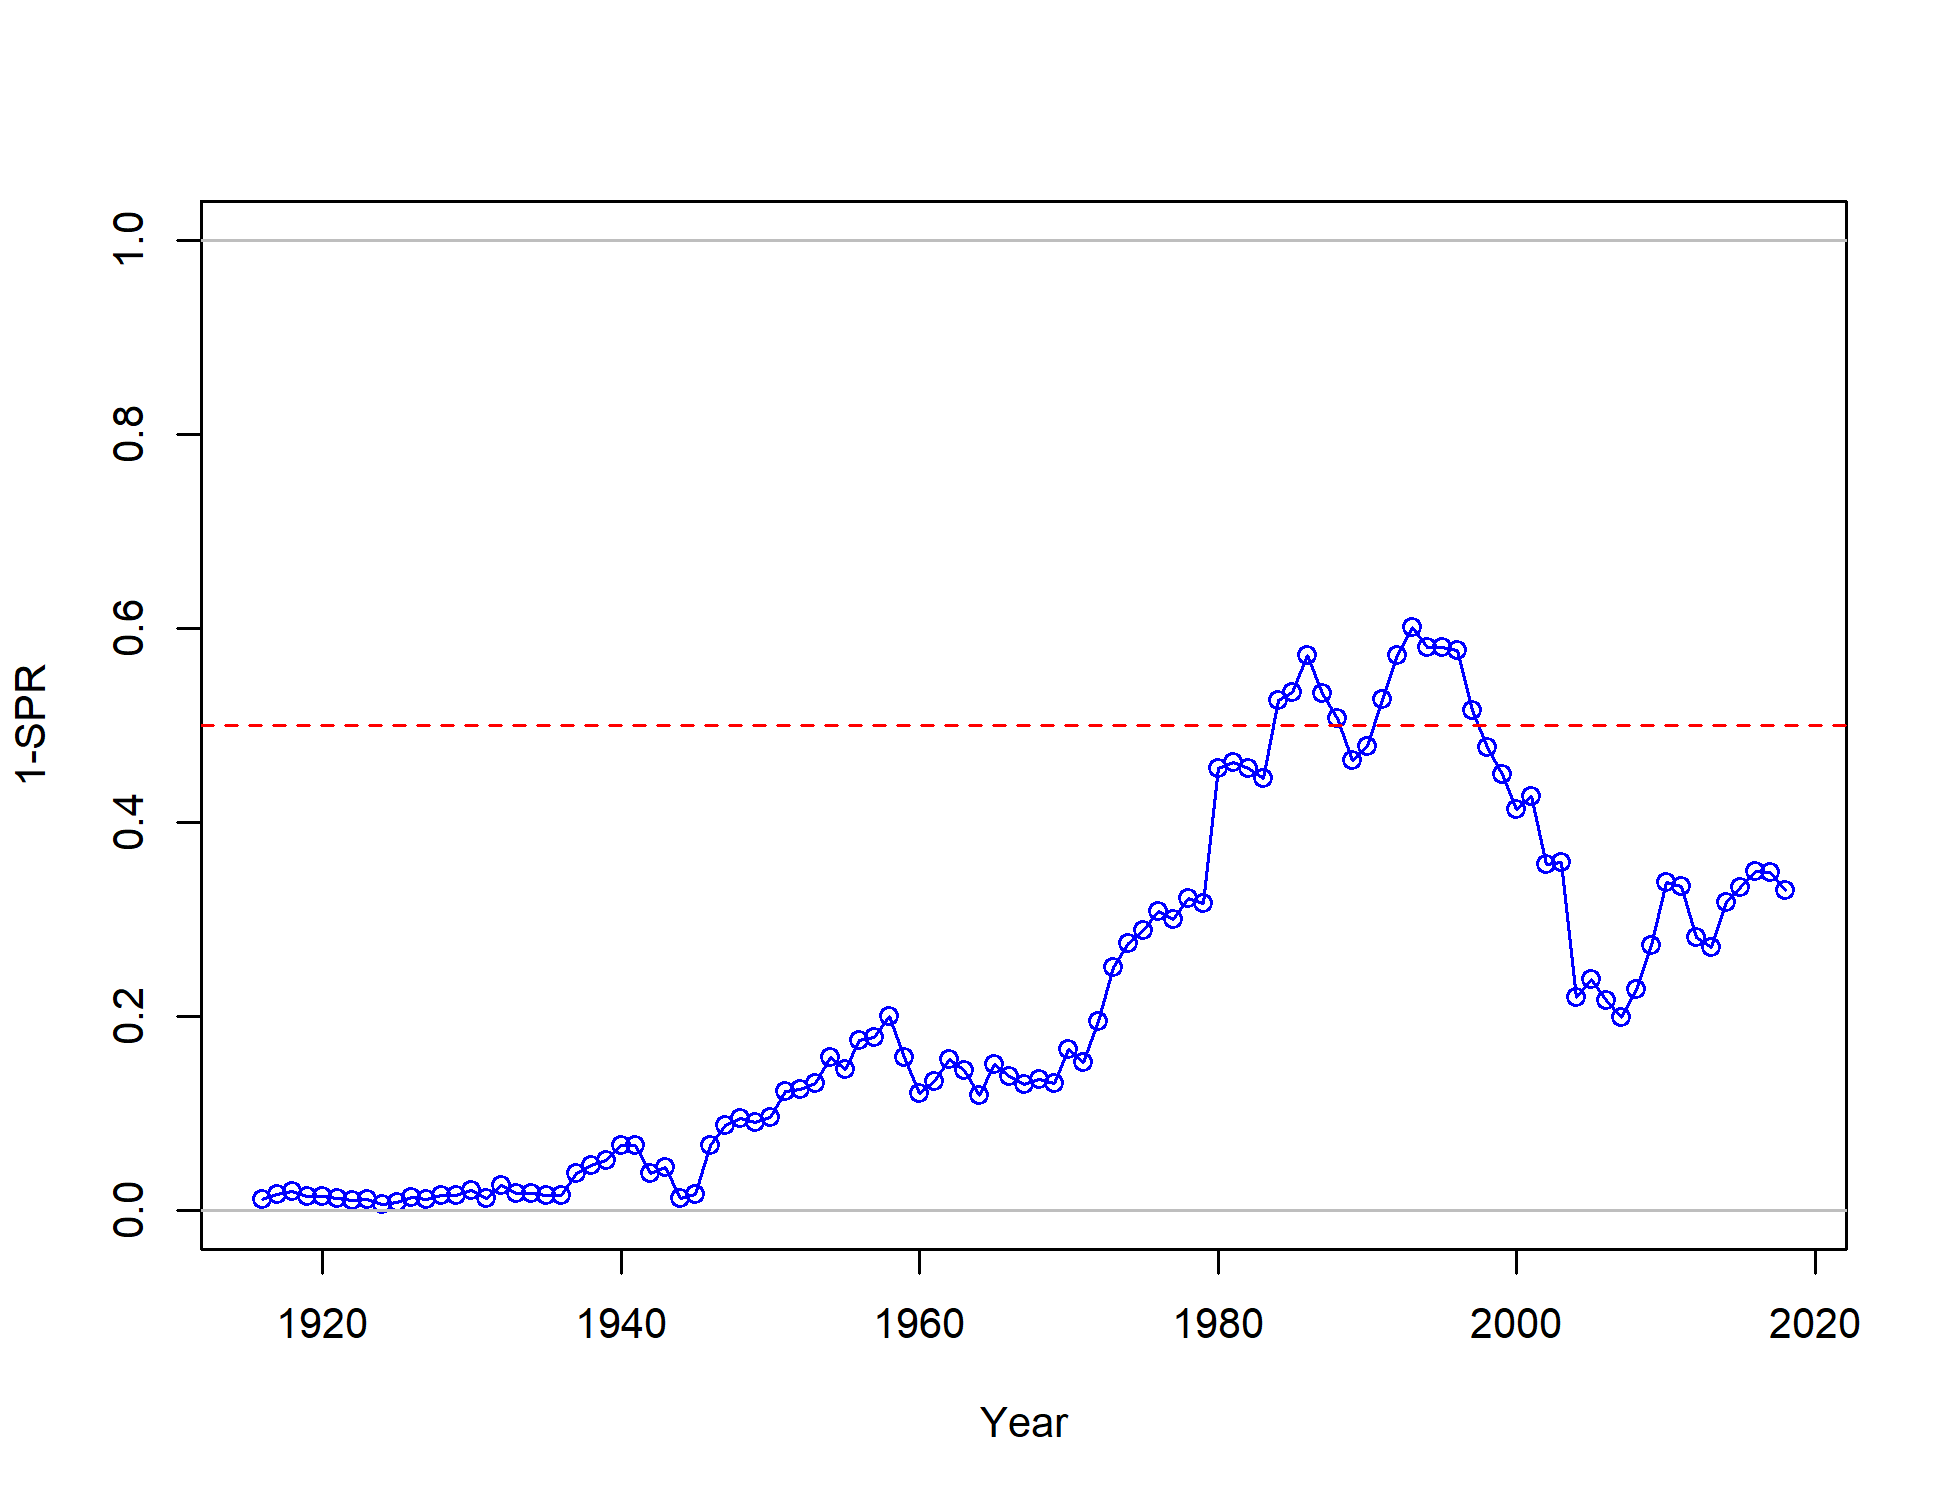
\includegraphics{r4ss/plots_mod1/SPR2_minusSPRseries.png}
\caption{Estimated spawning potential ratio (SPR) for the base-case
model. One minus SPR is plotted so that higher exploitation rates occur
on the upper portion of the y-axis. The management target is plotted as
a red horizontal line and values above this reflect harvests in excess
of the overfishing proxy based on the SPR\textsubscript{50\%} harvest
rate. The last year in the time series is 2018. \label{fig:SPR_all}}
\end{figure}

\FloatBarrier

\subsection*{Ecosystem Considerations}\label{ecosystem-considerations}
\addcontentsline{toc}{subsection}{Ecosystem Considerations}

In this assessment, ecosystem considerations were not explicitly
included in the analysis.\\
This is primarily due to a lack of relevant data and results of analyses
(conducted elsewhere) that could contribute ecosystem-related
quantitative information for the assessment.

\subsection*{Reference Points}\label{reference-points}
\addcontentsline{toc}{subsection}{Reference Points}

This stock assessment estimates that GBYR in the model is above the
biomass target (\(SB_{40\%}\)), and well above the minimum stock size
threshold (\(SB_{25\%}\)). The estimated relative depletion level for
the base model in 2019 is 4 520\% (95\% asymptotic interval: \(\pm\) 3
000\% - 6 050\%, corresponding to an unfished spawning biomass of 596
million eggs (95\% asymptotic interval: 320 - 872 million eggs) of
spawning biomass in the base model (Table \ref{tab:Ref_pts_mod1}).
Unfished age 1+ biomass was estimated to be 2,149 mt in the base case
model. The target spawning biomass (\(SB_{40\%}\)) is 527 million eggs,
which corresponds with an equilibrium yield of 179 mt. Equilibrium yield
at the proxy \(F_{MSY}\) harvest rate corresponding to \(SPR_{50\%}\) is
167 mt (Figure \ref{fig:Yield_all}).

\FloatBarrier

\begin{table}[ht]
\centering
\caption{Summary of reference 
                                      points and management quantities for the 
                                      base case model.} 
\label{tab:Ref_pts_mod1}
\begin{tabular}{>{\raggedright}p{4.1in}>{\raggedleft}p{.62in}>{\raggedleft}p{.62in}>{\raggedleft}p{.62in}}
  \hline
\textbf{Quantity} & \textbf{Estimate} & \textbf{Low 2.5\%  limit} & \textbf{High 2.5\%  limit} \\ 
  \hline
Unfished spawning output (million eggs) & 1,317 & 930 & 1,705 \\ 
  Unfished age 1+ biomass (mt) & 2,149 & 1,664 & 2,634 \\ 
  Unfished recruitment ($R_{0}$) & 4,784 & 1,164 & 8,404 \\ 
  Spawning output(2018 million eggs) & 580 & 320 & 841 \\ 
  Depletion (2018) & 0.441 & 0.298 & 0.583 \\ 
  \textbf{$\text{Reference points based on } \mathbf{SB_{40\%}}$} &  &  &  \\ 
  Proxy spawning output ($B_{40\%}$) & 527 & 428 & 626 \\ 
  SPR resulting in $B_{40\%}$ ($SPR_{B40\%}$) & 0.458 & 0.458 & 0.458 \\ 
  Exploitation rate resulting in $B_{40\%}$ & 0.151 & 0.107 & 0.195 \\ 
  Yield with $SPR_{B40\%}$ at $B_{40\%}$ (mt) & 179 & 108 & 251 \\ 
  \textbf{\textit{Reference points based on SPR proxy for MSY}} &  &  &  \\ 
  Spawning output & 588 & 477 & 698 \\ 
  $SPR_{proxy}$ & 0.5 &  &  \\ 
  Exploitation rate corresponding to $SPR_{proxy}$ & 0.131 & 0.094 & 0.169 \\ 
  Yield with $SPR_{proxy}$ at $SB_{SPR}$ (mt) & 167 & 101 & 233 \\ 
  \textbf{\textit{Reference points based on estimated MSY values}} &  &  &  \\ 
  Spawning output at $MSY$ ($SB_{MSY}$) & 279 & 226 & 333 \\ 
  $SPR_{MSY}$ & 0.289 & 0.278 & 0.299 \\ 
  Exploitation rate at $MSY$ & 0.266 & 0.194 & 0.339 \\ 
  Dead Catch $MSY$ (mt) & 210 & 121 & 299 \\ 
  Retained Catch $MSY$ (mt) & 210 & 121 & 299 \\ 
   \hline
\end{tabular}
\end{table}

\FloatBarrier

\subsection*{Management Performance}\label{management-performance}
\addcontentsline{toc}{subsection}{Management Performance}

Table \ref{tab:mnmgt_perform}

\begin{table}[ht]
\centering
\caption{Recent trend in total mortality for gopher and 
                            black-and-yellow rockfishes (GBYR), combined, relative to the 
                             management guidelines for the minor nearshore rockfish 
                             south of $40^\circ 10^\prime$ N. latitude. 
                             Total mortality estiamtes are based on annual reports 
                                from the NMFS NWFSC} 
\label{tab:mnmgt_perform}
\begin{tabular}{lllll}
  \hline
   \multicolumn{1}{c}{} & \multicolumn{1}{c}{GBYR} & \multicolumn{3}{c}{Minor Nearshore Rockfish} \\  \cmidrule(lr){2-2} \cmidrule(lr){3-5}
   \hline
Year & Total mortality & Total mortality & ACL & OFL \\ 
  \hline
\textbf{2011} & 122.87 & 436 & 1,001 & 1,156 \\ 
  \textbf{2012} & 91.96 & 445 & 1,001 & 1,145 \\ 
  \textbf{2013} & 104.53 & 495 & 990 & 1,164 \\ 
  \textbf{2014} & 103.63 & 596 & 990 & 1,160 \\ 
  \textbf{2015} & 107.95 & 676 & 1,114 & 1,313 \\ 
  \textbf{2016} & 111.55 & 641 & 1,006 & 1,288 \\ 
  \textbf{2017} & - & - & 1,329 & 1,163 \\ 
  \textbf{2018} & - & - & 1,344 & 1,179 \\ 
   \hline
   \hline
\end{tabular}
\end{table}

\subsection*{Unresolved Problems and Major
Uncertainties}\label{unresolved-problems-and-major-uncertainties}
\addcontentsline{toc}{subsection}{Unresolved Problems and Major
Uncertainties}

\FloatBarrier

\subsection*{Decision Table}\label{decision-table}
\addcontentsline{toc}{subsection}{Decision Table}

\begin{table}[ht]
\centering
\caption{Projections of potential OFL (mt) for 
                                        each model, using the base model forecast.} 
\label{tab:OFL_projection}
\begin{tabular}{lr}
  \hline
Year & OFL \\ 
  \hline
2019 & 180.21 \\ 
  2020 & 168.28 \\ 
  2021 & 167.05 \\ 
  2022 & 174.54 \\ 
  2023 & 187.31 \\ 
  2024 & 200.67 \\ 
  2025 & 210.28 \\ 
  2026 & 213.76 \\ 
  2027 & 211.19 \\ 
  2028 & 204.47 \\ 
  2029 & 196.15 \\ 
  2030 & 188.32 \\ 
   \hline
\end{tabular}
\end{table}\begin{table}[ht]
\centering
\caption{Summary of 10-year 
                                             projections beginning in 2020 
                                             for alternate states of nature based on 
                                             an axis of uncertainty for the model.  Columns range over low, mid, and high
                                             states of nature, and rows range over different 
                                             assumptions of catch levels. An entry of "--" 
                                             indicates that the stock is driven to very low 
                                             abundance under the particular scenario.} 
\label{tab:Decision_table_mod1}
\scalebox{0.85}{
\begin{tabular}{l|cc|>{\centering}p{.7in}c|>{\centering}p{.7in}c|>{\centering}p{.7in}c}
   \multicolumn{3}{c}{}  &  \multicolumn{2}{c}{} 
                               & \multicolumn{2}{c}{\textbf{States of nature}} 
                               & \multicolumn{2}{c}{} \\
  \multicolumn{3}{c}{}  &  \multicolumn{2}{c}{Low M 0.05} 
                               & \multicolumn{2}{c}{Base M 0.07} 
                               &  \multicolumn{2}{c}{High M 0.09} \\
 \hline
 & Year & Catch & Spawning Output & Depletion & Spawning Output & Depletion & Spawning Output & Depletion \\ 
  \hline
 & 2019 & - & - & - & - & - & - & - \\ 
   & 2020 & - & - & - & - & - & - & - \\ 
   & 2021 & - & - & - & - & - & - & - \\ 
  40-10 Rule,  & 2022 & - & - & - & - & - & - & - \\ 
  Low M & 2023 & - & - & - & - & - & - & - \\ 
   & 2024 & - & - & - & - & - & - & - \\ 
   & 2025 & - & - & - & - & - & - & - \\ 
   & 2026 & - & - & - & - & - & - & - \\ 
   & 2027 & - & - & - & - & - & - & - \\ 
   & 2028 & - & - & - & - & - & - & - \\ 
   \hline
 & 2019 & - & - & - & - & - & - & - \\ 
   & 2020 & - & - & - & - & - & - & - \\ 
   & 2021 & - & - & - & - & - & - & - \\ 
  40-10 Rule & 2022 & - & - & - & - & - & - & - \\ 
   & 2023 & - & - & - & - & - & - & - \\ 
   & 2024 & - & - & - & - & - & - & - \\ 
   & 2025 & - & - & - & - & - & - & - \\ 
   & 2026 & - & - & - & - & - & - & - \\ 
   & 2027 & - & - & - & - & - & - & - \\ 
   & 2028 & - & - & - & - & - & - & - \\ 
   \hline
 & 2019 & - & - & - & - & - & - & - \\ 
   & 2020 & - & - & - & - & - & - & - \\ 
   & 2021 & - & - & - & - & - & - & - \\ 
  40-10 Rule, & 2022 & - & - & - & - & - & - & - \\ 
  High M & 2023 & - & - & - & - & - & - & - \\ 
   & 2024 & - & - & - & - & - & - & - \\ 
   & 2025 & - & - & - & - & - & - & - \\ 
   & 2026 & - & - & - & - & - & - & - \\ 
   & 2027 & - & - & - & - & - & - & - \\ 
   & 2028 & - & - & - & - & - & - & - \\ 
   \hline
 & 2019 & - & - & - & - & - & - & - \\ 
   & 2020 & - & - & - & - & - & - & - \\ 
   & 2021 & - & - & - & - & - & - & - \\ 
  Average & 2022 & - & - & - & - & - & - & - \\ 
  Catch & 2023 & - & - & - & - & - & - & - \\ 
   & 2024 & - & - & - & - & - & - & - \\ 
   & 2025 & - & - & - & - & - & - & - \\ 
   & 2026 & - & - & - & - & - & - & - \\ 
   & 2027 & - & - & - & - & - & - & - \\ 
   & 2028 & - & - & - & - & - & - & - \\ 
   \hline
\end{tabular}
}
\end{table}

\begin{sidewaystable}[ht]
\centering
\caption{Base case results summary.} 
\label{tab:base_summary}
\scalebox{0.6}{
\begin{tabular}{r>{\centering}p{1.1in}>{\centering}p{1.1in}>{\centering}p{1.1in}>{\centering}p{1.1in}>{\centering}p{1.1in}>{\centering}p{1.1in}>{\centering}p{1.1in}>{\centering}p{1.1in}>{\centering}p{1.1in}>{\centering}p{1.1in}}
  \hline
Quantity & 2010 & 2011 & 2012 & 2013 & 2014 & 2015 & 2016 & 2017 & 2018 & 2019 \\ 
  \hline
Landings (mt) &  &  &  &  &  &  &  &  &  &  \\ 
  Total Est. Catch (mt) &  &  &  &  &  &  &  &  &  &  \\ 
  OFL (mt) &  &  &  &  &  &  &  &  &  &  \\ 
  ACL (mt) &  &  &  &  &  &  &  &  &  &  \\ 
   \hline
(1-$SPR$)(1-$SPR_{50\%}$) & 0.74 & 0.74 & 0.63 & 0.61 & 0.71 & 0.74 & 0.77 & 0.77 & 0.73 &  \\ 
   \hline
Exploitation rate & 0.11 & 0.10 & 0.08 & 0.07 & 0.09 & 0.09 & 0.09 & 0.08 & 0.07 &  \\ 
  Age 1+ biomass (mt) & 1454.47 & 1385.60 & 1298.92 & 1236.26 & 1210.39 & 1198.97 & 1188.32 & 1203.33 & 1250.27 & 1329.14 \\ 
   \hline
Spawning Output & 834 & 764 & 707 & 676 & 654 & 625 & 602 & 585 & 580 & 596 \\ 
  ~95\% CI & 520 - 1149 & 469 - 1060 & 429 - 985 & 410 - 942 & 397 - 911 & 374 - 877 & 352 - 852 & 332 - 838 & 320 - 841 & 320 - 872 \\ 
   \hline
Depletion & 63.3 & 58.0 & 53.7 & 51.3 & 49.6 & 47.5 & 45.7 & 44.4 & 44.1 & 45.2 \\ 
  ~95\% CI & 45.47 - 81.16 & 41.45 - 74.61 & 38.2 - 69.18 & 36.74 - 65.91 & 35.74 - 63.55 & 33.95 - 61.01 & 32.24 - 59.18 & 30.69 - 58.12 & 29.81 - 58.32 & 29.99 - 60.5 \\ 
   \hline
Recruits & 3680 & 3319 & 3393 & 4194 & 6319 & 8445 & 6941 & 5137 & 4177 & 4276 \\ 
  ~95\% CI & 1452 - 9327 & 1277 - 8625 & 1279 - 9001 & 1580 - 11131 & 2385 - 16738 & 3154 - 22610 & 2564 - 18788 & 1845 - 14301 & 1469 - 11875 & 1486 - 12305 \\ 
   \hline
\end{tabular}
}
\end{sidewaystable}

\begin{figure}
\centering
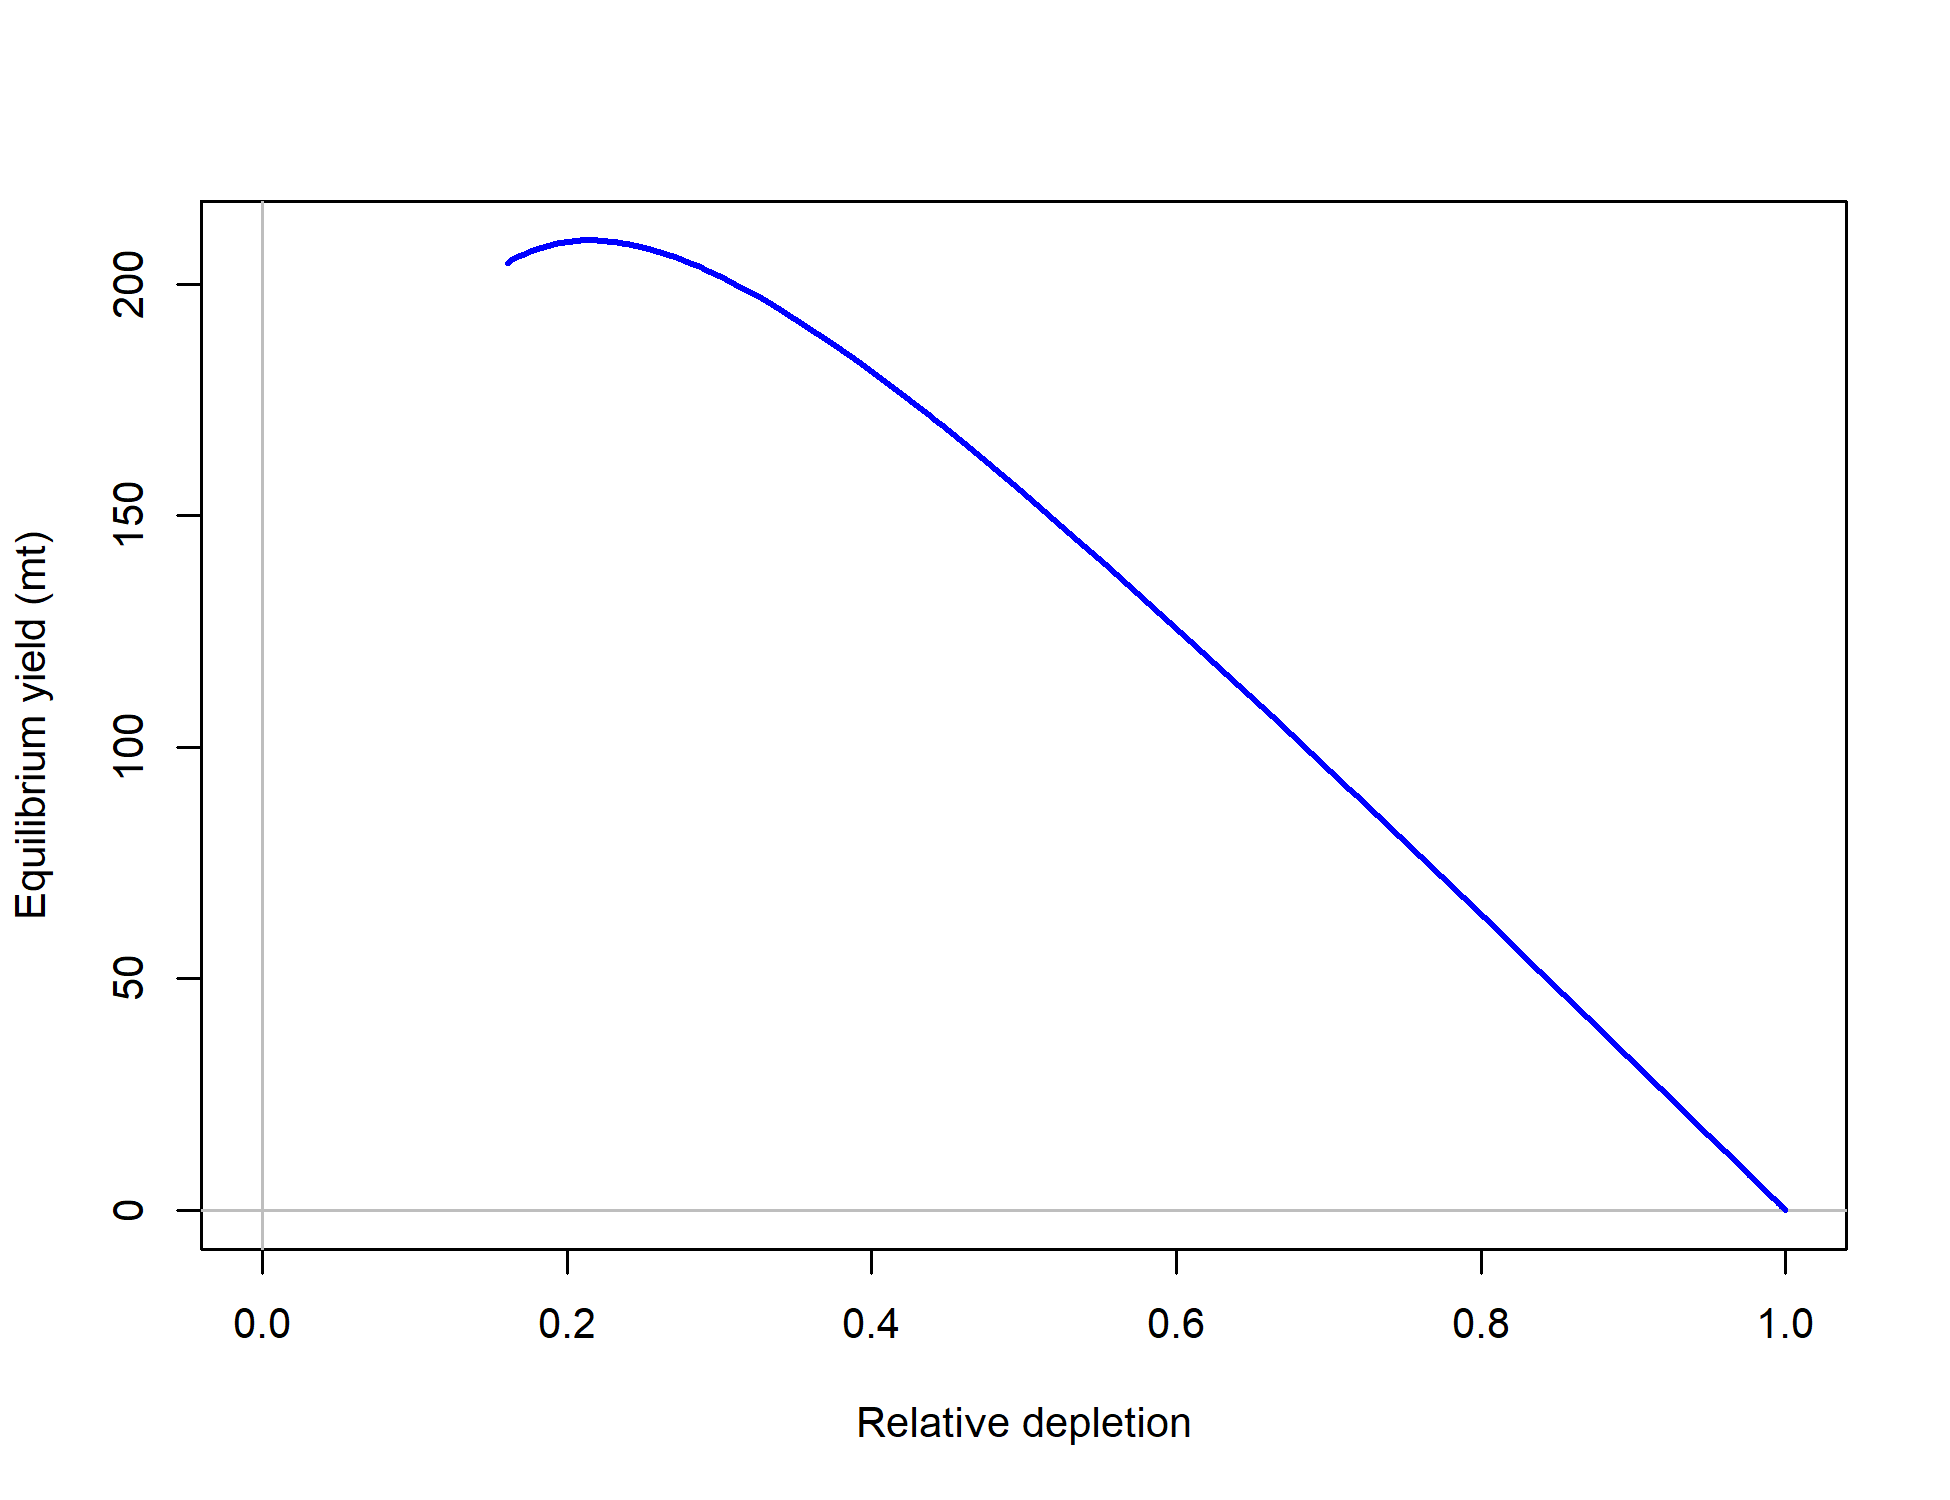
\includegraphics{r4ss/plots_mod1/yield1_yield_curve.png}
\caption{Equilibrium yield curve for the base case model. Values are
based on the 2018 fishery selectivity and with steepness fixed at 0.718.
\label{fig:Yield_all}}
\end{figure}

\FloatBarrier

\newpage

\subsection*{Research and Data Needs}\label{research-and-data-needs}
\addcontentsline{toc}{subsection}{Research and Data Needs}

We recommend the following research be conducted before the next
assessment:

\begin{enumerate}

\item \textbf{xxxx}: 

\item \textbf{xxxx}:

\item \textbf{xxxx}:

\item \textbf{xxxx}:

\item \textbf{xxxx}:

\end{enumerate}

\FloatBarrier

\newpage

\renewcommand{\thefigure}{\arabic{figure}}
\renewcommand{\thetable}{\arabic{table}}

\setcounter{figure}{0} \setcounter{table}{0}

\pagenumbering{arabic}

\section{Introduction}\label{introduction}

\subsection{Basic Information and Life
History}\label{basic-information-and-life-history}

\emph{Population Structure and Complex Assessment Considerations}

There have been a number of analyses conducted on the genetic
differentiation between gopher rockfish and black-and-yellow rockfish.
The studies have yielded some range of results, but have generally
concluded that there is unusually low genetic differentiation between
the two species. The most frequently used measure of genetic analyses to
evaluate evidence for population differentiation is the fixation index
(\(F_{ST}\)), defined as the proportion of the total genetic variation
in one sub-population (subscript S) relative to the total genetic
variation (subscript T) (Hauser and Carvalho
\protect\hyperlink{ref-Hauser2008}{2008}, Waples et al.
\protect\hyperlink{ref-Waples2008}{2008}). Values of \(F_{ST}\) range
from 0 to 1 where a zero value implies the populations are panmictic and
a value closer to one implies the two populations are genetically
independent. Values of \(F_{ST}\) thought to be consistent with
biologically meaningful genetic differentiation and demographic
isolation between populations range from 0.05 to 0.1 (Waples and
Gaggiotti \protect\hyperlink{ref-Waples2006}{2006}). It is also
important to note that \(F_{ST}\) values are dependent on the study's
sample size and it may not necessarily be appropriate to compare them
across studies.

Morphologically, gopher and black-and-yellow rockfishes are almost
indistinct, except for their color variation (Hubbs and Schultz
\protect\hyperlink{ref-Hubbs1933}{1933}). Early efforts to evaluate
whether the two species were genetically distinct began with an allozyme
analysis by Seeb et al. (\protect\hyperlink{ref-Seeb1986}{1986}), which
did not detect genetic differentiation between gopher and
black-and-yellow rockfish. However, as allozymes are proteins that are
often conserved, this early work was not necessarily representative of
genome-wide relationships between the two groups. In a subsequent study
of restriction site polymorphisms, Hunter et al.
(\protect\hyperlink{ref-Hunter1994}{1994}) found slight but significant
differences between species based on restriction fragment length
polymorphisms (RFLP's). Following that study, an analysis of the
mitochondrial control region by Alesandrini and Bernardi
(\protect\hyperlink{ref-Alesandrini1999}{1999}) did not detect
differences between the two species, although mtDNA also has limitations
regarding how results can be extrapolated across the nuclear genome.
Analysis of seven microsatellite loci by Narum et al.
(\protect\hyperlink{ref-Narum2004}{2004}) found an \(F_{ST}\) of 0.049
across the overlapping range of the two species, which provided some
evidence of divergence, although such divergence is relatively low
compared to other species within \emph{Sebastes}. Those authors
characterized their results as suggesting that the two are
``reproductively isolated incipient species.'' Buonaccorsi et al.
(\protect\hyperlink{ref-Buonaccorsi2011}{2011}) found an even lower
\(F_{ST}\) of 0.01 using 25 microsatellite loci, and concluded that
gopher and black-and-yellow rockfish ``have not completed the speciation
process.'' All of these studies are indicative of low levels of genetic
divergence and a high probability of ongoing gene flow between the two
nominal species.

Most recently, an analysis of rockfish species assignment using
microhaplotypes by Baetscher
(\protect\hyperlink{ref-Baetscher2019}{2019}) observed mistaken genetic
assignment of a small number of individuals between gopher and
black-and-yellow rockfishes, while no other species among the 54
rockfishes analyzed resulted in mis-assignments. In addition,
comparisons of \(F_{ST}\) values within the study indicated that the
level of genetic differentiation observed between gopher and
black-and-yellow rockfishes is lower than that observed among all other
pairwise comparisons of the 54 species in the \emph{Sebastes} genus that
were included in their analysis. Baetscher
(\protect\hyperlink{ref-Baetscher2019}{2019}) characterized the results
as suggestive of the two species representing ``sister species with
evidence of ongoing gene flow,'' noting that a more rigorous evaluation
of the level of genetic distinction between these two species would
benefit from whole-genome sequencing of representatives from each
species group.

In addition to the differences in coloration, the depth distribution and
range differ between the two species. The range of both species extends
from Cape Blanco Oregon to Baja California. Both species are uncommon
north of Fort Bragg, California and black-and-yellow rockfish is
uncommon south of Point Conception, California. However, gopher rockfish
can be found as far south as Punta San Roque on the Baja
peninsula.Gopher rockfish are found in rocky reef habitat from the
intertidal to depths of 264 ft (80 m) with a predominant depth
distribution of 30 to 120 ft (9-37 m), while the black-and-yellow
rockfish occupies depths from the intertidal to 120 ft (40 m) and is
predominantly observed in depths shallower than 60 ft (18 m) (Eschmeyer
et al. \protect\hyperlink{ref-Eschmeyer1983}{1983}, Love et al.
\protect\hyperlink{ref-Love2002}{2002}).

Both species are solitary, sedentary, and territorial species with home
ranges of 10-12 square meters (Love et al.
\protect\hyperlink{ref-Love2002}{2002}). A large percentage (67-71\%) of
black-and-yellow rockfish returned to the site of capture within two
weeks after tranlocated within 50 m (Hallacher
\protect\hyperlink{ref-Hallacher1984}{1984}). Lea et al.
(\protect\hyperlink{ref-Lea1999}{1999}) found that gopher rockfish
exhibit minor patterns of movement (\textless{}12.8 km) with all fish
being recaptured on the same reef system where they were tagged.
Matthews (\protect\hyperlink{ref-Matthews1985}{1985}) fround that 11.8\%
of tagged and recaptured gopher rockfish, adn 25\% of black-and-yellwo
rockfish, moved from four low-relief natural reefs to a new high-relief
artificial reef in Monterey Bay. The maximum distance between the
natural and aritifial reefs travelled by gopher or black-and-yellow
rockfish was 1.6 km. After only a year, the fish assemblage on the
artificial reef closely resembled that of the nearby natural reefs. The
paper did no address the spatial segregation of gopher and
black-and-yellow rockfish on the new artificial reef.

Larson (\protect\hyperlink{ref-Larson1980}{1980}) conducted a study on
the territoriality and segregation between gopher and black-and-yellow
rockfishes. When one species was removed, the other extended its depth
range to areas where the other previously occupied, indicating
interspecific competition plays a role in controlling their depth
distributions where both species are present. Of the two species,
black-and-yellow rockfish are socially dominant and aggressive towards
excluding gopher rockfish from shallower waters.

Both species are be feed at night, with similar diets composed primarily
of crabs and shrimp,supplemented by fish and cephalopods (Larson
\protect\hyperlink{ref-Larson1972}{1972},
\protect\hyperlink{ref-Hallacher1985}{1985}, Love et al.
\protect\hyperlink{ref-Love2002}{2002}). Loury et al.
(\protect\hyperlink{ref-Loury2015}{2015}) found no significant
differences in the diet of gopher rockfish inside and outside the 35
year old Point Lobos Marine Protected Area (MPA). She did find the diet
of gopher rockfish at Año Nuevo (shallower and north of Point Lobos) was
dominated by crabs and dominated by brittle stars at southern, deeper
study locations. Zuercher (\protect\hyperlink{ref-Zuercher2019}{2019})
examined the diets of a suite of nearshore rockfish species including
black-and-yellow and found that they relied on hard-bodied benthic
invertebrates such as Brachyuran crabs, shrimps, other arthropods, and
octopus. The diet of black-and-yellow rockfish remained the same across
sampling years, but they occupied a lower trophic level during the
upwelling season.

\subsection{Early Life History}\label{early-life-history}

Gopher and black-and-yellow rockfish have similar juvenile development.
Both rockfish species are viviparous and release one brood per season
between January and July (Echeverria
\protect\hyperlink{ref-Echeverria1987}{1987}). Larvae are approximately
4 mm in length at birth and have a 1-2 month pelagic stage before
recruiting to the kelp forest canopy, i.e., surface fronds of
\emph{Macrosystis pyrifera} and \emph{Cysteoseira osmundacea} at around
15-21 mm (Anderson \protect\hyperlink{ref-Anderson1983}{1983}, Wilson et
al. \protect\hyperlink{ref-Wilson2008}{2008}). The larvae are
transparent until they reach juvenile stage at 22-23 mm. Differences in
coloration between the two sepcies begin to occur at 25-30 mm and can be
used to identify one species from the other. Gopher rockfish become more
orange and brown, while black-and-yellow rockfish become more black and
yellow. Benthic juveniles associate with \emph{Macrosystis} holdfasts
and sporophylls (Anderson \protect\hyperlink{ref-Anderson1983}{1983}).

The juveniles undergo ontogenetic migration down the stalks to deeper
depths, finally settling on rocky reef habitat in their respective adult
depth distribution. Juvenile bocaccio and other fish predate on young of
year and other reef dwelling species including cabezon predate on
post-settlement juveniles. Individuals avoid rough surge conditions and
predators by hiding in the rocky bottom during the daylight hours, then
returning to more open water at dusk (Love et al.
\protect\hyperlink{ref-Love2002}{2002}).

\subsection{Map}\label{map}

A map showing the scope of the assessment and depicting boundaries at
Cape Mendocino to the north and the U.S./ Mexico border at the south
(Figure \ref{fig:assess_region_map1}). The recreational fishing fleet
was split into two fleets at Point Conception.

\subsection{Ecosystem Considerations}\label{ecosystem-considerations-1}

In this assessment, ecosystem considerations were not explicitly
included in the analysis. This is primarily due to a lack of relevant
data and results of analyses (conducted elsewhere) that could contribute
ecosystem-related quantitative information for the assessment.

\subsection{Fishery Information}\label{fishery-information}

The hook-and-line fishery off California developed in the late 19th
century (Love et al. \protect\hyperlink{ref-Love2002}{2002}). The
rockfish trawl fishery was established in the early 1940s, when the
United States became involved in World War II and wartime shortage of
red meat created an increased demand for other sources of protein (Harry
and Morgan \protect\hyperlink{ref-Harry1961}{1961}, Alverson et al.
\protect\hyperlink{ref-Alverson1964}{1964}).

Gopher and black-and-yellow (referred to from hereon as GBRY when
discussing the complex) rockfish have been a minor component of the
commercial and recreational rockfish fishery since at least the late
1960s (CFIS and RecFIN). The commercial catch histories of the two
species cannot easily be separated (Figure
\ref{fig:Catches_livedeadNS_gby}). From 1916-1936 only black-and-yellow
rockfish were reported in the landings, and an average of 0.04 mt of
black-and-yellow rockfish are reported from 1937-1983. Black-and-yellow
rockfish reappear in the landings in 1984 with 7.2 mt landed
commercially. From 1985-1988 the trend switches and only
black-and-yellow rockfish appear in the commercial landings, with gopher
rockfish averaging 0.1 mt landed, and 0 mt reported in 1987. From 1988
and on, the landings are dominated by gopher rockfish, and both species
are represented in the commercial landings.

The landings from south of Point Conception are minor throughout the
time period, with peaks in the 1950s and 60s for gopher rockfish.
Black-and-yellow rockfish are rare south of Point Conception and
expected that these catches are minimal.

The live fish fishery began in the early 1990s, with the first
commercial landings of live gopher rockfish in 1993, and
black-and-yellow rockfish a year later. By 1995 over half (57\%; 39 mt)
of the commercial landings were from the live fish fishery. This
increased quickly over the next few years and has been on average 84\%
of the landed gopher and black-and-yellow rockfish (also referred to
GBYR to reference the complex in this assessment) since 2000. The
majority of the landings are from gopher rockfish north of Point
Conception. Landings of live GBYR south of Point Conception were higher
in the late 1990s, (max. 3.2 mt in 1999), and have been averaging 0.4 mt
since 2003.

The ex-vessel value of GBYR increased from less than \$40,000 in 1984
and peaked at \$680,452 in 1996 (Figure \ref{fig:GBY_revenue}). The
ex-vessel revenue has been fairly stable at around \$500,000 a year
since 2007. Prior to the live fish fishery in 1994, the average price
per pound for either species was around \$2 a pound. The live fish
fishery increased the value of both species to an average of \$6-\$8 a
pound. The maximum reported value of either a gopher or black-and-yellow
rockfish was \$20 a pound in 2003.

The recreational GBYR fishery for California is most prominent north of
Point Conception throughout the entire catch history (Figure
\ref{fig:Exec_catch1}). The recreational landings increased from 1928 to
1980. The sharp increase in the 1980s could be an artifact of the MRFSS
sampling program that began in 1980; however, the more recent
recreational landings also exhibit a cyclical trend of years with high
catches followed by period of decreased recreational landings. The CRFS
era recreational total mortality represents the most accurate
description of the recreational fleet's catches in terms of area, mode
and species (Figure \ref{fig:CFRS_catches}).

Recreational catches are dominated by gopher rockfish north of Point
Conception in the private/rental (PR) and party/charter (PC or CPFV)
modes. South of Point Conception gopher rockfish are predominately
caught by the CPFV fleet, with all other modes being insignificant. The
total recreational mortality of black-and-yellow rockfish south of Point
Conception since 2005 is 3 mt, compared to 106 mt north of Point
Conception. The total mortality since 2005 for gopher rockfish is 86 mt
south of Point Conception and 669 mt north of Point Conception.

\subsection{Summary of Management
History}\label{summary-of-management-history}

Prior to the adoption of the Pacific Coast Groundfish Fishery Management
Plan (FMP) in 1982, GBYR were managed through a regulatory process that
included the California Department of Fish and Wildlife (CDFW) along
with either the California State Legislature or the Fish and Game
Commission (FGC) depending on the sector (recreation or commercial) and
fishery. With implementation of the Pacific Coast Groundfish FMP, GBYR
came under the management authority of the Pacific Fishery Management
Council (PFMC), and were managed as part of the \emph{Sebastes} complex.
Because neither species had undergone rigorous stock assessment and did
not compose a large fraction of the landings they were classified and
managed as part of ``Remaining Rockfish'' under the larger heading of
``Other Rockfish'' (PFMC (\protect\hyperlink{ref-PFMC2002}{2002},
\protect\hyperlink{ref-PFMC2004}{2004})).

Since the early 1980s a number of federal regulatory measures have been
used to manage the commercial rockfish fishery including cumulative trip
limits (generally for two- month periods) and seasons. Starting in 1994
the commercial groundfish fishery sector was divided into two
components: limited entry and open access with specific regulations
designed for each component. Other regulatory actions for the general
rockfish categories have included area closures, gear restrictions, and
cumulative bimonthly trip limits set for the four different commercial
sectors - limited entry fixed gear, limited entry trawl, open access
trawl, and open access non-trawl. Harvest guidelines are also used to
regulate the annual harvest for both the recreational and commercial
sectors.

In 2000, changes in the PFMC's rockfish management structure resulted in
the discontinued use of the \emph{Sebastes} complex, and was replaced
with three species groups: nearshore, shelf, and slope rockfishes
(January 4, 2000; 65 FR 221), of which GBYR are included in the
nearshore group. Within the nearshore group, they are included in the
``shallow nearshore rockfish'' component.

During the late 1990s and early 2000s, major changes also occurred in
the way that California managed its nearshore fishery. The Marine Life
Management Act (MLMA), which was passed in 1998 by the California
Legislature and enacted in 1999, required that the FGC adopt an FMP for
nearshore finfish (Wilson-Vandenberg et al.
\protect\hyperlink{ref-Vandenberg2014}{2014}). It also gave authority to
the FGC to regulate commercial and recreational nearshore fisheries
through FMPs and provided broad authority to adopt regulations for the
nearshore fishery during the time prior to adoption of the nearshore
finfish FMP. Within this legislation, the Legislature also included
commercial size limits for ten nearshore species including GBYR (10-inch
minimum size) and a requirement that commercial fishermen landing these
ten nearshore species possess a nearshore permit.

Following adoption of the Nearshore FMP and accompanying regulations by
the FGC in fall of 2002, the FGC adopted regulations in November 2002
which established a set of marine reserves around the Channel Islands in
southern California (which became effective April 2003). The FGC also
adopted a nearshore restricted access program in December 2002 (which
included the establishment of a Deeper Nearshore Permit) to be effective
starting in the 2003 fishing year.

Also, since the enactment of the MLMA, the Council and State in a
coordinated effort developed and adopted various management
specifications to keep harvest within the harvest targets, including
seasonal and area closures (e.g.~the CCAs; a closure of Cordell Banks to
specific fishing), depth restrictions, minimum size limits, and bag
limits to regulate the recreational fishery and license and permit
regulations, finfish trap permits, gear restrictions, seasonal and area
closures (e.g.~the RCAs and CCAs; a closure of Cordell Banks to specific
fishing), depth restrictions, trip limits, and minimum size limits to
regulate the commercial fishery.

The state of California has adopts regulatory measures to manage the
fishery based on the harvest guidelines set forth by the PFMC. The
commercial open access and limited entry fixed gear sectors have
undergone three different spatial management changes in since 2000.
Since 2005, both have managed the area south of \(40^\circ 10^\prime\)
N. latitude as one area. The open access commercial fishery is managed
based on bimonthly allowable catches, that have ranged from 200 pounds
to 1800 pounds per two months since 2000. From 2005 to 2018, the catch
limits have doubled and are now set at 1200 pounds per two months (for
all months) with March and April remaining closed. The limited entry
fixed year sector has followed the same pattern as the open access
sector with bi-monthly limits and a doubling of the catch since 2005.
The limited entry trawl fleet is managed on monthly limits on an annual
basis. Since 2011, the limit has been 300 pounds per month for non-IFQ
species. A history of California's commercial regulations from 2000-2018
can be found in
\protect\hyperlink{appendix-a.-californias-commercial-fishery-regulations}{Appendix
A}. A 10-inch minimume size limit was implemented in 1999 for the
commercial fleet.

Significant regulatory changed in California's recreational sector began
with a change from unlimited number of hooks and lines allowed in 1999
and prior to no more than three hooks and one line per angler in 2000.
Since 2001, the limit has been no more than two hooks and one line per
angler. There is no size limit in the recreational fishery for gopher or
black-and-yellow rockfish. GBYR are part of the nearshore complex which
has had a sub-bag limit within the rockfish bag limit since 1999. The
nearshore sub-bag limit has been 10 fish since 2005.

California also began spatial management, closures, and depth
restrictions for the recreational fleet in 2000. In general, the
recreational season north of Point Conception extends from April to
December, and south of Point Conception from March to December. In the
area that GBYR are most commonly landed, from Monterey to Morro Bay, the
depth restrictions have been between 30 and 40 fathoms until 2017. In
2017 the depth restrictions were eased by 10 fathoms, opening up fishing
depths along the central California coast that had not been open
consistently since 2002. In both 2017 and 2018, the deepest 10 fathoms
was closed prior to the season in December due to high by-catch rates of
yelloweye rockfish, one of two rockfish species that are still
overfished. A full history of the recreational regulations relating to
the spatial management of the fleet can be found in
\protect\hyperlink{appendix-b.-californias-recreational-fishery-regulations}{Appendix
B}.

\subsection{Management Performance}\label{management-performance-1}

NEED TO FINISH\\
The contribution of GBYR to the minor nearshore rockfish OFLs is
currently derived from two sources: 1) forecasts from Key et al.
(\protect\hyperlink{ref-Key2005}{2005}), from Cape Mendocino to Point
Conception, and 2) a Depletion Corrected Average Catch (DCAC (MacCall
\protect\hyperlink{ref-MacCall2009}{2009})) for the area south of Point
Conception. THe total mortality of the minor nearshore rockfish has been
below the ACL in all years (2011-2016). A summary of these values as
well as other base case summary results can be found in Table
\ref{tab:mnmgt_perform}.

\subsection{Fisheries Off Mexico or
Canada}\label{fisheries-off-mexico-or-canada}

The range of GBYR does not extend north to the Canadian border, and they
are rarely encountered in Oregon and Washington. The southern end of the
gopher rockfish's range extends to Punta San Roque (southern Baja
California) while the southern end of the black-and-yellow rockfish's
range extends to Isla Natividad (central Baja California) (Love et al.
\protect\hyperlink{ref-Love2002}{2002}). However, black-and-yellow
rockfish are rare south of Point Conception, California. This was no
available information on the fishery for GBYR at the time of this
assessment, nor additional details on the abundance or distribution
patterns in Mexican waters.

\section{Assessment}\label{assessment}

\subsection{Data}\label{data}

Data used in the GBYR assessment are summarized in Figure
\ref{fig:data_plot}. Descriptions of the data sources are in the
following sections.

\subsubsection{Commercial Fishery
Landings}\label{commercial-fishery-landings}

\emph{Overview of gopher and black-and-yellow catch history}

Commercial fishery landings for gopher and black-and-yellow rockfishes
have not been reported consistently by species throughout the available
catch history (Figure \ref{fig:Catches_livedeadNS_gby}). The period from
1916-1935 indicates that only black-and-yellow rockfish were landed in
the commercial fishery, which then switched to predominately gopher
rockfish from 1937-1984. From 1985-1988 the landings data suggest that
only black-and-yellow rockfish were landed and not until 1995 are both
species well-represented in the catches. There is no way to tease apart
the historical catches by species and even across north and south of
Point Conception prior to about 1995. This precludes the ability to
model the catch histories for either species accurately. Given these
constraints, all commercial data were combined to represent one
commercial fleet in the assessment. Additional details regarding this
decision are described below.

The stock assessment of gopher rockfish in 2005 did not include
black-and-yellow rockfish landings. A comparison of recreational and
commercial landings from the 2005 assessment to those used in this
assessment suggest the 2005 assessment may have included some
black-and-yellow rockfish landings (Figure
\ref{fig:Assessment_compare}). The 2005 assessment estimated
recreational landings from 1969-1980 based on a ratio of commercial to
recreational landings, where as this assessment makes use of the
California Catch Reconstruction landings estimates (Ralston et al.
\protect\hyperlink{ref-Ralston2010}{2010}).

\emph{Commercial Landings Data Sources}

The California Catch Reconstruction (Ralston et al.
\protect\hyperlink{ref-Ralston2010}{2010}) contains landings estimates
of commercial landings from 1916-1968 and was queried on 4 April 2019
for GBYR. There were no estimated gopher rockfish landings prior to
1937. Landings in this database are divided into trawl and `non-trawl.'
Since the majority of GBYR are caught in the commercial fixed gear
fisheries, only estimated catch in the `non-trawl' was used. A total of
0.154 mt (3.18\%) were removed from Eureka commercial landings (based on
current proportions of commercial catch from north of Cape Mendocino in
Eureka) since the assessment represents the GBYR stock south of Cape
Mendocino. The majority of GBYR commercial landings (avg. 83\%) are
landed in the Monterey and Morro Bay port complexes.

Contemporary landings were extracted from two data sources, the
California Cooperative Groundfish Survey,
\href{https://calcom.psmfc.org/}{CALCOM}) and the Pacific Fisheries
Information Network (\href{https://pacfin.psmfc.org/}{PacFIN}) landings
database. Both databases are based on the same data sources (CALCOM
landing receipts), but apply a catch expansion based on different
algorithms. CALCOM collects information including species composition
data (i.e.~the proportion of species landed in a sampling stratum), and
landing receipts (sometimes called ``fish tickets'') that are a record
of pounds landed in a given stratum. Strata in California are defined by
market category, year, quarter, gear group, port complex, and
disposition (live or dead). Although many market categories are named
after actual species, catch in a given market category can consist of
several species. These data form the basis for the ``expanded''
landings, i.e., species composition data collected by port samplers were
used to allocate pounds recorded on landing receipts to species starting
in 1978. Use of the ``Gopher Rockfish'' or the ``Black-and-Yellow
Rockfish'' categories alone to represent actual landings of GBY would
not be accurate.

See Pearson et al. Appendix C
(\protect\hyperlink{ref-Pearson2008}{2008}) for a simple example of the
expansion calculations for the CALCOM database and a description of the
landings in PacFIN can be found in Sampson and Crone
(\protect\hyperlink{ref-Sampson1997}{1997}). Both databases, including
species compositions, and expanded landings estimates are stored at the
Pacific States Marine Fisheries Commission, a central repository of
commercial landings data for the U.S. West Coast. As a note, CALCOM is
the only source for landings from 1969-1980.

Commercial landings from 1981-2018 were queried for a final time from
the CALCOM database on 4 April 2019 and from PacFIN on 3 June 2019.
There are very small differences in commercial landings between CALCOM
and PacFIN from 1981-2018 (Figure \ref{fig:Calcom_vs_Pacfin}). Landings
estimates from PacFIN were used in the assessment (Table
\ref{tab:CommCatches}). Landings were stratified by year, quarter,
live/dead, market category, gear group, port complex, and source of
species composition data (actual port samples, borrowed samples, or
assumed nominal market category). Data from individual quarters were
aggregated at the year level. Fish landed live or dead were combined,
due to changes over time in the reliability of condition information
(Don Pearson, retired NMFS SWFSC, personal communication). From
1916-1968, on average, 74\% of GBYR were landed north of Point
Conception, which rose to 97\% from 1978-2018. Given the smaller
landings south of Point Conception and the similar length composition of
GBYR north and south of Point Conception, no spatial separation was
considered for the commercial fleet.

\subsubsection{Commercial Discards}\label{commercial-discards}

The West Coast Groundfish Observer Program (WCGOP) provides observer
data on discarding across fishery sectors back to 2003. Gopher and
black-and-yellow rockfishes have species-specific depth-stratified
commercial fishery discard mortality rates (Pacific Fishery Managment
Council \protect\hyperlink{ref-PSMFC2018}{2018}). In consultation with
WCGOP staff, the STAT used estimates of total discard mortality from
WCGOP's Groundfish Expanded Mortality Multiyear (GEMM) report. WCGOP
observes between 1-5\% of nearshore fixed gear landings annually south
of \(40^\circ 10^\prime\) N. latitude (coverage rates available
\href{https://www.nwfsc.noaa.gov/research/divisions/fram/observation/data_products/sector_products.cfm\#ob}{here}).
The expanded estimates of total discard weight by species is calculated
as the ratio of the observed discard weight of the individual species
divided by the observed landed weight from PacFIN landing receipts.
WCGOP discard estimates for the nearshore fixed gear fishery take into
account the depth distribution of landings in order to appropriately
apply the depth-stratified discard mortality rates by species (Somers et
al. \protect\hyperlink{ref-Somers2018}{2018}). The discard mortality for
2018 was estimated as an average of the discard mortality from
2013-2017. Discard mortality was estimated from the period prior to
WCGOP discard estimates (1916-2002) based on the average discard
mortality rate from 2003-2016 (2017 was excluded because 2017 discard
mortality was disproportionately higher than all other years) (Table
\ref{tab:CommCatches}).

\subsubsection{Commercial Fishery Length and Age
Data}\label{commercial-fishery-length-and-age-data}

Biological data from the commercial fisheries that caught GBYR were
extracted from CALCOM on 9 May 2019. The CALCOM length composition data
were catch-weighted to ``expanded'' length the raw length composition
data (Table \ref{tab:length_samples_fishery}). The 2005 assessment used
commercial length composition information from CALCOM, but did not
include black-and-yellow rockfish and is not directly comparable. The
2005 assessment used 2 cm length bins from 16-40 cm, where this
assessment uses 1 cm length bins from 4-40 cm. Sex was not available for
the majority (99.5\%) of the commercial length, and the assessment did
not find sexual dimorphism in growth for either species. We aggregated
the commercial length composition among all gears and regions south of
Cape Mendocino.

Discard length compositions from WCGOP (2003-2017) were expanded based
on the the discard estimates and were aggregated for all regions south
of Cape Mendocino and across all fixed gear fisheries.

A total of 46 ages were available for gopher rockfish from the
commercial fisheries 2009-2011, 2016, and 2018. Though sparse, the data
were included as conditional age-at-length for the commercial fleet.

The input sample sizes for commercial length composition data were
calculated via the Stewart Method for fisheries (Ian Stewart, personal
communication, IPHC):

\begin{center}

Input effN = $N_{\text{trips}} + 0.138 * N_{\text{fish}}$ if $N_{\text{fish}}/N_{\text{trips}}$ is $<$ 44

Input effN = $7.06 * N_{\text{trips}}$ if $N_{\text{fish}}/N_{\text{trips}}$ is $\geq$ 44

\end{center}

Commercial length composition data are made available from PacFIN and
the expanded catch-weight length compositions were provided by Andi
Stephens (NWFSC) processed through the
\href{https://github.com/nwfsc-assess/PacFIN.Utilities}{PacFIN
Utilities} package. We compares differences between the catch-weighted
length composition expansions from CALCOM and PacFIN. We were unable to
reconcile the difference between the two data sets. Sample sizes became
more similar if the PacFIN data were restricted to the same market
categories used by CALCOM in the expansion. However, both data sets
apply other filters that we did not have time to explore. For instance,
in the year 2000, 290 more fish were used in the CALCOM expansion than
in PacFIN, but in 2002, 150 more fish were used in the PacFIN expansions
that were not used in CALCOM. Given these caveats, Figure
\ref{fig:Calcom_vs_pacfin_lengths} shows the percent difference in the
expanded length comps within a year. The biggest difference is in length
bin 32 in 2006. However, the same number of fish and samples were used
to expand the 2006 lengths in both databases, indicating there are also
fundamental differences in how the data are treated. Full documentation
is not available for the PacFIN length composition expansion program.
The base model for this assessment uses the CALCOM length composition
data as described above, but a sensitivity was conducted using the
PacFIN length composition data.

\subsubsection{Recreational Fishery Landings and
Discards}\label{recreational-fishery-landings-and-discards}

\emph{Historical recreational landings and discard, 1928-1980}

Ralston et al. (\protect\hyperlink{ref-Ralston2010}{2010}) reconstructed
estimates of recreational rockfish catch and discard in California,
1928-1980. Reported landings of total rockfish were allocated to species
based on several sources of species composition data. Estimates of GBYR
landings and discard (combined) from 1928-1979 are available from the
SWFSC. For this assessment, historical recreational catch was stratified
by year and area (north and south of Point Conception). The catches of
GBYR reported in Ralston et al.
(\protect\hyperlink{ref-Ralston2010}{2010}) are higher by an order of
magnitude than expected given the more recent catches of GBYR in the
MRFSS and CRFS eras south of Point Conception (Figure
\ref{fig:Catches_original}). The recreational catches estimated by
Ralston et al. (\protect\hyperlink{ref-Ralston2010}{2010}) were
discussed with the paper's co-authors and also Commercial Passenger
Fishing Vessel (CPFV), i.e., party/charter mode, captains in California.
A consensus was reached that the estimated landings did not accurately
represent the historical GBYR landings and an alternative catch stream
should be developed. One possibility for the inflated catches of GBYR in
southern California is that all nearshore shallow species were combined
and all of the nearshore deep species were combined and a constant
relative fraction between the two was used to assign catches to each
combination of CDFW fishing block and year. The fraction of GBYR within
the nearshore shallow species group was likely overestimated.

The California Catch Reconstruction applied a linear ramp from from
1928-1936 that was not altered in this assessment. From 1937-1979 a
linear ramp was developed from the 1936 estimate to the average
recreational landing from 1980 and 1983 (1981-1982 catches interpolated
as described in the next section) of 4.3 mt. The recreational catches
north of Point Conception were not altered from the original catch
reconstruction. The resulting alternate recreational catch streams are
in (Table \ref{tab:Rec_removal} and Figure \ref{fig:Catches_alternate}).

\emph{Marine Recreational Fisheries Statistics Survey (MRFSS),
1980-2003}

From 1980-2003, the Marine Recreational Fisheries Statistics Survey
(MRFSS) executed a dockside (angler intercept) sampling program in
Washington, Oregon, and California (see Holliday et al.
(\protect\hyperlink{ref-Holliday1984}{1984}) for a description of
methods). Data from this survey are available from the Recreational
Fisheries Information Network \href{www.recfin.org}{RecFIN}. RecFIN
serves as a repository for recreational fishery data for California,
Oregon, and Washington. Catch estimates for years 1980-2003 were
downloaded on 23 March 2019, and are consistent from 1992-2004 with the
previous assessment (Key et al. \protect\hyperlink{ref-Key2005}{2005})
(Figure \ref{fig:Assessment_compare}).

MRFSS-era recreational removals for California were estimated for two
regions: north and south of Point Conception. No finer-scale estimates
of landings are available for this period. Catches were downloaded in
numbers and weight. Catch in weight is sometimes missing from the
database due to missing average weight estimates. We estimated average
weights based on adjacent strata as needed, although the effect was
relatively minor (7.4 mt over all years for gopher rockfish and 0.6 mt
for black-and-yellow rockfish). Data were not available for the CPFVs in
Northern California from 1980-1982, and we used the average value from
this mode and region from 1983-1987 for these three years. MRFSS
sampling was temporarily suspended from 1990-1992, and we used linear
interpolation to fill the missing years. Sampling of CPFVs in Northern
California was further delayed, and the linear interpolation spans the
period 1990-1995 for this boat mode and region. Landings data for the
shore-based modes (beach/bank, man-made/jetty and shore) were sparse
throughout the MRFSS sampling. All three shore-based modes were combined
by region and linear interpolations were applied missing data in 1981
for the Northern California and 1995, 1996-2001, and 2004 in Southern
California.

Catches from north of Cape Mendocino were removed based on a CRFS-era
average of fraction of recreational landings north of Cape Mendocino by
mode (3.3\% of shore-based, 0.1\% of CPFV, and 0.2\% of private/rental
were removed). From 1980-1989, San Luis Obispo County was sampled as
part of Southern California (personal observation from MRFSS Type 3
sampler examined catch where county is available for 1980-2004). This
assessment separates the recreational fleet at Point Conception.
Recreational landings were re-allocated from southern California from
1980-1992 by fleet based on the average proportion of recreational
landings in northern California from 1996-2004 (after sampling of the
CPFV fleet in northern California resumed). The average proportion
re-allocated from southern to northern California for the CPFV mode was
85\%, 97\% for the private/rental mode, and 81\% for the shore-based
modes. Data were pooled over all years and modes to estimate the
landings re-allocation for the shore-based modes. Total recreational
landings for 1981 and 1982 were 18.8 mt and 18.6 mt, respectively. These
landings were \textgreater{}60 mt lower than any of the neighboring
years. Landings from 1981-1982 were interpolated from the 1980 and 1983
landings.

\emph{California Recreational Fisheries Survey (CRFS), 2004-2016}

MRFSS was replaced with the California Recreational Fisheries Survey
(CRFS) beginning January 1, 2004. Among other improvements to MRFSS,
CRFS provides higher sampling intensity, finer spatial resolution (6
districts vs.~2 regions), and onboard CPFV sampling. Estimates of catch
from 2004-2018 were downloaded from the RecFIN database a final time on
4 June 2019, We queried and aggregated CRFS data to match the structure
of the MRFSS data, by year, and region (Table \ref{tab:Rec_removal}).
Catches in the shore-based modes are small compared to the CPFV and
private rental modes. All modes are combined, but separated at Point
Conception for two recreational fleets in this assessment, just as was
done for the California Catch Reconstruction and MRFSS time series.

\emph{Recreational Discards}

Recreational discards were only added to the California Catch
Reconstruction landings, as Ralston et al.
(\protect\hyperlink{ref-Ralston2010}{2010}) did not address discards for
the recreational reconstruction. Recreational removals from the
California Department of Fish and Wildlife MRFSS era (1980-2003)
includes catch type A + B1. Catch type A refers to estimates of catch
based on sampler-examined catch. Catch type B1 includes mainly
angler-reported discard, but also angler-reported retained fish that
were unavailable to the sampler during the interview (e.g., fillets).
The CRFS era removals account for depth-stratified discard mortality
rate and the catch time series includes both retained and discarded
catch (total mortality). We calculated the ratio of dead discards to
total mortality from the CRFS era by region and mode. The region average
across modes was applied to the California Catch Reconstruction as a
constant. The result added 4.68\% annually to recreational removals
north of Point Conception and 4.05\% annually to the removals South of
Point Conception). The final time series of landings and discard
mortality are in Table \ref{tab:Rec_removal}.

\subsubsection{Recreational Fishery Length and Age
Data}\label{recreational-fishery-length-and-age-data}

Recreational length composition samples for California were obtained
from several sources, depending on the time period and boat mode (Table
\ref{tab:length_samples_fishery}). This assessment makes use of a much
longer time series of length composition data, relative to the previous
assessment, as described below. Input sample sizes for recreational
length composition data were based on the number of observed trips, when
available. Other proxies that were used to estimate the number of trips
are described below.

There were no standardized coastwide surveys measure retained or
discarded fish from the recreational fleet prior to 1980.

\emph{CPFV length composition data, 1959-1978}

The earliest available length data for this assessment were described by
Karpov et al. (\protect\hyperlink{ref-Karpov1995}{1995}), who assembled
a time series (1959-1972) of available California CPFV length data (made
available courtesy of W. Van Buskirk). For GBYR, data from 1959-1961 and
1966 were available north of Point Conception and from 1959-1961 from
south of Pt Conception. A total of 716 (680 north of Point Conception)
unsexed measurements of retained fish (no discards) were included in the
assessment (Table \ref{tab:length_samples_fishery}). Sampling of these
length data did not follow a consistent protocol over time and areas
(data are unweighted), and therefore may not be representative of total
catch. Since the number of trips sampled was not reported by Karpov et
al. (1995), we assume the number of sampled trips is proportional to the
number of measured fish in each year, and estimated the number of trips
using the ratio of fish measured per trip in the MRFSS data (roughly 10
fish per trip).

Collins and Crooke (n.d.) conducted an onboard observer survey of the
CPFV fleet in southern California from 1975-1978. A total of 1,308 GBYR
lengths were available from the study and were assumed to all be from
retained fish. Ally et al. (\protect\hyperlink{ref-Ally1991}{1991})
conducted an onboard observer program of the CPFV fleet from 1985-1987
in southern California. Because MRFSS data were available for this time
period as well and represents multiple recreational modes, the Ally et
al. (\protect\hyperlink{ref-Ally1991}{1991}) length data were not used
in the assessment.

\emph{MRFSS Recreational Length Data, 1980-1989 and 1993-2003}

Unsexed length data of retained fish were collected by MRFSS dockside
samplers and downloaded from the RecFIN website. We identified a subset
of lengths that were converted from weight measurements, and these were
excluded from the final data set (Table
\ref{tab:length_samples_fishery}). The length measurements from Collins
and Crooke (n.d.) from 1975-1978 are assumed to all be from retained
fish. As of 2003, the CDFW Onboard Observer program has taken length
measurements for discarded fish. The retained catch is measured during
the dockside (angler intercept) surveys.

The number of CPFV trips used as initial sample sizes for the MRFSS was
based on the number of CPFV trips was determined from the trip-level
MRFS CPFV database and the number of private boat trips was determined
based on unique combinations of the variables ASSNID ,ID\_CODE,
MODE\_FX, AREA\_X, DIST, INTSITE, HRSF, CNTRBTRS, SUB\_REG, WAVE, YEAR,
and CNTY in the Type 3 (sampler-examined catch) data.

During the recent restructuring of the CRFS data on RecFIN, a ``trip''
identifier was not carried over for all modes, and trip-level sample
sizes could not be extracted from the biological detail table on RecFIN.
A proxy for initial sample sizes for 2004-2018 were developed using the
2015 data for which I had access to raw data files by mode from CDFW. In
more recent years, sampling of the shore-based modes has declined and
were not sampled at all in 2018. Samples sizes were calculated by mode
as the number of port-days (or site-days for shore-based modes) during
bi-weekly intervals (e.g., Jan 1-15, Jan 16-31, etc). The number of
port-days sampled in the bi-weekly intervals was used as the initial
sample size for number of trips to calculate initial input sample sizes
using Ian Stewart's method (described above). All length data were
re-weighted in the assessment model.

\subsubsection{Fishery-Dependent Indices of
Abundance}\label{fishery-dependent-indices-of-abundance}

A summary of all indices in the assessment can be found in Table
\ref{tab:Index_summary}. Figure \ref{fig:All_index_compare} shows each
index scaled to the mean value of that index to show them all on the
same scale, i.e., the mean of each index in teh plot is 1.

\textbf{MRFSS Dockside CPFV Index}

From 1980 to 2003 the MRFSS program conducted dockside intercept surveys
of recreational fishing fleet. The program was temporarily suspended
from 1990-1992 due to lack of funding. For purposes of this assessment,
the MRFSS time series was truncated at 1998 due to sampling overlap with
the onboard observer program (i.e., the same observer samples the catch
while onboard the vessel and also conducts the dockside intercept survey
for the same vessel). Each entry in the RecFIN Type 3 database
corresponds to a single fish examined by a sampler at a particular
survey site. Since only a subset of the catch may be sampled, each
record also identifies the total number of that species possessed by the
group of anglers being interviewed. The number of anglers and the hours
fished are also recorded. The data, as they exist in RecFIN, do not
indicate which records belong to the same boat trip. A description of
the algorithms and process used to aggregate the RecFIN records to the
trip level is outlined Supplemental Materials (``Identifying Trips in
RecFIN'').

Initial trip filters included eliminating trips targeting species caught
near the surface waters for all or part of the trip, including trips
with catch of bluefin tuna, yellowfin tuna, skipjack, and albacore.

The following filtering steps were applied to gopher rockfish, as well
as the sum of the two species to represent GBYR. No filtering or indices
were developed for black-and-yellow rockfish alone due to the sparseness
in the data. In the raw data, unfiltered data, black-and-yellow rockfish
only occurred in 48 trips that did not also observer gopher rockfish.
There were an additional 65 trips that encountered both species. There
was little difference between indices developed for gopher-only and the
GBYR complex for both north and south of Point Conception (Figure
\ref{fig:MRFSS_index_compare}). The descriptions of the filtering and
data below represent those for the GBYR complex.

The species composition of catch in California varies greatly with
latitude.\\
Therefore, Stephens-MacCall filtering was applied independently for
north and south of Point Conception. Separate indices were also
developed to represent two recreational fleets in the model.

Since recreational fishing trips target a wide variety of species,
standardization of the catch rates requires selecting trips that are
likely to have fished in habitats containing GBYR. The Stephens-MacCall
(\protect\hyperlink{ref-Stephens2004}{2004}) filtering approach was used
to identify trips with a high probability of catching GBYR, based on the
species composition of the catch in a given trip. Prior to applying the
Stephens-MacCall filter, we identified potentially informative predictor
species, i.e., species with sufficient sample sizes and temporal
coverage (at least 30 positive trips total) to inform the binomial
model. Coefficients from the Stephens-MacCall analysis (a binomial GLM)
are positive for species which co-occur with GBYR, and negative for
species that are not caught with GBYR. Each of these filtering steps and
the resulting number of trips remaining in the sampling frame are
provided in Table \ref{tab:Fleet10_11_Filter}.

\emph{MRFSS Filtering and Index Standardization for North of Point
Conception.} Prior to the Stephens-MacCall filter, a total of 2,788
trips were retained for the analysis. As expected, positive indicators
of GBYR trips include several species of nearshore rockfish, treefish,
kelp rockfish, and blue rockfish, and the strongest counter-indicator
was striped bass (Figure \ref{fig:Fleet10_SM_filter}). While the filter
is useful in identifying co-occurring or non-occurring species assuming
all effort was exerted in pursuit of a single target, the targeting of
more than one target species can result in co-occurrence of species in
the catch that do not truly co-occur in terms of habitat associations
informative for an index of abundance. Stpehens and MacCall (Stephens
and MacCall \protect\hyperlink{ref-Stephens2004}{2004}) recommended
including all trips above a threshold where the false negatives and
false positives are equally balanced. However, this does not have any
biological relevance and for this data set, we assume that if a GBYR was
landed, the anglers had to have fished in appropriate habitat,
especially given how territorial GBYR and both species are strongly
associated with rocky habitat.

Two levels of possible filtering were applied using the Stephens-MacCall
filter (Table \ref{tab:Fleet10_11_Filter}). The Stephens-MacCall
filtering method identified the probability of occurrence (in this case
0.4) at which the rate of ``false positives'' equals ``false
negatives.'' The trips selected using this criteria were compared to an
alternative method including all the ``false positive'' trips,
regardless of the probability of encountering GBYR (Table
\ref{tab:Fleet10_contingency}). This assumes that if GBYR were caught,
the anglers must have fished in appropriate habitat during the trip. The
catch included in this index is ``sampler-examined'' and the samplers
are well trained in species identification. The last filter applied was
to exclude years after 1999 due to a number of regulation changes, and
years in which there were less than 20 observed trips. The final index
is represented by 544 trips, 220 of which encountered GBYR.

Due to the large number of zeros in the data, we modeled catch per
angler hour (CPUE; number of fish per angler hour) using maximum
likelihood and Bayesian negative binomial regression. Models
incorporating temporal (year, 2-month waves) and geographic (region and
area\_x) factors were evaluated. Counties were grouped into three
regions, north of Sonoma county, Sonoma county through Santa Cruz
county, and San Luis Obispo county. Based on AIC values from maximum
likelihood fits (Table \ref{tab:Fleet10_AIC}), a main effects model
including all factors (year, region, area\_x, and 2-month waves) was fit
in the ``rstanarm'' R package (version 2.18.2). Diagnostic checks of the
Bayesian model fit (Neff, Rhat, and Monte Carlo standard error values)
were all reasonable. Predicted means by stratum (Year) were strongly
correlated with observed means, suggesting a reasonable fit to the data
(Figure \ref{fig:Fleet10_MLE_stan}). The NB model generated data sets
with roughly 50-70\% zeros, compared to the observed 60\% (Figure
\ref{fig:Fleet10_prop_zero_STAN}).

The index represents the years 1984-1989, 1995, 1996 and 1999. There is
not a lot of contrast in the index, except for a small increase in 1986.
The final index values and associated log standard error included in the
assessment can be found in Table \ref{tab:Indices}.

\emph{MRFSS Filtering and Index Standardization for South of Point
Conception.} Prior to the Stephens-MacCall filter, a total of 7,334
trips were available for the analysis. As expected, positive indicators
of GBYR trips included several nearshore species, e.g., kelp rockfish,
treefish, and black croaker, while the strongest counter-indicator was
opaleye (Figure \ref{fig:Fleet11_SM_filter}). While the filter is useful
in identifying co-occurring or non-occurring species assuming all effort
was exerted in pursuit of a single target, the targeting of more than
one target species can result in co-occurrence of species in the catch
that do not truly co-occur in terms of habitat associations informative
for an index of abundance.

For consistency with the methods used north of Point Conception (Table
\ref{tab:Fleet10_11_Filter}) the index includes the trips identified as
``false positives'' from the Stephens-MacCall filtering that had a lower
threshold level of 0.22 (Table \ref{tab:Fleet11_contingency}). The last
filter applied was to exclude years after 1999 due to a number of
regulation changes, and years in which there were less than 20 observed
trips. The final index is represented by 475 trips, 342 of which
encountered GBYR.

Catch per angler hour (CPUE; number of fish per angler hour) was
modelled using the delta-GLM approach (Lo et al.
\protect\hyperlink{ref-Lo1992}{1992}, Stefánsson
\protect\hyperlink{ref-Stefansson1996}{1996}). A negative binomial model
was explored, but the proportion of zeroes was not well estimated in the
negative binomial models. This is likely due to the facts that MRFSS
sampling effort was higher south of Point Conception, and GBYR are also
rare south of Point Conception, both leading to a higher proportion of
zeroes in the trip data than for north of Point Conception.

Model selection using Akaike Information Criterion (AIC) supported
inclusion of year, region, area\_x, and 2-month waves. Counties were
grouped into three regions, Santa Barbara to Ventura counties, Los
Angeles and Orange counties, and San Diego county for both the positive
observation model and the binomial model. Area\_x is a measure of
distance from shore, a categorical variable indicating whether most of
the fishing occurred inside or outside three nautical miles from shore.

The resulting index for south of Point Conception represents different
years than the index for north of Point Conception (Table
\ref{tab:Indices}). The index starts in 1980 with continuous data
through 1986, and three additional years in 1996, 1998 and 1999. The
index increases through 1983 and a marked decrease to 1986. The index
for the three years in the 1990s does not exhibit any significant trend.

\textbf{CPFV Onboard Observer Surveys}

Onboard observer survey data were available from three sources for this
assessment, 1) a CDFW survey in central California from 1987-1998
(referred to as the Deb Wilson-Vandenberg onboard observer survey,
(Reilly et al. \protect\hyperlink{ref-Reilly1998}{1998})), 2) the CDFW
CPFV onboard observer survey from 1999-2018, and 3) a Cal Poly survey
from 2003-2018. During an onboard observer trip the sampler rides along
on the CPFV and records location-specific catch and discard information
to the species level for a subset of anglers onboard the vessel. The
subset of observed anglers is usually a maximum of 15 people the
observed anglers change during each fishing stop. The catch cannot be
linked to an individual, but rather to a specific fishing location. The
sampler also records the starting and ending time, number of anglers
observed, starting and ending depth, and measures discarded fish.\\
The fine-scale catch and effort data allow us to better filter the data
for indices to fishing stops within suitable habitat for the target
species.

California implemented a statewide sampling program in 1999 (Monk et al.
\protect\hyperlink{ref-Monk2014}{2014}). California Polytechnic State
University (Cal Poly) has conducted an independent onboard sampling
program as of 2003 for boats in Port San Luis and Morro Bay, and follows
the protocols established in Reilly et al.
(\protect\hyperlink{ref-Reilly1998}{1998}). Cal Poly has modified
protocols reflect sampling changes that CDFW has also adopted, e.g.,
observing fish as they are encountered instead of at the level of a
fisher's bag. Therefore, the Cal Poly data area incorporated in the same
index as the CDFW data from 1999-2018. The only difference is that Cal
Poly measures the lenght of both retained and discarded fish.

We generated separate relative indices of abundance in for the 1987-1999
and 2000-2018 data sets due to the number of regulation changes
occurring throughout the time period (see
\protect\hyperlink{appendix-b.-californias-recreational-fishery-regulations}{Appendix
B}). Separate indices were also developed for north and south of Point
Conception.

\emph{Deb Wilson-Vandenberg Onboard Observer Index Filtering and
Standardization.} The specific fishing locations at each fishing stop
were recorded at a finer scale than the catch data for this survey. We
aggregated the relevant location information (time and number of
observed anglers) to match the available catch information. Between
April 1987 and July 1992 the number of observed anglers was not recorded
for each fishing stop, but the number of anglers aboard the vessel is
available. We imputed the number of observed anglers using the number of
anglers aboard the vessel and the number of observed anglers at each
fishing stop from the August 1992-December 1998 data (see Supplemental
materials for details). In 1987, trips were only observed in Monterey,
CA and were therefore excluded from the analysis. The years 1990 and
1991 were also removed for low sample sizes. Final data filters included
removing reefs that never encountered GBYR, drifts that had fishing
times outside 95\% of the data, and fishing stops with depths
\textless{}9 m and \textgreater{}69m. The final data set contained 2,411
fishing stops, with 1,096 of those encountering GBYR (Figure
\ref{fig:DebWV_sites}).

The index was fit using a delta-GLM model, with a lognormal model (AIC:
1,088) selected over a gamma model (AIC: 1,143) for the positive
encounters. Covariates considered in the full model included year,
depth, and month (Table \ref{tab:Fleet5_AIC}). The model selected by AIC
for both the lognormal and binomial components of the delta-GLM included
year, depth and reef. Depth was included in 10 m depth bins and eight
reefs were select in the final model (Figure coming). The final index
did not indicate an increasing trend that was seen in the 2005 gopher
rockfish assessment using the same data set (Figure
\ref{fig:DebWV_index_compare}). A number of reasons include that
finer-scale location data was keypunched in 2012 for this survey, the
index in this assessment includes black-and-yellow rockfish, and
different filters were applied to the data. However, the the same peaks
and decreases in the two indices are present.

\emph{CDFW and Cal Poly Onboard Observer Index Filtering and
Standardization} As described above the CDFW and Cal Poly onboard
observer programs are identical in that the same protocols are followed.
The only difference is that Cal Poly measures both retained and
discarded fish from the observed anglers. CDFW measures discarded fish
only from the observed anglers, and measures retained fish as part of
the angler interview at the bag level. Cal Poly has also begun
collecting otoliths during the onboard observer trips, which are used as
conditional age-at-length data the recreational fishery north of Point
Conception in this assessment.

A number of filters are applied to these data. All of the Cal Poly data
have been through a QA/QC process once key-punched, whereas a number of
errors remain in the data from CDFW. Data sheets from CDFW are not
longer available prior to 2012 and staff constraints have also prevented
a quality control review of the data.

Each drift was assigned to a reef (hard bottom). Hard bottom was
extracted from the
\href{http://seafloor.otterlabs.org/index.html}{California Seafloor
Mapping Project}, with bathymetric data from state waters available at a
2 m resolution. Reefs were developed based on a number of factors
described in the supplemental material (``Reef Delination'').

Initial filters were applied to the entire data set, north and south of
Point Conception combined. After an initial clean-up of the data, 67,850
drifts remained, with GBYR present in 9,317 (Table
\ref{tab:Fleet6_7_Filter}). This was reduced to 25,427 drifts GBYR
present in 7,250 drifts) after filtering the data to remove potential
outliers in the time fished and observed anglers, limiting the data to
reefs that observed GBYR and were sampled in at least 2/3 of all years,
and to drifts with starting locations within 1,000 m of a reef.

Recreational fishing trips north and south of Point Conception can be
fundamentally different due to differences in habitat structure, target
species, and weather.

\emph{Filtering and Index Standardization for north of Point Conception}
The number of drifts remaining before region specific filtering was
13,792, with 6,036 drifts encountering GBYR (Table
\ref{tab:Fleet6_7_Filter}).\\
Because GBYR are strongly associated with hard bottom habitat, the
distance from a reef at the start of a drift was re-examined for drifts
encountering GBYR. The maximum distance was 872 m, but the 97\% quantile
dropped to 42 m and was chosen as a reasonable cutoff value, and only
resulted in a reduction of 182 drifts that encountered gopher rockfish.
The final data were filtered to ensure all selected reefs were sampled
in at least 2/3 of all years, leaving 12,965 drifts for the final index,
5,796 of which encountered GBYR (Figure
\ref{fig:Onboard_observer_north_sites}).

The index of abundance was modeled with the a delta-GLM modeling
approach, with year, month, 10 m depth bins from 10-59 m, and 12 reefs
as possible covariates. A lognormal model (AIC: 12,185) was selected
over a gamma (AIC: 12,520) for the positive observations using AIC. The
full model was selected by AIC for the lognormal and binomial components
of the delta-GLM. The index indicates a relatively stable trend from
2001-2009 and a steady decrease from 2010-2013. The relative index of
abundance has increased since 2014.

\emph{Filtering and Index Standardization for south of Point Conception}
The bathymetric data is not available at as fine-scale resolution for
the Southern California Bight and more of the trips and drifts target
mid-water species, including mid-water rockfish (Table
\ref{tab:Fleet6_7_Filter}). Therefore, instead of using distance to reef
as a filter, we filtered the data to drifts that encountered 20\% or
more groundfish. This resulted in the total number of drifts decreasing
from 11,635 to 5,495, but only decreased the number of drifts
encountering GBYR from 1,277 to 1,171. A final check was made to ensure
all reefs were sampled in at least 2/3 of all years, leaving 5,440 drift
for the final index, of which 1,132 encountered GBYR (Figure
\ref{fig:Onboard_observer_south_sites}).

The index of abundance was modeled with the a delta-GLM modeling
approach, with year, month, 10 m depth bins from 10-59 m, and four reefs
as possible covariates. A lognormal model (AIC: 162) was selected over a
gamma (AIC: 277) for the positive observations using AIC. A model with
year, depth and reef was selected by AIC for both the lognormal and
binomial components of the delta-GLM. The index indicates a relatively
stable trend from 2001-2004 and a steady increase from 2005-2017.

\subsubsection{Fishery-Depenent Indices: Availabe Length and Age
Data}\label{fishery-depenent-indices-availabe-length-and-age-data}

Length data associated with the MRFSS dockside CPFV survey and the
current onboard observer surveys conducted by CDFW are incorporated into
the biological data pulled from the respective data sources, MRFSS and
CRFS. The additional length data are not incorporated as separate length
composition data as they represent the same portion of the population
sampled by the CDFW onboard observer program.

Cal Poly collected ototlihs from the onboard observer program starting
in 2017 as part of a special study to correlate fish length before and
and after the fish was filleted by the deckhands onboard the CPFV
vessels. All fish collected in 2017 only had associated post-fillet
lengths and were not used in the assessment since the study has not been
finalized nor has the method been endorsed by the SSC. A subset of fish
form the 2018 collection included both pre- and post-fillet length and
were used in the assessment as conditional age-at-length data associated
with the recreational fleet north of Point Conception.

Length composition from Deb Wilson-Vandenberg's onboard observer survey
are included in the asessment. This program measured both retained and
discarded fish, and represent the portion of the population sampled with
the spatial extent of the index. This onboard observer program continued
during the period from 1990-1992 when MRFSS was on hiatus.

\subsubsection{Fishery-Independent Data
Sources}\label{fishery-independent-data-sources}

Neither of the two fishery-independent surveys described below have
previously been used in stock assessments as indices of abundance.

\textbf{California Collaborative Fisheries Research Project}

The California Collaborative Fisheries Research Project,
\href{https://www.mlml.calstate.edu/ccfrp/}{CCFRP}, is a
fishery-independent hook-and-line survey designed to monitor nearshore
fish populations at a series of sampling locations both inside and
adjacent to MPAs along the central California coast (Wendt and Starr
\protect\hyperlink{ref-Wendt2009}{2009}, Starr et al.
\protect\hyperlink{ref-Starr2015}{2015}). The CCFRP survey began in 2007
and was originally designed as a statewide program in collaboration with
NMFS scientists and fishermen. From 2007-2016 the CCFRP project was
focused on the central California coast, and has monitored four MPAs
consistently since then (Figure \ref{fig:CCFRP_sites}). In 2017, the
program was expanded coastwide within California. The index of abundance
was developed from the four MPAs sampled consistently (Año Nuevo and
Point Lobos by Moss Landing Marine Labs; Point Buchon and Piedras
Blancas by Cal Poly).

The survey design for CCFRP consists a number 500 x 500 m cells both
within and outside each MPA. On any given survey day for a chose site
cells are randomly selected within a stratum (MPA and/or reference
cells). CPFVs are chartered for the survey and the fishing captain is
allowed to search within the cell for a fishing location. During a
sampling event, each cell is fished for a total of 45? minutes by
volunteer anglers. Each fish encountered is recorded, measured, and can
be linked back to a particular angler, and released (or descended to
depth). Starting in 2017, a subset of fish have been retained to collect
otoliths and fin clips, needed biological information for nearshore
species. For the index of abundance, CPUE was modelled at the level of
the drift, similar to the fishery-dependent onboard observer survey
described above.

The CCFRP data are quality controlled at the time they are key punched
and little filtering was needed for the index. Cells not consistently
sampled over time were excluded as well as cells that never encountered
GBYR. CCFRP samples shallower depths to avoid barotrauma-induced
mortality. The index was constrained to 5-39m in 5 m depth bins. The
final index included 4,920 drifts, 3,848 of which encountered GBYR.

We modeled catch per angler hour (CPUE; number of fish per angler hour)
using maximum likelihood and Bayesian negative binomial regression. The
proportion of zeroes in this data was relatively small (22\%), and if
overdispersion were not present, the regression would innately become
Poisson. Models incorporating temporal (year, month) and geographic (MPA
site and MPA vs Reference cells) factors were evaluated. Based on AIC
values from maximum likelihood fits (Table \ref{tab:Fleet9_AIC}), a main
effects model including all factors (year, month, site and MPA/REF) was
fit in the ``rstanarm'' R package (version 2.18.2). Diagnostic checks of
the Bayesian model fit (Neff, Rhat, and Monte Carlo standard error
values) were all reasonable. Predicted means by stratum (Year) were
strongly correlated with observed means, suggesting a reasonable fit to
the data (Figure \ref{fig:Fleet9_MLE_stan}). The NB model generated data
sets with roughly 18-22\% zeros, compared to the observed 22\% (Figure
\ref{fig:Fleet10_prop_zero_STAN}).

The CCFRP index of abundance closely matches the trend observers in the
onboard observer index from 2009-2018 (Figure
\ref{fig:All_index_compare}). The index decreases from 2009 to 2013, and
then exhibits the same increase through 2018. When both indices are
standardized to their means, the values for 2013 and 2018 are the same.

\emph{CCFRP Length Measurements and Available Ages}

The CCFRP program measures every fish encountered to the nearsest half
centimeter. A total of 22,470 GBYR were measured by CCFRP from
2007-2018, of which only 212 were black-and-yellow rockfish. The length
distributions for each of the four MPAs used in the index for this
assessment show slight difference in their peaks (Figure
\ref{CCFRP_lengths_by_site}). Año Nuevo is the most northern site and
Point Buchon the most southern.

Conditional age-at-lenght data were also incorporated into the
assessment from the CCFRP program, including two master's theses that
are products of the CCFRP. Erin Loury (Loury
\protect\hyperlink{ref-Loury2011}{2011}) collected gopher rockfish
otoliths as part of her thesis work from 2007-2009 that included
specimens from both inside and outside the MPAs. Natasha Meyers-Cherry
(Meyers-Cherry \protect\hyperlink{ref-MeyersCherry2014}{2014}) conducted
another thesis focused on the life history of gopher rockfish and
collected otoliths from 2011-2012, also both inside and outside the
MPAs. Both MLML and Cal Poly began routinely collecting otoliths from a
select number of fish in 2017 as part of the CCFRP program. Also
included in the conditional age-at-length dat for this fleet are
ototliths collected in 2018 by the University of California Davis Bodega
Marine Lab CCFRP program.

\textbf{Partnership for Interdisciplinary Studies of Coastal Oceans}

The Partnership for Interdisciplinary Studies of Coastal Oceans,
\href{http://www.piscoweb.org/kelp-forest-study}{PISCO-UCSC}, conducts a
number of surveys to monitor the kelp forests, one of which is a kelp
forest fish survey. PISCO has monitored fish population in the 0-20 m
depth range as part of the Marine Life Protection Act (MLPA) since 1998.
Paired sites inside and outside MPAs are surveyed to monitor the
long-term dynamics of the kelp forest ecosystem and provide insight into
the effect of MPAs on kelp forest species. PISCO conducts the fish
surveys from late July through September. At each site, benthic,
midwater, and canopy scuba transcets are conducted at 5, 10, 15, and 20
m depth. All divers are trained in species identification. Along each 30
m transect, divers enumerate all identifiable non-cryptic fish, and
measure total length to the nearest centimeter. PISCO surveys are
conducted by the University of California Santa Cruz (UCSC) in central
California and through the University of California Santa Barbara in
southern California. All PISCO data were provided by Dan Malone (UCSC).

The majority of filtering for the PISCO data set was to determine which
sites to keep for the final index. After initial filtering the data for
GBYR in southern California were too sparse to be considered for the
index of abundance. Gopher and black-and-yellow rockfish were also
rarely observed in the midwater and canopy transects, and therefore the
index is based only on the benthic transects. Only sites sampled
consistently throughout the time period 2001-2018 were kept for the
index. Multiple transects can be conducted along the same line within a
sampling event. All transects within a site were combined and effort was
modeled as the number of transects represented in the number of fish
observed. The final index included 3,231 transects, of which 1,729
observed GBYR (Figure \ref{fig:PISCO_sites}).

We modeled number of fish observed per transect(s) using maximum
likelihood and Bayesian negative binomial regression. Models
incorporating temporal (year, month) and geographic (site and zone)
factors were evaluated. The zone is a factor indicating the depth
stratification at a site, i.e., 5 m,10 m,15 m, or 20 m targetted bottom
depth.. Based on AIC values from maximum likelihood fits (Table
\ref{tab:Fleet8_AIC}), a main effects model including all factors (year,
month, site and zone) was fit in the ``rstanarm'' R package (version
2.18.2). Diagnostic checks of the Bayesian model fit (Neff, Rhat, and
Monte Carlo standard error values) were all reasonable. Predicted means
by stratum (Year) were strongly correlated with observed means,
suggesting a reasonable fit to the data (Figure
\ref{fig:Fleet8_MLE_stan}). The NB model generated data sets with
roughly 16-25\% zeros, compared to the observed 23\% (Figure
\ref{fig:Fleet8_prop_zero_STAN}).

The final index decreases from 2001 to the late 2000s, with lower
estiamtes of relative abundance from 2005-2010. From 2010 to 2015, the
index increaes and peaks in 2015, before the decreasing trends from
2016-2018. The pattern observed in this index indicates almost an
counter trend to that observed in the onboard observer and CCFRP indices
for north of Point Conception (Figure \ref{fig:All_index_compare}). The
PISCO survey is sampling different habitat types than the other two
surveys, and covers much shallower depths.

\emph{PISCO Length Measurements}

Every GBYR observed by PISCO divers except one, had an associated length
measurement (N = 11,965). Divers measure fish to the nearest centimeter,
and are trained to measure fish underwater and be aware of possible
biases, e.g., ambient light, body color, visibility, and body shape.
Both juvenile and adult GBYR were observed in the PISCO kelp forest fish
survey data (Figure \ref{fig:PISCO_lengths}). Of note is the similarity
in length distibutions both between the species and for the two species
combined across sites. Fish in the 10-17 cm size range (approximately)
are not observed in this survey. There is significant post-settlement
mortality for both species, which is thought to be due to
density-dependent predation (Johnson
\protect\hyperlink{ref-Johnson2006}{2006},
\protect\hyperlink{ref-Johnson2007}{2007}). Secondly, both species are
cryptic and observed more often at night than during the day (Mark Carr,
PISCO-UCSC, personal communication).

\subsubsection{Biological Parameters and
Data}\label{biological-parameters-and-data}

Neither gophr nor black-and-yellow rockfish have forked tails, therefore
total legnth and fork length are equal. All of the data provided for
this assessment were either in fork length or total length.

(Table \ref{tab:length_samples_survey})

\textbf{Length and Age Compositions}

Length compositions were provided from the following sources:

\begin{itemize}[noitemsep,nolistsep,topsep=0pt]
  \item CALCOM (\emph{commercial retained dead fish}, 1987, 1992-2018)   
  \item WCGOP (\emph{commercial discarded fish}, 2004-2018)    
  \item Deb Wilson-Vandenber's onboard observer survey (\emph{recreational charter retained and discarded catch}, 1987-1998)
  \item California recreational sources combined (\emph{recreational charter retained catch})     
    \begin{itemize}[noitemsep,nolistsep]
      \item Miller and Gotshall dockside survey (1959-1966)    
      \item Ally  et al. onboard observer survey (1985-1987)
      \item Collins and Crooke onboard observer survey (1975-1978)     
      \item MRFSS dockside survey (1980-2003)     
      \item CRFS onboard and dockside survey (2004-2018)
    \end{itemize}
 \item PISCO dive survey (\emph{research}, 2001-2018)      
 \item CCFRP hook-and-line survey (\emph{research}, 2007-2018)        
\end{itemize}

The length composition of all fisheries aggregated across time by fleet
is in Figure \ref{fig:comp_lendat_aggregated_across_time}. Descriptions
and details of the length composition data are in the above section for
each fleet or survey.

\vspace{.5cm} \textbf{Age Structures}

A total of 2,467 otoliths were incorporated in this assessment and a
summary by source can be found in Table \ref{tab:Age_data}. Gopher
rockfish comprised 80\% of the samples (946 females, 901 males, 121
unknown sex), and all but a few black-and-yellow rockfish (247 females,
232 males, 20 unknown sex) came from a directed study by Jody Zaitlin
(\protect\hyperlink{ref-Zaitlin1986}{1986}) (Figure
\ref{fig:growth_samples}).

Of the available ages, 91\% were collected during fishery-independent
surveys.\\
An additional 36 otoliths were collected by Cal Poly during their CPFV
onboard observer survey in 2018. The remaining 7.5\% were from
commercial port samples or recreational dockside surveys.
Black-and-yellows represent 20\% of the samples collected, and are
mainly derived from Ralph Larson's work in Monterey Bay.

All otoliths were read by Don Pearson (NMFS SWFSC, now retired) and ages
ranged from 1-28. The aged black-and-yellow rockfish ranged in length
from 7-32 cm with a mean of 24 cm and gopher rockfish ranged in length
from 11-36 cm, with a mean of 26. In terms of ages, the black-and-yellow
rockfish ranged from 2-19 and gophers from 2-28. Fits to the von
Bertalanffy growth curve (Bertalanffy
\protect\hyperlink{ref-vonB1938}{1938}),
\(L_i = L_{\infty}e^{(-k[t-t_0])}\), where \(L_i\) is the length (cm) at
age \(i\), \(t\) is age in years, \(k\) is rate of increase in growth,
\(t_0\) is the intercept, and \(L_{\infty}\) is the asymptotic length,
were explore by species and sex.

No significant differences were found in growth between males and
females, or between gopher and black-and-yellow rockfishes.

\vspace{.5cm} \textbf{Aging Precision and Bias}

Uncertainty in ageing error was estimated using a collection of xxx
gopher and black-and-yellow rockfish scorpionfish otoliths with two age
reads (Figure \ref{fig:GBY_age_error}). Age-composition data used in the
model were from a number of sources described above. All otoliths were
read by Don Pearson (NMFS SWFSC, no retired) who also conducted all
blink double reads.

Ageing error was estimated using publicly available software (Thorson et
al. \protect\hyperlink{ref-Thorson2012}{2012}). The software setting for
bias was set to unbiased since the same reader conducted the first and
second readings. The best fit model chose by AIC for the standard
deviation was a constant coefficient of variation for reader one ad
mirrored for reader two (Figure \ref{fig:GBY_age_error2}).

The resulting estimate indicated a standard deviation in age readings
increasing from 0.74 years at age 0 to a standard deviation of 2.07
years at age 28, the first year of the plus group in the assessment
model.

\vspace{.5cm} \textbf{Weight-Length}

The weight-length relationship is based on the standard power function:
\(W = \alpha(L^\beta)\) where \(W\) is individual weight (kg), \(L\) is
length (cm), and \(\alpha\) and \(\beta\) are coefficients used as
constants.

The weight-length relationships was estimated from the three studies,
Loury (\protect\hyperlink{ref-Loury2011}{2011}), Meyers-Cherry
(\protect\hyperlink{ref-MeyersCherry2014}{2014}) (both gopher rockfish
only from CCFRP) and Zaitlin (Zaitlin
\protect\hyperlink{ref-Zaitlin1986}{1986}) (black-and-yellow rockfish
only). Only one weight-length relationship was estimated for the GBYR
complex. The estimated parameters are \(\alpha = 8.84e^{-006}\)
and\(\beta = 3.25584\). The estimated relationship is similar to that
estimated by Lea et al. (\protect\hyperlink{ref-Lea1999}{1999}) for
gopher rockfish (Figure \ref{fig:GBY_weight_length}). The weight-length
relationship estimated here was used in the assessment model to best
represent the GBYR complex.

\vspace{.5cm} \textbf{Sex Ratio, Maturity, and Fecundity}

The sex ratio for GBYR is assumed to be 50:50 as there is no evidence to
suggest otherwise.

Zaitlin (\protect\hyperlink{ref-Zaitlin1986}{1986}) found that females
reached 50\% maturity at 17.5 cm or 4 years of age in Central California
and were 100\% mature by age 6, with the same age of maturity found in
southern California though individuals were smaller at age; all ages
from this study were surface ages and have been re-read for this
assessment. Echeverria (\protect\hyperlink{ref-Echeverria1987}{1987})
estimated maturity for 17 rockfish species in central California. She
found the size at first maturity and the size at 50\% maturity for male
and female gopher rockfish to be 17 cm total length, and 100\% mature by
21 cm. Black-and-yellow rockfish males and females were first mature at
14 cm, 50\% of females were mature at 15 cm, 50\% of males mature at 16
cm. Male black-and-yellow rockfish were 100\% mature at 20 cm and
females at 19 cm. In southern California waters, both males and females
were found to reach first maturity at 13 cm total length (Larson
\protect\hyperlink{ref-Larson1980}{1980}). We did not have any samples
from southern California to re-analyze the maturiy ogive for that
portion of the population.

The maturity data from Zaitlin
(\protect\hyperlink{ref-Zaitlin1986}{1986}) (422 black-and-yellow
rockfish) were re-analyzed along with samples from Meyers-Cherry
(\protect\hyperlink{ref-MeyersCherry2014}{2014}) (115 gopher rockfish).
Combining the two dataset provided an updated maturity ogive for the
GBYR complex females (Figure \ref{fig:GBY_maturity_ogive}). The first
observed mature fish was 19 cm and the length at 50\% was 21.66 cm,
larger than suggested from the studies in the 1980s. Using only the
gopher data, 50\% was estimated at 23.33 cm and for black-and-yellow
rockfish at 21.26 cm. An important note is that the smaller fish from
these studies were black-and-yellow rockfish and the larger fish were
gopher rockfish. Alhtough not used in this assessment, the estimate of
50\% maturity for 23 GBYR from these studies was 21.88 cm. The age at
50\% mature increased in this assessment to 21.66 cm, which is 3.96 cm
larger than the value used int eh 2005 assessment.

Mature females in central California release larvae between January and
July, peaking in February, March, and May (Larson
\protect\hyperlink{ref-Larson1980}{1980}, Lea et al.
\protect\hyperlink{ref-Lea1999}{1999}, Love et al.
\protect\hyperlink{ref-Love2002}{2002}).Both species of GBYR release one
brood per season (Love et al. \protect\hyperlink{ref-Love2002}{2002}).
Black-and-yellow rockfish females can produce 25,000 - 450,000 eggs
spawning from January to May. Gopher rockfish females ranging between
176 and 307 grams carry approximately 249 eggs per gram of body weight
(MacGregor \protect\hyperlink{ref-MacGregor1970}{1970}). The fecundity
estimates used in this assessment were provided by E.J. Dick (NMFS
SWFSC) from a meta-analysis of fecundity in the genus \emph{Sebastes}
(Dick et al. \protect\hyperlink{ref-Dick2017}{2017}).

\vspace{.5cm} \textbf{Natural Mortality}

Hamel (\protect\hyperlink{ref-Hamel2015}{2015}) developed a method for
combining meta-analytic approaches to relating the natural mortality
rate \(M\) to other life-history parameters such as longevity, size,
growth rate and reproductive effort, to provide a prior on M. In that
same issue of ICESJMS, Then et al.
(\protect\hyperlink{ref-Then2015}{2015}), provided an updated data set
of estimates of \(M\) and related life history parameters across a large
number of fish species, from which to develop an \(M\) estimator for
fish species in general. They concluded by recommending \(M\) estimates
be based on maximum age alone, based on an updated Hoenig non-linear
least squares (nls) estimator \(M= 4.899*{A_{max}}^{-.916}\). The
approach of basing \(M\) priors on maximum age alone was one that was
already being used for west coast rockfish assessments. However, in
fitting the alternative model forms relating \(-.916M\) to \(A_{max}\),
Then et al. (\protect\hyperlink{ref-Then2015}{2015}) did not
consistently apply their transformation. In particular, in real space,
one would expect substantial heteroscedasticity in both the observation
and process error associated with the observed relationship of \(M\) to
\(A_{max}\). Therefore, it would be reasonable to fit all models under a
log transformation. This was not done. Revaluating the data used in Then
et al. (\protect\hyperlink{ref-Then2015}{2015}) by fitting the
one-parameter \(A_{max}\) model under a log-log transformation (such
that the slope is forced to be -1 in the transformed space (as in Hamel
(\protect\hyperlink{ref-Hamel2015}{2015})), the point estimate for \(M\)
is:

\begin{equation}
M = \frac{5.4}{A_{max}}
\end{equation}

The above is also the median of the prior. The prior is defined as a
lognormal with mean \(ln\frac{5.4}{A_{max}}\) and SE = 0.4384343 (Owen
Hamel, personal communication, NMFS). Using a maximum age of 28 the
point estimate and median of the prior is 0.211138, which is used as a
prior for in the assessment model.

\vspace{.5cm}

\subsubsection{Environmental or Ecosystem Data Included in the
Assessment}\label{environmental-or-ecosystem-data-included-in-the-assessment}

In this assessment, neither environmental nor ecosystem considerations
were explicitly included in the analysis. This is primarily due to a
lack of relevant data and results of analyses (conducted elsewhere) that
could contribute ecosystem-related quantitative information for the
assessment.

\subsection{Previous Assessments}\label{previous-assessments}

\subsubsection{History of Modeling Approaches Used for this
Stock}\label{history-of-modeling-approaches-used-for-this-stock}

This is the first full assessment for black-and-yellow rockfish.
Black-and-yellow rockfish was assessed coastwide as a data poor species
using Depletion-Based Stock Reduction Analaysis (DB-SRA) (Dick and
MacCall \protect\hyperlink{ref-Dick2010}{2010}). The DB-SRA model
assigned a 40\% probability that the then recent (2008-2009) catch
exceeded the 2010 OFL.

Gopher rockfish south of Point Conception was assessed as a data poor
species in 2010 (Dick and MacCall
\protect\hyperlink{ref-Dick2010}{2010}). A Depletion-Corrected Average
Catch (DCAC) model was used due to time constraints. The mean yield from
the DCAC distribution was 25.5 mt.

Gopher rockfish north of Point Conception (\(34^\circ 27^\prime\) N.
latitude) was first assessed a full stock assessment in 2005 (Key et al.
\protect\hyperlink{ref-Key2005}{2005}) using SS2 (verion 1.19). The
assessment was sensitive to the CPFV onboard observer index of abundance
(referred to as Deb Wilson-Vandenber's onboard observer index in this
assessment). THe final decision table was based around the emphasis
given to the index, with a value of 5 given a 40\% probability and used
in the baseline model. The stock was found to be at 97\% depletion.

\subsubsection{2005 Assessment
Recommendations}\label{assessment-recommendations}

The 2005 STAR panel only had one recommendation specific to gopher
rockfish. However, they had a number of generic rockfish recommendations
that can be found in the STAR panel report available
\href{https://www.pcouncil.org/groundfish/stock-assessments/by-species/gopher-rockfish/}{here}.

\begin{description}[style=unboxed]

  \item[Recommendation 1: Additional length and age composition data should be 
  collected for gopher rockfish. This would help to characterize spatial and possibly 
  temporal variation in growth] \hfill \\

   2019 STAT response: Additional age and length data have been collected from a number of 
   sources, the majority of which have been fishery-independent studies, including 
   two master's theses focused on gopher rockfish.  Only a handful of otoliths have been 
   collected for gopher rockfish south of Point Conception.  Additional length composition 
   data are available since the last assessment.
   
\end{description}

\subsection{Model Description}\label{model-description}

The mode descriptions in the following sections reflect decisions and
modelling choices the STAT team made prior to the STAR panel. Changes
from the pre-STAR base model to the final post-STAR base model are
documented in the ``Responses to the Current STAR Panel Requests''
section. None of the data changed during the STAR panel, and the figures
and tables reflect the post-STAR final base model.

\subsubsection{Transition to the Current Stock
Assessment}\label{transition-to-the-current-stock-assessment}

The first formal stock assessment for gophr rockfish was conducted in
2005 (Key et al. \protect\hyperlink{ref-Key2005}{2005}). There are two
major differences between the 2005 assessment this assessment, 1) this
assessment models gopher and black-and-yellow rockfish as a complex, and
2) this assessment includes the area south of Point Conception.

The 2005 model conducted in SS2 version 1.19 was first transitioned to
SS3.24z as a bridge model, before moving forward to SS3.30. Below, we
describe the most important changes made since the last full assessment
in 2005 and explain rationale for each change. Some of these items are
changes due to structure changes with Stock Synthesis, and some denote
parameters chosen for options that were not available in SS2 (version
1.19).

Changes in the bridge model from SS2 version 1.9 to SS3.24z and
SS3.30.13.08 include:

The way growth is modeled for age-0 fish has changed. More recent
versions of Stock Synthesis model length-at-age for fish below the first
reference age (Amin) as linearly increasing from the initial length bin
to the length given by the L\_at\_Amin parameter. The minimum population
length bin was reduced from 10 cm in the 2005 assessment to 4 cm in this
assessment. The timing of settlement was set at July to reflect the the
month at which the young-of-the-year are expected to be at 4 cm (Figure
\ref{fig:SMURF_lengths}). The length data leading to this decision were
provided by Diana Baetscher (UCSC) and were collected via Standard
Monitoring Unit for the Recruitment of Fishes (SMURFs) (Ammann
\protect\hyperlink{ref-Ammann2004}{2004}) from the UCSC-PISCO kelp
forest fish survey as part of her dissertation work on rockfish genetics
(Baetscher \protect\hyperlink{ref-Baetscher2019}{2019}).

This stock assessment retains a single fleet for the commercial fishery,
and also includes a commercial discard fleet. Data on commercial
discards were not available for and not included in the 2005 assessment.
The decision to retain one commercial fleet was made by examining the
length distributions across species, fishing gears, and space, i.e.,
north and south of Point Conception (Figure
\ref{fig:Comm_lengths_justification}). There is very little difference
between the length composition of gopher and black-and-yellow rockfish
landed in the commercial fleet north of Point Conception which
contributed 97\% of the commercial landings from 1978-2018. The length
distributions suggest that gopher rockfish south of Point Conception
landed dead south of Point Conception dead are slightly smaller on
average than norht of Point COncpetion. However, there is not enough
data available to justify splitting the commercial fishery north and
south of Point Conception. The length compositions of discarded fish are
small in all for of the subplots, suggesting size-based discarding.
Because Stock Synthesis is not set up to handle depth-dependent discard
mortality rates and we're modelling two species as a complex with
differing depth-dependent discard mortality rates, the time series of
commercial discards was incorporated as a fleet.

This assessment incorporates the area south of Point Conception, which
was previously excluded from the 2005 assessment. The length composition
data suggested that while the lengths of gopher and black-and-yellow
rockfish were similar, fish encountered south of Point Conception were
smaller (Figure \ref{fig:Rec_lengths_justification}). The recreational
catches from the man made mode are negligible and did not influence the
decision to split the fleet at Point Concepetion. The similarity of the
length distributions between species and among modes within a region
were similar and justified one recreational fleet.

The 2005 model was a length-based model. This assessment uses
conditional age-at-length from fish aged from a number of sources (Table
\ref{tab:Age_data}).

Differences in both the recreational and commercial catches used in this
assessment are described in detail in the \ref{fishery-information}
section.

The bias adjustment for recruitment deviations did not exist in SS2
(version 1.19). We set 1973-2012 as the range of years with full bias
adjustment to span the time series that was modeled.

The previous assessment modeled selectivity of the commercial fleet as
logistic curve, and both parameters for the logistic selectivity were
estimated. Selectivity for the onboard CPFV survey and recreational
fleet were modelled uding the double logistic. The current assessment
uses the six parameter double normal for all fleets for which
selectivity is estimated and not mirrored. The MRFSS dockside CPFV
surveys and the CPFV onboard observer surveys are mirrored to the
recreational fishing fleets, north and south of Point Conception,
respectively.

The 2005 assessment did not include any time blocks. This assessment
includes two time blocks for the commercial fleet (1916-1998 and
1999-2018). A 10-inch minimum size limit was placed on the commercial
fleet in 1999, which was relfected in the CALCOM length composition
data. No additional time blocks were added for the recreational fleet.
GBYR are a minor component of the nearshore rockfish complex and no
significant changes were detected in the landings or length composition
during the time when regulations changed (1999-2002).

The 2005 assessment considered two candidate fishery-dependent indices
of abundance, the Deb Wilson-Vandenberg onboard observer CPFV survey and
a dockside intercept survey from MRFSS and RecFIN from 1983-2003.
However, the dockside index was removed at the request of the STAR
panel, citing ``did not provide a reliable measure of relative abundance
due to changes in regulations and fishery targeting during the
1990s-2000s.'' The current assessment uses a version of the MRFSS
database that has been more robustly aggregated to the trip level.
Starting in 1999, the CDFW begain the onboard observer program
(described in the indices of abundance). Once the program ramped up by
the mid-2000s, almost all of the CPFV groundfish trips sampled as
onboard observer trips were also sampled as angler intercept surveys,
i.e., dockside interviews. Using both the onboard observer data and the
dockside interviews for this time period would result in developing
indices from the same fish. The onboard observer program provides
greater detail in terms of catch and location than the dockside sampler
examined catch. THe onboard observer indices do not include the years
1999 and 2000 due to the number of regulation changes occurring in those
two years.

The fishery-independent indices are all new for this assessment; the
PISCO kelp forest fish survey and the CCFRP hook-and-line survey.

Maturity was changed for this assessment based upon newly available data
described in the biological specifications of this assessment.

The 2005 assessment pre-STAR base model fixed steepness for gopher
rockfish at 1.0, which was then changed to 0.65 (the Dorn prior at the
time) during the STAR panel. In this assessment, steepness was set at
0.72, the mean of the beta prior developed from a meta-analysis of West
Coast groundfish and updated in 2017. The mean of the prior for the 2019
assessment cycle was estimated at 0.93, and deemed to be unrealistic for
rockfish species (CITATION).

The prior for female natural mortality was updated to the median of the
prior from a meta-analysis conducted by Owen Hamel (personal
communication, NWFSC, NOAA).\\
Assuming a maximum age of 28 years, the median of the prior is 0.211138,
close to the fixed value used in the 2005 assessment of 0.2.

Due to the fact that the 2005 model only included gopher rockfish and
excluded the area south of Point Conception, a complete bridge model was
not developed. Comparison of the 2005 input data, catch streams, and
indices are provided throughout the document in appropriate sections.

\subsubsection{Summary of Data for Fleets and
Areas}\label{summary-of-data-for-fleets-and-areas}

There are 12 fleets in the base model. They include:

\emph{Commercial}: The commercial fleets include two separate fleets,
one for GBYR landed (all gears combined), and one for commercial dead
discards.

\emph{Recreational}: The recreational fleets include two fleets, one for
north of Point Conception and one for south of Point Conception (all
mode combined).

\emph{Fishery-Dependent Surveys}: There are five fishery-dependent
survey fleets, one each for north and south of Point Conception from the
MRFRSS CPFV dockside survey, one each for north and south of Point
Concpetion from the CDFW/Cal Poly onboard observer survey, and one from
the Deb Wilson-Vandenberg CPFV onboard obsever survey that represents
north of Point Conception only.

\emph{Research}: There are third main sources of fishery-independent
data available the CCFRP survey the PISCO kelp forest fish survey. A
third survey fleey is included as a ``dummy'' fleet to allow
incorporation of additional conditional age-at-length composition data
from the Zaitlin and Abrams theses. This dummy fleet does not have any
length or catches associated with it.

\subsubsection{Other Specifications}\label{other-specifications}

\subsubsection{Modeling Software}\label{modeling-software}

The STAT team used Stock Synthesis 3 version 3.30.13.08 by Dr.~Richard
Methot at the NWFSC. This most recent version was used, since it
included improvements and corrections to older versions. The r4SS
package (GitHub release number v1.35.1) was used to post-process output
data from Stock Synthesis.

\subsubsection{Data Weighting}\label{data-weighting}

\subsubsection{Priors}\label{priors}

The log-normal prior for female natural mortality were based on a
meta-analysis completed by Hamel
(\protect\hyperlink{ref-Hamel2015}{2015}), as described under ``Natural
Mortality.'' Female natural mortality was fixed at the median of the
prior, 0.xxx for an assumed maximum age of xx. An uninformative prior
was used for the male offset natural mortality, which was estimated.

The prior for steepness (\emph{h}) assumes a beta distribution with
parameters based on an update for the Thorson-Dorn rockfish prior (Dorn,
M. and Thorson, J., pers. comm.), which was endorsed by the Science and
Statistical Committee in 2018. The prior is a beta distribution with
\(mu\)=0.xxx and \(sigma\)=0.xxx. Steepness is fixed in the base model
at the mean of the prior. The priors were applied in sensitivity
analyses where these parameters were estimated.

\subsubsection{Estimated and Fixed
Parameters}\label{estimated-and-fixed-parameters}

A full list of all estimated and fixed parameters is provided in Tables
\ref{tab:model_params}.

The base model has a total of xxx estimated parameters in the following
categories:

\begin{itemize}
  \item xxx,
  \item xxx
  \item xxx, and
  \item xxx selectivity parameters
\end{itemize}

The estimated parameters are described in greater detail below and a
full list of all estimated and parameters is provided in Table
\ref{tab:model_params}.

\emph{Growth.}

\emph{Natural Mortality.}

\emph{Selectivity.}

\emph{Other Estimated Parameters.}

\emph{Other Fixed Parameters.}

\subsection{Model Selection and
Evaluation}\label{model-selection-and-evaluation}

\subsubsection{Key Assumptions and Structural
Choices}\label{key-assumptions-and-structural-choices}

\subsubsection{Alternate Models
Considered}\label{alternate-models-considered}

\subsubsection{Convergence}\label{convergence}

\subsection{Response to the Current STAR Panel
Requests}\label{response-to-the-current-star-panel-requests}

To be populated after the STAR panel.

\begin{description}[style=sameline]

\item[Request No. 1: ] \hfill \\
  
\textbf{Rationale:} xxx   
    
\textbf{STAT Response:} xxx


\item[Request No. 2: ] \hfill \\


\textbf{Rationale:} xxx 


\textbf{STAT Response:} xxx
    

\item[Request No. 3: ] \hfill \\

\textbf{Rationale:} x.  
    
  
\textbf{STAT Response:} xxx

\item[Request No. 4: ] \hfill \\

\textbf{Rationale:} xxx 
    
    
\textbf{STAT Response:} xxx


\item[Request No. 5: ] \hfill \\

\textbf{Rationale:} xxx
  
\textbf{STAT Response:} xxx  
    


\end{description}

\subsection{Base Case Model Results}\label{base-case-model-results}

The following description of the model results reflects a base model
that incorporates all of the changes made during the STAR panel (see
previous section). The base model parameter estimates and their
approximate asymptotic standard errors are shown in Table
\ref{tab:model_params} and the likelihood components are in Table
\ref{tab:like_components}. Estimates of derived reference points and
approximate 95\% asymptotic confidence intervals are shown in Table
\ref{tab:Ref_pts_mod1}. Time-series of estimated stock size over time
are shown in Table \ref{tab:Timeseries_mod1}.

\subsubsection{Parameter Estimates}\label{parameter-estimates}

The additional survey variability (process error added directly to each
year's input variability) for all surveys was estimated within the
model.

(Figure
\ref{fig:ts11_Age-0_recruits_(1000s)_with_95_asymptotic_intervals} ).

The stock-recruit curve \ldots{} Figure \ref{fig:SR_curve2} with
estimated recruitments also shown.

\subsubsection{Fits to the Data}\label{fits-to-the-data}

Model fits to the indices of abundance, fishery length composition,
survey length composition, and conditional age-at-length observations
are all discussed below.

\ref{appendix-a.-detailed-fits-to-length-composition-data}

\subsubsection{Uncertainty and Sensitivity
Analyses}\label{uncertainty-and-sensitivity-analyses}

A number of sensitivity analyses were conducted, including:

\begin{enumerate}

  \item Sensitivity 1
  
  \item Sensitivity 2
  
  \item Sensitivity 3
  
  \item Sensitivity 4
  
  \item Sensitivity 5, etc/
  
  
\end{enumerate}

\subsubsection{Retrospective Analysis}\label{retrospective-analysis}

\subsubsection{Likelihood Profiles}\label{likelihood-profiles}

\subsubsection{Reference Points}\label{reference-points-1}

Reference points were calculated using the estimated selectivities and
catch distribution among fleets in the most recent year of the model,
(2017). Sustainable total yield (landings plus discards) were 167 mt
when using an \(SPR_{50\%}\) reference harvest rate and with a 95\%
confidence interval of 101 mt based on estimates of uncertainty. The
spawning biomass equivalent to 40\% of the unfished level
(\(SB_{40\%}\)) was 527 mt.

(Figure
\ref{fig:ts7_Spawning_biomass_(mt)_with_95_asymptotic_intervals_intervals}

The 2018 spawning biomass relative to unfished equilibrium spawning
biomass is above/below the target of 40\% of unfished levels (Figure
\ref{fig:ts9_Spawning_depletion_with_95_asymptotic_intervals_intervals}).
The relative fishing intensity, \((1-SPR)/(1-SPR_{50\%})\), has been xxx
the management target for the entire time series of the model.

Table \ref{tab:Ref_pts_mod1} shows the full suite of estimated reference
points for the base model and Figure \ref{fig:yield1_yield_curve} shows
the equilibrium curve based on a steepness value xxx.

\section{Harvest Projections and Decision
Tables}\label{harvest-projections-and-decision-tables}

This section will be completed at or after the STAR panel.

\section{Regional Management
Considerations}\label{regional-management-considerations}

While the proportion of the stock residing within U.S. waters is
unknown, the assessment provides an adequate geographic representation
of the portion assessed for management purposes. There is little
evidence that black-and-yellow rockfish extend into Mexico, and the
proportion of gopher rockfish residing south of Pt. Conception is small.
while there has been work on the genetic structure of the two species,
there has not been work done within species to inform whether or not
there is genetic spatial structure to the population. Given the
relatively small area in the waters of California where these species
occur, there is relatively little concern regarding exploitation in
proportion to the regional distribution of abundance in the area
assessed in this study.

The state of California implements regional management for the
recreational fleet in the form of five regions. Neither gopher nor
black-and-yellow rockfish are a large componenet of the total
recreational landings and are managed as part of a shallow nearshore
rockfish complex. Current regional management appears appropriate for
these species.

\section{Research Needs}\label{research-needs}

This section will be completed at or after the STAR panel.

\section{Acknowledgments}\label{acknowledgments}

This section will be completed at or after the STAR panel.

\newpage

\FloatBarrier

\section{Tables}\label{tables}

\FloatBarrier

\begin{longtable}{c>{\centering}p{1in}>{\centering}p{.6in}>{\centering}p{1in}l}
\caption{Commercial landings and discards (mt) from the commercial 
                                fisheries. Data sources are the California Catch 
                                Reconstruction, CALCOM, PacFIN, and WCGOP GEMM report.} \\ 
  \hline
Year & Landings & Discards & Total Commercial Removals & Source \\ 
  \hline  \endfirsthead \caption[]{Commercial landings and discards (mt) from the commercial 
                                fisheries. Data sources are the California Catch 
                                Reconstruction, CALCOM, PacFIN, and WCGOP GEMM report.} \label{tab:CommCatches} \\ \hline Year & Landings & Discards & Total Commercial Removals & Source \\ \hline  \endhead \hline \multicolumn{4}{l}{\textit{Continues next page}} \ 
                                 \endfoot
                                 \endlastfoot \hline
1916 & 3.88 & 0.38 & 4.27 & Catch Reconstruction \\ 
  1917 & 6.03 & 0.59 & 6.63 & Catch Reconstruction \\ 
  1918 & 7.06 & 0.69 & 7.75 & Catch Reconstruction \\ 
  1919 & 4.91 & 0.48 & 5.39 & Catch Reconstruction \\ 
  1920 & 5.01 & 0.49 & 5.50 & Catch Reconstruction \\ 
  1921 & 4.13 & 0.41 & 4.54 & Catch Reconstruction \\ 
  1922 & 3.56 & 0.35 & 3.90 & Catch Reconstruction \\ 
  1923 & 3.84 & 0.38 & 4.22 & Catch Reconstruction \\ 
  1924 & 2.22 & 0.22 & 2.44 & Catch Reconstruction \\ 
  1925 & 2.78 & 0.27 & 3.05 & Catch Reconstruction \\ 
  1926 & 4.48 & 0.44 & 4.92 & Catch Reconstruction \\ 
  1927 & 3.81 & 0.37 & 4.18 & Catch Reconstruction \\ 
  1928 & 4.60 & 0.45 & 5.06 & Catch Reconstruction \\ 
  1929 & 3.81 & 0.37 & 4.18 & Catch Reconstruction \\ 
  1930 & 5.40 & 0.53 & 5.93 & Catch Reconstruction \\ 
  1931 & 1.93 & 0.19 & 2.11 & Catch Reconstruction \\ 
  1932 & 6.24 & 0.61 & 6.85 & Catch Reconstruction \\ 
  1933 & 2.58 & 0.25 & 2.84 & Catch Reconstruction \\ 
  1934 & 1.75 & 0.17 & 1.92 & Catch Reconstruction \\ 
  1935 & 0.43 & 0.04 & 0.47 & Catch Reconstruction \\ 
  1936 & 0.01 & 0.00 & 0.01 & Catch Reconstruction \\ 
  1937 & 7.27 & 0.71 & 7.98 & Catch Reconstruction \\ 
  1938 & 10.29 & 1.01 & 11.30 & Catch Reconstruction \\ 
  1939 & 13.13 & 1.29 & 14.42 & Catch Reconstruction \\ 
  1940 & 16.90 & 1.66 & 18.56 & Catch Reconstruction \\ 
  1941 & 17.06 & 1.67 & 18.73 & Catch Reconstruction \\ 
  1942 & 8.55 & 0.84 & 9.38 & Catch Reconstruction \\ 
  1943 & 11.00 & 1.08 & 12.08 & Catch Reconstruction \\ 
  1944 & 0.05 & 0.00 & 0.05 & Catch Reconstruction \\ 
  1945 & 0.59 & 0.06 & 0.65 & Catch Reconstruction \\ 
  1946 & 16.71 & 1.64 & 18.35 & Catch Reconstruction \\ 
  1947 & 26.71 & 2.62 & 29.33 & Catch Reconstruction \\ 
  1948 & 23.95 & 2.35 & 26.30 & Catch Reconstruction \\ 
  1949 & 18.29 & 1.79 & 20.09 & Catch Reconstruction \\ 
  1950 & 17.15 & 1.68 & 18.83 & Catch Reconstruction \\ 
  1951 & 24.83 & 2.44 & 27.26 & Catch Reconstruction \\ 
  1952 & 27.59 & 2.71 & 30.29 & Catch Reconstruction \\ 
  1953 & 32.30 & 3.17 & 35.47 & Catch Reconstruction \\ 
  1954 & 40.75 & 4.00 & 44.74 & Catch Reconstruction \\ 
  1955 & 29.49 & 2.89 & 32.38 & Catch Reconstruction \\ 
  1956 & 40.66 & 3.99 & 44.65 & Catch Reconstruction \\ 
  1957 & 37.52 & 3.68 & 41.20 & Catch Reconstruction \\ 
  1958 & 33.56 & 3.29 & 36.86 & Catch Reconstruction \\ 
  1959 & 19.62 & 1.92 & 21.54 & Catch Reconstruction \\ 
  1960 & 11.30 & 1.11 & 12.41 & Catch Reconstruction \\ 
  1961 & 17.49 & 1.72 & 19.20 & Catch Reconstruction \\ 
  1962 & 27.18 & 2.67 & 29.85 & Catch Reconstruction \\ 
  1963 & 22.29 & 2.19 & 24.48 & Catch Reconstruction \\ 
  1964 & 16.55 & 1.62 & 18.17 & Catch Reconstruction \\ 
  1965 & 21.50 & 2.11 & 23.61 & Catch Reconstruction \\ 
  1966 & 13.44 & 1.32 & 14.76 & Catch Reconstruction \\ 
  1967 & 6.70 & 0.66 & 7.36 & Catch Reconstruction \\ 
  1968 & 8.29 & 0.81 & 9.10 & Catch Reconstruction \\ 
  1969 & 9.99 & 0.98 & 10.97 & CALCOM \\ 
  1970 & 14.21 & 1.39 & 15.60 & CALCOM \\ 
  1971 & 14.41 & 1.41 & 15.83 & CALCOM \\ 
  1972 & 19.42 & 1.91 & 21.33 & CALCOM \\ 
  1973 & 31.43 & 3.08 & 34.51 & CALCOM \\ 
  1974 & 33.41 & 3.28 & 36.69 & CALCOM \\ 
  1975 & 33.08 & 3.25 & 36.33 & CALCOM \\ 
  1976 & 33.90 & 3.33 & 37.23 & CALCOM \\ 
  1977 & 30.13 & 2.96 & 33.09 & CALCOM \\ 
  1978 & 43.41 & 4.26 & 47.67 & CALCOM \\ 
  1979 & 34.24 & 3.36 & 37.60 & CALCOM \\ 
  1980 & 63.65 & 6.24 & 69.89 & CALCOM \\ 
  1981 & 52.71 & 5.17 & 57.87 & PacFIN \\ 
  1982 & 38.97 & 3.82 & 42.79 & PacFIN \\ 
  1983 & 28.67 & 2.64 & 31.30 & PacFIN \\ 
  1984 & 16.74 & 1.45 & 18.20 & PacFIN \\ 
  1985 & 8.54 & 0.83 & 9.37 & PacFIN \\ 
  1986 & 25.16 & 2.50 & 27.66 & PacFIN \\ 
  1987 & 34.05 & 3.36 & 37.40 & PacFIN \\ 
  1988 & 54.98 & 5.47 & 60.44 & PacFIN \\ 
  1989 & 45.22 & 4.46 & 49.68 & PacFIN \\ 
  1990 & 46.08 & 4.59 & 50.67 & PacFIN \\ 
  1991 & 67.98 & 6.75 & 74.73 & PacFIN \\ 
  1992 & 83.91 & 8.24 & 92.15 & PacFIN \\ 
  1993 & 73.43 & 7.27 & 80.70 & PacFIN \\ 
  1994 & 54.84 & 5.89 & 60.74 & PacFIN \\ 
  1995 & 91.10 & 8.97 & 100.07 & PacFIN \\ 
  1996 & 95.08 & 9.29 & 104.37 & PacFIN \\ 
  1997 & 69.99 & 6.81 & 76.80 & PacFIN \\ 
  1998 & 65.29 & 6.40 & 71.70 & PacFIN \\ 
  1999 & 62.65 & 6.15 & 68.80 & PacFIN \\ 
  2000 & 54.44 & 5.29 & 59.72 & PacFIN \\ 
  2001 & 53.76 & 5.24 & 59.00 & PacFIN \\ 
  2002 & 42.64 & 4.15 & 46.79 & PacFIN \\ 
  2003 & 21.08 & 13.04 & 34.12 & PacFIN \& WCGOP \\ 
  2004 & 26.25 & 2.66 & 28.91 & PacFIN \& WCGOP \\ 
  2005 & 28.67 & 3.33 & 31.99 & PacFIN \& WCGOP \\ 
  2006 & 24.05 & 4.10 & 28.15 & PacFIN \& WCGOP \\ 
  2007 & 30.36 & 4.50 & 34.87 & PacFIN \& WCGOP \\ 
  2008 & 36.22 & 1.63 & 37.85 & PacFIN \& WCGOP \\ 
  2009 & 35.62 & 5.38 & 40.99 & PacFIN \& WCGOP \\ 
  2010 & 38.83 & 3.92 & 42.75 & PacFIN \& WCGOP \\ 
  2011 & 42.39 & 5.72 & 48.12 & PacFIN \& WCGOP \\ 
  2012 & 33.55 & 1.93 & 35.48 & PacFIN \& WCGOP \\ 
  2013 & 33.45 & 2.85 & 36.31 & PacFIN \& WCGOP \\ 
  2014 & 36.40 & 2.85 & 39.24 & PacFIN \& WCGOP \\ 
  2015 & 43.25 & 2.93 & 46.18 & PacFIN \& WCGOP \\ 
  2016 & 36.96 & 2.42 & 39.38 & PacFIN \& WCGOP \\ 
  2017 & 42.04 & 1.65 & 43.68 & PacFIN \& WCGOP \\ 
  2018 & 47.00 & 2.54 & 49.54 & PacFIN \& WCGOP \\ 
   \hline
\hline
\end{longtable}

\FloatBarrier

\begin{table}[ht]
\centering
\caption{Length composition sample sizes for fishery dependent data. Continuous years begin in 1975. 
           Recreational north samples include Karpov et al., MRFSS, and CRFS data. 
           Recreational south samples include Karpov et al., Collins and Crooke unpub.,
           Ally et al. 1991, MRFSS, and CRFS data.} 
\label{tab:length_samples_fishery}
\scalebox{0.76}{
\begin{tabular}{l>{\centering}p{0.6in}>{\centering}p{0.6in}>{\centering}p{0.6in}>{\centering}p{0.6in}>{\centering}p{0.6in}>{\centering}p{0.6in}>{\centering}p{0.6in}>{\centering}p{0.6in}>{\centering}p{0.6in}>{\centering}p{0.6in}}
  \hline
   \multicolumn{1}{c}{} & \multicolumn{2}{c}{CALCOM} & \multicolumn{2}{c}{WCGOP} & \multicolumn{2}{c}{Rec North} & \multicolumn{2}{c}{Rec South} & \multicolumn{2}{c}{Deb VW} \\  \cmidrule(lr){2-3} \cmidrule(lr){4-5} \cmidrule(lr){6-7} \cmidrule(lr){8-9} \cmidrule(lr){10-11}
  Year & Trips & Lengths & Trips & Lengths & Trips & Lengths & Trips & Lengths & Trips & Lengths \\ 
  \hline
1959 &  &  &  &  &  27 & 271 & 2.10 &  21 &  &  \\ 
  1960 &  &  &  &  &  39 & 394 & 1.40 &  14 &  &  \\ 
  1961 &  &  &  &  &   1 &   8 & 0.10 &   1 &  &  \\ 
  1966 &  &  &  &  &   1 &   7 &  &  &  &  \\ 
  1975 &  &  &  &  &  &  & 50.00 & 159 &  &  \\ 
  1976 &  &  &  &  &  &  & 73.00 & 224 &  &  \\ 
  1977 &  &  &  &  &  &  & 96.00 & 392 &  &  \\ 
  1978 &  &  &  &  &  &  & 91.00 & 533 &  &  \\ 
  1979 &  &  &  &  &  &  &  &  &  &  \\ 
  1980 &  &  &  &  &   4 & 164 & 21.00 &  53 &  &  \\ 
  1981 &  &  &  &  &   1 &  19 & 30.00 & 100 &  &  \\ 
  1982 &  &  &  &  &   1 &  50 & 17.00 &  58 &  &  \\ 
  1983 &  &  &  &  &   6 & 323 & 60.00 & 170 &  &  \\ 
  1984 &  &  &  &  &  14 & 849 & 42.00 & 150 &  &  \\ 
  1985 &  &  &  &  &  35 & 1027 & 34.00 & 180 &  &  \\ 
  1986 &  &  &  &  &  36 & 826 & 28.00 &  86 &  &  \\ 
  1987 &   2 &  82 &  &  &  28 & 392 & 5.00 &   7 &  14 &  73 \\ 
  1988 &  &  &  &  &  30 & 303 & 10.00 &  30 &  54 & 664 \\ 
  1989 &  &  &  &  &  19 & 303 & 7.00 &  11 &  70 & 727 \\ 
  1990 &  &  &  &  &  &  &  &  &  17 & 109 \\ 
  1991 &  &  &  &  &  &  &  &  &  38 & 722 \\ 
  1992 &  56 & 671 &  &  &  &  &  &  &  55 & 838 \\ 
  1993 & 148 & 1648 &  &  &  14 & 1094 & 8.00 &  24 &  75 & 614 \\ 
  1994 & 170 & 1379 &  &  &  12 & 608 & 1.00 &  15 &  86 & 735 \\ 
  1995 & 174 & 1523 &  &  &  &  &  &  &  90 & 1171 \\ 
  1996 & 256 & 3270 &  &  &  74 & 607 & 14.00 &  32 & 100 & 1364 \\ 
  1997 & 140 & 1319 &  &  &  95 & 1424 & 7.00 &  23 & 107 & 1415 \\ 
  1998 & 206 & 2549 &  &  &  89 & 614 & 19.00 &  66 &  83 & 1048 \\ 
  1999 & 251 & 3283 &  &  &  49 & 1112 & 33.00 & 301 &  &  \\ 
  2000 & 384 & 4918 &  &  &  21 & 695 & 12.00 &  58 &  &  \\ 
  2001 & 142 & 2179 &  &  &  46 & 929 & 14.00 &  35 &  &  \\ 
  2002 &  59 & 870 &  &  &  58 & 1656 & 22.00 &  65 &  &  \\ 
  2003 &  55 & 625 &  &  &  72 & 1690 & 15.00 & 100 &  &  \\ 
  2004 &  63 & 770 &  72 & 572 &  19 & 2023 & 3.00 &  42 &  &  \\ 
  2005 &  72 & 700 &  42 & 260 &  30 & 3217 & 8.00 &  93 &  &  \\ 
  2006 &  31 & 478 &  42 & 266 &  35 & 3737 & 9.00 & 106 &  &  \\ 
  2007 &  80 & 1165 &  37 & 268 &  30 & 3200 & 10.00 & 126 &  &  \\ 
  2008 &  46 & 503 &  12 &  46 &  39 & 4165 & 11.00 & 132 &  &  \\ 
  2009 &  73 & 854 &  22 & 263 &  43 & 4612 & 15.00 & 184 &  &  \\ 
  2010 &  75 & 925 &  37 & 344 &  47 & 4992 & 16.00 & 192 &  &  \\ 
  2011 &  61 & 858 &  68 & 366 &  44 & 4692 & 22.00 & 270 &  &  \\ 
  2012 &  57 & 709 &  69 & 302 &  46 & 4904 & 89.00 & 1081 &  &  \\ 
  2013 &  48 & 581 &  56 & 348 &  40 & 4339 & 77.00 & 930 &  &  \\ 
  2014 &  15 & 184 &  62 & 388 &  44 & 4746 & 49.00 & 595 &  &  \\ 
  2015 &  48 & 578 &  93 & 521 &  54 & 5789 & 36.00 & 436 &  &  \\ 
  2016 &  77 & 928 &  56 & 317 &  58 & 6265 & 37.00 & 444 &  &  \\ 
  2017 &  67 & 1581 &  49 & 226 &  44 & 4691 & 39.00 & 478 &  &  \\ 
  2018 &  67 & 1210 &  &  &  33 & 3563 & 26.00 & 317 &  &  \\ 
   \hline
  \end{tabular}
}
\end{table}

\FloatBarrier
\newpage

\begin{longtable}{c>{\centering}p{1.2in}>{\centering}p{1.2in}>{\centering}p{1in}l}
\caption{Recreational removals (mt) of GBYR. Data sources are the California Catch 
                                Reconstruction (modified for south of Pt. Conception), MRFSS (modified for 1981-1982), and CRFS.} \\ 
  \hline
Year & North of Pt. Conception & South of Pt. Conception & Total Recreational Removals & Source \\ 
  \hline  \endfirsthead \caption[]{Recreational removals (mt) of GBYR. Data sources are the California Catch 
                                Reconstruction (modified for south of Pt. Conception), 
                              MRFSS (modified for 1981-1982), and CRFS.} \label{tab:Rec_removal} \\ \hline Year & North of Pt. Conception & South of Pt. Conception & Total Recreational Removals & Source \\ \hline  \endhead \hline \multicolumn{4}{l}{\textit{Continues next page}} \ 
                                 \endfoot
                                 \endlastfoot \hline
1928 & 0.84 & 0.02 & 0.85 & Catch Reconstruction \\ 
  1929 & 1.67 & 0.03 & 1.70 & Catch Reconstruction \\ 
  1930 & 1.92 & 0.05 & 1.97 & Catch Reconstruction \\ 
  1931 & 2.56 & 0.06 & 2.62 & Catch Reconstruction \\ 
  1932 & 3.20 & 0.08 & 3.28 & Catch Reconstruction \\ 
  1933 & 3.84 & 0.09 & 3.93 & Catch Reconstruction \\ 
  1934 & 4.48 & 0.11 & 4.59 & Catch Reconstruction \\ 
  1935 & 5.12 & 0.12 & 5.24 & Catch Reconstruction \\ 
  1936 & 5.76 & 0.22 & 5.98 & Catch Reconstruction \\ 
  1937 & 6.82 & 0.31 & 7.14 & Catch Reconstruction \\ 
  1938 & 6.71 & 0.41 & 7.12 & Catch Reconstruction \\ 
  1939 & 5.87 & 0.50 & 6.37 & Catch Reconstruction \\ 
  1940 & 8.45 & 0.60 & 9.05 & Catch Reconstruction \\ 
  1941 & 7.81 & 0.69 & 8.51 & Catch Reconstruction \\ 
  1942 & 4.15 & 0.79 & 4.94 & Catch Reconstruction \\ 
  1943 & 3.97 & 0.88 & 4.85 & Catch Reconstruction \\ 
  1944 & 3.26 & 0.98 & 4.24 & Catch Reconstruction \\ 
  1945 & 4.35 & 1.07 & 5.42 & Catch Reconstruction \\ 
  1946 & 7.48 & 1.17 & 8.65 & Catch Reconstruction \\ 
  1947 & 5.92 & 1.26 & 7.18 & Catch Reconstruction \\ 
  1948 & 11.81 & 1.36 & 13.17 & Catch Reconstruction \\ 
  1949 & 15.30 & 1.45 & 16.76 & Catch Reconstruction \\ 
  1950 & 18.65 & 1.55 & 20.20 & Catch Reconstruction \\ 
  1951 & 22.97 & 1.64 & 24.61 & Catch Reconstruction \\ 
  1952 & 19.99 & 1.74 & 21.73 & Catch Reconstruction \\ 
  1953 & 17.02 & 1.83 & 18.85 & Catch Reconstruction \\ 
  1954 & 21.16 & 1.93 & 23.09 & Catch Reconstruction \\ 
  1955 & 25.23 & 2.02 & 27.25 & Catch Reconstruction \\ 
  1956 & 28.17 & 2.12 & 30.28 & Catch Reconstruction \\ 
  1957 & 31.80 & 2.21 & 34.01 & Catch Reconstruction \\ 
  1958 & 48.15 & 2.31 & 50.46 & Catch Reconstruction \\ 
  1959 & 38.25 & 2.40 & 40.65 & Catch Reconstruction \\ 
  1960 & 28.66 & 2.50 & 31.15 & Catch Reconstruction \\ 
  1961 & 27.74 & 2.59 & 30.33 & Catch Reconstruction \\ 
  1962 & 28.04 & 2.69 & 30.73 & Catch Reconstruction \\ 
  1963 & 27.53 & 2.78 & 30.32 & Catch Reconstruction \\ 
  1964 & 21.73 & 2.88 & 24.61 & Catch Reconstruction \\ 
  1965 & 31.10 & 2.97 & 34.07 & Catch Reconstruction \\ 
  1966 & 33.85 & 3.07 & 36.91 & Catch Reconstruction \\ 
  1967 & 37.08 & 3.16 & 40.25 & Catch Reconstruction \\ 
  1968 & 36.78 & 3.26 & 40.03 & Catch Reconstruction \\ 
  1969 & 31.46 & 3.35 & 34.81 & Catch Reconstruction \\ 
  1970 & 41.25 & 3.45 & 44.70 & Catch Reconstruction \\ 
  1971 & 31.18 & 3.54 & 34.72 & Catch Reconstruction \\ 
  1972 & 41.50 & 3.64 & 45.13 & Catch Reconstruction \\ 
  1973 & 50.02 & 3.73 & 53.75 & Catch Reconstruction \\ 
  1974 & 51.60 & 3.83 & 55.43 & Catch Reconstruction \\ 
  1975 & 49.01 & 3.92 & 52.93 & Catch Reconstruction \\ 
  1976 & 49.30 & 4.02 & 53.32 & Catch Reconstruction \\ 
  1977 & 41.99 & 4.11 & 46.10 & Catch Reconstruction \\ 
  1978 & 32.57 & 4.21 & 36.77 & Catch Reconstruction \\ 
  1979 & 36.23 & 4.30 & 40.53 & Catch Reconstruction \\ 
  1980 & 80.56 & 4.54 & 85.10 & MRFSS \\ 
  1981 & 81.32 & 1.42 & 82.74 & Estimated \\ 
  1982 & 82.08 & 0.90 & 82.99 & Estimated \\ 
  1983 & 82.85 & 3.29 & 86.14 & MRFSS \\ 
  1984 & 150.47 & 5.58 & 156.05 & MRFSS \\ 
  1985 & 158.34 & 5.74 & 164.08 & MRFSS \\ 
  1986 & 171.81 & 6.52 & 178.33 & MRFSS \\ 
  1987 & 118.51 & 5.78 & 124.29 & MRFSS \\ 
  1988 & 79.43 & 4.80 & 84.23 & MRFSS \\ 
  1989 & 66.61 & 3.57 & 70.19 & MRFSS \\ 
  1990 & 82.33 & 2.73 & 85.06 & MRFSS \\ 
  1991 & 98.04 & 1.89 & 99.93 & MRFSS \\ 
  1992 & 113.76 & 1.04 & 114.80 & MRFSS \\ 
  1993 & 127.71 & 1.97 & 129.68 & MRFSS \\ 
  1994 & 97.39 & 3.03 & 100.42 & MRFSS \\ 
  1995 & 49.25 & 1.19 & 50.44 & MRFSS \\ 
  1996 & 38.06 & 5.23 & 43.28 & MRFSS \\ 
  1997 & 38.15 & 2.84 & 40.99 & MRFSS \\ 
  1998 & 43.55 & 2.52 & 46.07 & MRFSS \\ 
  1999 & 48.17 & 10.45 & 58.61 & MRFSS \\ 
  2000 & 66.53 & 4.39 & 70.92 & MRFSS \\ 
  2001 & 106.23 & 3.29 & 109.53 & MRFSS \\ 
  2002 & 84.28 & 2.15 & 86.43 & MRFSS \\ 
  2003 & 111.50 & 2.70 & 114.20 & MRFSS \\ 
  2004 & 41.75 & 0.98 & 42.73 & CRFS \\ 
  2005 & 47.51 & 6.59 & 54.10 & CRFS \\ 
  2006 & 48.10 & 2.13 & 50.22 & CRFS \\ 
  2007 & 32.88 & 2.70 & 35.58 & CRFS \\ 
  2008 & 45.14 & 3.61 & 48.74 & CRFS \\ 
  2009 & 65.64 & 4.30 & 69.94 & CRFS \\ 
  2010 & 106.76 & 3.90 & 110.67 & CRFS \\ 
  2011 & 76.16 & 10.24 & 86.40 & CRFS \\ 
  2012 & 48.25 & 9.89 & 58.14 & CRFS \\ 
  2013 & 38.43 & 8.86 & 47.28 & CRFS \\ 
  2014 & 56.96 & 9.06 & 66.02 & CRFS \\ 
  2015 & 58.09 & 5.00 & 63.09 & CRFS \\ 
  2016 & 65.72 & 6.57 & 72.29 & CRFS \\ 
  2017 & 49.36 & 11.15 & 60.51 & CRFS \\ 
  2018 & 36.48 & 6.30 & 42.78 & CRFS \\ 
   \hline
\hline
\end{longtable}

\newpage

\FloatBarrier

\begin{table}[ht]
\centering
\caption{Length composition sample sizes for survey data.} 
\label{tab:length_samples_survey}
\begin{tabular}{l>{\centering}p{0.6in}>{\centering}p{0.6in}>{\centering}p{0.6in}>{\centering}p{0.6in}}
  \hline
   \multicolumn{1}{c}{} & \multicolumn{2}{c}{CCFRP} & \multicolumn{2}{c}{PISCO} \\  \cmidrule(lr){2-3} \cmidrule(lr){4-5}
  Year & Trips & Lengths & Trips & Lengths \\ 
  \hline
2001 &  &  &  55 & 222 \\ 
  2002 &  &  &  56 & 438 \\ 
  2003 &  &  &  64 & 473 \\ 
  2004 &  &  &  64 & 312 \\ 
  2005 &  &  &  65 & 241 \\ 
  2006 &  &  &  68 & 220 \\ 
  2007 &  35 & 2147 &  68 & 156 \\ 
  2008 &  52 & 3143 &  67 & 198 \\ 
  2009 &  35 & 1579 &  68 & 154 \\ 
  2010 &  32 & 2201 &  58 & 144 \\ 
  2011 &  32 & 1727 &  68 & 260 \\ 
  2012 &  32 & 1820 &  40 & 183 \\ 
  2013 &  32 & 685 &  61 & 258 \\ 
  2014 &  32 & 1655 &  61 & 313 \\ 
  2015 &  18 & 1121 &  64 & 622 \\ 
  2016 &  32 & 2015 &  56 & 346 \\ 
  2017 &  58 & 2402 &  58 & 317 \\ 
  2018 &  29 & 1975 &  60 & 264 \\ 
   \hline
  \end{tabular}
\end{table}

\FloatBarrier
<!-- ********************************************************************** -->

\begin{sidewaystable}[ht]
\centering
\caption{Summary of indices used in this                                                   assessment.} 
\label{tab:Index_summary}
\begin{tabular}{r>{\centering}p{1in}>{\centering}p{2in}>{\centering}p{1in}>{\centering}p{1in}>{\centering}p{1in}>{\centering}p{1.5in}}
  \hline
Fleet & Years & Name & Type & Area & Method & Endorsed \\ 
  \hline
  5 & 1988-1998 & Deb Wilson-Vandenberg's Onboard Observer Survey & Fishery-dependent & Central California & Delta lognormal & SSC \\ 
    6 & 2001-2018 & CRFS CPFV Onboard Observer Survey & Fishery-dependent & North of Pt. Conception & Delta lognormal & SSC \\ 
    7 & 2001-2018 & CRFS CPFV Onboard Observer Survey & Fishery-dependent & South of Pt. Conception & Delta lognormal & SSC \\ 
    8 & 2001-2018 & PISCO Dive Survey & Fishery-independent & North of Pt. Conception & Negative Binomial & First use in stock assessment \\ 
    9 & 2007-2018 & CCFRP Hook-and-Line Survey & Fishery-independent & Central California & Negative Binomial & First use in stock assessment \\ 
   10 & 1984-1999 & MRFSS Dockside Survey & Fishery-dependent & North of Pt. Conception & Negative Binomial & SSC \\ 
   11 & 1980-1999 & MRFSS Dockside Survey & Fishery-dependent & South of Pt. Conception & Negative Binomial & SSC \\ 
   \hline
\end{tabular}
\end{sidewaystable}

\begin{table}[ht]
\centering
\caption{Index inpus.} 
\label{tab:Indices}
\scalebox{0.84}{
\begin{tabular}{rrrrrrrrrrrrrrr}
  \hline
   \multicolumn{1}{c}{} & \multicolumn{2}{c}{Deb WV} & \multicolumn{2}{c}{MRFSS N} & \multicolumn{2}{c}{MRFSS S} & \multicolumn{2}{c}{Onboard N} & \multicolumn{2}{c}{Onboard S} & \multicolumn{2}{c}{CCFRP} & \multicolumn{2}{c}{PISCO} \\  \cmidrule(lr){2-3} \cmidrule(lr){4-5} \cmidrule(lr){6-7} \cmidrule(lr){8-9} \cmidrule(lr){10-11} \cmidrule(lr){12-13} \cmidrule(lr){14-15}
  Year & Obs & se\_log & Obs & se\_log & Obs & se\_log & Obs & se\_log & Obs & se\_log & Obs & se\_log & Obs & se\_log \\ 
  \hline
1980 &  &  &  &  & 0.08 & 0.21 &  &  &  &  &  &  &  &  \\ 
  1981 &  &  &  &  & 0.05 & 0.24 &  &  &  &  &  &  &  &  \\ 
  1982 &  &  &  &  & 0.07 & 0.25 &  &  &  &  &  &  &  &  \\ 
  1983 &  &  &  &  & 0.13 & 0.13 &  &  &  &  &  &  &  &  \\ 
  1984 &  &  & 0.04 & 0.60 & 0.09 & 0.17 &  &  &  &  &  &  &  &  \\ 
  1985 &  &  & 0.03 & 0.55 & 0.09 & 0.21 &  &  &  &  &  &  &  &  \\ 
  1986 &  &  & 0.09 & 0.58 & 0.03 & 0.19 &  &  &  &  &  &  &  &  \\ 
  1987 &  &  & 0.02 & 0.66 &  &  &  &  &  &  &  &  &  &  \\ 
  1988 & 0.22 & 0.17 & 0.03 & 0.61 &  &  &  &  &  &  &  &  &  &  \\ 
  1989 & 0.34 & 0.15 & 0.02 & 0.66 &  &  &  &  &  &  &  &  &  &  \\ 
  1990 &  &  &  &  &  &  &  &  &  &  &  &  &  &  \\ 
  1991 &  &  &  &  &  &  &  &  &  &  &  &  &  &  \\ 
  1992 & 0.30 & 0.17 &  &  &  &  &  &  &  &  &  &  &  &  \\ 
  1993 & 0.20 & 0.14 &  &  &  &  &  &  &  &  &  &  &  &  \\ 
  1994 & 0.23 & 0.12 &  &  &  &  &  &  &  &  &  &  &  &  \\ 
  1995 & 0.25 & 0.10 & 0.04 & 0.64 &  &  &  &  &  &  &  &  &  &  \\ 
  1996 & 0.28 & 0.10 & 0.04 & 0.52 & 0.04 & 0.28 &  &  &  &  &  &  &  &  \\ 
  1997 & 0.21 & 0.09 &  &  &  &  &  &  &  &  &  &  &  &  \\ 
  1998 & 0.24 & 0.11 &  &  & 0.05 & 0.26 &  &  &  &  &  &  &  &  \\ 
  1999 &  &  & 0.03 & 0.53 & 0.05 & 0.22 &  &  &  &  &  &  &  &  \\ 
  2000 &  &  &  &  &  &  &  &  &  &  &  &  &  &  \\ 
  2001 &  &  &  &  &  &  & 0.32 & 0.12 & 0.01 & 0.52 &  &  & 1.66 & 0.23 \\ 
  2002 &  &  &  &  &  &  & 0.19 & 0.14 & 0.01 & 0.37 &  &  & 2.05 & 0.21 \\ 
  2003 &  &  &  &  &  &  & 0.28 & 0.07 & 0.03 & 0.33 &  &  & 2.53 & 0.19 \\ 
  2004 &  &  &  &  &  &  & 0.27 & 0.06 & 0.01 & 0.37 &  &  & 1.29 & 0.22 \\ 
  2005 &  &  &  &  &  &  & 0.26 & 0.08 & 0.02 & 0.24 &  &  & 0.91 & 0.24 \\ 
  2006 &  &  &  &  &  &  & 0.34 & 0.08 & 0.04 & 0.21 &  &  & 0.87 & 0.23 \\ 
  2007 &  &  &  &  &  &  & 0.33 & 0.08 & 0.08 & 0.16 & 1.20 & 0.15 & 0.69 & 0.24 \\ 
  2008 &  &  &  &  &  &  & 0.33 & 0.08 & 0.06 & 0.16 & 1.14 & 0.16 & 0.92 & 0.22 \\ 
  2009 &  &  &  &  &  &  & 0.27 & 0.08 & 0.07 & 0.16 & 1.13 & 0.16 & 0.59 & 0.22 \\ 
  2010 &  &  &  &  &  &  & 0.26 & 0.07 & 0.08 & 0.15 & 1.32 & 0.16 & 0.67 & 0.21 \\ 
  2011 &  &  &  &  &  &  & 0.24 & 0.07 & 0.15 & 0.11 & 0.97 & 0.16 & 1.24 & 0.19 \\ 
  2012 &  &  &  &  &  &  & 0.18 & 0.08 & 0.09 & 0.11 & 1.00 & 0.15 & 1.34 & 0.23 \\ 
  2013 &  &  &  &  &  &  & 0.09 & 0.09 & 0.07 & 0.12 & 0.38 & 0.16 & 1.45 & 0.22 \\ 
  2014 &  &  &  &  &  &  & 0.10 & 0.10 & 0.09 & 0.13 & 0.81 & 0.15 & 1.43 & 0.23 \\ 
  2015 &  &  &  &  &  &  & 0.17 & 0.10 & 0.06 & 0.17 & 1.03 & 0.16 & 2.55 & 0.22 \\ 
  2016 &  &  &  &  &  &  & 0.18 & 0.08 & 0.09 & 0.14 & 0.96 & 0.16 & 2.17 & 0.22 \\ 
  2017 &  &  &  &  &  &  & 0.15 & 0.12 & 0.08 & 0.17 & 1.18 & 0.16 & 1.80 & 0.23 \\ 
  2018 &  &  &  &  &  &  & 0.30 & 0.10 & 0.08 & 0.18 & 1.33 & 0.16 & 1.24 & 0.19 \\ 
   \hline
  \end{tabular}
}
\end{table}

\FloatBarrier

\begin{table}[ht]
\centering
\caption{Data filtering steps for Deb Wilson-Vandenberg's CPFV onboard observer 
                                        index of abundance} 
\label{tab:Fleet5_Filter}
\begin{tabular}{lll}
  \hline
Filter & Drifts & Positive Drifts \\ 
  \hline
Remove errors, missing data & 6691 & 1470 \\ 
  Remove 1987 (sampled only MNT), 1990-1991 low sample sizes & 4283 & 1372 \\ 
  Remove reefs that never encountered GBY & 4022 & 1372 \\ 
  Remove lower and upper 2.5\% of time fished & 3762 & 1300 \\ 
  Remove depth less than 9 m and greater than 69 m & 3515 & 1279 \\ 
  Remove reefs with low sample rates & 2411 & 1096 \\ 
   \hline
\end{tabular}
\end{table}\begin{table}[ht]
\centering
\caption{Model selection for Deb Wilson-Vandenberg's CPFV onboard observer 
                                        index of abundance. Bold values indicate the model selected.} 
\label{tab:Fleet5_AIC}
\begin{tabular}{lll}
  \hline
Model & Lognormal & Binomial \\ 
  \hline
Year & 2834 & 3330 \\ 
  Year + Depth & 2781 & 2906 \\ 
  Year + Reef & 2716 & 2880 \\ 
  Year + Month & 2839 & 3286 \\ 
  Year + Depth + Reef & \textbf{2625} & \textbf{2488} \\ 
  Year + Month+ Reef & 2725 & 2844 \\ 
  Year + Depth + Month & 2780 & 2902 \\ 
  Year+ Depth+Month+Reef & 2632 & 2479 \\ 
   \hline
\end{tabular}
\end{table}

\FloatBarrier

\begin{table}[ht]
\centering
\caption{Data filtering steps for the CRFS CPFV onboard observer 
                                        index of abundance for north and south of Pt. Conception.} 
\label{tab:Fleet6_7_Filter}
\begin{tabular}{lcc}
  \hline
Filter & Drifts & Positive Drifts \\ 
  \hline
Data from SQL filtered for missing data & 67850 & 9317 \\ 
  Remove years prior to 2001 and north of Cape Mendocino & 64448 & 9129 \\ 
  Depth, remove 1\% data on each tail of positive catches & 50846 & 8955 \\ 
  Time fished, remove 1\% data on each tail & 50100 & 8903 \\ 
  Observed anglers, remove 1\% data on each tail & 48089 & 8774 \\ 
  Limit to reefs observering gopher/byel in at least 20 drifts & 29639 & 8025 \\ 
  Limit to reefs sampled in at least 2/3 of all years & 32672 & 7517 \\ 
  Limit to drifs within 1000 m of a reef & 27355 & 7358 \\ 
  Put depth in 10m depth bins, remove 0-9 and 60-69 m bins & 25427 & 7250 \\ 
   &  &  \\ 
  Start of north filtering & 13792 & 6036 \\ 
  Filter to drifts within 43 m of a reef, 97\% quantile & 13145 & 5854 \\ 
  Make sure reefs still sampled at least 2/3 of years & 12965 & 5796 \\ 
   &  &  \\ 
  Start of south filtering & 11635 & 1277 \\ 
  Filter to drifts with $>$=20\% groundfish and recheck reefs & 5495 & 1171 \\ 
  Make sure reefs still sampled at least 2/3 of years & 5440 & 1132 \\ 
   \hline
\end{tabular}
\end{table}\begin{table}[ht]
\centering
\caption{Model selection for the CRFS CPFV onboard observer 
                                        index of abundance for north of Pt. Conception. Bold 
                                        values indicate the model selected.} 
\label{tab:Fleet6_AIC}
\begin{tabular}{lll}
  \hline
Model & Lognormal & Binomial \\ 
  \hline
Year & 14135 & 17531 \\ 
  Year + Month & 14120 & 17529 \\ 
  Year + Depth & 13953 & 17025 \\ 
  Year + Reef & 14126 & 17293 \\ 
  Year + Month + Depth & 13951 & 17027 \\ 
  Year + Month + Depth + Reef & \textbf{13921} & \textbf{16674} \\ 
   \hline
\end{tabular}
\end{table}\begin{table}[ht]
\centering
\caption{Model selection for the CRFS CPFV onboard observer 
                                        index of abundance for south of Pt. Conception. Bold 
                                        values indicate the model selected.} 
\label{tab:Fleet7_AIC}
\begin{tabular}{lll}
  \hline
Model & Lognormal & Binomial \\ 
  \hline
Year & 2798 & 5490 \\ 
  Year + Month & 2799 & 5487 \\ 
  Year + Depth & 2744 & 5159 \\ 
  Year + Reef & 2653 & 5390 \\ 
  Year + Depth + Reef & \textbf{2652} & \textbf{5071} \\ 
  Year + Depth + Reef + Month & 2663 & 5072 \\ 
   \hline
\end{tabular}
\end{table}

\FloatBarrier

\begin{table}[ht]
\centering
\caption{Data filtering steps for the PISCO dive survey.} 
\label{tab:Fleet8_Filter}
\begin{tabular}{>{\raggedright}p{4in}cc}
  \hline
Filter & Transects & Positive Transects \\ 
  \hline
Remove missing data and retain only bottom transects & 22,055 & 6,330 \\ 
  Remove month of  June - few samples & 21,941 & 6,318 \\ 
  Remove dives earlier than 2004 for UCSB and 2001 for UCSC & 20,659 & 6,165 \\ 
  Keep sites sampled in at least half of all years (UCSC and UCSB separate) & 14,721 & 4,097 \\ 
  Keep sites observing GBYR in at least half of all years & 12,139 & 4,002 \\ 
  Remove transects denoted as old, no longer sampled & 10,712 & 3,268 \\ 
  Subset to just UCSC sites & 5,686 & 2,939 \\ 
  Use only consistently sampled sites & 3,231 & 1,729 \\ 
  Collapse repeated transects & 1,928 & 1,487 \\ 
   \hline
\end{tabular}
\end{table}\begin{table}[ht]
\centering
\caption{Model selection for the PISCO dive survey data.} 
\label{tab:Fleet8_AIC}
\begin{tabular}{ll}
  \hline
Model & AIC \\ 
  \hline
Year & 5,687 \\ 
  Year + Month & 5,672 \\ 
  Year + Month + Site & 5,623 \\ 
  Year + Month + Site + Zone & \textbf{5,512} \\ 
   \hline
\end{tabular}
\end{table}

\FloatBarrier

\begin{table}[ht]
\centering
\caption{Data filtering steps for the fishery-independent CCFRP hook-and-line survey.} 
\label{tab:Fleet9_Filter}
\begin{tabular}{>{\raggedright}p{3.5in}c>{\centering}p{1.4in}}
  \hline
Filter & Drifts & Positive Drifts \\ 
  \hline
All data & 5,886 & Drift and catch data not merged \\ 
  Remove missing data and cells not sampled consistently at Piedras Blancas & 4,942 & 3,857 \\ 
  Remove cells that never encountered GBYR & 4,934 & 3,857 \\ 
  Remove depth bins with little or no sampling (keep 5-39 m) & 4,920 & 3,848 \\ 
   \hline
\end{tabular}
\end{table}\begin{table}[ht]
\centering
\caption{Model selection for the fishery-independent CCFRP hook-and-line survey.} 
\label{tab:Fleet9_AIC}
\begin{tabular}{ll}
  \hline
Model & AIC \\ 
  \hline
Year & 23,212 \\ 
  Year + Month & 23,214 \\ 
  Year + Depth & 22,901 \\ 
  Year + Depth + Site & 22,642 \\ 
  Year + Depth + Site + MPA/REF & \textbf{22,341} \\ 
   &  \\ 
   &  \\ 
   \hline
\end{tabular}
\end{table}

\FloatBarrier

\begin{table}[ht]
\centering
\caption{Data filtering steps for the MRFSS dockside intercept survey 
                                           index of abundance for north and south of Pt. Conception.} 
\label{tab:Fleet10_11_Filter}
\begin{tabular}{>{\centering}p{4in}cc}
  \hline
Filter & Trips & Positive Trips \\ 
  \hline
All data & 10,392 & 1,061 \\ 
  Remove north of Cape Mendocino & 10,327 & 1,061 \\ 
  Remove trips targetting offshore species & 10,122 & 1,061 \\ 
   &  &  \\ 
  Start northern filtering & 2,788 & 620 \\ 
  Remove species that never co-occurand  not present in at least 1\% of all & 2,788 & 620 \\ 
  Stephens-MacCall filter (keep all positives - selected filter) & 806 & 620 \\ 
  Alternate Stephens-MacCall filter (keep only above threshold) & 623 & 437 \\ 
  Remove years after 1999 due to regulation changes and with fewer than 20 trips & 544 & 220 \\ 
   &  &  \\ 
  Start southern filtering & 7,334 & 441 \\ 
  Remove species that never co-occurand  not present in at least 1\% of all & 7,334 & 441 \\ 
  Stephens-MacCall filter (keep all positives - selected filter) & 687 & 441 \\ 
  Alternate Stephens-MacCall filter (keep only above threshold) & 430 & 184 \\ 
  Remove years after 1999 due to regulation changes and with fewer than 20 trips & 475 & 342 \\ 
   \hline
\end{tabular}
\end{table}\begin{table}[ht]
\centering
\caption{Model selection for the MRFSS dockside intercept survey 
                                        north of Pt. Conception. Bold 
                                        values indicate the model selected.} 
\label{tab:Fleet10_AIC}
\begin{tabular}{ll}
  \hline
Model & AIC \\ 
  \hline
Year & 1,481 \\ 
  Year + Region & 1,429 \\ 
  Year + Region + Area\_X & 1,403 \\ 
  Year + Region + Area\_X + Wave & 1,397 \\ 
   \hline
\end{tabular}
\end{table}\begin{table}[ht]
\centering
\caption{Model selection for the MRFSS dockside intercept 
                                        survey south of Pt. Conception. Bold 
                                        values indicate the model selected.} 
\label{tab:Fleet11_AIC}
\begin{tabular}{lll}
  \hline
Model & Lognormal & Binomial \\ 
  \hline
Year & 911 & 552 \\ 
  Year+ Wave & 908 & 538 \\ 
  Year + Wave + Area\_X & 905 & 540 \\ 
  Year + Wave + Area\_X + SubRegion & \textbf{903} & \textbf{537} \\ 
  Year + Wave + SubRegion & 908 & 536 \\ 
   \hline
\end{tabular}
\end{table}

\begin{table}[ht]
\centering
\caption{Contingency table for the Stephens-MacCall 
                                            filtering for the MRFSS dockside CPFV index 
                                            for GBYR north of Pt. Conception.} 
\label{tab:Fleet10_contingency}
\begin{tabular}{rcc}
  \hline
  & GBYR absent & GBYR present \\ 
  \hline
Above 0.4 & 186 & 437 \\ 
  Below 0.4 & 1982 & 183 \\ 
   \hline
\end{tabular}
\end{table}

\begin{table}[ht]
\centering
\caption{Contingency table for the Stephens-MacCall 
                                            filtering for the MRFSS dockside CPFV index 
                                            for GBYR south of Pt. Conception.} 
\label{tab:Fleet11_contingency}
\begin{tabular}{rcc}
  \hline
  & GBYR absent & GBYR present \\ 
  \hline
Above 0.22 & 246 & 184 \\ 
  Below 0.22 & 6647 & 257 \\ 
   \hline
\end{tabular}
\end{table}

\FloatBarrier

\begin{sidewaystable}[ht]
\centering
\caption{Summary of age data used in the assessment.} 
\label{tab:Age_data}
\begin{tabular}{>{\raggedright}p{1.8in}l>{\raggedright}p{1.6in}>{\raggedright}p{1.3in}>{\raggedright}p{1in}>{\centering}p{.6in}>{\centering}p{.6in}}
  \hline
Project & Source & Years & Region & Gear & Black-and-yellow & Gopher \\ 
  \hline
Port sampling & Commercial & 2009-2010; 2018 & Bodega; Morro Bay & hook-and-line & 0 & 46 \\ 
  CDFW sampling & Recreational & 1978; 1980; 1982-1986 & Morro Bay; San Francisco & hook-and-line & 0 & 138 \\ 
  Cal Poly onboard observer & Recreational & 2018 & Morro Bay & hook-and-line & 0 & 36 \\ 
  E.J.'s trap survey & Research & 2012 & Monterey & trap & 1 & 25 \\ 
  Zaitlin thesis & Research & 1983-1986 & Monterey & spear & 491 & 0 \\ 
  Pearson groundfish cruise & Research & 2002-2005 & Monterey & hook-and-line & 0 & 118 \\ 
  Hanan CPFV survey & Research & 2003-2004 & Morro Bay; Santa Barbara & hook-and-line & 0 & 189 \\ 
  Juv. rockfish cruise special study & Research & 2004-2005 & Monterey & hook-and-line & 0 & 79 \\ 
  CCFRP & Research & 2007-2013 & Central CA & hook-and-line & 7 & 1,191 \\ 
  CCFRP trap & Research & 2008-2009 & Central CA & trap & 0 & 87 \\ 
  Abrams thesis & Research & 2010-2011 & Fort Bragg & hook-and-line & 0 & 59 \\ 
  \textbf{Total} &  &  &  &  & \textbf{499} & \textbf{1,968} \\ 
   \hline
\end{tabular}
\end{sidewaystable}

\FloatBarrier

\begin{table}[ht]
\centering
\caption{Results from 100 jitters from the base 
                                      case model.} 
\label{tab:jitter}
\begin{tabular}{llll}
  \hline
Description & Value & NA & NA \\ 
  \hline
Returned to base case & - & - & - \\ 
  Found local minimum & - & - & - \\ 
  Found better solution & - & - & - \\ 
  Error in likelihood & - & - & - \\ 
  Total & 100 & 100 & 100 \\ 
   \hline
\end{tabular}
\end{table}

\begin{landscape}
\begin{longtable}{rlrrcccl}
\caption{List of parameters used in
                                              the base model, including estimated 
                                              values and standard deviations (SD), 
                                              bounds (minimum and maximum), 
                                              estimation phase (negative values indicate
                                              not estimated), status (indicates if 
                                              parameters are near bounds, and prior type
                                              information (mean, SD).} \\ 
  \hline
No. & Parameter & Value & Phase & Bounds & Status & SD & Prior (Exp.Val, SD)  \\ 
  \hline 
\endhead 
\hline 
\multicolumn{3}{l}{\footnotesize Continued on next page} 
\endfoot 
\endlastfoot 
 \hline
1 & NatM\_p\_1\_Fem\_GP\_1 & 0.211 & 2 & (0.05, 0.4) & OK & 0.029 & Log\_Norm (-1.6458, 0.4384) \\ 
  2 & L\_at\_Amin\_Fem\_GP\_1 & 9.590 & 3 & (4, 50) & OK & 0.725 & None \\ 
  3 & L\_at\_Amax\_Fem\_GP\_1 & 28.549 & 3 & (20, 60) & OK & 0.883 & None \\ 
  4 & VonBert\_K\_Fem\_GP\_1 & 0.129 & 3 & (0.01, 0.3) & OK & 0.028 & None \\ 
  5 & CV\_young\_Fem\_GP\_1 & 0.258 & 3 & (0.05, 0.5) & OK & 0.032 & None \\ 
  6 & CV\_old\_Fem\_GP\_1 & 0.117 & 3 & (0.03, 0.3) & OK & 0.013 & None \\ 
  7 & Wtlen\_1\_Fem\_GP\_1 & 0.000 & -3 & (-3, 3) &  &  & None \\ 
  8 & Wtlen\_2\_Fem\_GP\_1 & 3.256 & -3 & (2, 4) &  &  & None \\ 
  9 & Mat50\%\_Fem\_GP\_1 & 21.666 & -3 & (-3, 3) &  &  & None \\ 
  10 & Mat\_slope\_Fem\_GP\_1 & -0.906 & -3 & (-6, 3) &  &  & None \\ 
  11 & Eggs/kg\_inter\_Fem\_GP\_1 & 1.000 & -3 & (-3, 3) &  &  & None \\ 
  12 & Eggs/kg\_slope\_wt\_Fem\_GP\_1 & 0.000 & -3 & (-3, 3) &  &  & None \\ 
  13 & CohortGrowDev & 1.000 & -1 & (0.1, 10) &  &  & None \\ 
  14 & FracFemale\_GP\_1 & 0.500 & -4 & (0.000001, 0.999999) &  &  & None \\ 
  15 & SR\_LN(R0) & 8.473 & 1 & (2, 15) & OK & 0.386 & None \\ 
  16 & SR\_BH\_steep & 0.720 & -1 & (0.2, 1) &  &  & Full\_Beta (0.72, 0.16) \\ 
  17 & SR\_sigmaR & 0.400 & -2 & (0, 2) &  &  & None \\ 
  18 & SR\_regime & 0.000 & -4 & (-5, 5) &  &  & None \\ 
  19 & SR\_autocorr & 0.678 & 4 & (-1, 1) & OK & 0.106 & None \\ 
  103 & LnQ\_base\_DebCPFV(5) & -6.982 & -1 & (-15, 15) &  &  & None \\ 
  104 & Q\_extraSD\_DebCPFV(5) & 0.071 & 4 & (0.0001, 2) & OK & 0.048 & None \\ 
  105 & LnQ\_base\_RecOnboardNorth(6) & -7.718 & -1 & (-15, 15) &  &  & None \\ 
  106 & Q\_extraSD\_RecOnboardNorth(6) & 0.230 & 4 & (0.0001, 2) & OK & 0.056 & None \\ 
  107 & LnQ\_base\_RecOnboardSouth(7) & -10.300 & -1 & (-15, 15) &  &  & None \\ 
  108 & Q\_extraSD\_RecOnboardSouth(7) & 0.597 & 4 & (0.0001, 2) & OK & 0.148 & None \\ 
  109 & LnQ\_base\_PISCO(8) & -7.605 & -1 & (-15, 15) &  &  & None \\ 
  110 & Q\_extraSD\_PISCO(8) & 0.209 & 4 & (0.0001, 2) & OK & 0.074 & None \\ 
  111 & LnQ\_base\_CCFRP(9) & -6.449 & -1 & (-15, 15) &  &  & None \\ 
  112 & Q\_extraSD\_CCFRP(9) & 0.185 & 4 & (0.0001, 2) & OK & 0.074 & None \\ 
  113 & LnQ\_base\_RecDocksideNorth(10) & -8.798 & -1 & (-15, 15) &  &  & None \\ 
  114 & Q\_extraSD\_RecDocksideNorth(10) & 0.000 & -4 & (0.0001, 2) &  &  & None \\ 
  115 & LnQ\_base\_RecDocksideSouth(11) & -9.771 & -1 & (-15, 15) &  &  & None \\ 
  116 & Q\_extraSD\_RecDocksideSouth(11) & 0.276 & 4 & (0.0001, 2) & OK & 0.108 & None \\ 
  117 & Size\_DblN\_peak\_Com(1) & 32.339 & 1 & (19, 38) & OK & 0.716 & None \\ 
  118 & Size\_DblN\_top\_logit\_Com(1) & 8.000 & -5 & (-5, 10) &  &  & None \\ 
  119 & Size\_DblN\_ascend\_se\_Com(1) & 3.124 & 5 & (-9, 10) & OK & 0.126 & None \\ 
  120 & Size\_DblN\_descend\_se\_Com(1) & 5.000 & -5 & (-9, 9) &  &  & None \\ 
  121 & Size\_DblN\_start\_logit\_Com(1) & -11.708 & 5 & (-15, -5) & OK & 1.749 & None \\ 
  122 & Size\_DblN\_end\_logit\_Com(1) & 10.000 & -5 & (-5, 15) &  &  & None \\ 
  123 & Size\_DblN\_peak\_ComDisc(2) & 25.041 & 2 & (19, 38) & OK & 0.449 & None \\ 
  124 & Size\_DblN\_top\_logit\_ComDisc(2) & -9.378 & 5 & (-15, 10) & OK & 78.881 & None \\ 
  125 & Size\_DblN\_ascend\_se\_ComDisc(2) & 2.035 & 5 & (-9, 10) & OK & 0.220 & None \\ 
  126 & Size\_DblN\_descend\_se\_ComDisc(2) & 5.469 & 5 & (-9, 9) & OK & 1.896 & None \\ 
  127 & Size\_DblN\_start\_logit\_ComDisc(2) & -14.117 & 5 & (-15, -5) & OK & 20.152 & None \\ 
  128 & Size\_DblN\_end\_logit\_ComDisc(2) & -999.000 & -5 & (-5, 10) &  &  & None \\ 
  129 & Size\_DblN\_peak\_RecNorth(3) & 32.379 & 3 & (19, 39) & OK & 0.404 & None \\ 
  130 & Size\_DblN\_top\_logit\_RecNorth(3) & 8.000 & -5 & (-5, 10) &  &  & None \\ 
  131 & Size\_DblN\_ascend\_se\_RecNorth(3) & 3.264 & 5 & (-9, 10) & OK & 0.072 & None \\ 
  132 & Size\_DblN\_descend\_se\_RecNorth(3) & 5.000 & -5 & (-9, 9) &  &  & None \\ 
  133 & Size\_DblN\_start\_logit\_RecNorth(3) & -11.972 & 5 & (-15, -5) & OK & 1.526 & None \\ 
  134 & Size\_DblN\_end\_logit\_RecNorth(3) & 10.000 & -5 & (-5, 15) &  &  & None \\ 
  135 & Size\_DblN\_peak\_RecSouth(4) & 27.732 & 4 & (19, 38) & OK & 1.212 & None \\ 
  136 & Size\_DblN\_top\_logit\_RecSouth(4) & 8.000 & -5 & (-5, 10) &  &  & None \\ 
  137 & Size\_DblN\_ascend\_se\_RecSouth(4) & 3.212 & 5 & (-9, 10) & OK & 0.265 & None \\ 
  138 & Size\_DblN\_descend\_se\_RecSouth(4) & 5.000 & -5 & (-9, 9) &  &  & None \\ 
  139 & Size\_DblN\_start\_logit\_RecSouth(4) & -8.820 & 5 & (-15, -5) & OK & 2.760 & None \\ 
  140 & Size\_DblN\_end\_logit\_RecSouth(4) & 10.000 & -5 & (-5, 15) &  &  & None \\ 
  141 & Size\_DblN\_peak\_DebCPFV(5) & 30.894 & 5 & (19, 38) & OK & 0.617 & None \\ 
  142 & Size\_DblN\_top\_logit\_DebCPFV(5) & 8.000 & -5 & (-5, 10) &  &  & None \\ 
  143 & Size\_DblN\_ascend\_se\_DebCPFV(5) & 2.999 & 5 & (-9, 10) & OK & 0.117 & None \\ 
  144 & Size\_DblN\_descend\_se\_DebCPFV(5) & 5.000 & -5 & (-9, 9) &  &  & None \\ 
  145 & Size\_DblN\_start\_logit\_DebCPFV(5) & -17.851 & 5 & (-20, -5) & OK & 38.084 & None \\ 
  146 & Size\_DblN\_end\_logit\_DebCPFV(5) & 10.000 & -5 & (-5, 15) &  &  & None \\ 
  147 & SizeSel\_P1\_RecOnboardNorth(6) & -1.000 & -5 & (-1, 10) &  &  & None \\ 
  148 & SizeSel\_P2\_RecOnboardNorth(6) & -1.000 & -5 & (-1, 10) &  &  & None \\ 
  149 & SizeSel\_P1\_RecOnboardSouth(7) & -1.000 & -5 & (-1, 10) &  &  & None \\ 
  150 & SizeSel\_P2\_RecOnboardSouth(7) & -1.000 & -5 & (-1, 10) &  &  & None \\ 
  151 & Size\_DblN\_peak\_PISCO(8) & 30.452 & 5 & (19, 38) & OK & 2.149 & None \\ 
  152 & Size\_DblN\_top\_logit\_PISCO(8) & 8.000 & -5 & (-15, 10) &  &  & None \\ 
  153 & Size\_DblN\_ascend\_se\_PISCO(8) & 3.907 & 5 & (-9, 10) & OK & 0.362 & None \\ 
  154 & Size\_DblN\_descend\_se\_PISCO(8) & 5.000 & -5 & (-9, 9) &  &  & None \\ 
  155 & Size\_DblN\_start\_logit\_PISCO(8) & -2.801 & 5 & (-15, 15) & OK & 0.604 & None \\ 
  156 & Size\_DblN\_end\_logit\_PISCO(8) & 10.000 & -5 & (-5, 15) &  &  & None \\ 
  157 & Size\_DblN\_peak\_CCFRP(9) & 31.050 & 5 & (19, 38) & OK & 0.623 & None \\ 
  158 & Size\_DblN\_top\_logit\_CCFRP(9) & -10.648 & 5 & (-15, 10) & OK & 65.029 & None \\ 
  159 & Size\_DblN\_ascend\_se\_CCFRP(9) & 3.135 & 5 & (-9, 10) & OK & 0.149 & None \\ 
  160 & Size\_DblN\_descend\_se\_CCFRP(9) & 1.643 & 5 & (-15, 9) & OK & 0.802 & None \\ 
  161 & Size\_DblN\_start\_logit\_CCFRP(9) & -999.000 & -5 & (-15, -5) &  &  & None \\ 
  162 & Size\_DblN\_end\_logit\_CCFRP(9) & -999.000 & -5 & (-5, 10) &  &  & None \\ 
  163 & SizeSel\_P1\_RecDocksideNorth(10) & -1.000 & -5 & (-1, 10) &  &  & None \\ 
  164 & SizeSel\_P2\_RecDocksideNorth(10) & -1.000 & -5 & (-1, 10) &  &  & None \\ 
  165 & SizeSel\_P1\_RecDocksideSouth(11) & -1.000 & -5 & (-1, 10) &  &  & None \\ 
  166 & SizeSel\_P2\_RecDocksideSouth(11) & -1.000 & -5 & (-1, 10) &  &  & None \\ 
  167 & Size\_DblN\_peak\_Com(1)\_BLK1repl\_1999 & 28.891 & 6 & (19, 38) & OK & 0.328 & None \\ 
  168 & Size\_DblN\_ascend\_se\_Com(1)\_BLK1repl\_1999 & 1.585 & 6 & (-9, 10) & OK & 0.167 & None \\ 
  169 & Size\_DblN\_start\_logit\_Com(1)\_BLK1repl\_1999 & -11.860 & 6 & (-15, -5) & OK & 3.470 & None \\ 
   \hline
\hline
\label{tab:model_params}
\end{longtable}
\end{landscape}

\FloatBarrier

\begin{table}[ht]
\centering
\caption{Likelihood components from the base model.} 
\label{tab:like_components}
\begin{tabular}{lr}
  \hline
Likelihood component & Value \\ 
  \hline
TOTAL & 1097.30 \\ 
  Catch & 0.00 \\ 
  Survey & -98.12 \\ 
  Length composition & 763.02 \\ 
  Age composition & 421.52 \\ 
  Recruitment & 10.88 \\ 
  Forecast recruitment & 0.00 \\ 
  Parameter priors & 0.00 \\ 
  Parmeter soft bounds & 0.01 \\ 
   \hline
\end{tabular}
\end{table}

\newpage

\begin{longtable}{c>{\centering}p{.6in}>{\centering}p{.6in}>{\centering}p{.6in}>{\centering}p{.6in}>{\centering}p{.8in}>{\centering}p{.8in}c}
\caption{Time-series of population estimates 
                                        from the base-case model. Relative exploitation 
                                        rate is $(1-SPR)/(1-SPR_{50\%})$.} \\ 
  \hline
Year & Total biomass (mt) & Spawning biomass (mt) & Depletion & Age-0 recruits & Total catch (mt) & Relative exploitation rate & SPR \\ 
  \hline  \endfirsthead \caption[]{Time-series of population estimates 
                                        from the base-case model. Relative exploitation 
                                        rate is $(1-SPR)/(1-SPR_{50\%})$.} \label{tab:Timeseries_mod1} \\ \hline Year & Total biomass (mt) & Spawning biomass (mt) & Depletion & Age-0 recruits & Total catch (mt) & Relative exploitation rate & SPR \\ \hline  \endhead \hline \multicolumn{5}{l}{\textit{Continues next page}} \ 
                                 \endfoot
                                 \endlastfoot \hline
1916 & 2156 & 1317 & 0.000 & 4784 & 4 & 0.00 & 0.99 \\ 
  1917 & 2154 & 1315 & 0.998 & 4783 & 7 & 0.00 & 0.98 \\ 
  1918 & 2150 & 1311 & 0.995 & 4782 & 8 & 0.00 & 0.98 \\ 
  1919 & 2146 & 1307 & 0.993 & 4780 & 5 & 0.00 & 0.98 \\ 
  1920 & 2144 & 1306 & 0.991 & 4780 & 5 & 0.00 & 0.98 \\ 
  1921 & 2142 & 1304 & 0.990 & 4779 & 5 & 0.00 & 0.99 \\ 
  1922 & 2141 & 1303 & 0.989 & 4779 & 4 & 0.00 & 0.99 \\ 
  1923 & 2141 & 1303 & 0.989 & 4779 & 4 & 0.00 & 0.99 \\ 
  1924 & 2140 & 1303 & 0.989 & 4779 & 2 & 0.00 & 0.99 \\ 
  1925 & 2141 & 1303 & 0.989 & 4779 & 3 & 0.00 & 0.99 \\ 
  1926 & 2141 & 1304 & 0.990 & 4779 & 5 & 0.00 & 0.99 \\ 
  1927 & 2140 & 1303 & 0.989 & 4779 & 4 & 0.00 & 0.99 \\ 
  1928 & 2140 & 1302 & 0.989 & 4779 & 6 & 0.00 & 0.98 \\ 
  1929 & 2138 & 1301 & 0.988 & 4778 & 6 & 0.00 & 0.98 \\ 
  1930 & 2137 & 1300 & 0.987 & 4778 & 8 & 0.00 & 0.98 \\ 
  1931 & 2135 & 1298 & 0.985 & 4777 & 5 & 0.00 & 0.99 \\ 
  1932 & 2135 & 1298 & 0.985 & 4777 & 10 & 0.00 & 0.97 \\ 
  1933 & 2131 & 1294 & 0.983 & 4776 & 7 & 0.00 & 0.98 \\ 
  1934 & 2130 & 1294 & 0.982 & 4775 & 7 & 0.00 & 0.98 \\ 
  1935 & 2130 & 1293 & 0.982 & 4775 & 6 & 0.00 & 0.98 \\ 
  1936 & 2130 & 1293 & 0.982 & 4775 & 6 & 0.00 & 0.98 \\ 
  1937 & 2130 & 1293 & 0.982 & 4775 & 15 & 0.01 & 0.96 \\ 
  1938 & 2124 & 1288 & 0.978 & 4773 & 18 & 0.01 & 0.95 \\ 
  1939 & 2117 & 1281 & 0.973 & 4771 & 21 & 0.01 & 0.94 \\ 
  1940 & 2109 & 1274 & 0.967 & 4768 & 28 & 0.01 & 0.93 \\ 
  1941 & 2098 & 1264 & 0.959 & 4764 & 27 & 0.01 & 0.93 \\ 
  1942 & 2088 & 1255 & 0.953 & 4761 & 14 & 0.01 & 0.96 \\ 
  1943 & 2089 & 1255 & 0.953 & 4761 & 17 & 0.01 & 0.95 \\ 
  1944 & 2088 & 1254 & 0.952 & 4761 & 4 & 0.00 & 0.99 \\ 
  1945 & 2094 & 1261 & 0.957 & 4763 & 6 & 0.00 & 0.98 \\ 
  1946 & 2099 & 1265 & 0.961 & 4765 & 27 & 0.01 & 0.93 \\ 
  1947 & 2090 & 1257 & 0.954 & 4762 & 37 & 0.02 & 0.90 \\ 
  1948 & 2076 & 1244 & 0.945 & 4757 & 39 & 0.02 & 0.90 \\ 
  1949 & 2061 & 1231 & 0.935 & 4752 & 37 & 0.02 & 0.90 \\ 
  1950 & 2051 & 1222 & 0.927 & 4748 & 39 & 0.02 & 0.89 \\ 
  1951 & 2041 & 1212 & 0.920 & 4744 & 52 & 0.03 & 0.86 \\ 
  1952 & 2024 & 1197 & 0.908 & 4738 & 52 & 0.03 & 0.86 \\ 
  1953 & 2009 & 1183 & 0.898 & 4732 & 55 & 0.03 & 0.86 \\ 
  1954 & 1995 & 1170 & 0.888 & 4726 & 68 & 0.03 & 0.83 \\ 
  1955 & 1974 & 1152 & 0.874 & 4718 & 60 & 0.03 & 0.84 \\ 
  1956 & 1961 & 1140 & 0.865 & 4713 & 76 & 0.04 & 0.81 \\ 
  1957 & 1940 & 1122 & 0.851 & 4704 & 76 & 0.04 & 0.80 \\ 
  1958 & 1922 & 1106 & 0.839 & 4696 & 88 & 0.05 & 0.78 \\ 
  1959 & 1899 & 1085 & 0.824 & 4687 & 62 & 0.03 & 0.82 \\ 
  1960 & 1893 & 1082 & 0.821 & 3255 & 44 & 0.02 & 0.87 \\ 
  1961 & 1897 & 1090 & 0.827 & 2975 & 50 & 0.03 & 0.85 \\ 
  1962 & 1888 & 1093 & 0.830 & 2772 & 61 & 0.03 & 0.83 \\ 
  1963 & 1859 & 1089 & 0.827 & 2630 & 56 & 0.03 & 0.84 \\ 
  1964 & 1820 & 1088 & 0.826 & 2552 & 43 & 0.02 & 0.87 \\ 
  1965 & 1775 & 1089 & 0.827 & 2542 & 58 & 0.03 & 0.83 \\ 
  1966 & 1710 & 1074 & 0.815 & 2600 & 52 & 0.03 & 0.85 \\ 
  1967 & 1643 & 1052 & 0.799 & 2731 & 48 & 0.03 & 0.86 \\ 
  1968 & 1575 & 1023 & 0.777 & 2930 & 49 & 0.03 & 0.85 \\ 
  1969 & 1508 & 985 & 0.748 & 3104 & 46 & 0.03 & 0.86 \\ 
  1970 & 1447 & 943 & 0.716 & 3149 & 60 & 0.04 & 0.82 \\ 
  1971 & 1384 & 890 & 0.676 & 3036 & 51 & 0.04 & 0.83 \\ 
  1972 & 1337 & 844 & 0.641 & 2816 & 66 & 0.05 & 0.79 \\ 
  1973 & 1288 & 793 & 0.602 & 2664 & 88 & 0.07 & 0.74 \\ 
  1974 & 1233 & 735 & 0.558 & 2747 & 92 & 0.07 & 0.71 \\ 
  1975 & 1184 & 686 & 0.521 & 3062 & 89 & 0.08 & 0.70 \\ 
  1976 & 1144 & 647 & 0.492 & 3430 & 91 & 0.08 & 0.68 \\ 
  1977 & 1111 & 616 & 0.468 & 3674 & 79 & 0.07 & 0.69 \\ 
  1978 & 1094 & 597 & 0.454 & 3732 & 84 & 0.08 & 0.67 \\ 
  1979 & 1083 & 579 & 0.439 & 3610 & 78 & 0.07 & 0.68 \\ 
  1980 & 1086 & 566 & 0.430 & 3787 & 155 & 0.14 & 0.53 \\ 
  1981 & 1052 & 519 & 0.394 & 3993 & 143 & 0.14 & 0.53 \\ 
  1982 & 1037 & 488 & 0.370 & 4134 & 129 & 0.12 & 0.53 \\ 
  1983 & 1041 & 474 & 0.360 & 3670 & 118 & 0.11 & 0.54 \\ 
  1984 & 1058 & 475 & 0.360 & 2819 & 174 & 0.17 & 0.45 \\ 
  1985 & 1045 & 455 & 0.346 & 2339 & 173 & 0.17 & 0.44 \\ 
  1986 & 1032 & 445 & 0.338 & 2191 & 206 & 0.20 & 0.39 \\ 
  1987 & 995 & 428 & 0.325 & 2350 & 162 & 0.16 & 0.43 \\ 
  1988 & 975 & 433 & 0.329 & 2918 & 145 & 0.15 & 0.45 \\ 
  1989 & 957 & 445 & 0.337 & 4015 & 120 & 0.13 & 0.50 \\ 
  1990 & 949 & 459 & 0.348 & 5623 & 136 & 0.14 & 0.49 \\ 
  1991 & 939 & 456 & 0.346 & 7114 & 175 & 0.19 & 0.44 \\ 
  1992 & 927 & 427 & 0.324 & 7774 & 207 & 0.23 & 0.40 \\ 
  1993 & 931 & 379 & 0.288 & 7619 & 210 & 0.23 & 0.37 \\ 
  1994 & 972 & 336 & 0.255 & 7063 & 161 & 0.17 & 0.39 \\ 
  1995 & 1075 & 329 & 0.250 & 6297 & 150 & 0.14 & 0.39 \\ 
  1996 & 1205 & 352 & 0.267 & 5358 & 148 & 0.12 & 0.39 \\ 
  1997 & 1342 & 404 & 0.307 & 4289 & 118 & 0.09 & 0.46 \\ 
  1998 & 1485 & 494 & 0.375 & 3604 & 118 & 0.08 & 0.49 \\ 
  1999 & 1601 & 598 & 0.454 & 3302 & 127 & 0.08 & 0.52 \\ 
  2000 & 1678 & 702 & 0.533 & 3250 & 131 & 0.08 & 0.55 \\ 
  2001 & 1717 & 795 & 0.604 & 3702 & 169 & 0.10 & 0.54 \\ 
  2002 & 1703 & 853 & 0.648 & 4080 & 133 & 0.08 & 0.61 \\ 
  2003 & 1683 & 900 & 0.683 & 3497 & 148 & 0.09 & 0.61 \\ 
  2004 & 1637 & 912 & 0.692 & 2963 & 72 & 0.04 & 0.75 \\ 
  2005 & 1625 & 935 & 0.710 & 2793 & 86 & 0.05 & 0.73 \\ 
  2006 & 1592 & 932 & 0.708 & 2782 & 78 & 0.05 & 0.76 \\ 
  2007 & 1555 & 921 & 0.699 & 2887 & 70 & 0.05 & 0.78 \\ 
  2008 & 1514 & 907 & 0.688 & 3137 & 87 & 0.06 & 0.75 \\ 
  2009 & 1460 & 879 & 0.667 & 3534 & 111 & 0.08 & 0.70 \\ 
  2010 & 1391 & 834 & 0.633 & 3680 & 153 & 0.11 & 0.63 \\ 
  2011 & 1304 & 764 & 0.580 & 3319 & 135 & 0.10 & 0.63 \\ 
  2012 & 1242 & 707 & 0.537 & 3393 & 94 & 0.08 & 0.68 \\ 
  2013 & 1217 & 676 & 0.513 & 4194 & 84 & 0.07 & 0.70 \\ 
  2014 & 1209 & 654 & 0.496 & 6319 & 105 & 0.09 & 0.65 \\ 
  2015 & 1202 & 625 & 0.475 & 8445 & 109 & 0.09 & 0.63 \\ 
  2016 & 1214 & 602 & 0.457 & 6941 & 112 & 0.09 & 0.61 \\ 
  2017 & 1258 & 585 & 0.444 & 5137 & 104 & 0.08 & 0.61 \\ 
  2018 & 1336 & 580 & 0.441 & 4177 & 92 & 0.07 & 0.63 \\ 
  2019 & 1433 & 596 & 0.452 & 4276 &  &  &  \\ 
   \hline
\hline
\end{longtable}

\FloatBarrier

\begin{sidewaystable}[ht]
\centering
\caption{Sensitivity of the base model 
                                          to dropping or down-weighting data 
                                          sources and alternative assumptions 
                                          about growth.} 
\label{tab:Sensitivity_model1}
\scalebox{0.9}{
\begin{tabular}{l>{\centering}p{.8in}>{\centering}p{.8in}>{\centering}p{.8in}>{\centering}p{.8in}>{\centering}p{.8in}>{\centering}p{.8in}>{\centering}p{.8in}>{\centering}p{.8in}}
  \hline
Label & Base (Francis weights) & Default weights & Harmonic mean weights & Estimate equal M & Estimate equal M and h & Drop PR data & Drop PC data & Drop RecDD data \\ 
  \hline
TOTAL\_like & - & - & - & - & - & - & - & - \\ 
  Catch\_like & - & - & - & - & - & - & - & - \\ 
  Equil\_catch\_like & - & - & - & - & - & - & - & - \\ 
  Survey\_like & - & - & - & - & - & - & - & - \\ 
  Length\_comp\_like & - & - & - & - & - & - & - & - \\ 
  Age\_comp\_like & - & - & - & - & - & - & - & - \\ 
  Parm\_priors\_like & - & - & - & - & - & - & - & - \\ 
  SSB\_Unfished\_thousand\_mt & - & - & - & - & - & - & - & - \\ 
  TotBio\_Unfished & - & - & - & - & - & - & - & - \\ 
  SmryBio\_Unfished & - & - & - & - & - & - & - & - \\ 
  Recr\_Unfished\_billions & - & - & - & - & - & - & - & - \\ 
  SSB\_Btgt\_thousand\_mt & - & - & - & - & - & - & - & - \\ 
  SPR\_Btgt & - & - & - & - & - & - & - & - \\ 
  Fstd\_Btgt & - & - & - & - & - & - & - & - \\ 
  TotYield\_Btgt\_thousand\_mt & - & - & - & - & - & - & - & - \\ 
  SSB\_SPRtgt\_thousand\_mt & - & - & - & - & - & - & - & - \\ 
  Fstd\_SPRtgt & - & - & - & - & - & - & - & - \\ 
  TotYield\_SPRtgt\_thousand\_mt & - & - & - & - & - & - & - & - \\ 
  SSB\_MSY\_thousand\_mt & - & - & - & - & - & - & - & - \\ 
  SPR\_MSY & - & - & - & - & - & - & - & - \\ 
  Fstd\_MSY & - & - & - & - & - & - & - & - \\ 
  TotYield\_MSY\_thousand\_mt & - & - & - & - & - & - & - & - \\ 
  RetYield\_MSY & - & - & - & - & - & - & - & - \\ 
  Bratio\_2015 & - & - & - & - & - & - & - & - \\ 
  F\_2015 & - & - & - & - & - & - & - & - \\ 
  SPRratio\_2015 & - & - & - & - & - & - & - & - \\ 
  Recr\_2015 & - & - & - & - & - & - & - & - \\ 
  Recr\_Virgin\_billions & - & - & - & - & - & - & - & - \\ 
  L\_at\_Amin\_Fem\_GP\_1 & - & - & - & - & - & - & - & - \\ 
  L\_at\_Amax\_Fem\_GP\_1 & - & - & - & - & - & - & - & - \\ 
  VonBert\_K\_Fem\_GP\_1 & - & - & - & - & - & - & - & - \\ 
  CV\_young\_Fem\_GP\_1 & - & - & - & - & - & - & - & - \\ 
  CV\_old\_Fem\_GP\_1 & - & - & - & - & - & - & - & - \\ 
   \hline
\end{tabular}
}
\end{sidewaystable}

\FloatBarrier

\newpage

\begin{landscape}
\begin{table}[ht]
\centering
\caption{Summary of the biomass/abundance
                                              time series used in the stock
                                              assessment.} 
\label{tab:Index_summary}
\begin{tabular}{>{\centering}p{.3in}>{\centering}p{1in}>{\centering}p{2.5in}>{\centering}p{.3in}>{\centering}p{2in}>{\centering}p{1.2in}>{\centering}p{.5in}}
  \hline
Fleet & Years & Name & Fishery ind. & Filtering & Method & Endorsed \\ 
  \hline
5 & 1988-1998 & Deb Wilson-Vandenberg's Onboard Observer Survey & Fishery-dependent & Central California & Delta lognormal & SSC \\ 
  6 & 2001-2018 & CRFS CPFV Onboard Observer Survey & Fishery-dependent & North of Pt. Conception & Delta lognormal & SSC \\ 
  7 & 2001-2018 & CRFS CPFV Onboard Observer Survey & Fishery-dependent & South of Pt. Conception & Delta lognormal & SSC \\ 
  8 & 2001-2018 & PISCO Dive Survey & Fishery-independent & North of Pt. Conception & Negative Binomial & First use in stock assessment \\ 
  9 & 2007-2018 & CCFRP Hook-and-Line Survey & Fishery-independent & Central California & Negative Binomial & First use in stock assessment \\ 
  10 & 1984-1999 & MRFSS Dockside Survey & Fishery-dependent & North of Pt. Conception & Negative Binomial & SSC \\ 
  11 & 1980-1999 & MRFSS Dockside Survey & Fishery-dependent & South of Pt. Conception & Negative Binomial & SSC \\ 
   \hline
\end{tabular}
\end{table}
\end{landscape}

\newpage

\begin{landscape}
\begin{table}[ht]
\centering
\caption{Summaries of key assessment outputs 
                                              and likelihood values from the retrospective 
                                              analysis.  Note that male 
                                              growth parameters are exponential 
                                              offsets from female parameters, and 
                                              depletion and SPR ratio are for the year of 2017. 
                                              The base model includes all of the data.  Retro1 
                                             removes the last year of data (2016), Retro2 removes the last 
                                             two years of data, Retro3 removes three years and Retro4 
                                             removes four years.} 
\label{tab:retro}
\scalebox{0.9}{
\begin{tabular}{lrrrrr}
  \hline
Label & Base & Retro1 & Retro2 & Retro3 & Retro4 \\ 
  \hline
Female natural mortality & 0.26 & 0.26 & 0.26 & 0.26 & 0.26 \\ 
  Steepness & 0.72 & 0.72 & 0.72 & 0.72 & 0.72 \\ 
  lnR0 & 8.16 & 8.09 & 8.07 & 8.04 & 8.08 \\ 
  Total Biomass (mt) & 2796.86 & 2593.78 & 2568.77 & 2498.07 & 2650.36 \\ 
  Depletion & 57.41 & 53.57 & 50.74 & 50.72 & 54.78 \\ 
  SPR ratio & 0.72 & 0.76 & 0.79 & 0.80 & 0.74 \\ 
  Female Lmin & 12.43 & 12.45 & 12.90 & 12.63 & 13.03 \\ 
  Female Lmax & 33.31 & 33.50 & 33.39 & 33.37 & 33.46 \\ 
  Female K & 0.25 & 0.24 & 0.24 & 0.25 & 0.23 \\ 
  Male Lmin (offset) & 0.00 & 0.00 & 0.00 & 0.00 & 0.00 \\ 
  Male Lmax (offset) & -0.16 & -0.16 & -0.15 & -0.16 & -0.15 \\ 
  Male K (offset) & -0.29 & -0.30 & -0.43 & -0.41 & -0.56 \\ 
  Negative log-likelihood & 1097.30 & 1047.56 & 1009.37 & 961.81 & 897.04 \\ 
  No. parameters & 0.00 & 0.00 & 0.00 & 0.00 & 0.00 \\ 
  TOTAL & 0.00 & 0.00 & 0.00 & 0.00 & 0.00 \\ 
  Equililibrium catch & -98.12 & -92.00 & -89.12 & -81.75 & -80.59 \\ 
  Survey & 763.02 & 739.90 & 720.39 & 700.10 & 670.66 \\ 
  Length composition & 421.52 & 390.56 & 369.97 & 336.26 & 299.84 \\ 
  Age composition & 10.88 & 9.09 & 8.12 & 7.20 & 7.12 \\ 
  Recruitment & 0.00 & 0.00 & 0.00 & 0.00 & 0.00 \\ 
  Forecast Recruitment & 0.00 & 0.00 & 0.00 & 0.00 & 0.00 \\ 
  Parameter priors & 0.01 & 0.01 & 0.01 & 0.01 & 0.01 \\ 
   \hline
\end{tabular}
}
\end{table}
\end{landscape}

\newpage

\begin{landscape}
\begin{table}[ht]
\centering
\caption{Summaries of key assessment outputs 
                                              and likelihood values from selected 
                                              likelihood profile runs on virgin 
                                              recruitment (lnR0) and steepness.  Note that male 
                                              growth parameters are exponential 
                                              offsets from female parameters, and 
                                              depletion and SPR ratio are for the year of 2017.} 
\label{tab:like_profiles}
\begin{tabular}{c|ccccc|ccccc}
  \hline
Label & R07400 & R07800 & R08200 & R08600 & R09000 & h0410 & h0570 & h0710 & h0870 & h0990 \\ 
  \hline
Female M & 0.26 & 0.26 & 0.26 & 0.26 & 0.26 & 0.26 & 0.26 & 0.26 & 0.26 & 0.26 \\ 
  Steepness & 0.72 & 0.72 & 0.72 & 0.72 & 0.72 & 0.41 & 0.57 & 0.71 & 0.87 & 0.99 \\ 
  lnR0 & 7.40 & 7.80 & 8.20 & 8.60 & 9.00 & 8.34 & 8.21 & 8.16 & 8.13 & 8.11 \\ 
  Total biomass (m) & 1623.19 & 2113.03 & 2894.72 & 4173.95 & 6142.97 & 3313.42 & 2943.85 & 2802.69 & 2712.12 & 2667.97 \\ 
  Depletion (\%) & 46.83 & 49.83 & 58.31 & 66.23 & 71.80 & 51.20 & 55.27 & 57.32 & 58.81 & 59.60 \\ 
  SPR ratio & 1.05 & 0.91 & 0.70 & 0.49 & 0.34 & 0.68 & 0.71 & 0.72 & 0.72 & 0.73 \\ 
  Female Lmin & 12.16 & 12.41 & 12.43 & 12.39 & 12.36 & 12.43 & 12.44 & 12.43 & 12.43 & 12.43 \\ 
  Female Lmax & 34.29 & 33.83 & 33.26 & 32.76 & 32.42 & 33.19 & 33.28 & 33.31 & 33.33 & 33.34 \\ 
  Female K & 0.24 & 0.25 & 0.25 & 0.26 & 0.26 & 0.25 & 0.25 & 0.25 & 0.25 & 0.25 \\ 
  Male Lmin (offset) & 0.00 & 0.00 & 0.00 & 0.00 & 0.00 & 0.00 & 0.00 & 0.00 & 0.00 & 0.00 \\ 
  Male Lmax (offset) & -0.18 & -0.17 & -0.16 & -0.15 & -0.15 & -0.16 & -0.16 & -0.16 & -0.16 & -0.16 \\ 
  Male K (offset) & -0.22 & -0.31 & -0.29 & -0.24 & -0.21 & -0.27 & -0.29 & -0.29 & -0.30 & -0.30 \\ 
  Negative log-likelihood &  &  &  &  &  &  &  &  &  &  \\ 
  TOTAL & 1117.15 & 1101.02 & 1097.33 & 1099.69 & 1102.95 & 1101.35 & 1098.58 & 1097.35 & 1096.72 & 1100.21 \\ 
  Catch & 0.00 & 0.00 & 0.00 & 0.00 & 0.00 & 0.00 & 0.00 & 0.00 & 0.00 & 0.00 \\ 
  Equil\_catch & 0.00 & 0.00 & 0.00 & 0.00 & 0.00 & 0.00 & 0.00 & 0.00 & 0.00 & 0.00 \\ 
  Survey & -100.10 & -99.20 & -97.99 & -97.00 & -96.37 & -98.27 & -98.18 & -98.12 & -98.06 & -98.03 \\ 
  Length\_comp & 761.18 & 760.12 & 763.44 & 767.61 & 770.76 & 765.11 & 763.69 & 763.05 & 762.58 & 762.33 \\ 
  Age\_comp & 437.32 & 427.37 & 421.09 & 418.57 & 417.98 & 420.58 & 421.24 & 421.51 & 421.68 & 421.77 \\ 
  Recruitment & 18.74 & 12.72 & 10.80 & 10.50 & 10.58 & 12.55 & 11.40 & 10.90 & 10.56 & 10.38 \\ 
  Forecast\_Recruitment & 0.00 & 0.00 & 0.00 & 0.00 & 0.00 & 0.00 & 0.00 & 0.00 & 0.00 & 0.00 \\ 
  Parm\_priors & 0.00 & 0.00 & 0.00 & 0.00 & 0.00 & 1.38 & 0.42 & 0.01 & -0.04 & 3.76 \\ 
  Parm\_softbounds & 0.01 & 0.01 & 0.01 & 0.01 & 0.01 & 0.01 & 0.01 & 0.01 & 0.01 & 0.01 \\ 
  Parm\_devs & 0.00 & 0.00 & 0.00 & 0.00 & 0.00 & 0.00 & 0.00 & 0.00 & 0.00 & 0.00 \\ 
  Crash\_Pen & 0.00 & 0.00 & 0.00 & 0.00 & 0.00 & 0.00 & 0.00 & 0.00 & 0.00 & 0.00 \\ 
   \hline
\end{tabular}
\end{table}
\begin{table}[ht]
\centering
\caption{Summaries of key assessment outputs 
                                              and likelihood values from selected 
                                              likelihood profile runs on female 
                                              natural mortality.  Note that male 
                                              growth parameters are exponential 
                                              offsets from female parameters, and 
                                              depletion and SPR ratio are for the year of 2017.} 
\label{tab:like_profiles}
\begin{tabular}{c|ccccc}
  \hline
Label & M0220 & M0260 & M0300 & M0350 & M0400 \\ 
  \hline
Female M & 0.22 & 0.26 & 0.30 & 0.35 & 0.40 \\ 
  Steepness & 0.72 & 0.72 & 0.72 & 0.72 & 0.72 \\ 
  lnR0 & 7.67 & 8.20 & 8.95 & 12.21 & 31.00 \\ 
  Total biomass (m) & 2259.39 & 2861.79 & 4632.81 & 89473.50 & 9753570000000.00 \\ 
  Depletion (\%) & 47.72 & 58.15 & 68.08 & 79.27 & 79.74 \\ 
  SPR ratio & 0.97 & 0.70 & 0.41 & 0.02 & 0.00 \\ 
  Female Lmin & 12.39 & 12.44 & 12.43 & 12.39 & 12.24 \\ 
  Female Lmax & 33.23 & 33.31 & 33.31 & 33.25 & 33.73 \\ 
  Female K & 0.25 & 0.25 & 0.25 & 0.25 & 0.24 \\ 
  Male Lmin (offset) & 0.00 & 0.00 & 0.00 & 0.00 & 0.00 \\ 
  Male Lmax (offset) & -0.16 & -0.16 & -0.15 & -0.15 & -0.15 \\ 
  Male K (offset) & -0.27 & -0.30 & -0.31 & -0.32 & -0.36 \\ 
  Negative log-likelihood &  &  &  &  &  \\ 
  TOTAL & 1102.66 & 1096.96 & 1092.96 & 1089.92 & 1091.52 \\ 
  Catch & 0.00 & 0.00 & 0.00 & 0.00 & 0.00 \\ 
  Equil\_catch & 0.00 & 0.00 & 0.00 & 0.00 & 0.00 \\ 
  Survey & -97.79 & -98.14 & -98.33 & -98.33 & -98.95 \\ 
  Length\_comp & 765.50 & 762.85 & 760.88 & 759.19 & 755.26 \\ 
  Age\_comp & 422.97 & 421.41 & 420.05 & 418.75 & 425.16 \\ 
  Recruitment & 11.91 & 10.82 & 10.30 & 10.05 & 9.54 \\ 
  Forecast\_Recruitment & 0.00 & 0.00 & 0.00 & 0.00 & 0.00 \\ 
  Parm\_priors & 0.06 & 0.00 & 0.06 & 0.25 & 0.51 \\ 
  Parm\_softbounds & 0.01 & 0.01 & 0.01 & 0.00 & 0.00 \\ 
  Parm\_devs & 0.00 & 0.00 & 0.00 & 0.00 & 0.00 \\ 
  Crash\_Pen & 0.00 & 0.00 & 0.00 & 0.00 & 0.00 \\ 
   \hline
\end{tabular}
\end{table}
\end{landscape}

\FloatBarrier

\newpage

\newpage

\begin{table}[ht]
\centering
\caption{Projection of potential
                                        OFL, spawning biomass, and depletion for the
                                        base case model.} 
\label{tab:Forecast_mod1}
\begin{tabular}{c>{\centering}p{1in}>{\centering}p{1in}>{\centering}p{1in}>{\centering}p{1in}>{\centering}p{1in}}
  \hline
Yr & OFL contribution (mt) & ACL landings (mt) & Age 5+ biomass (mt) & Spawning Biomass (mt) & Depletion \\ 
  \hline
2019 & 180.214 & 180.214 & 1425.960 & 596.045 & 0.452 \\ 
  2020 & 168.285 & 168.285 & 1466.470 & 596.045 & 0.452 \\ 
  2021 & 167.052 & 167.052 & 1506.630 & 596.045 & 0.452 \\ 
  2022 & 174.540 & 174.540 & 1535.160 & 596.045 & 0.452 \\ 
  2023 & 187.307 & 187.307 & 1546.310 & 596.045 & 0.452 \\ 
  2024 & 200.668 & 200.668 & 1538.850 & 596.045 & 0.452 \\ 
  2025 & 210.285 & 210.285 & 1515.250 & 596.045 & 0.452 \\ 
  2026 & 213.765 & 213.765 & 1480.850 & 596.045 & 0.452 \\ 
  2027 & 211.189 & 211.190 & 1442.300 & 596.045 & 0.452 \\ 
  2028 & 204.471 & 204.472 & 1405.670 & 596.045 & 0.452 \\ 
  2029 & 196.145 & 196.145 & 1375.030 & 596.045 & 0.452 \\ 
  2030 & 188.320 & 188.320 & 1351.970 & 596.045 & 0.452 \\ 
   \hline
\end{tabular}
\end{table}

\FloatBarrier

\FloatBarrier

\newpage

\section{Figures}\label{figures}

\begin{figure}
\centering
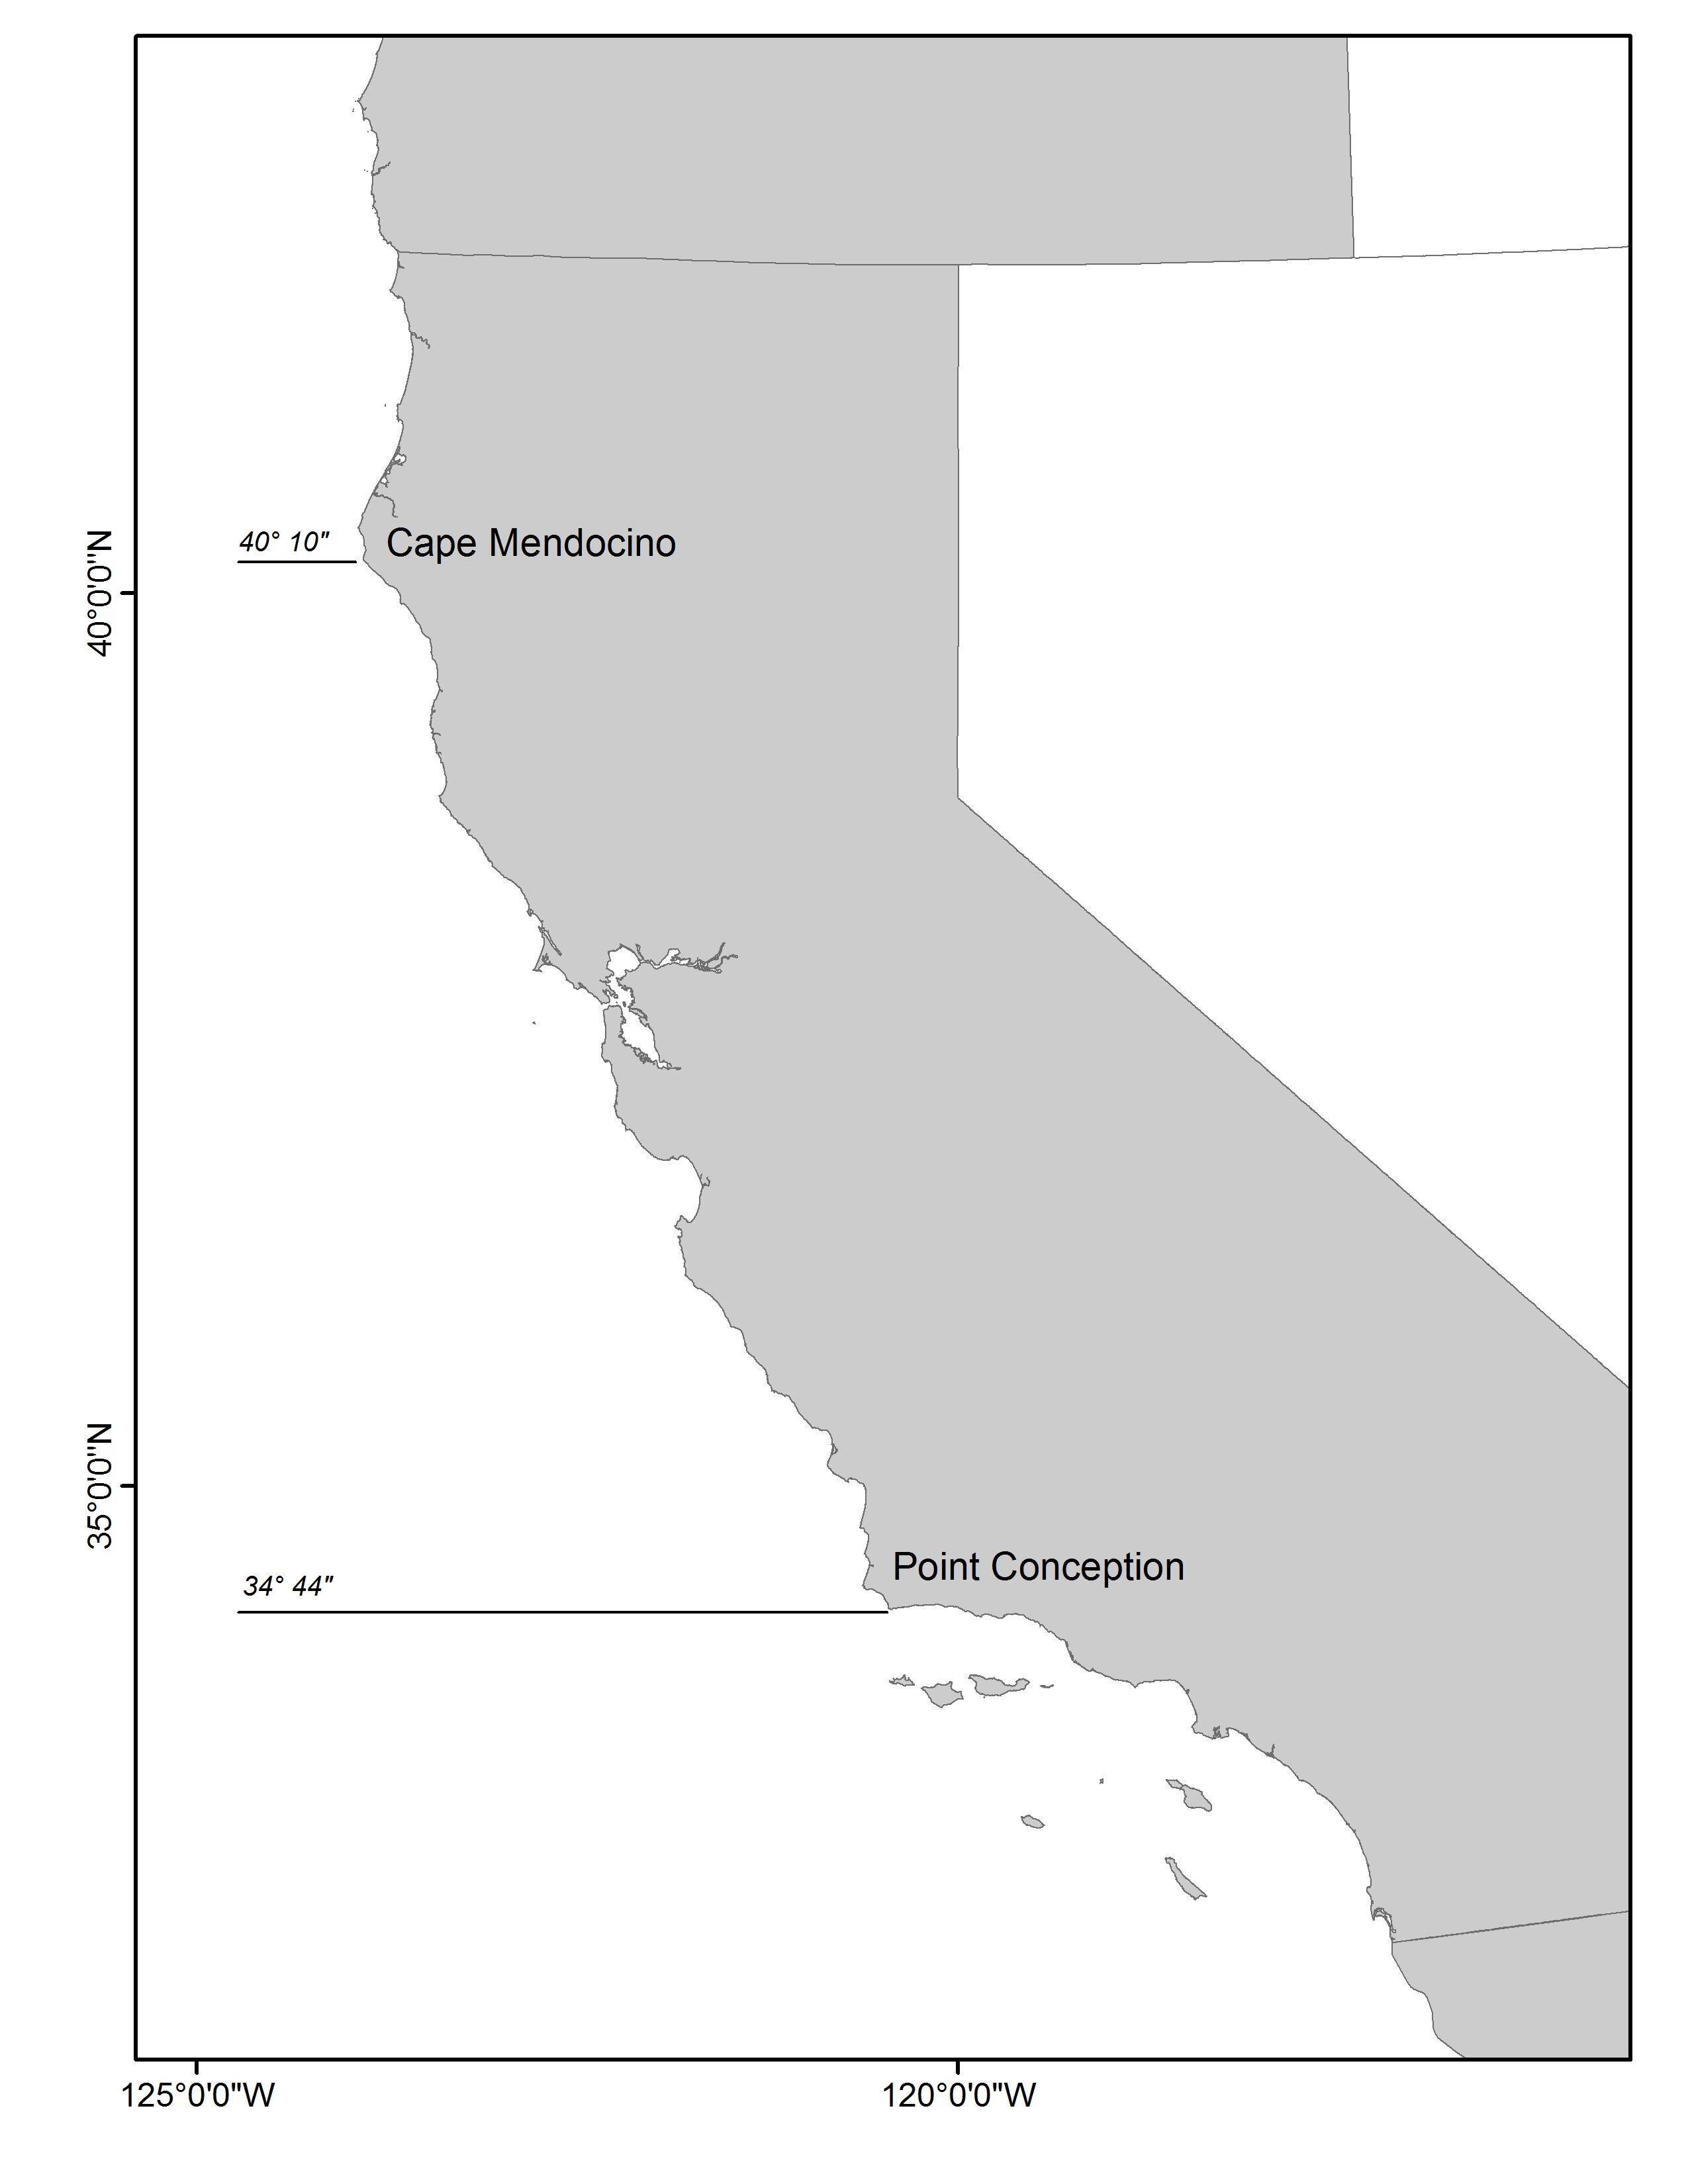
\includegraphics{Figures/assess_region_map.png}
\caption{Map showing the management area for gopher and black-and-yellow
rockfish from Cape Mendocino to the U.S.-Mexico border.
\label{fig:assess_region_map1}}
\end{figure}

\begin{figure}
\centering
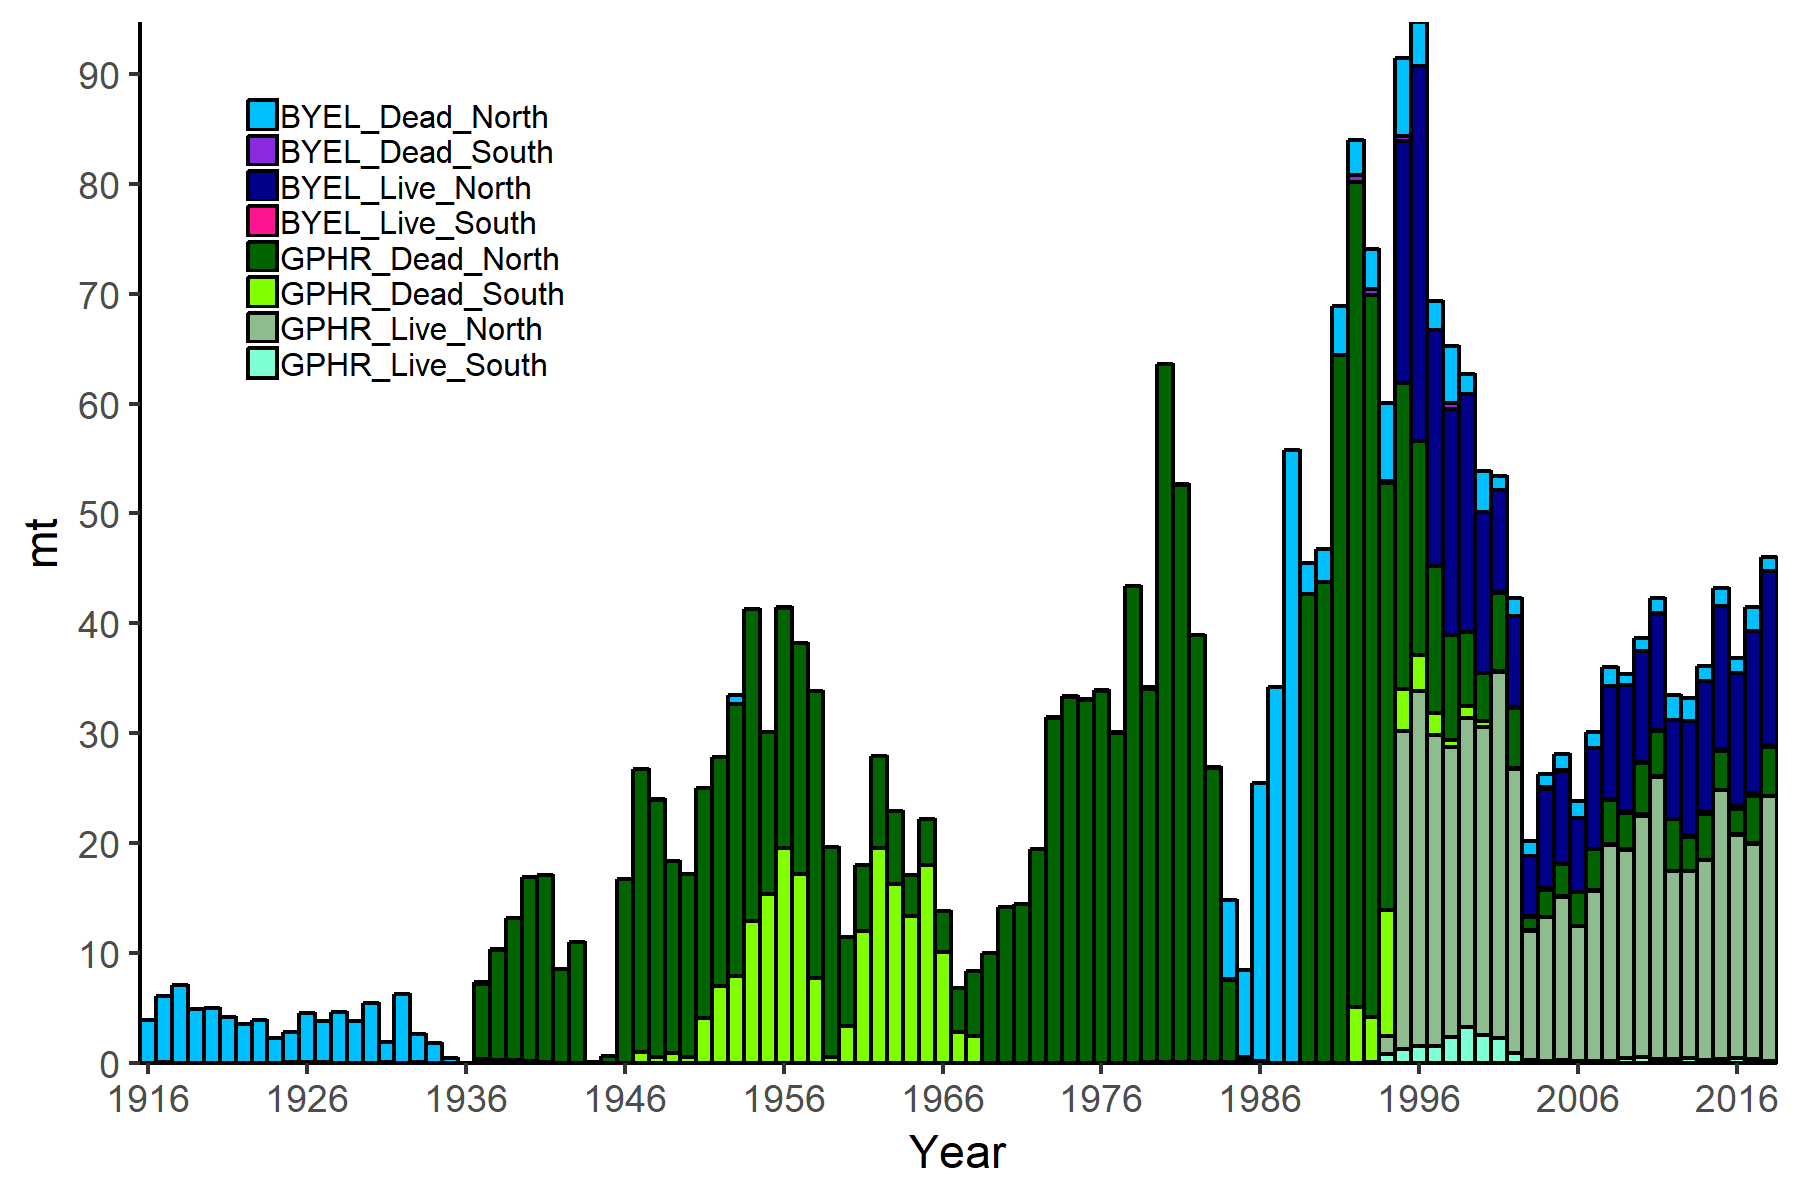
\includegraphics{Figures/Catches_livedeadNS_gby.png}
\caption{Commercial landings for gopher (GPHR) and black-and-yellow
(BYEL) rockfishes landed live and dead north and south of Point
Conception. All catch time series were combined for the assessment into
one commercial fleet. \label{fig:Catches_livedeadNS_gby}}
\end{figure}

\begin{figure}
\centering
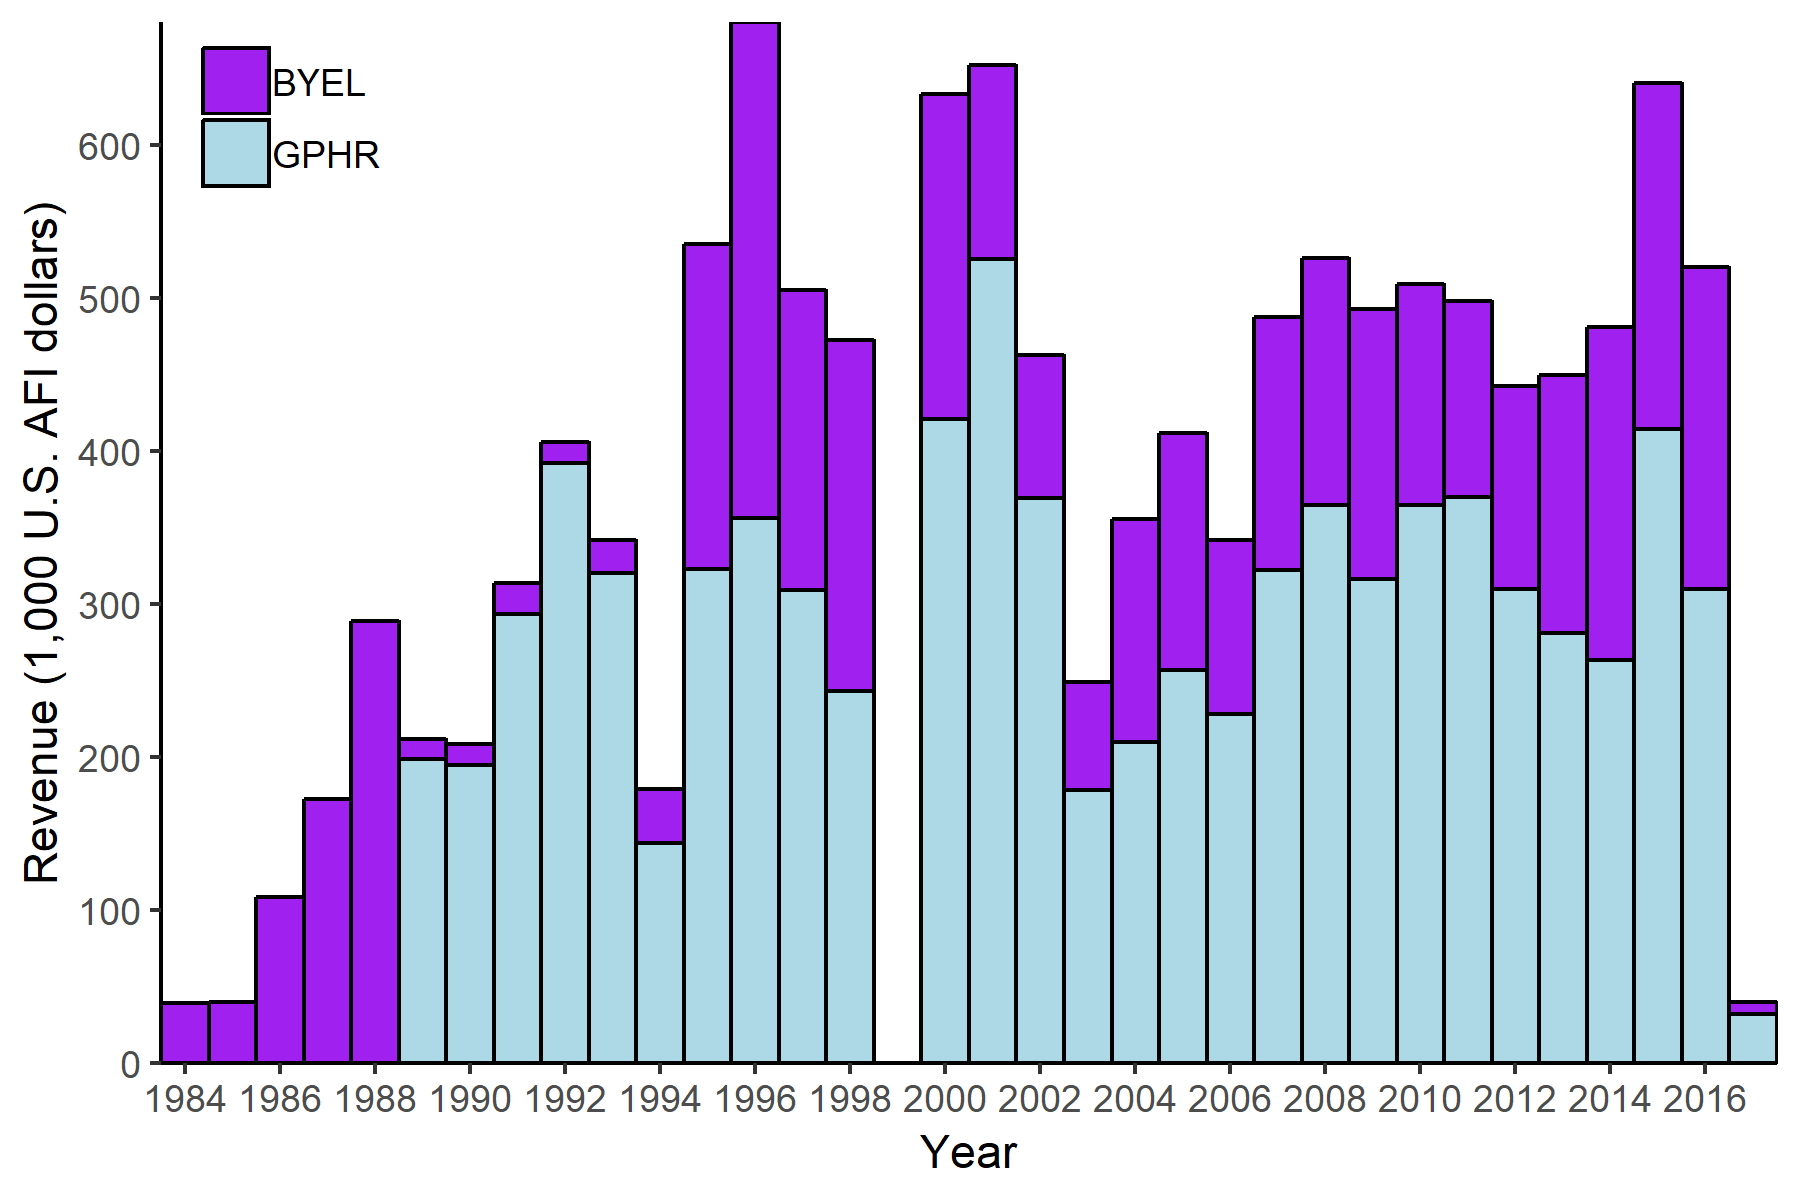
\includegraphics{Figures/GBY_revenue.png}
\caption{Annual ex-vessel revenue, adjusted for inflation (AFI) in
thousands of dollars for gopher and black-and-yellow rockfish.
\label{fig:GBY_revenue}}
\end{figure}

\begin{figure}
\centering
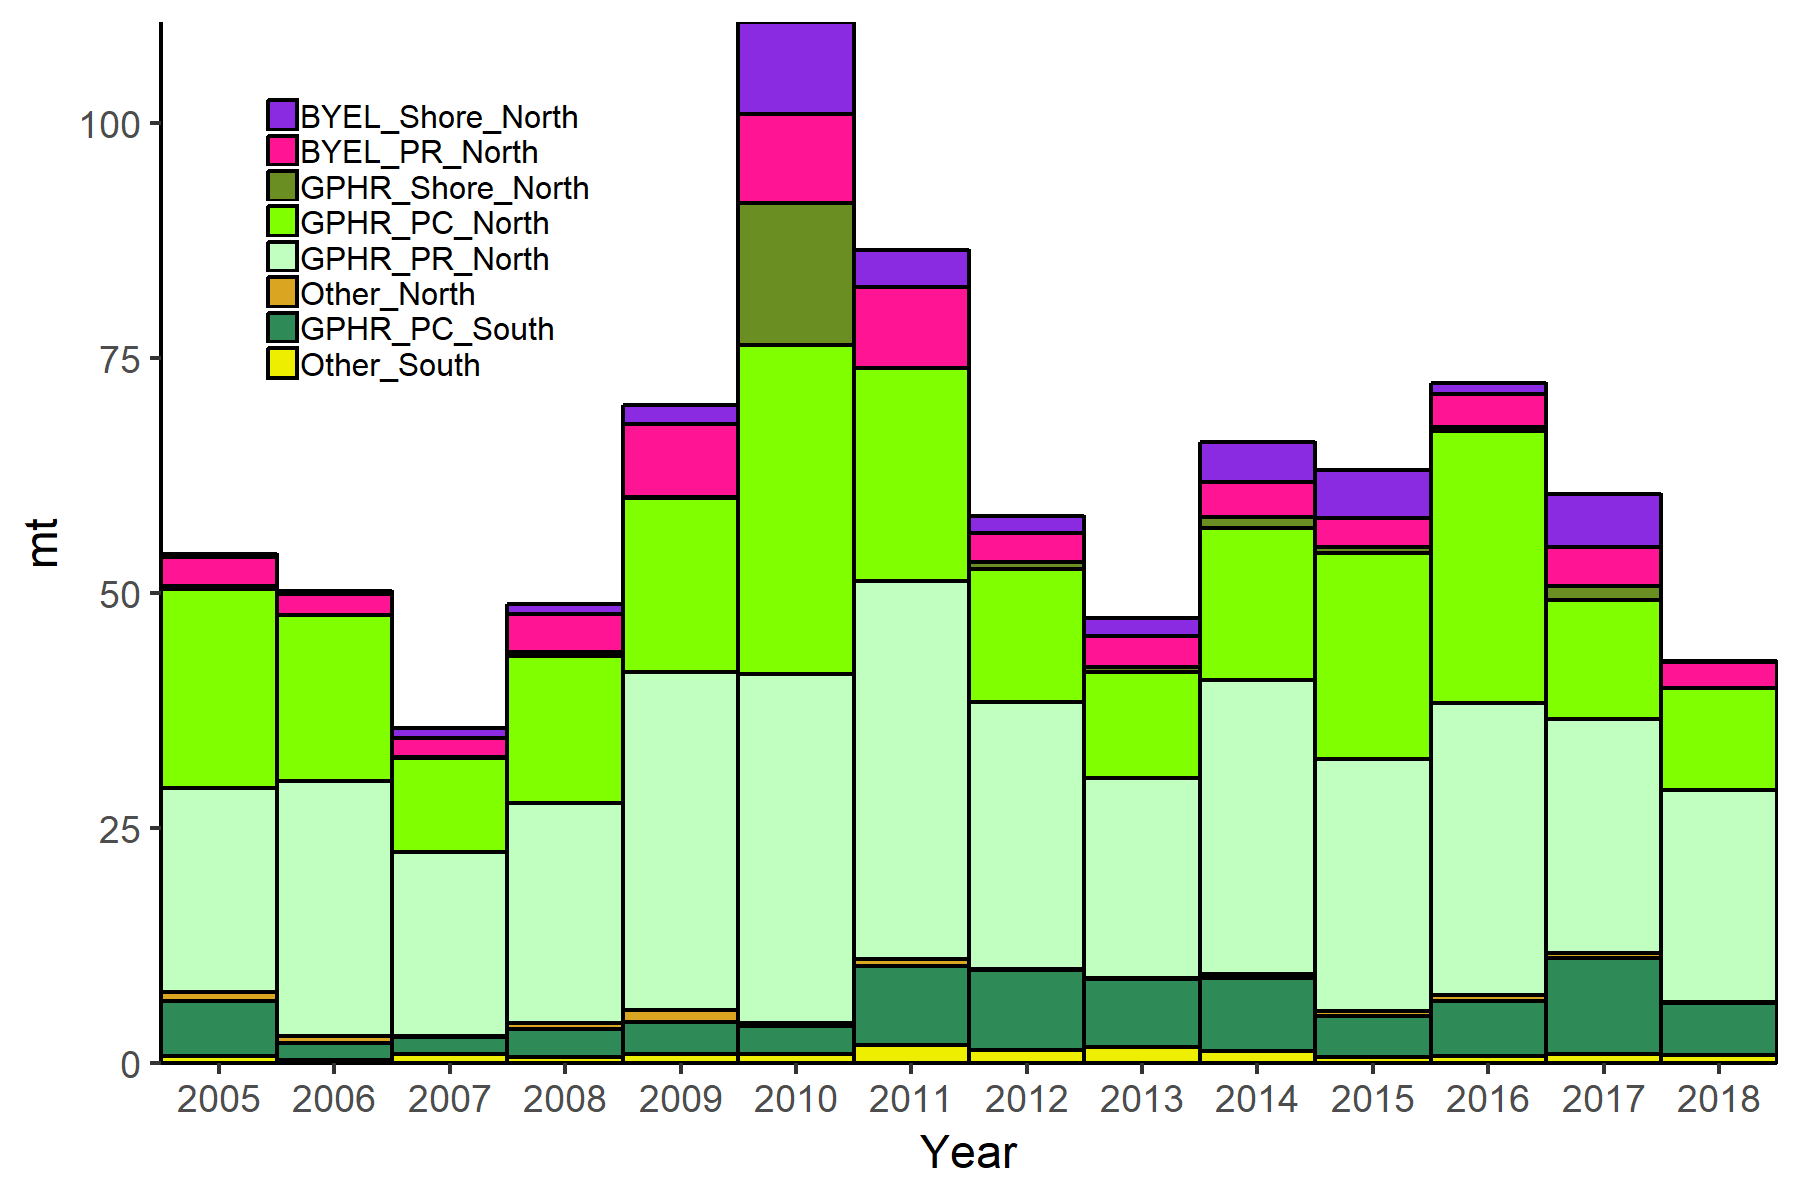
\includegraphics{Figures/CRFS_totalmort_gby.png}
\caption{Recreational total mortality for gopher rockfish (GPHR) and
black-and-yellow (BYEL) rockfish from the CDFW CRFS sampling era by mode
and split north and south of Point Conception. \label{fig:CFRS_catches}}
\end{figure}

\begin{figure}
\centering
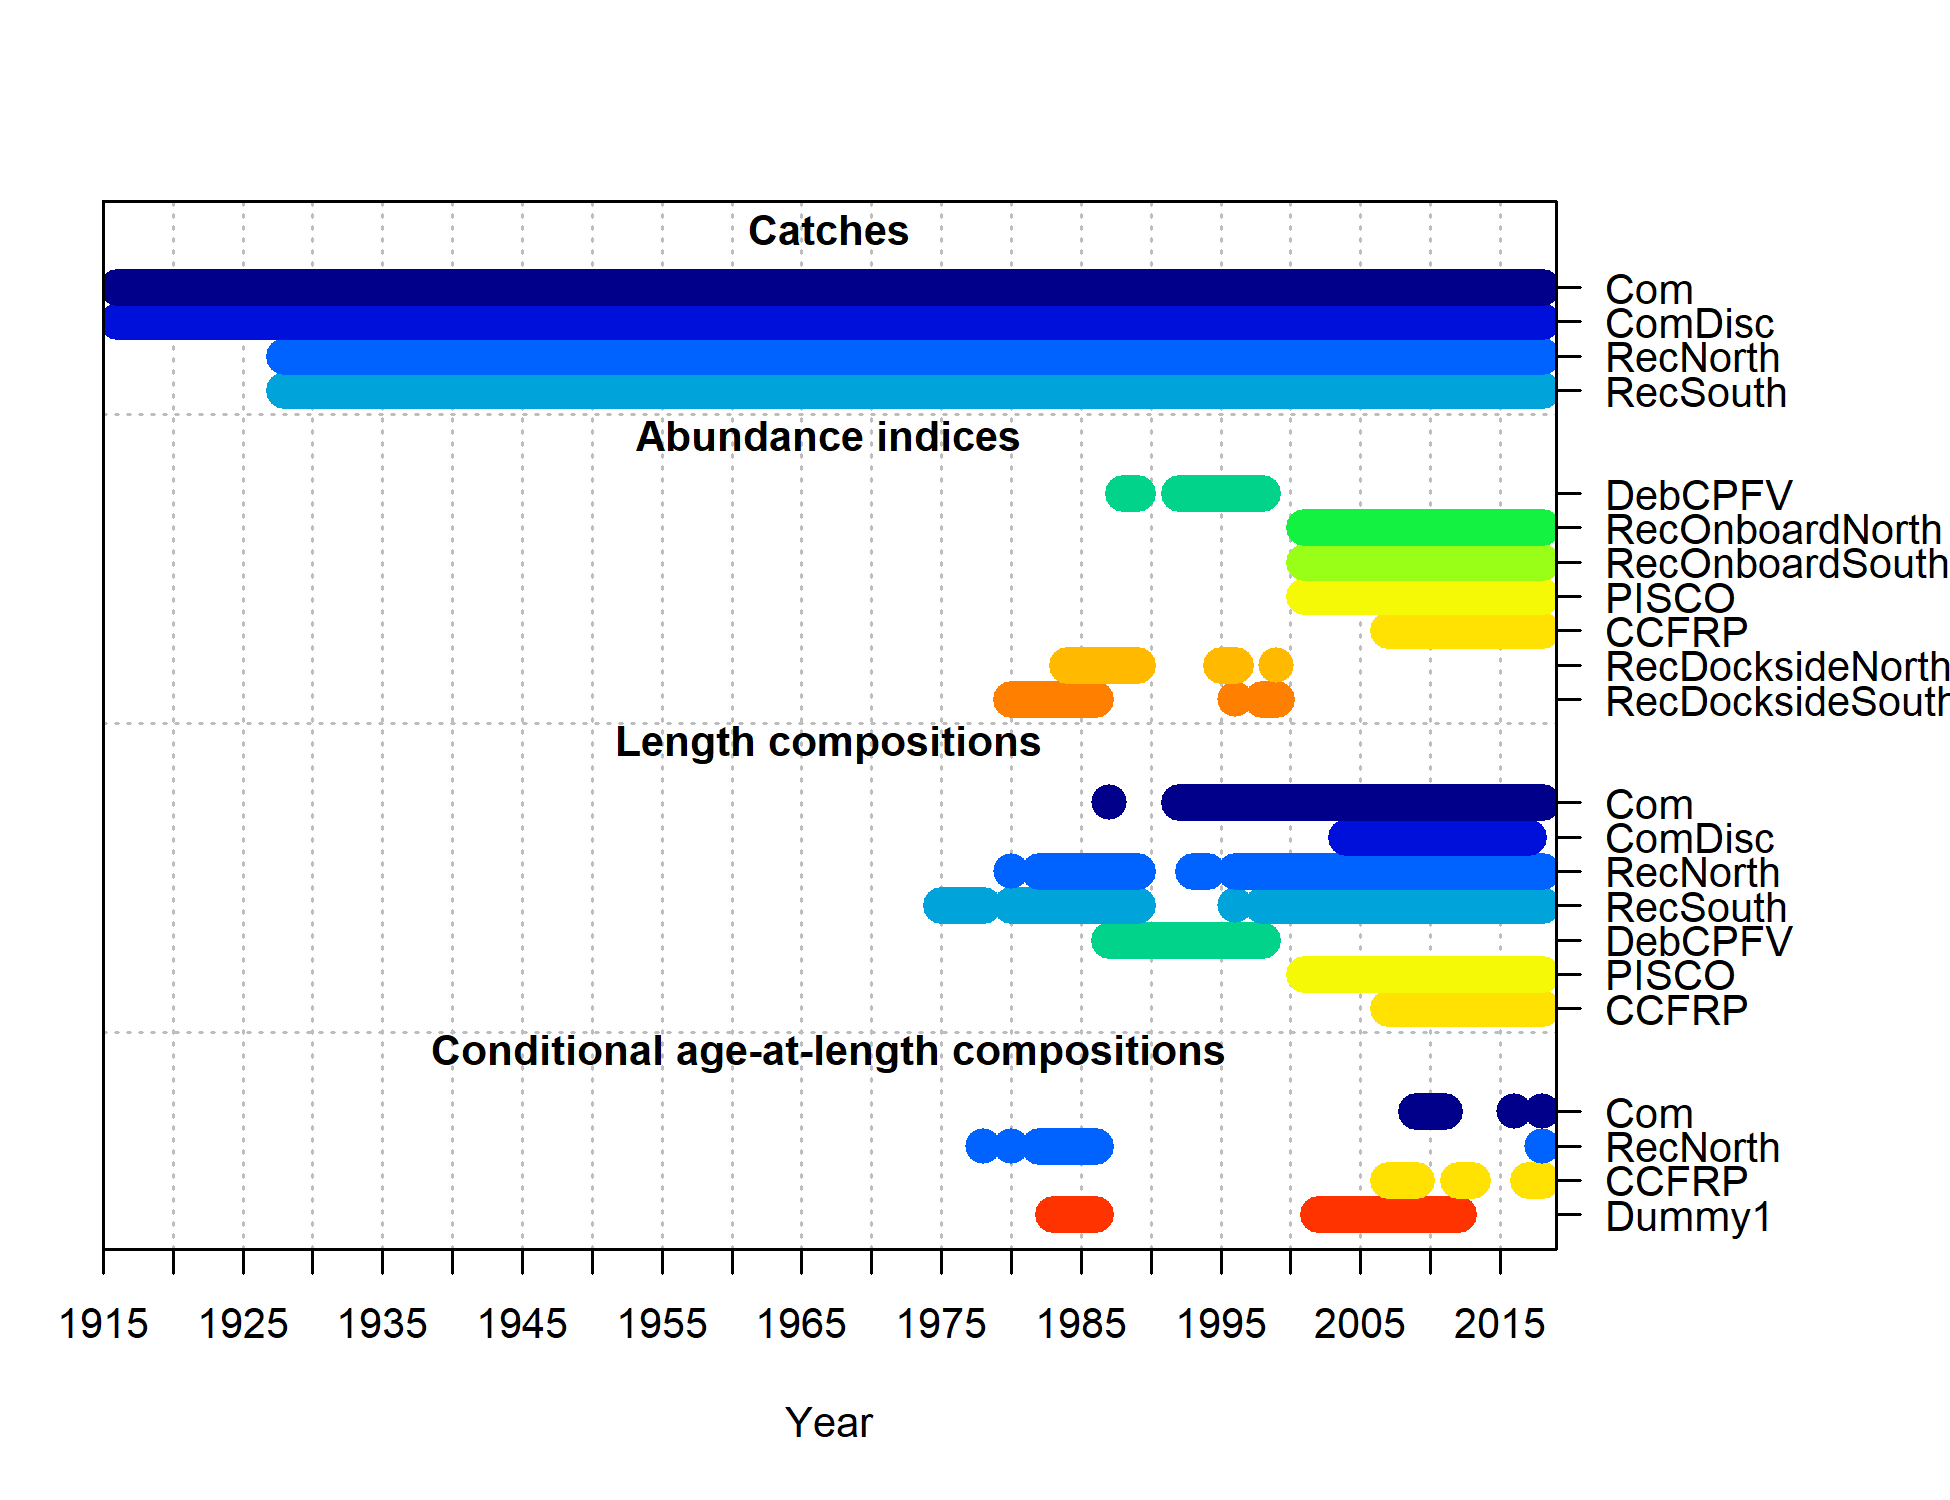
\includegraphics{r4ss/plots_mod1/data_plot.png}
\caption{Summary of data sources used in the model.
\label{fig:data_plot}}
\end{figure}

\begin{figure}
\centering
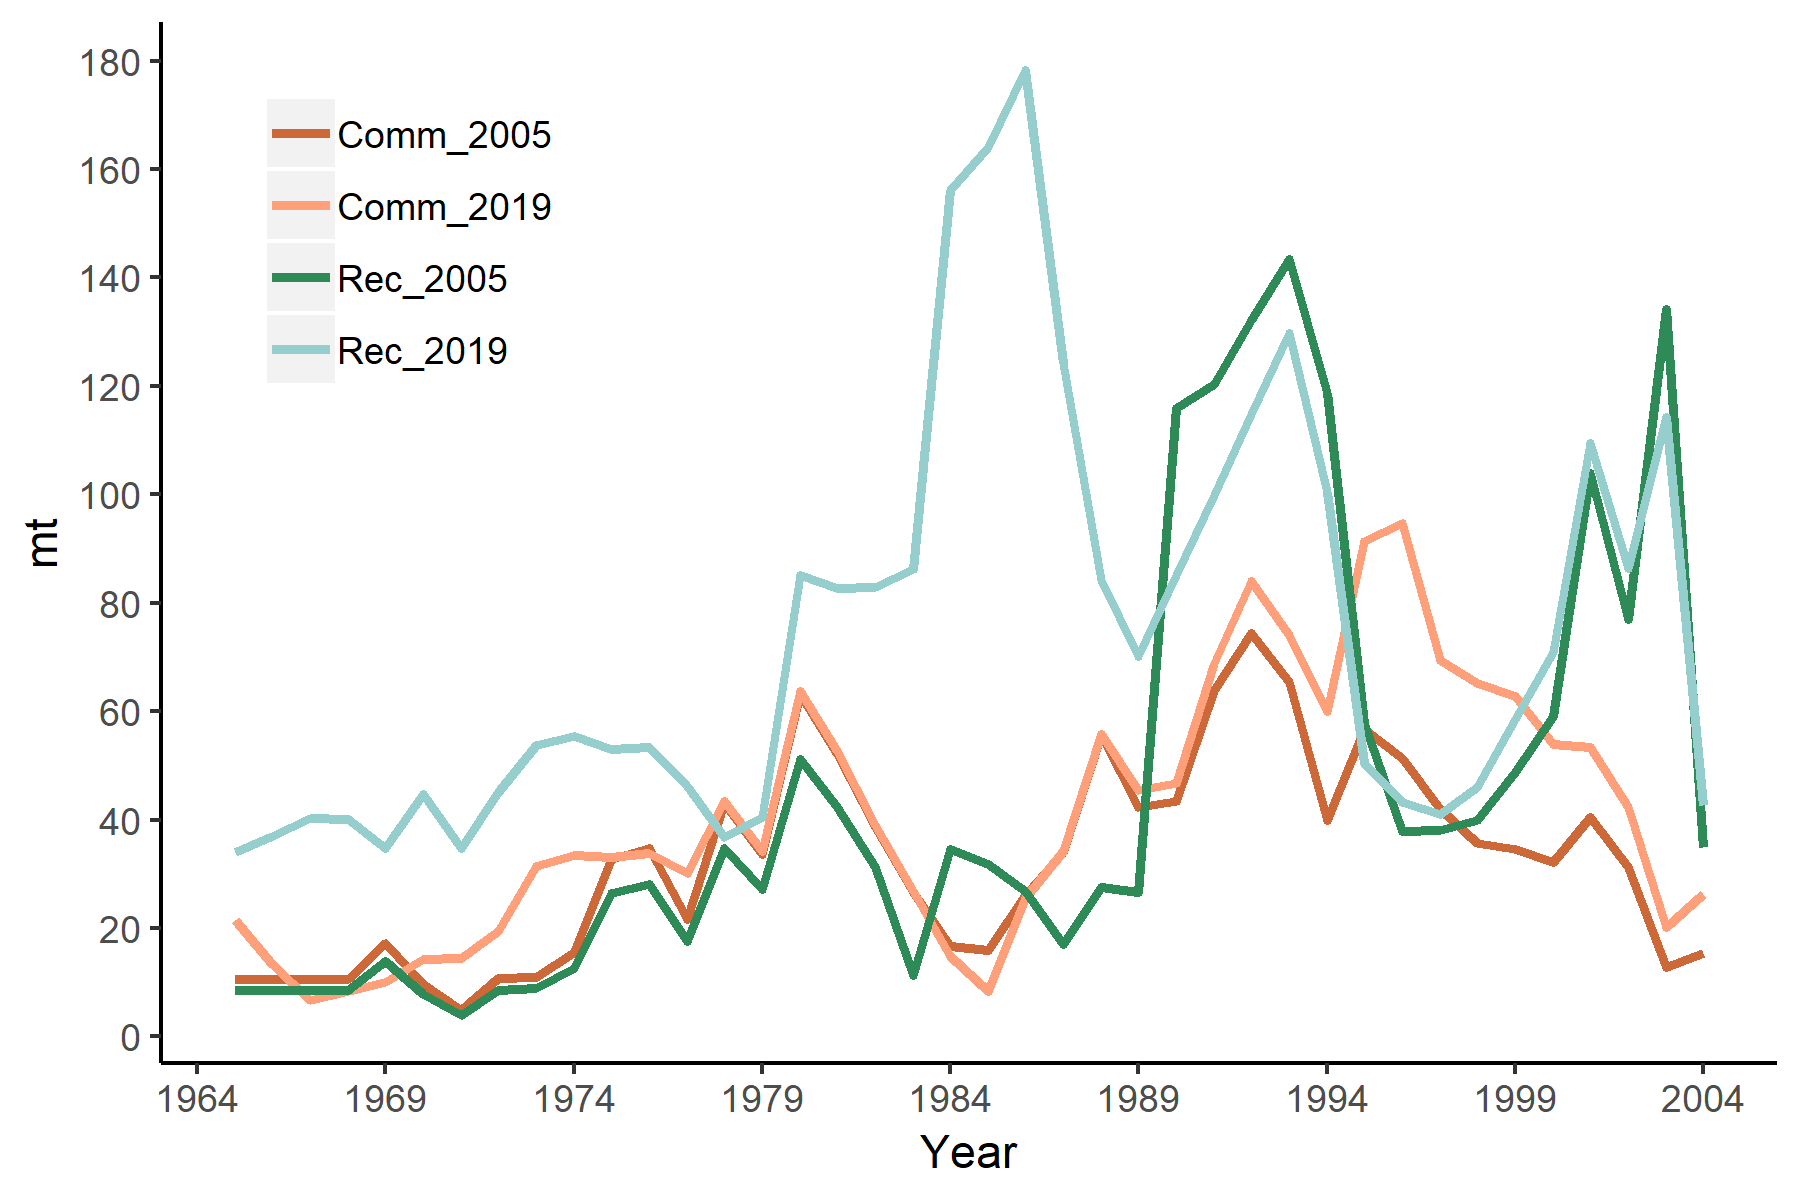
\includegraphics{Figures/assessment_compare.png}
\caption{Comparison of the recreational and commercial fishery landings
from the 2005 assessment to this 2019 assessment. Note that the 2019
assessment includes both gopher and black-and-yellow rockfish where the
2005 assessment represents gopher rockfish only. The 2005 assessment
also did not include landings from south of Point Conception.
\label{fig:Assessment_compare}}
\end{figure}

\begin{figure}
\centering
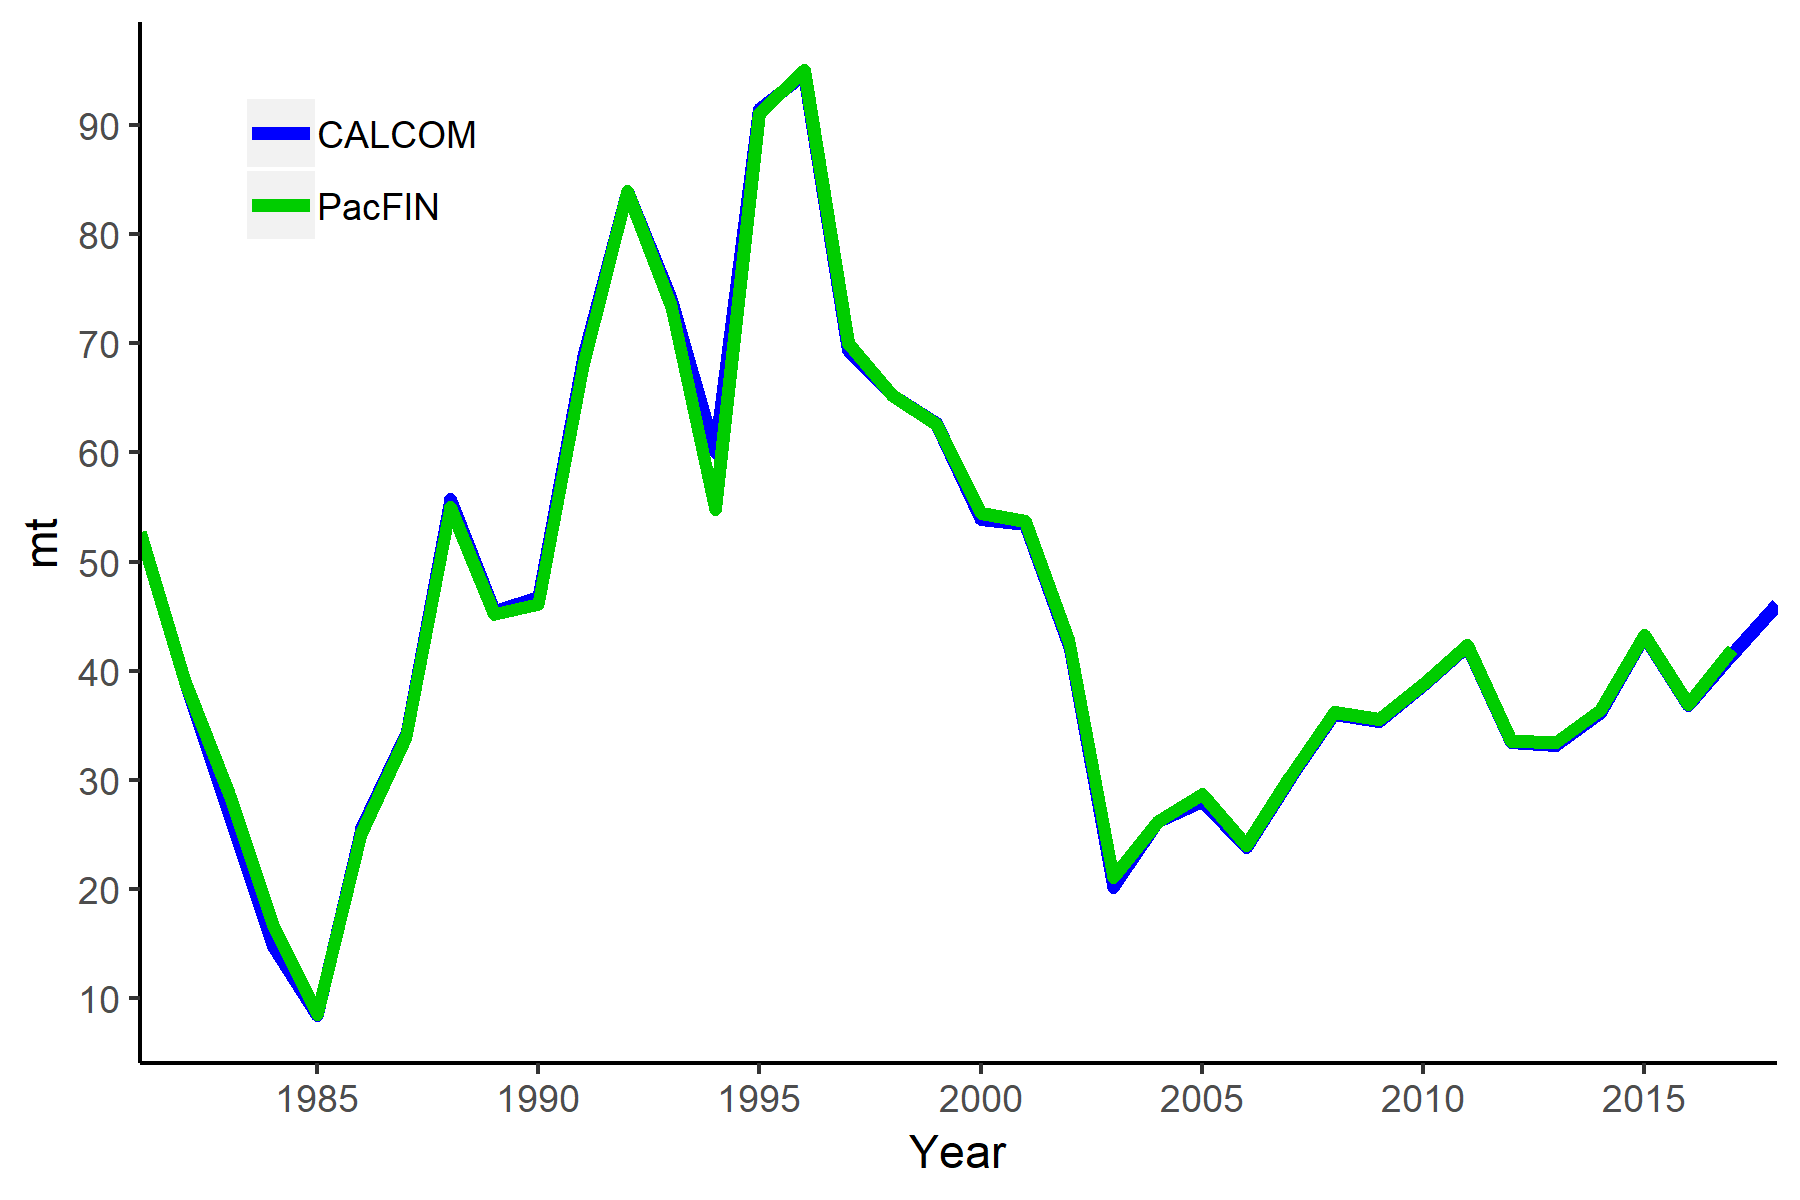
\includegraphics{Figures/Calcom_vs_Pacfin.png}
\caption{Commercial landings estimates from CALCOM add PacFIN.
\label{fig:Calcom_vs_Pacfin}}
\end{figure}

\begin{figure}
\centering
\includegraphics{Figures/Calcom_vs_pacfin_lengths.png}
\caption{Percent differences in the expanded length compositions by year
from CALCOM and PacFIN. The same market categories were used for each
dataset, but each database was subject to further independent filtering
criteria and expansion algorithms. \label{fig:Calcom_vs_pacfin_lengths}}
\end{figure}

\begin{figure}
\centering
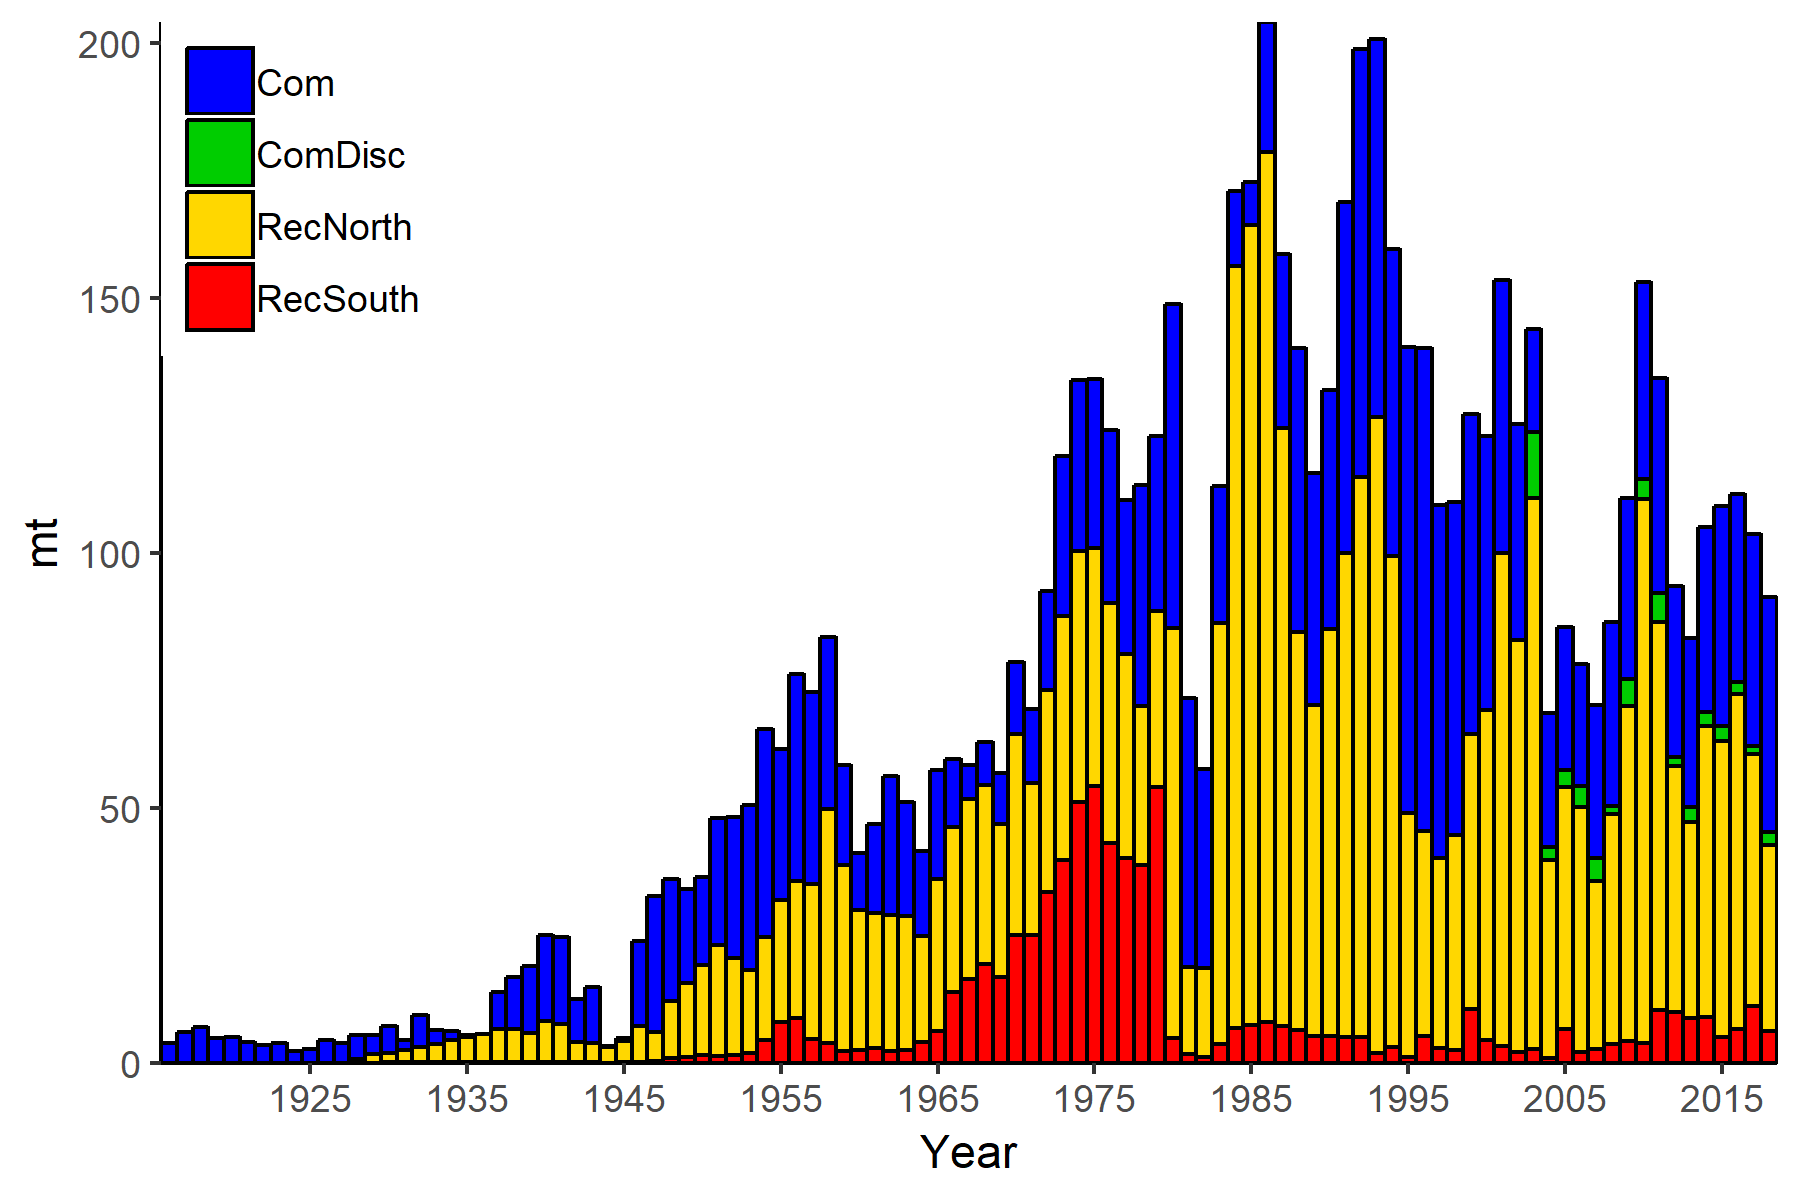
\includegraphics{Figures/Catches_original.png}
\caption{Commercial and recreational landings estimates prior to any
data modification or interpolation to the recreational catches or
hindcasting of commercial discards. \label{fig:Catches_original}}
\end{figure}

\begin{figure}
\centering
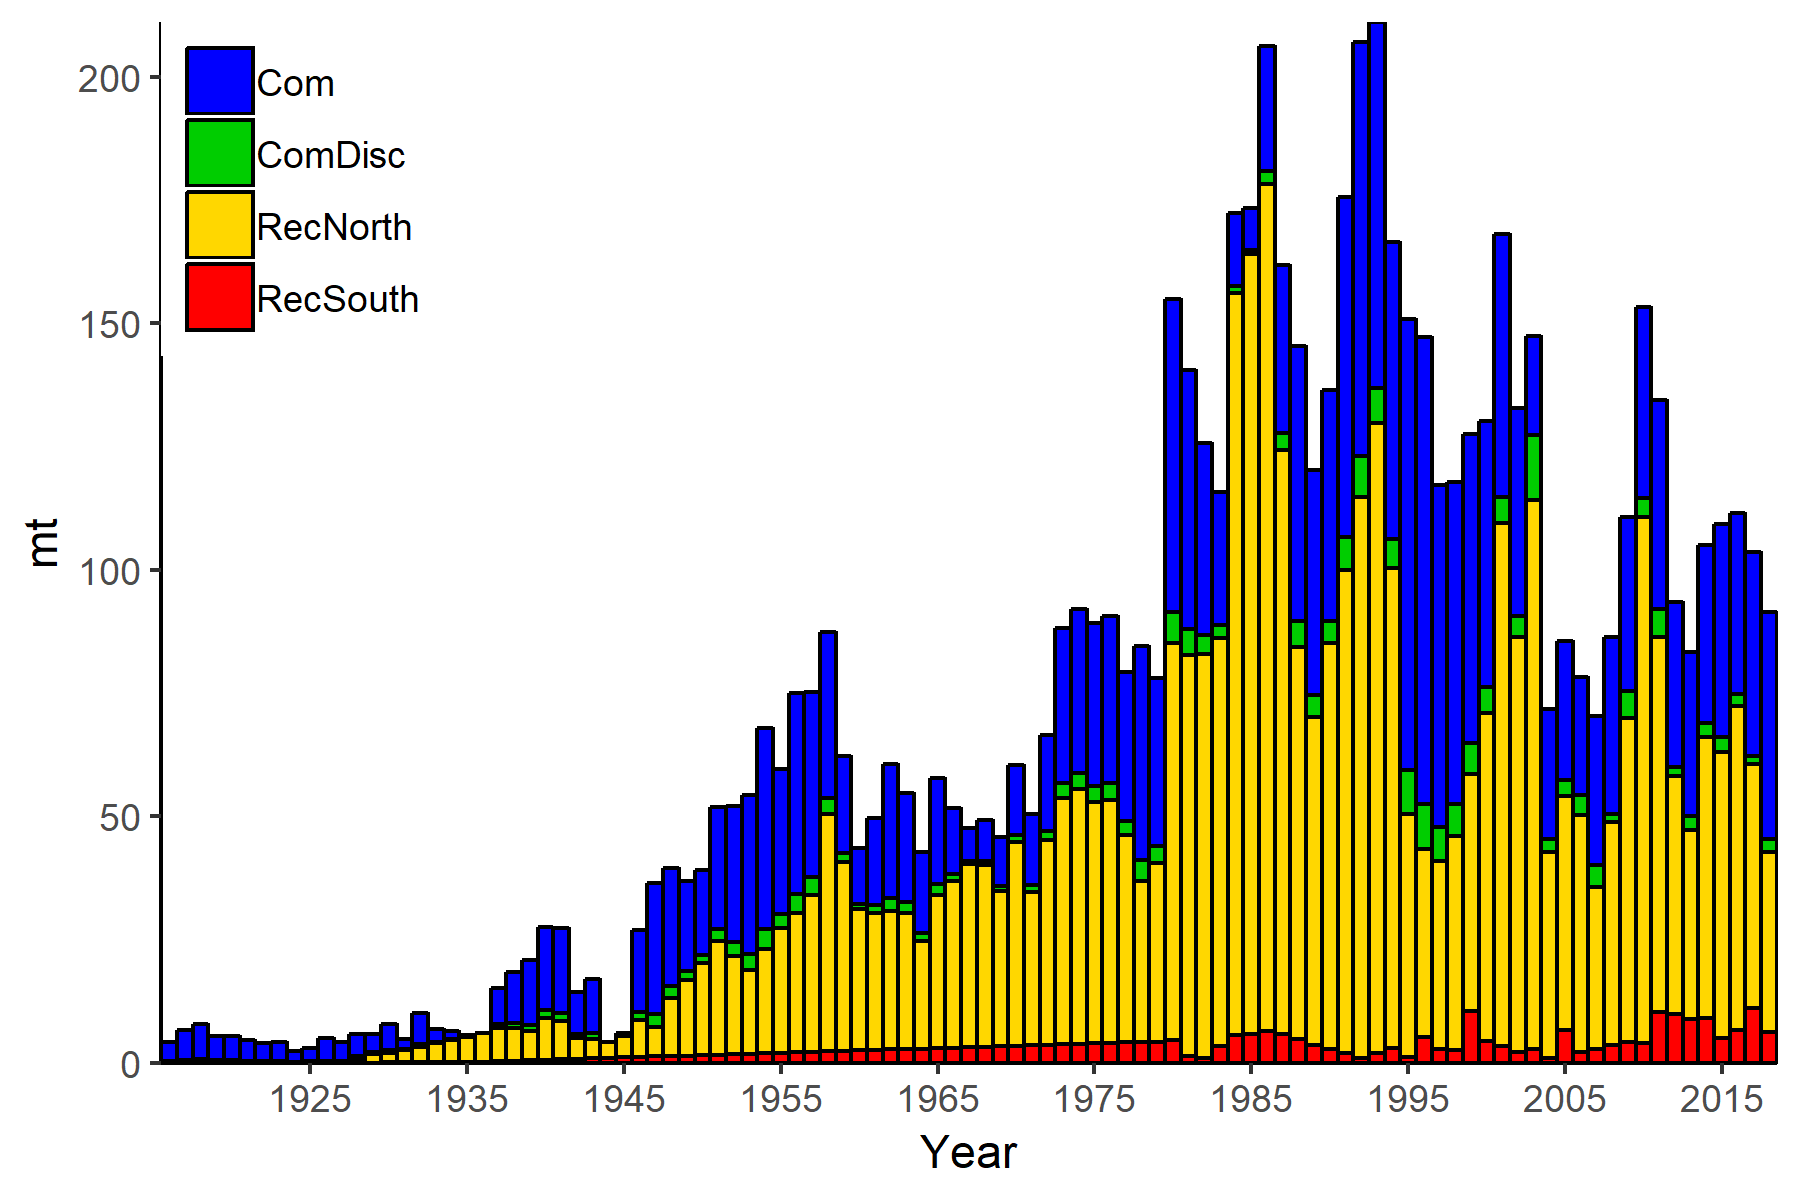
\includegraphics{Figures/Catches_alternate.png}
\caption{Commercial and recreational landings estimates after data
modification and interpolations were made to the recreational catches
and commercial discards. \label{fig:Catches_alternate}}
\end{figure}

\FloatBarrier

\begin{figure}
\centering
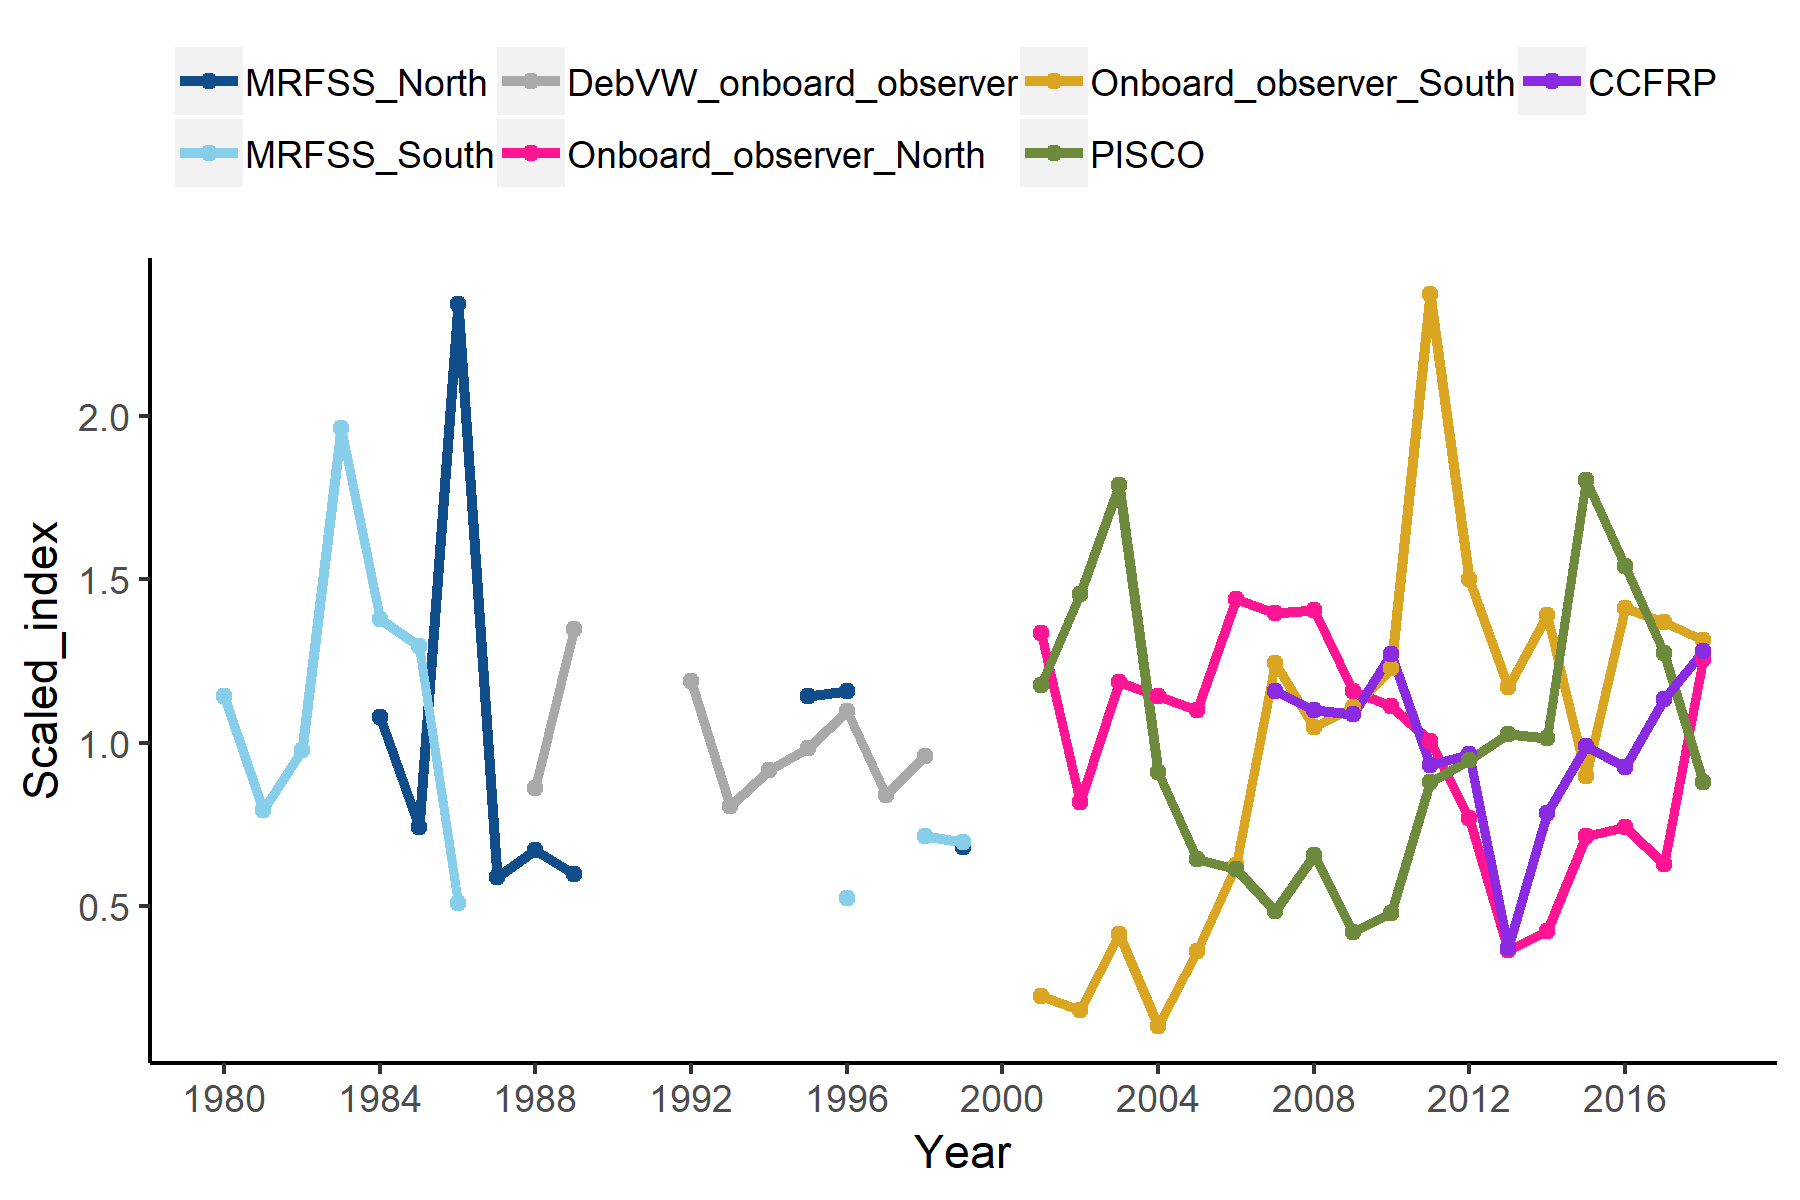
\includegraphics{Figures/All_index_compare.png}
\caption{Comparison of all indices of abundance (scaled to their means).
\label{fig:All_index_compare}}
\end{figure}

\begin{figure}
\centering
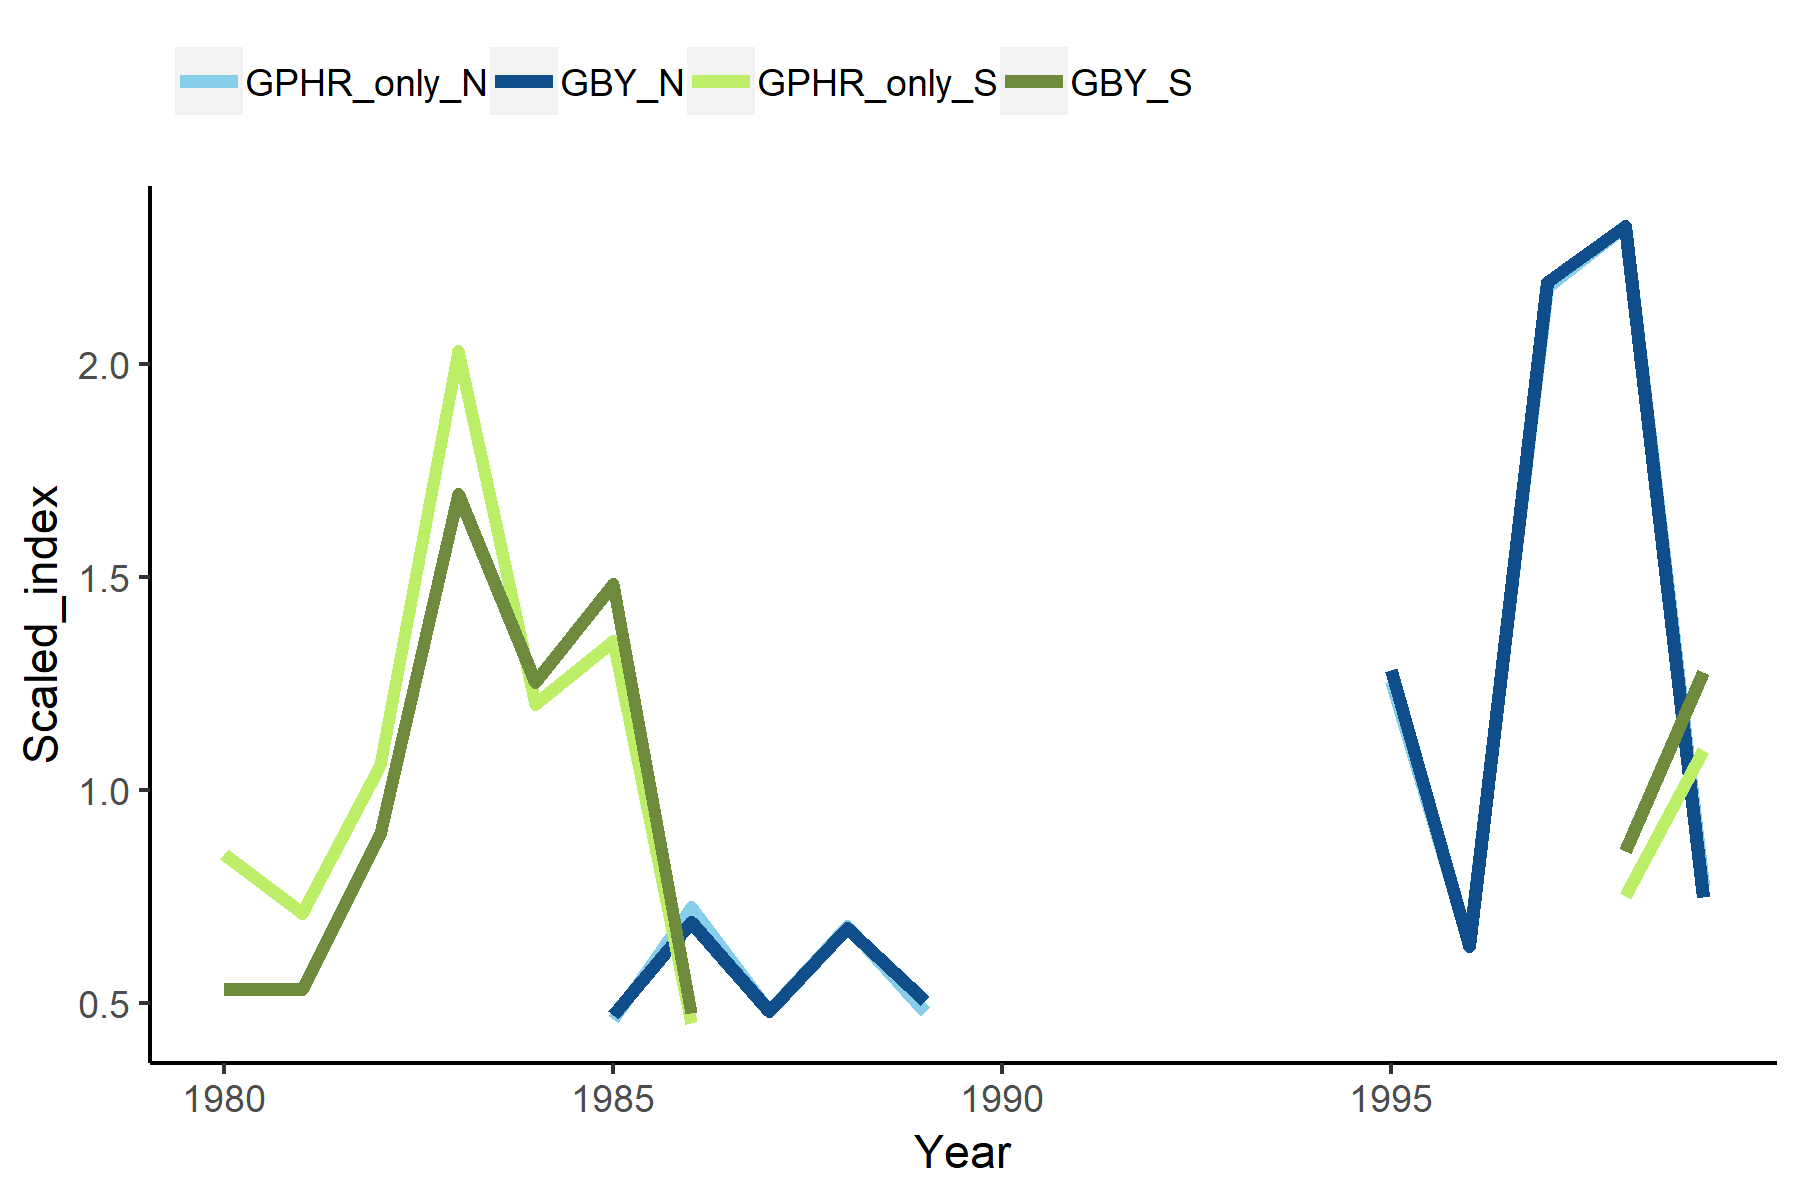
\includegraphics{Figures/MRFSS_index_compare.png}
\caption{Comparison of indices of abundance (scaled to their means) for
the MRFSS dockside CPFV survey between a gopher-only and GBYR complex
index for north and south of Point Conception.
\label{fig:MRFSS_index_compare}}
\end{figure}

\begin{figure}
\centering
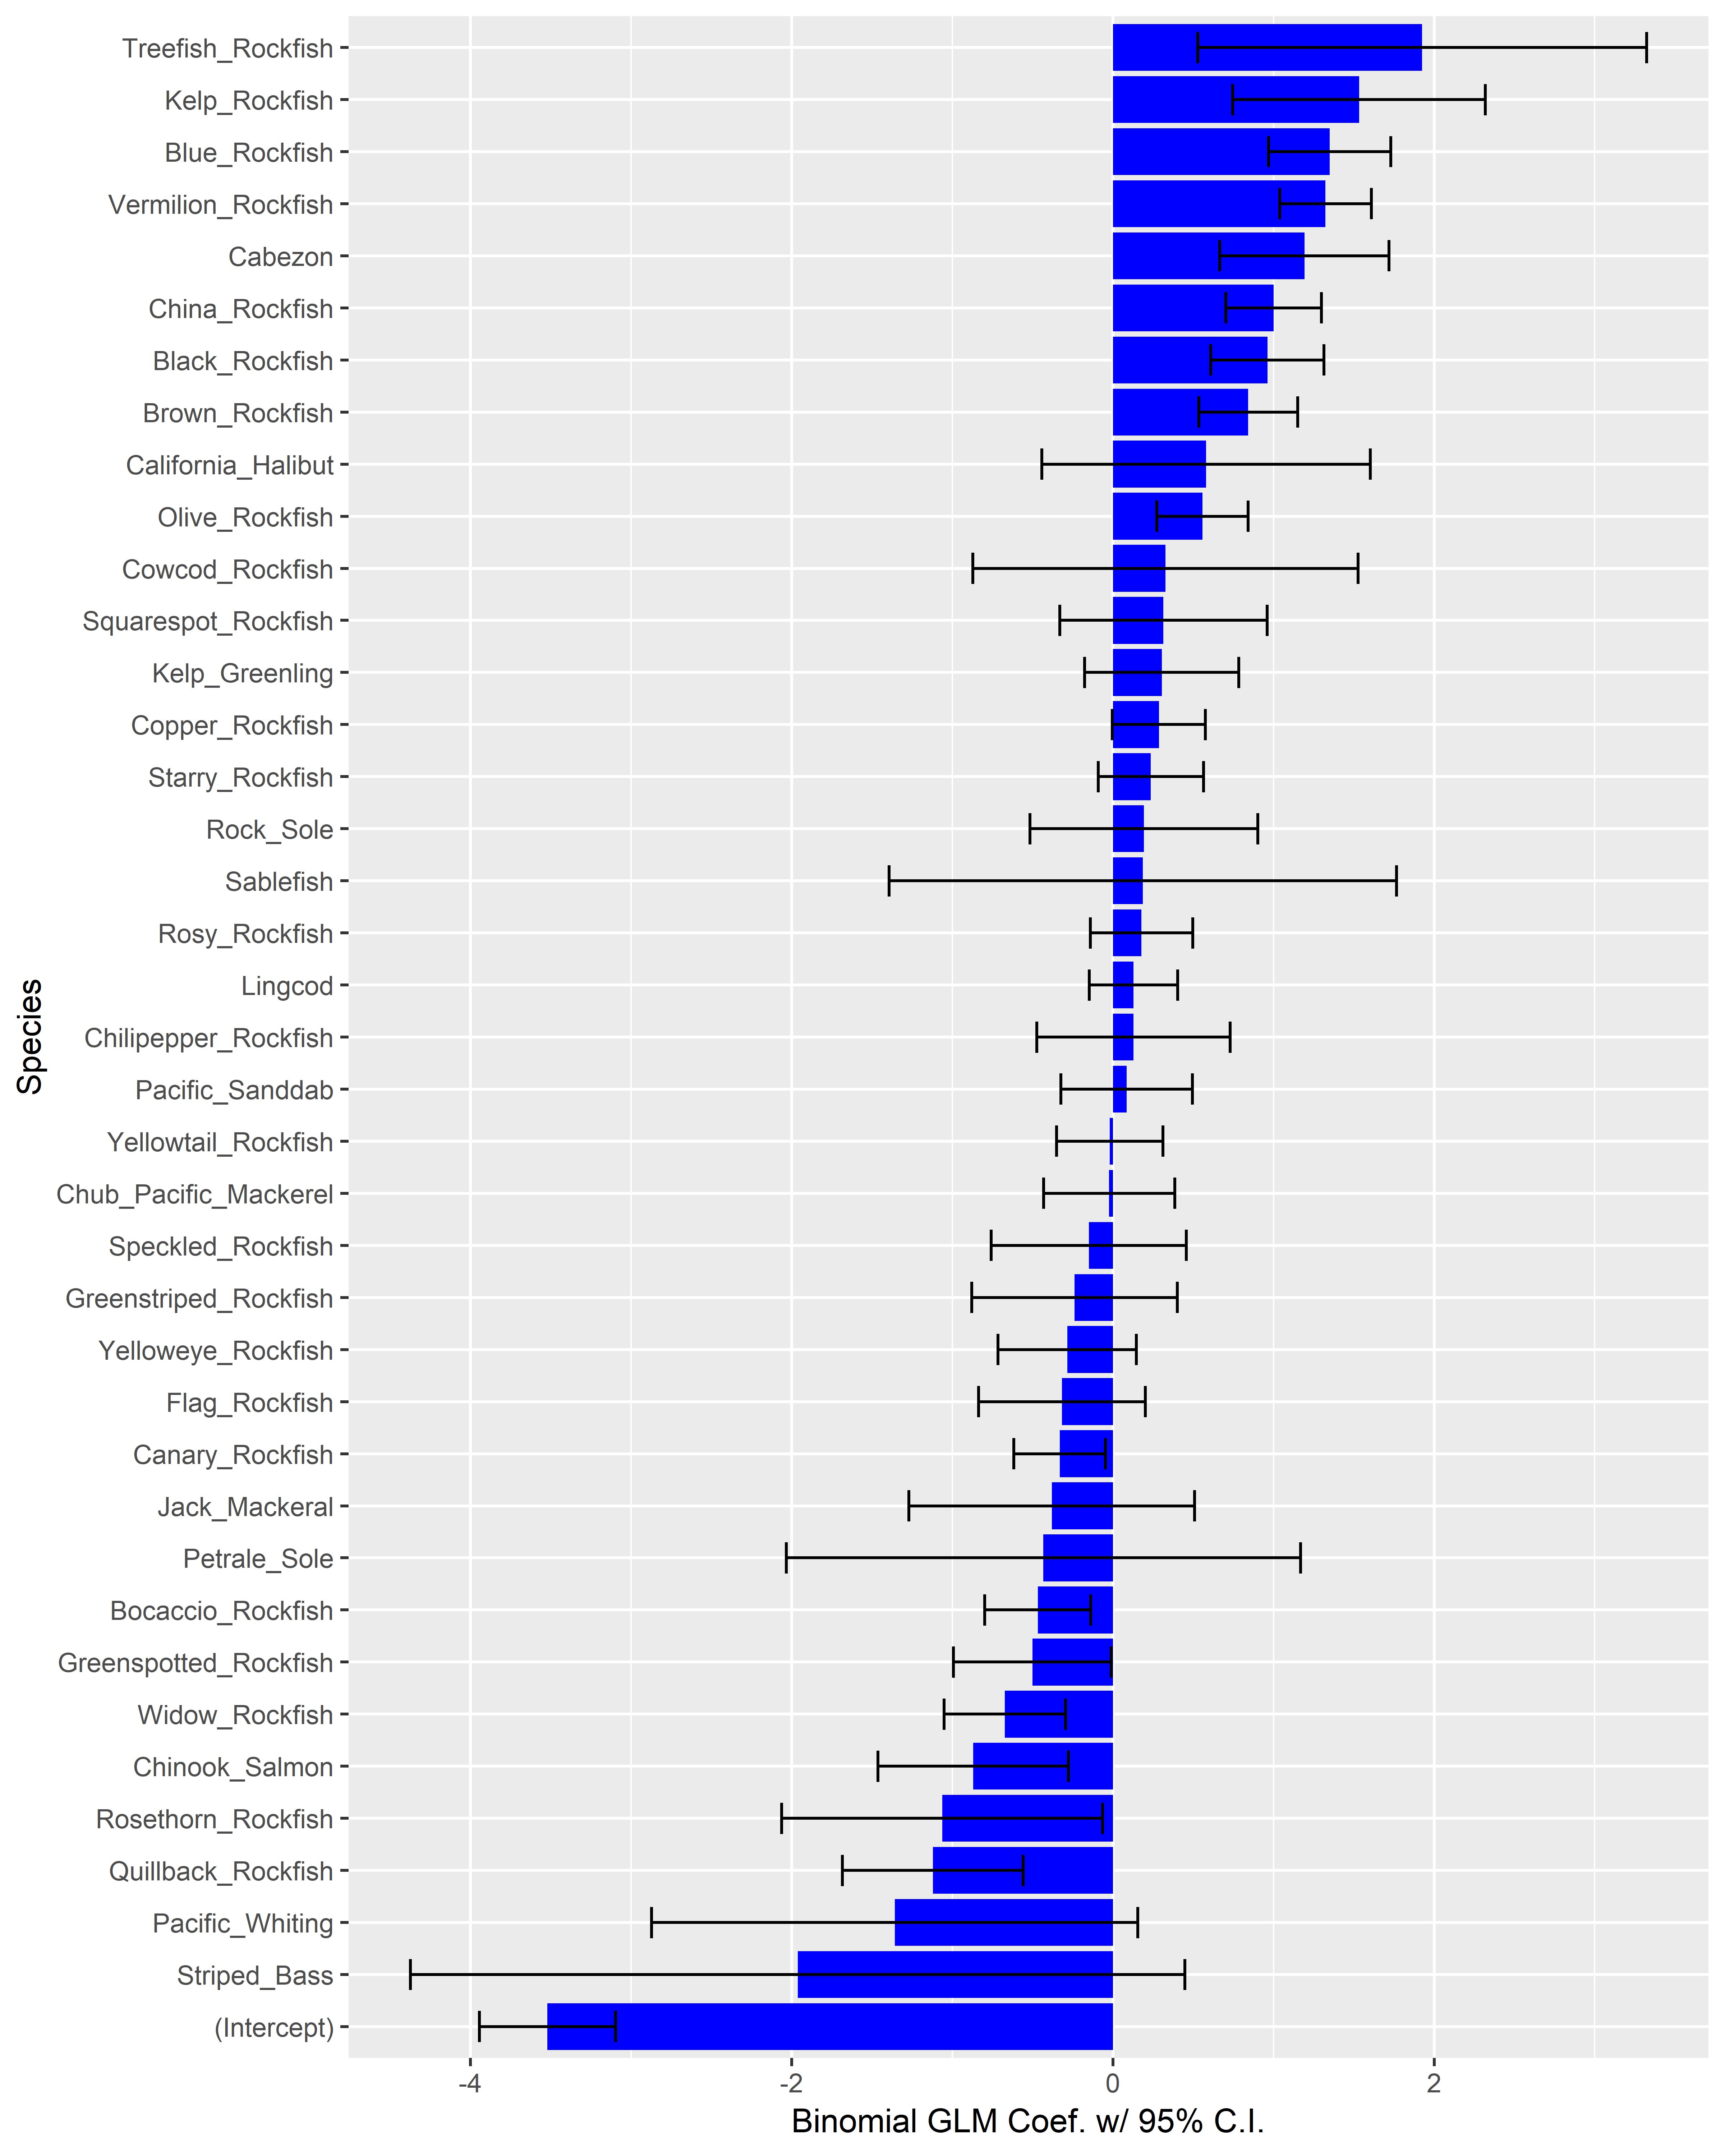
\includegraphics{Figures/Fleet10_SM_filter.png}
\caption{Species coefficients from the binomial GLM for presence/absence
of GBYR in the Marine Recreational Fisheries Statistics Survey (MRFSS)
CPFV mode dockside survey data set north of Point Conception. Horizontal
bars are 95\% confidence intervals. \label{fig:Fleet10_SM_filter}}
\end{figure}

\begin{figure}
\centering

\includegraphics{Figures/MRFSS_index_N_SM_falsepos.png}
\caption{Comparisons of the indices of abundance for GBYR north of Point
Conception from the MRFSS dockside CPVS survey that either include of
exclude the trips identified as false positives from the
Stephens-MacCall filter. \label{fig:MRFSS_index_N_SM_falsepos}}
\end{figure}

\begin{figure}
\centering
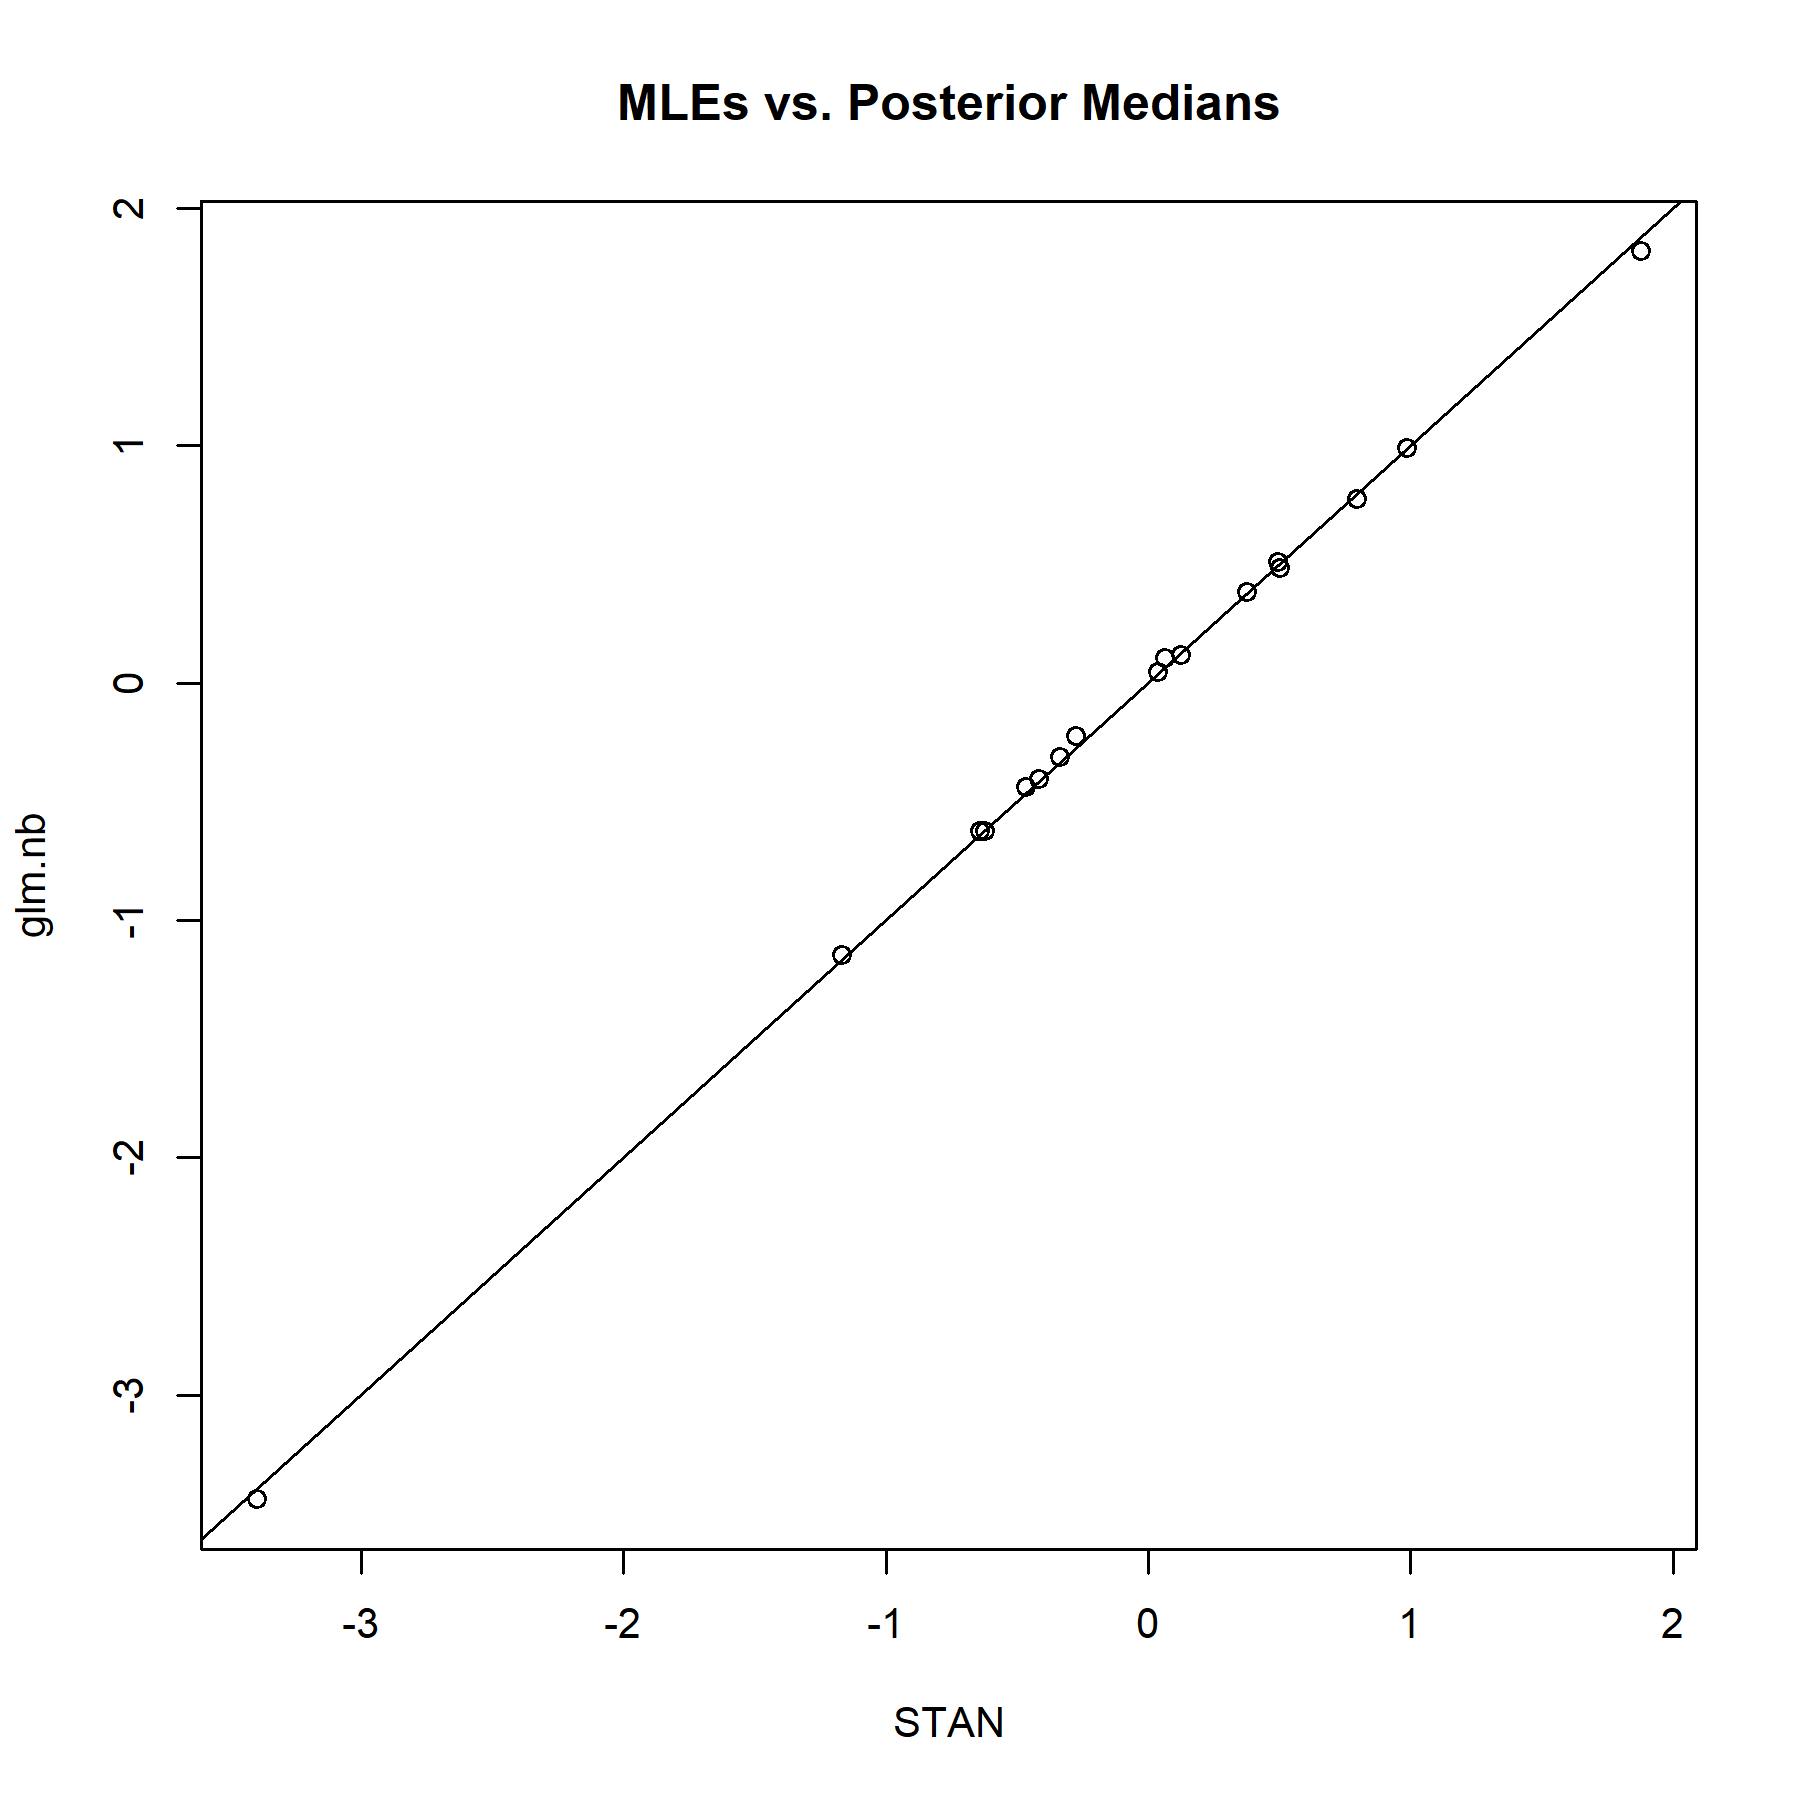
\includegraphics{Figures/Fleet10_MLE_stan.png}
\caption{Comparison of negative binomial predictions (CPUE) to observed
means in each stratum (year) MRFSS CPFV dockside index north of Point
Conception. The 1:1 plot is for reference. \label{fig:Fleet10_MLE_stan}}
\end{figure}

\begin{figure}
\centering
\includegraphics{Figures/Fleet10_prop_zero_STAN.png}
\caption{Posterior predictive distribution of the proportion of zero
observations in replicate data sets generated by the negative binomial
model for MRFSS dockside CPFV index north of Point Conception.
\label{fig:Fleet10_prop_zero_STAN}}
\end{figure}

\FloatBarrier

\begin{figure}
\centering
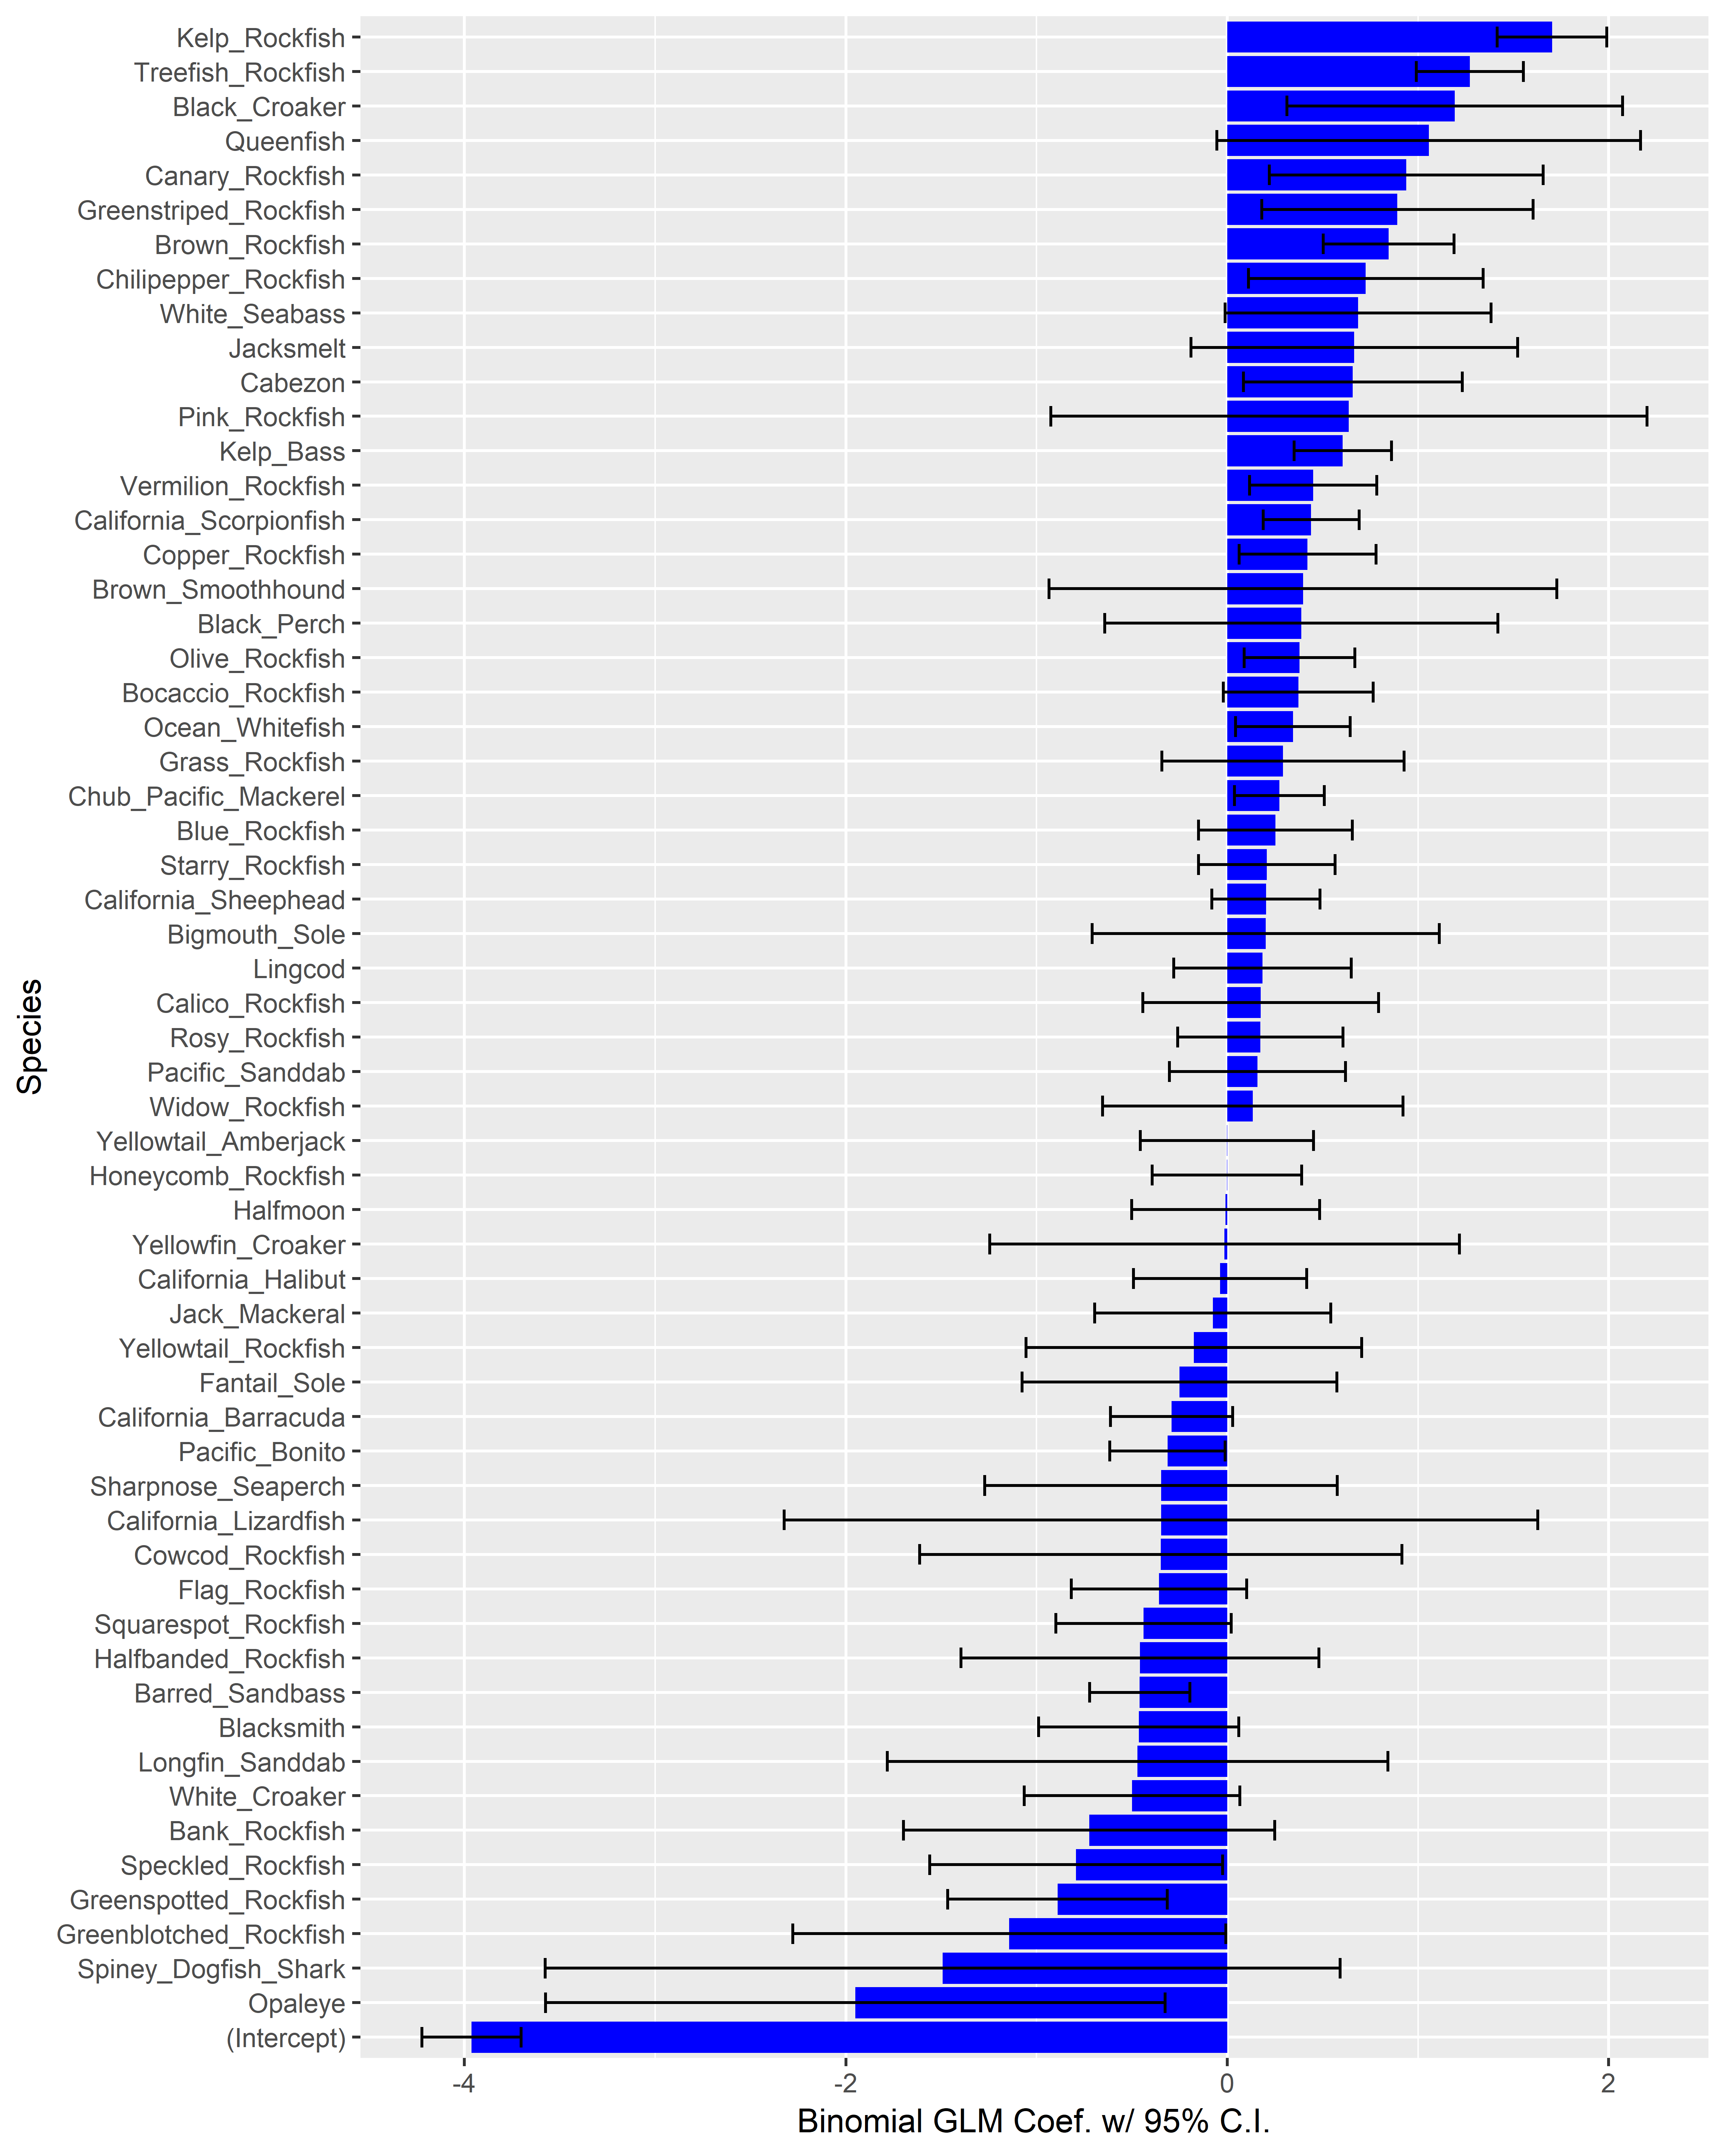
\includegraphics{Figures/Fleet11_SM_filter.png}
\caption{Species coefficients from the binomial GLM for presence/absence
of GBYR in the Marine Recreational Fisheries Statistics Survey (MRFSS)
CPFV mode dockside survey data set north of Point Conception. Horizontal
bars are 95\% confidence intervals. \label{fig:Fleet11_SM_filter}}
\end{figure}

\FloatBarrier
<!-- ********************************************************************** -->

\begin{figure}
\centering
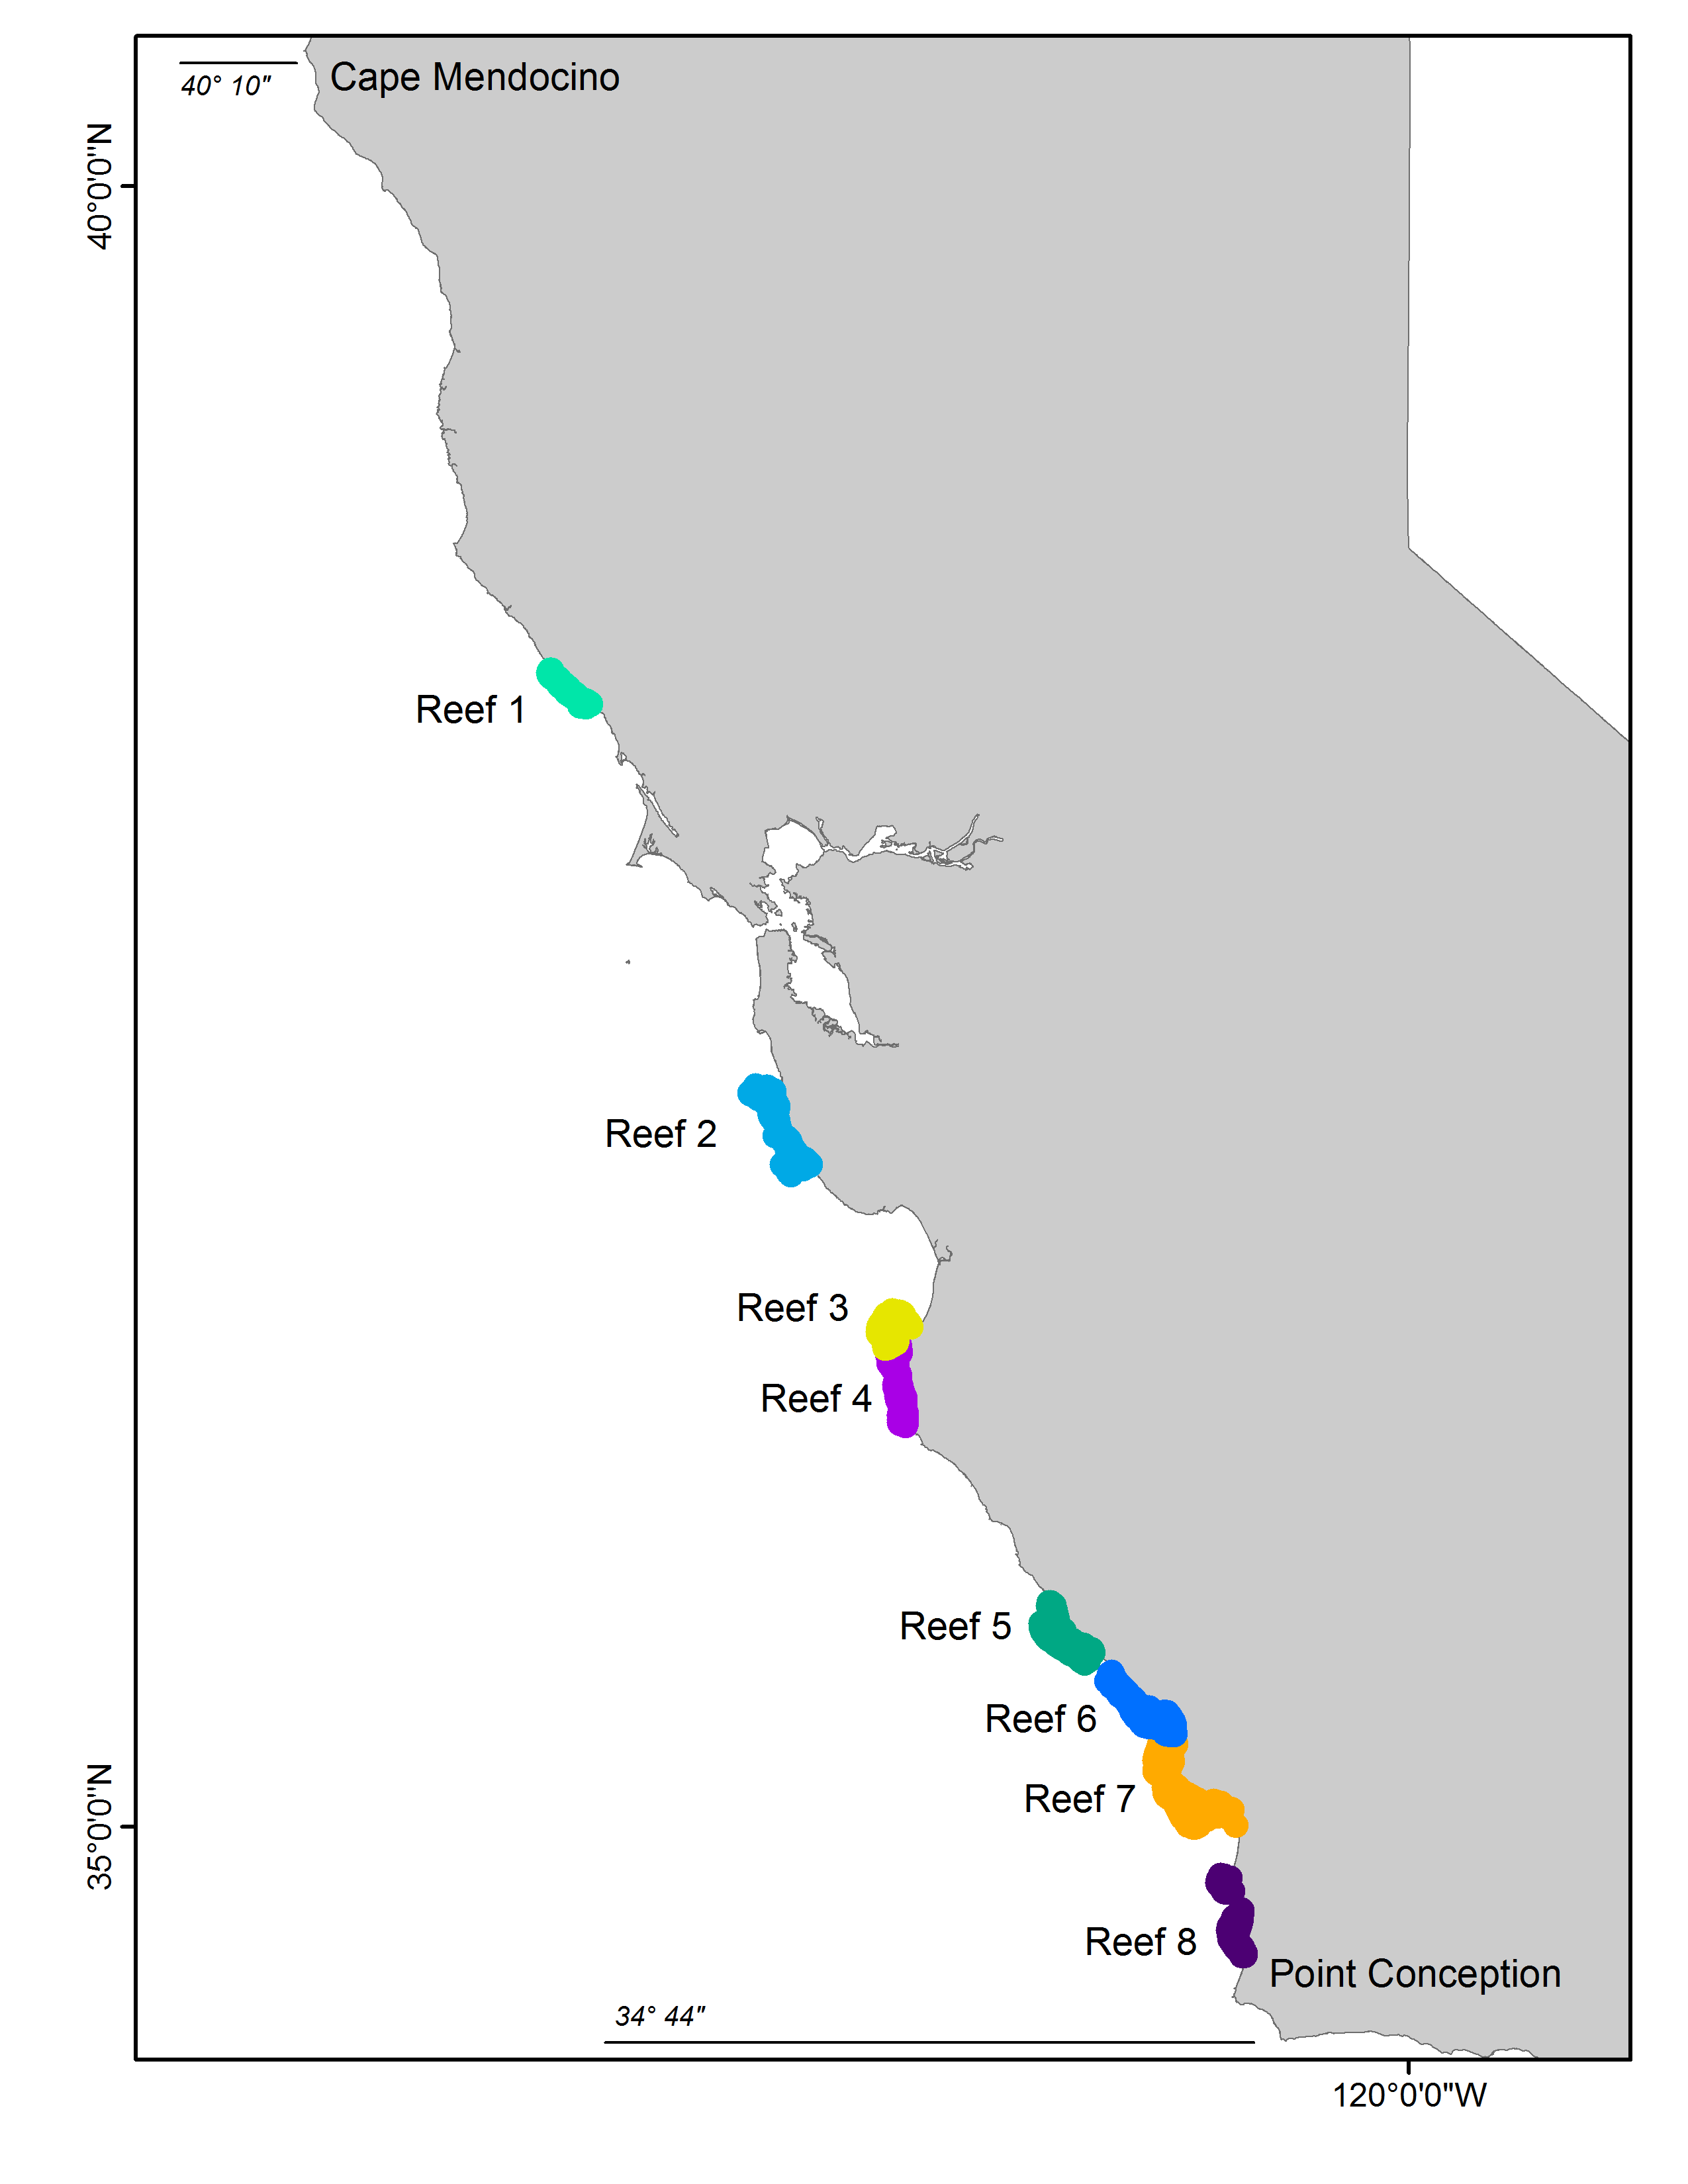
\includegraphics{Figures/DebWV_sites.png}
\caption{Map of the reefs used in the Deb Wilson-Vandenbery CPFV onboard
observer survey index of abundance. \label{fig:DebWV_sites}}
\end{figure}

\begin{figure}
\centering
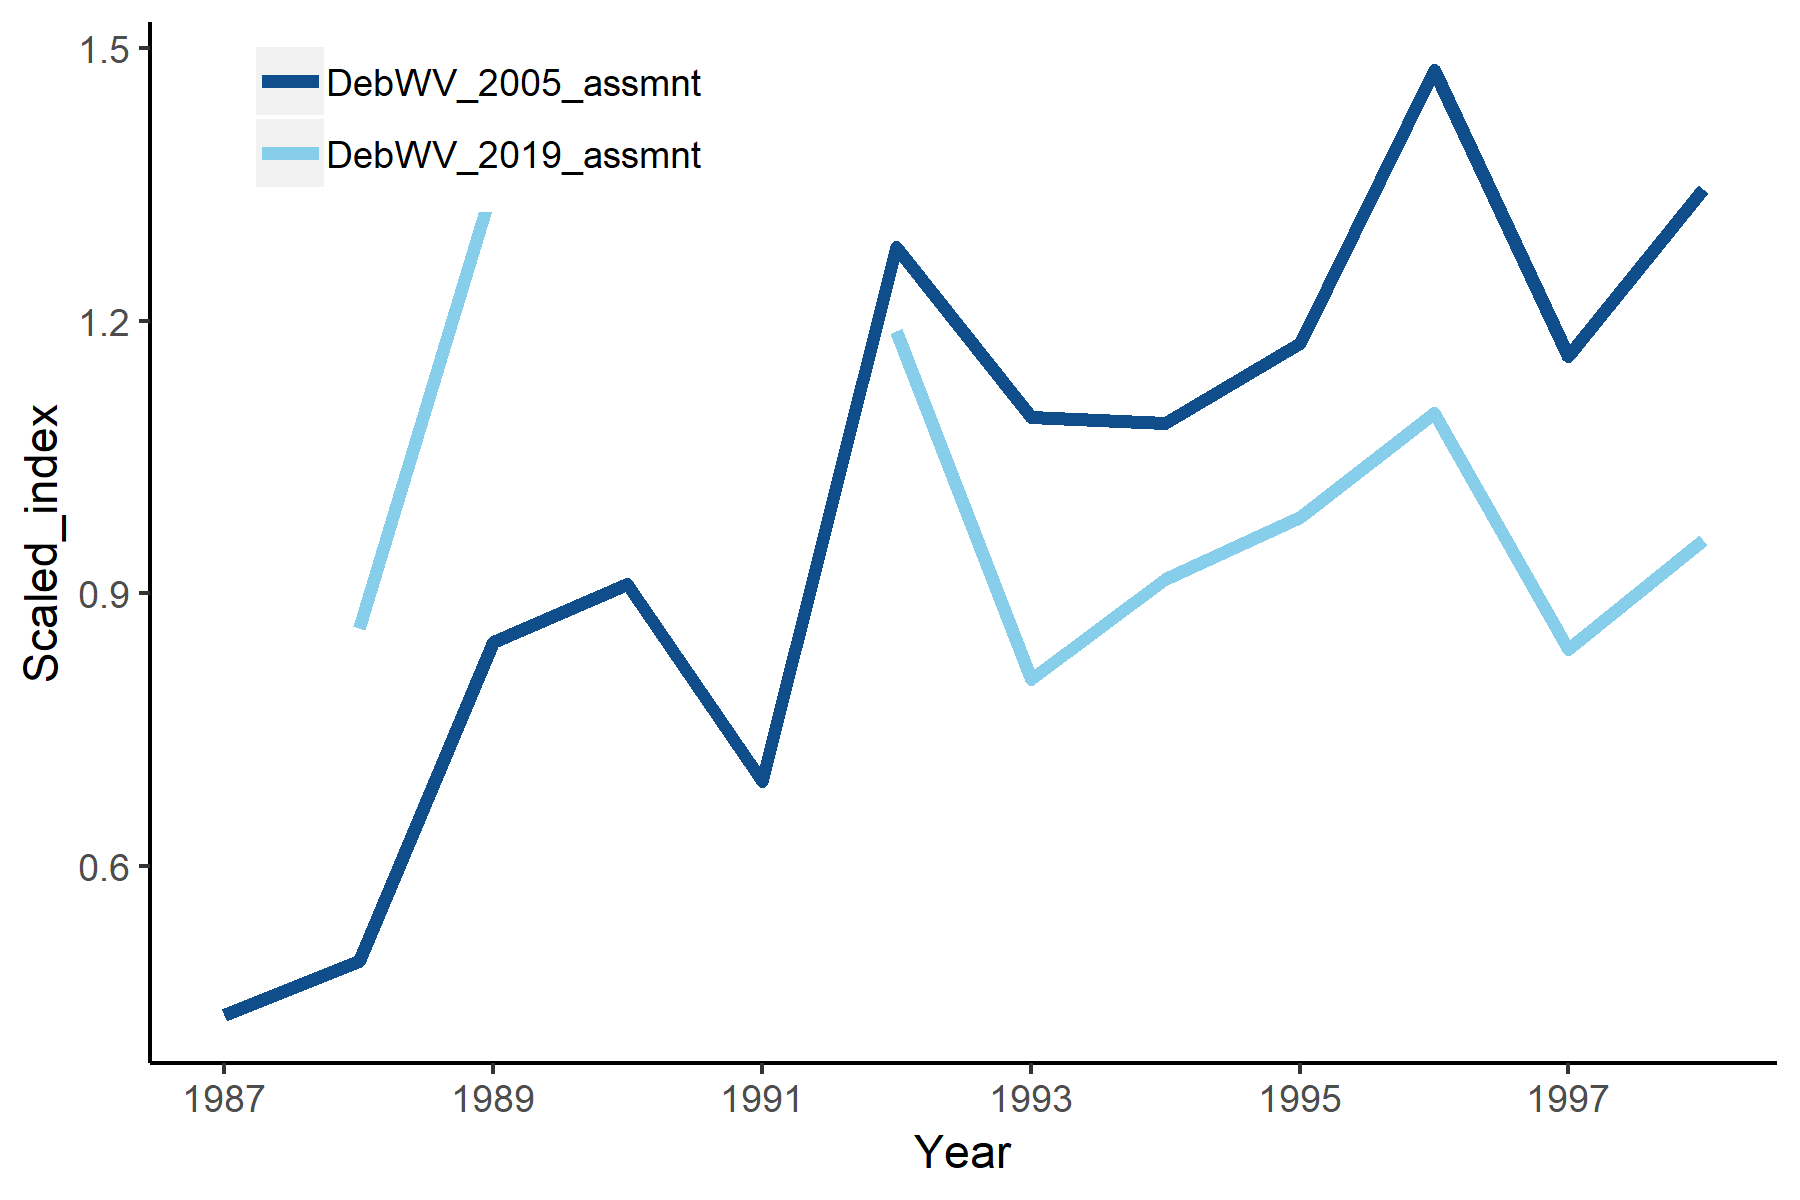
\includegraphics{Figures/DebWV_index_compare.png}
\caption{Comparison of the index developed for the Deb Wilson-Vandenbery
CPFV onboard observer survey from the 2005 assessment and forthe 2019
assessment. \label{fig:DebWV_index_compare}}
\end{figure}

\FloatBarrier

\begin{figure}
\centering
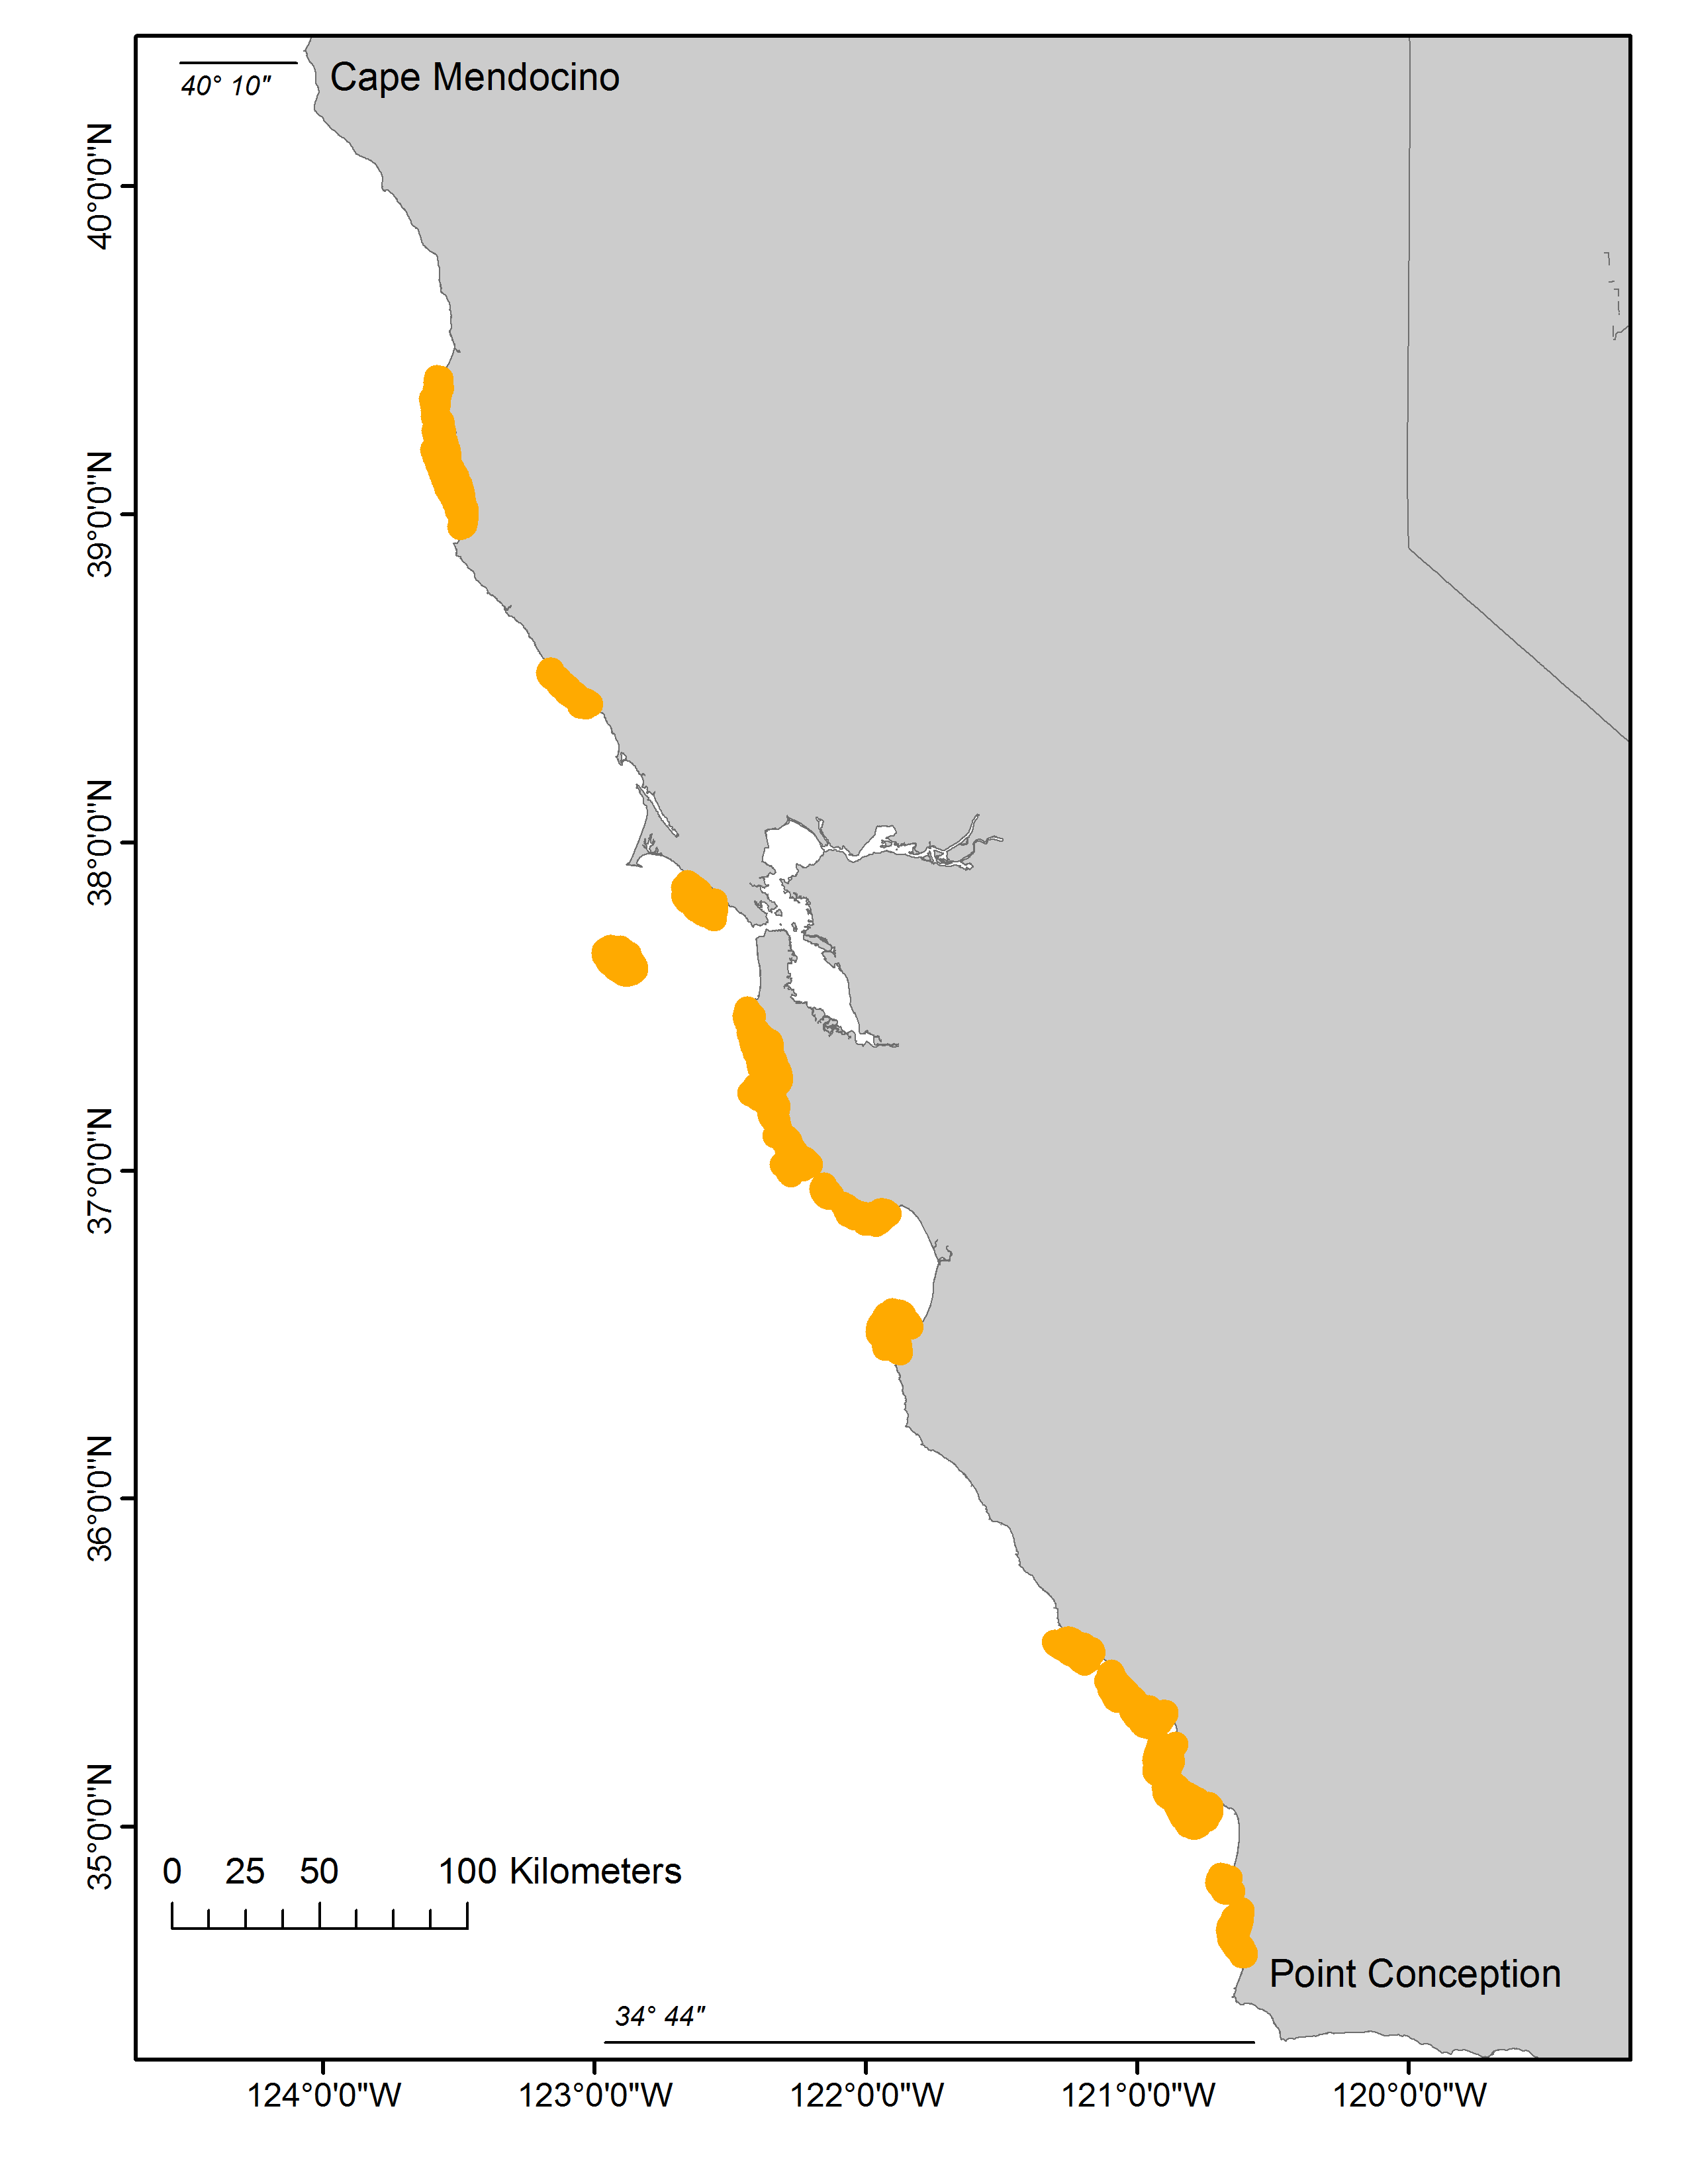
\includegraphics{Figures/Onboard_observer_north_sites.png}
\caption{Map of the reefs selected for the final index for the onboard
observer surveys (CDFW and Cal Poly) north of Point Conception
\label{fig:Onboard_observer_north_sites}}
\end{figure}

\FloatBarrier

\begin{figure}
\centering
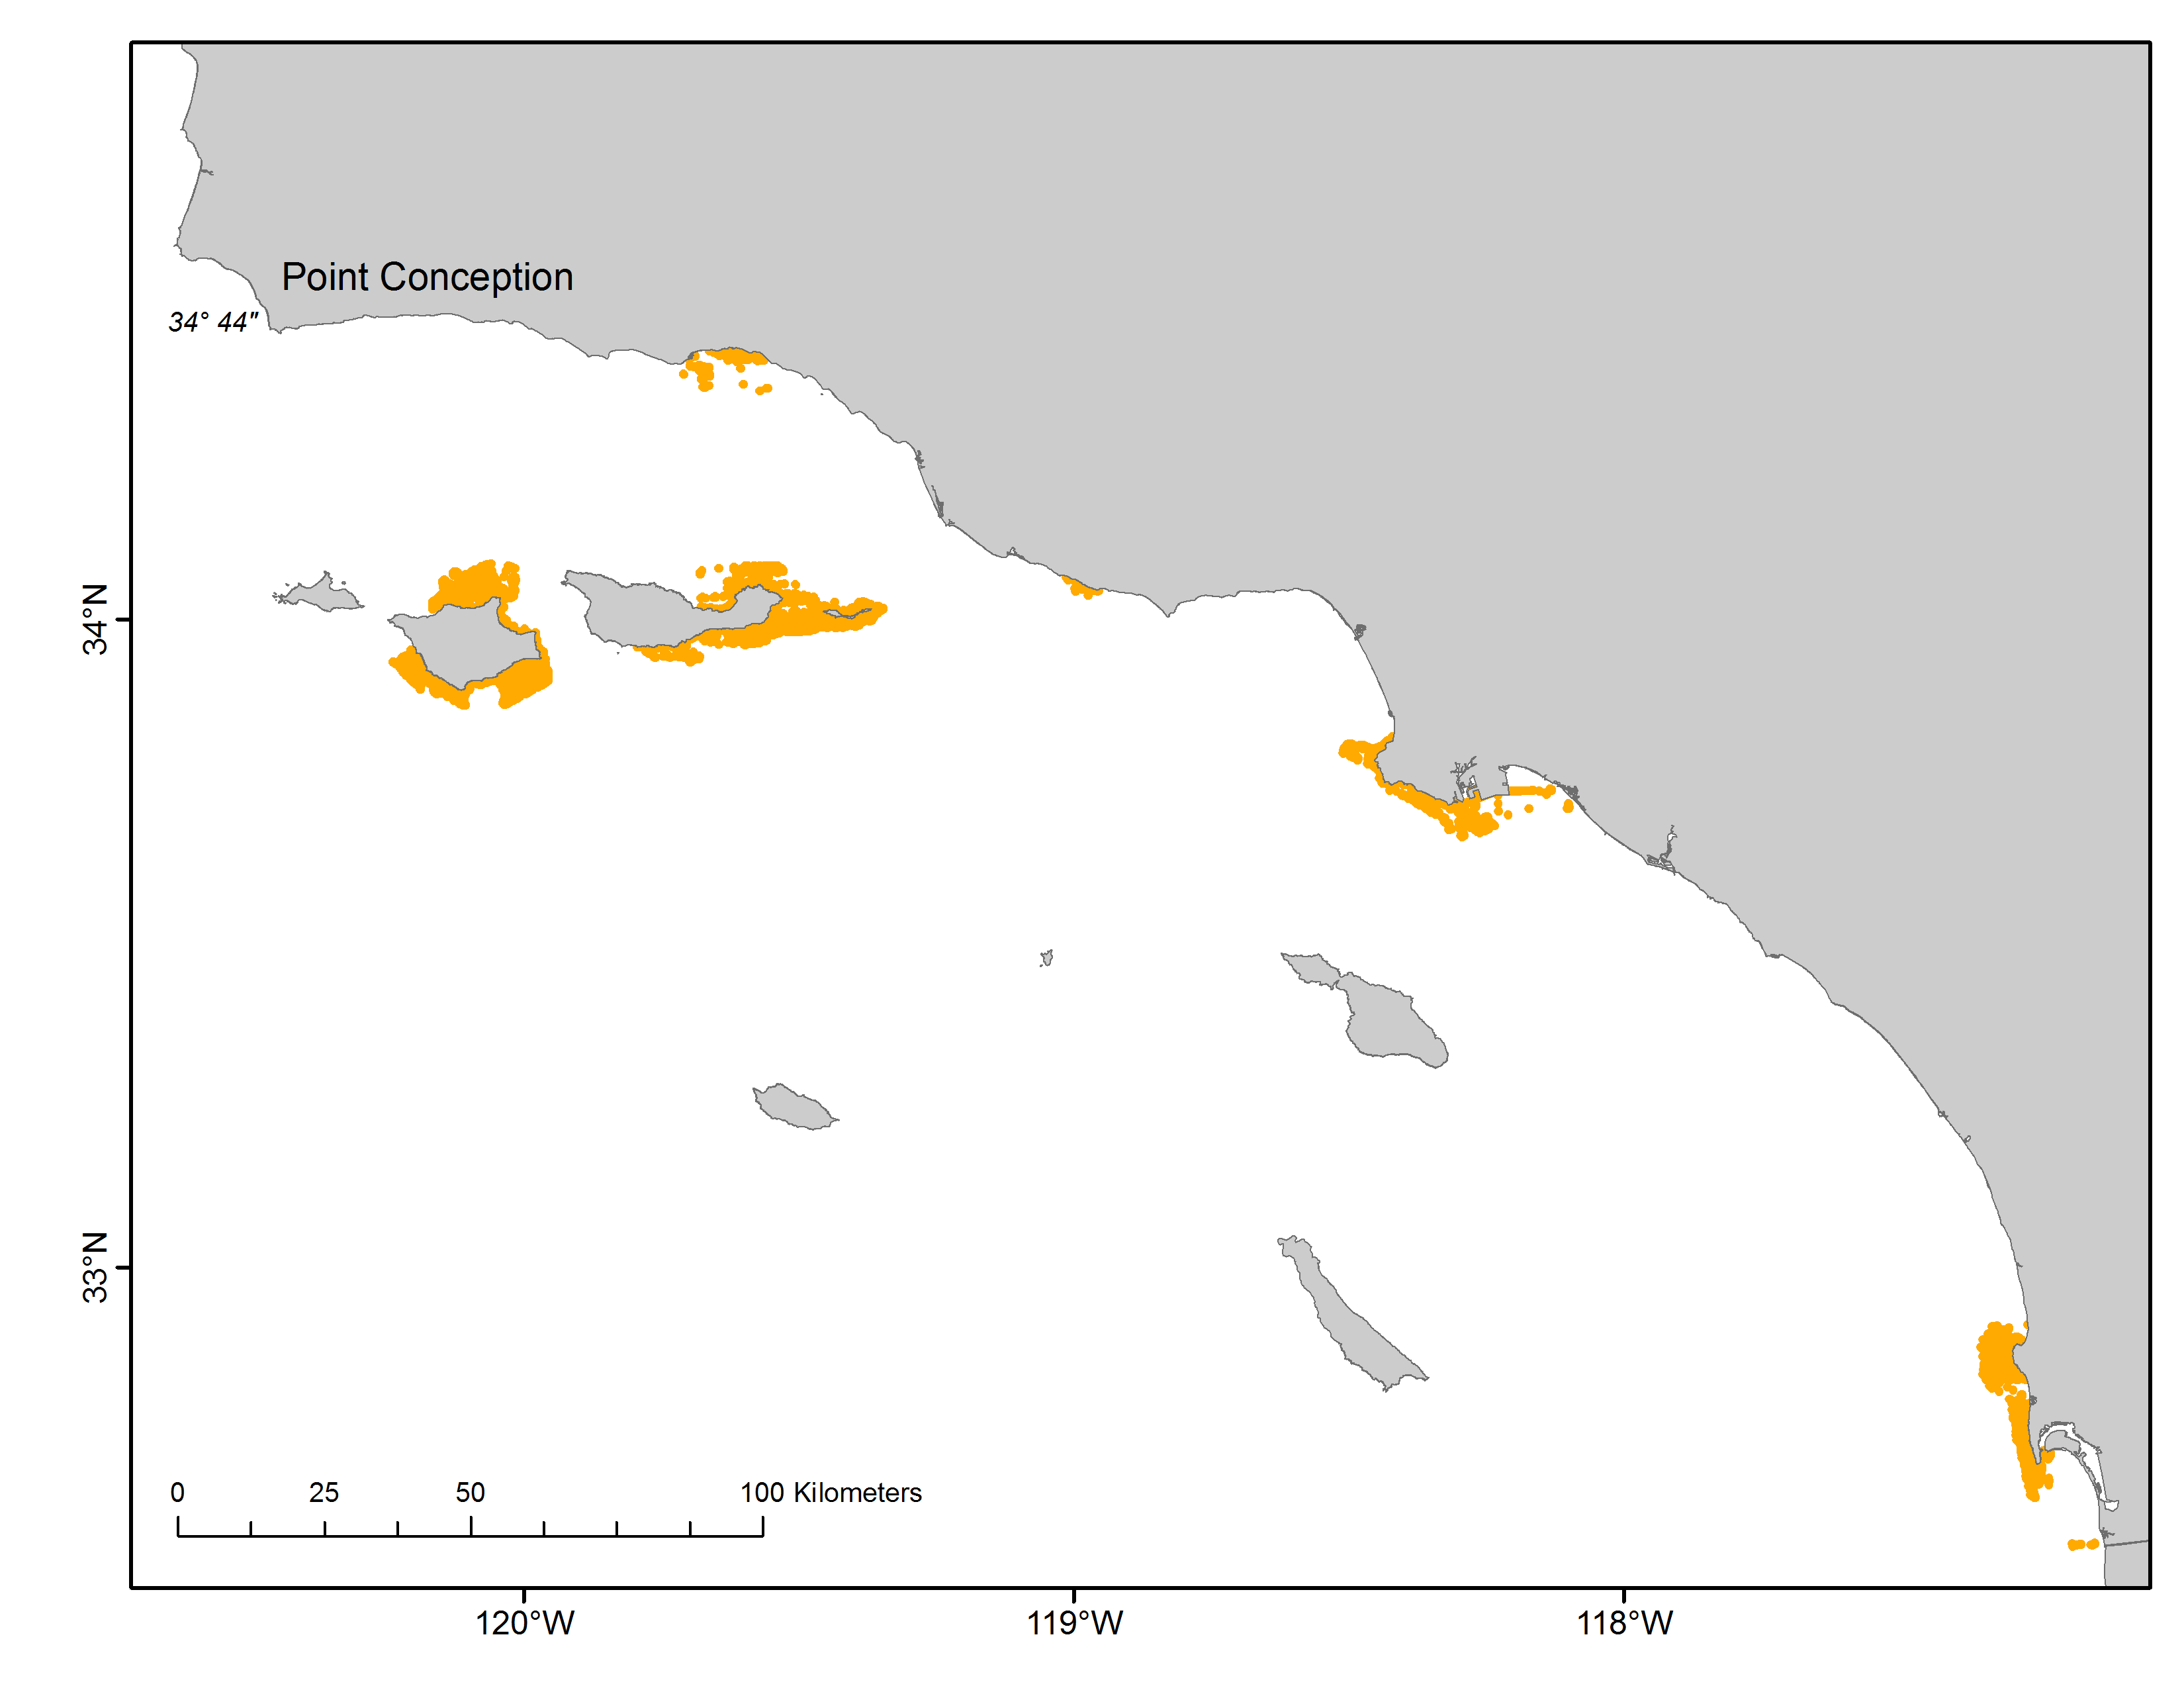
\includegraphics{Figures/Onboard_observer_south_sites.png}
\caption{Map of the reefs selected for the final index for the CDFW
onboard observer survey south of Point Conception
\label{fig:Onboard_observer_south_sites}}
\end{figure}

\FloatBarrier 

\begin{figure}
\centering
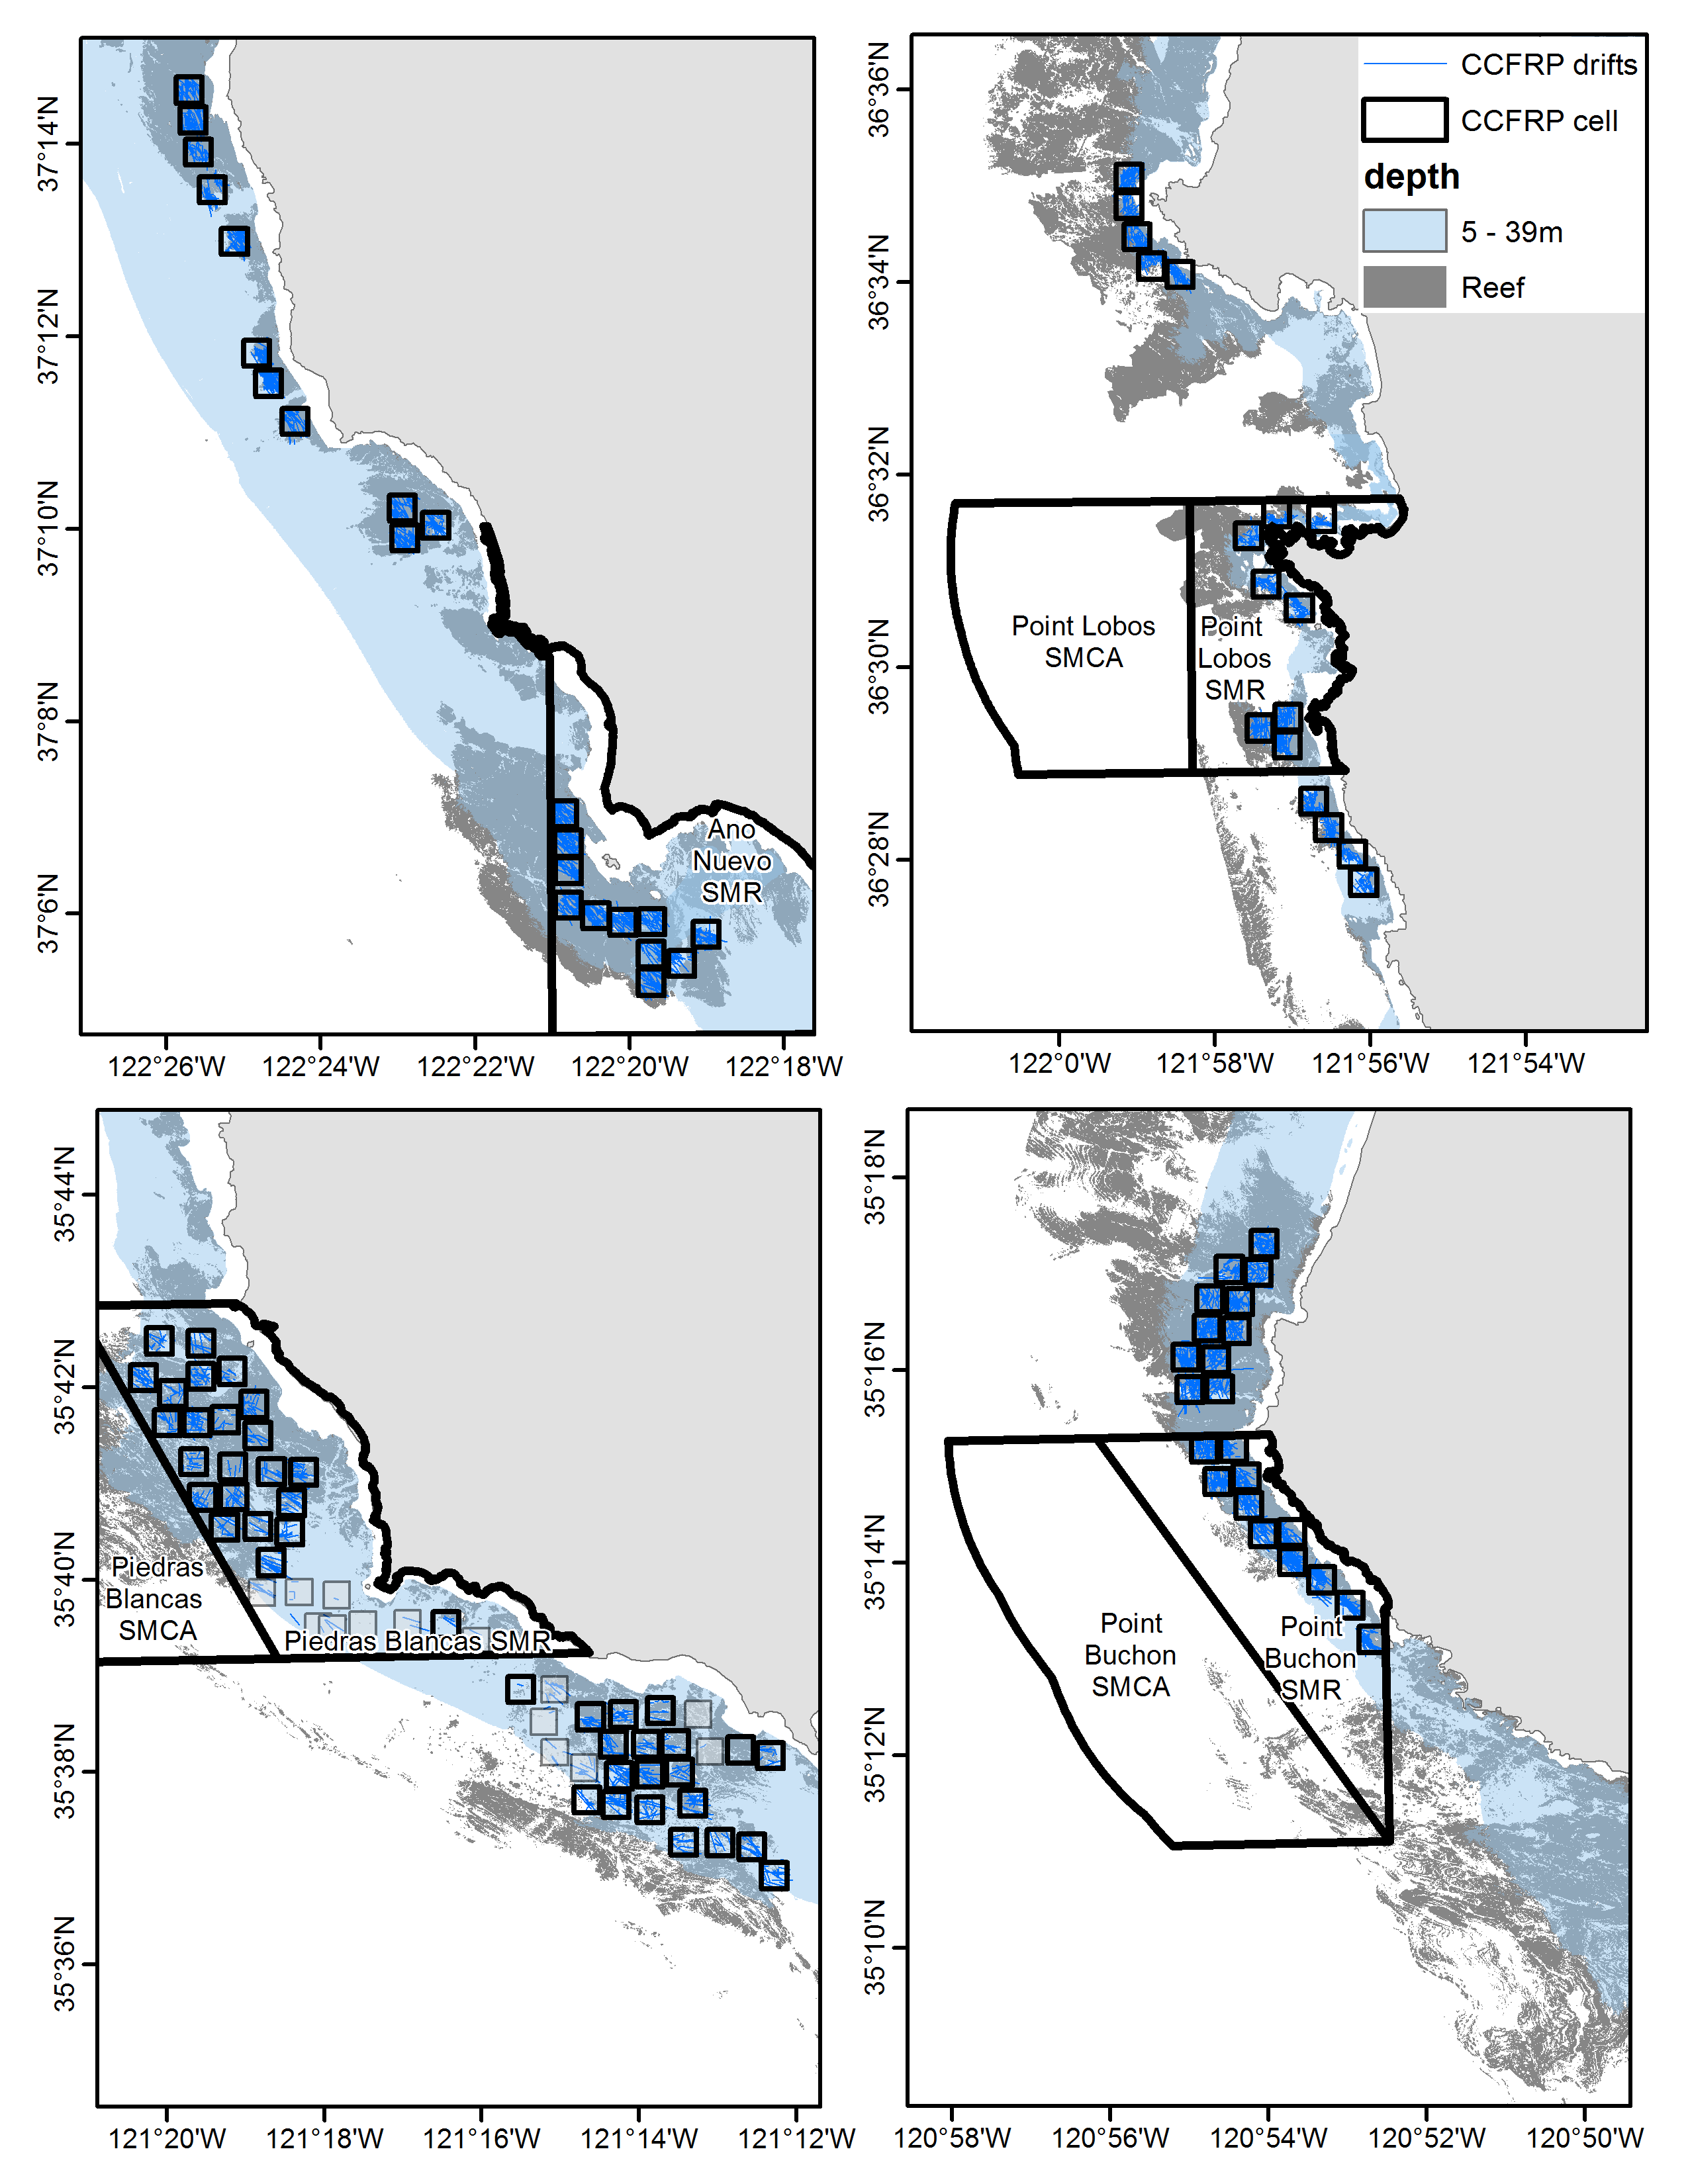
\includegraphics{Figures/CCFRP_sites.png}
\caption{Map of the four MPAs sample consistently through time for the
CCFRP fishery-independent survey. \label{fig:CCFRP_sites}}
\end{figure}

\FloatBarrier

\begin{figure}
\centering
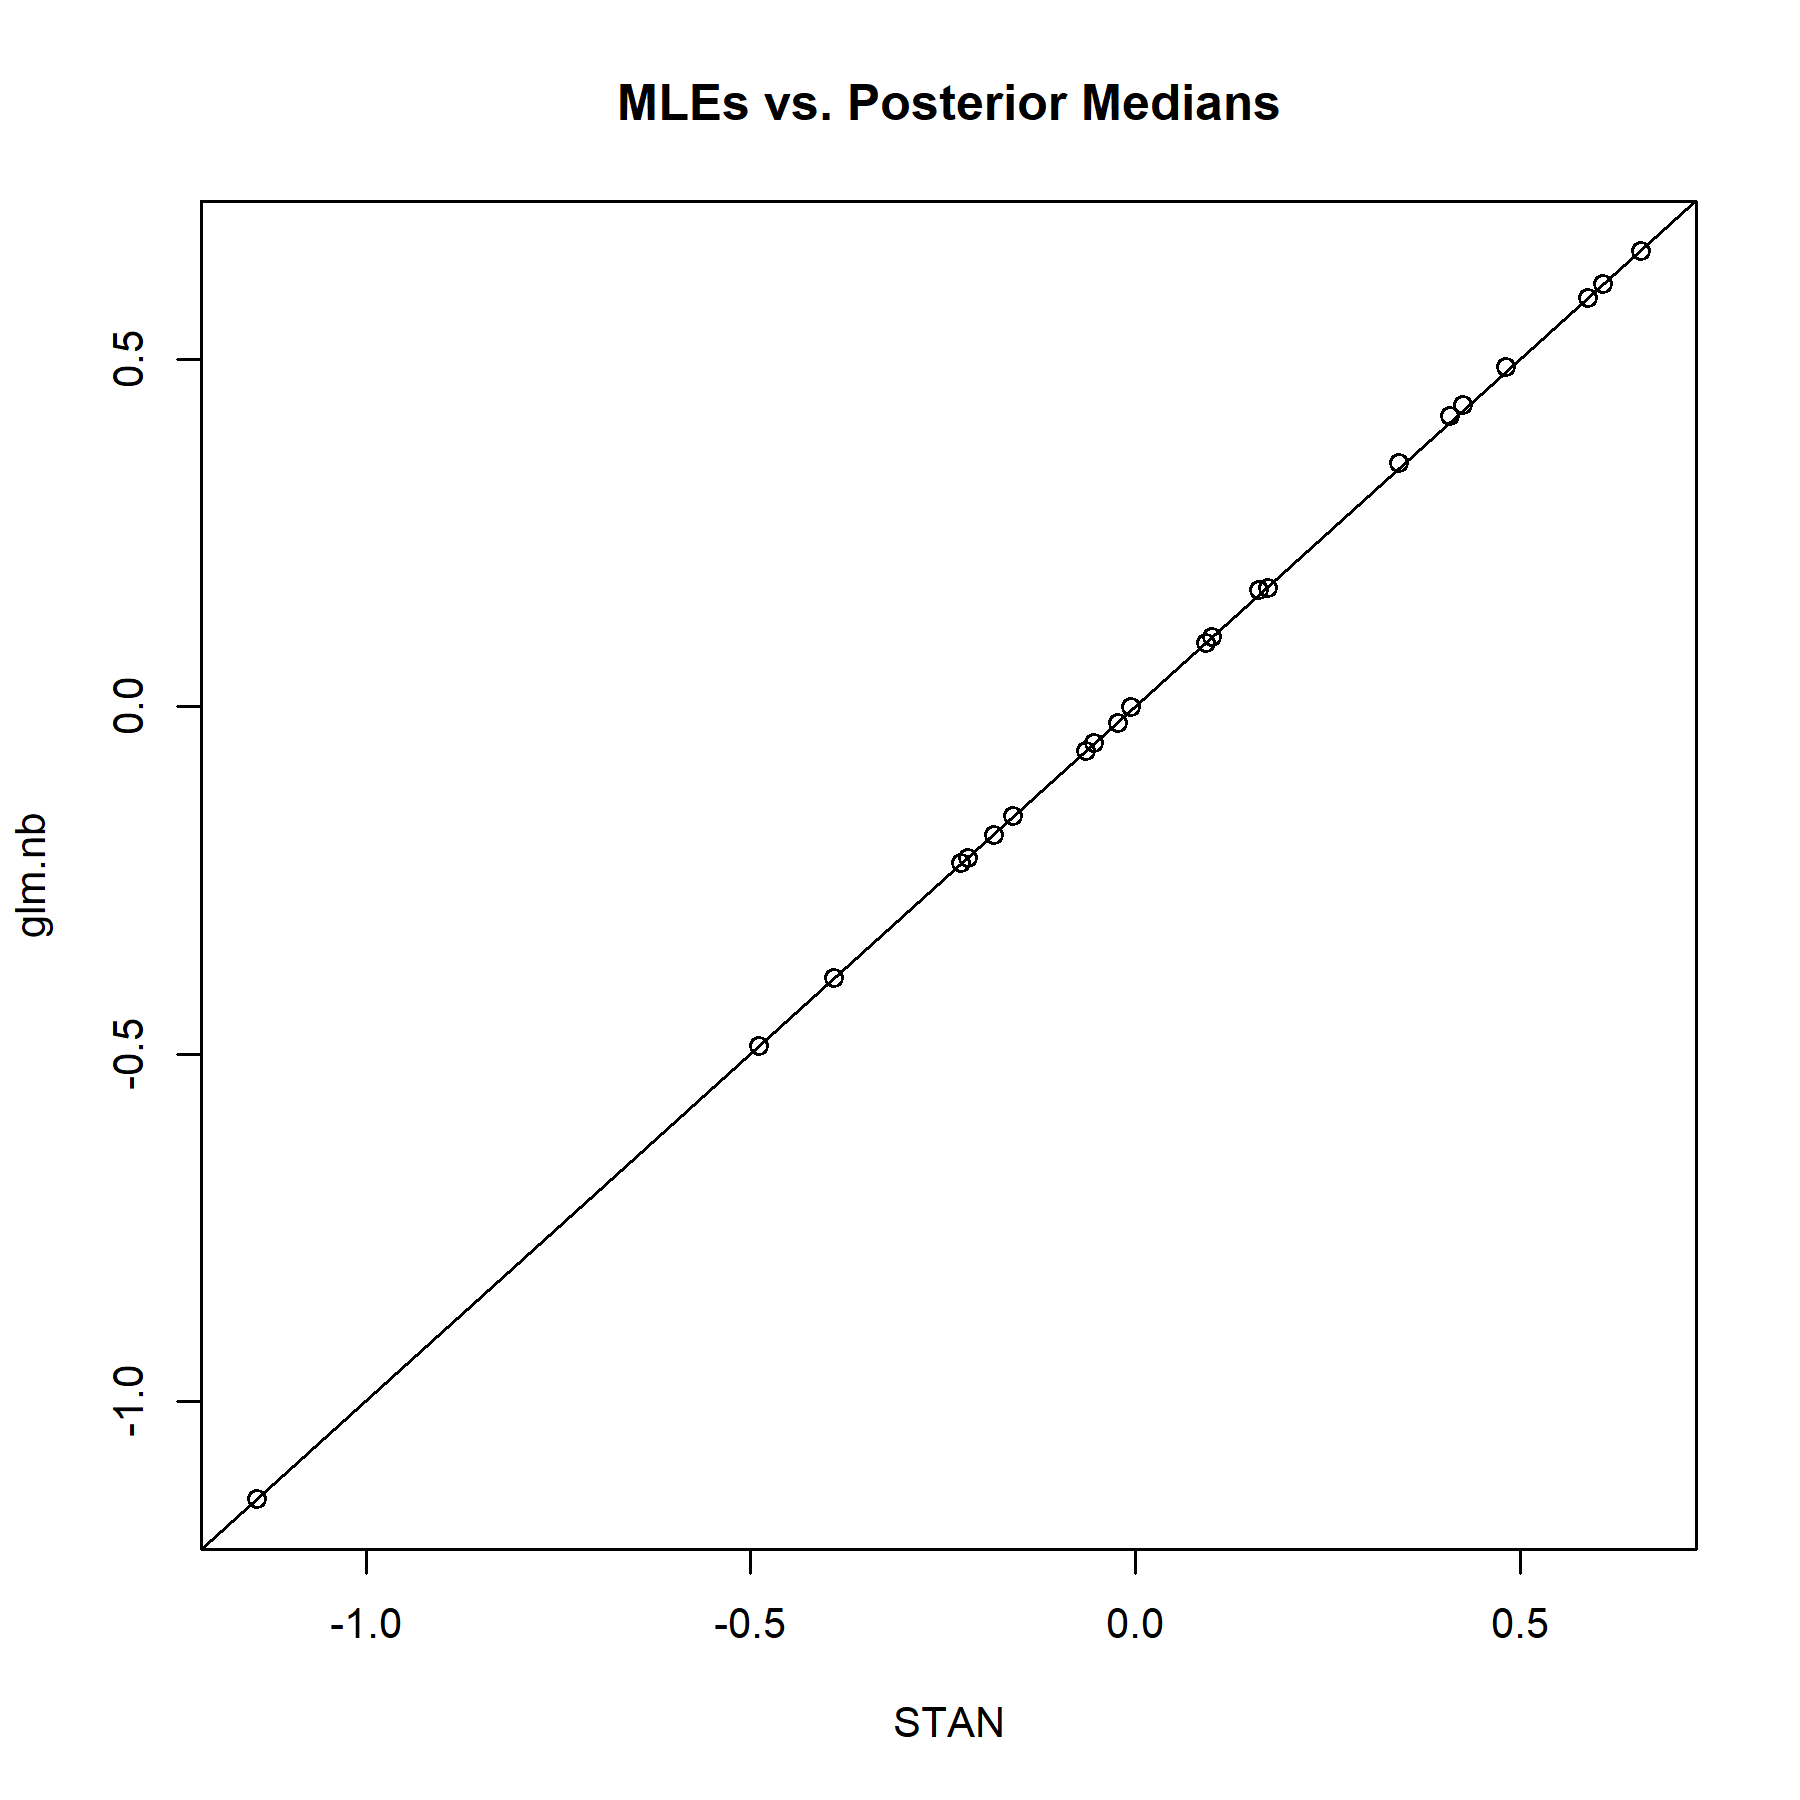
\includegraphics{Figures/Fleet9_MLE_stan.png}
\caption{Comparison of negative bionimial predictions (CPUE) to observed
means in each stratum (year) for the CCFRP index. The 1:1 plot is for
reference. \label{fig:Fleet9_MLE_stan}}
\end{figure}

\FloatBarrier

\begin{figure}
\centering
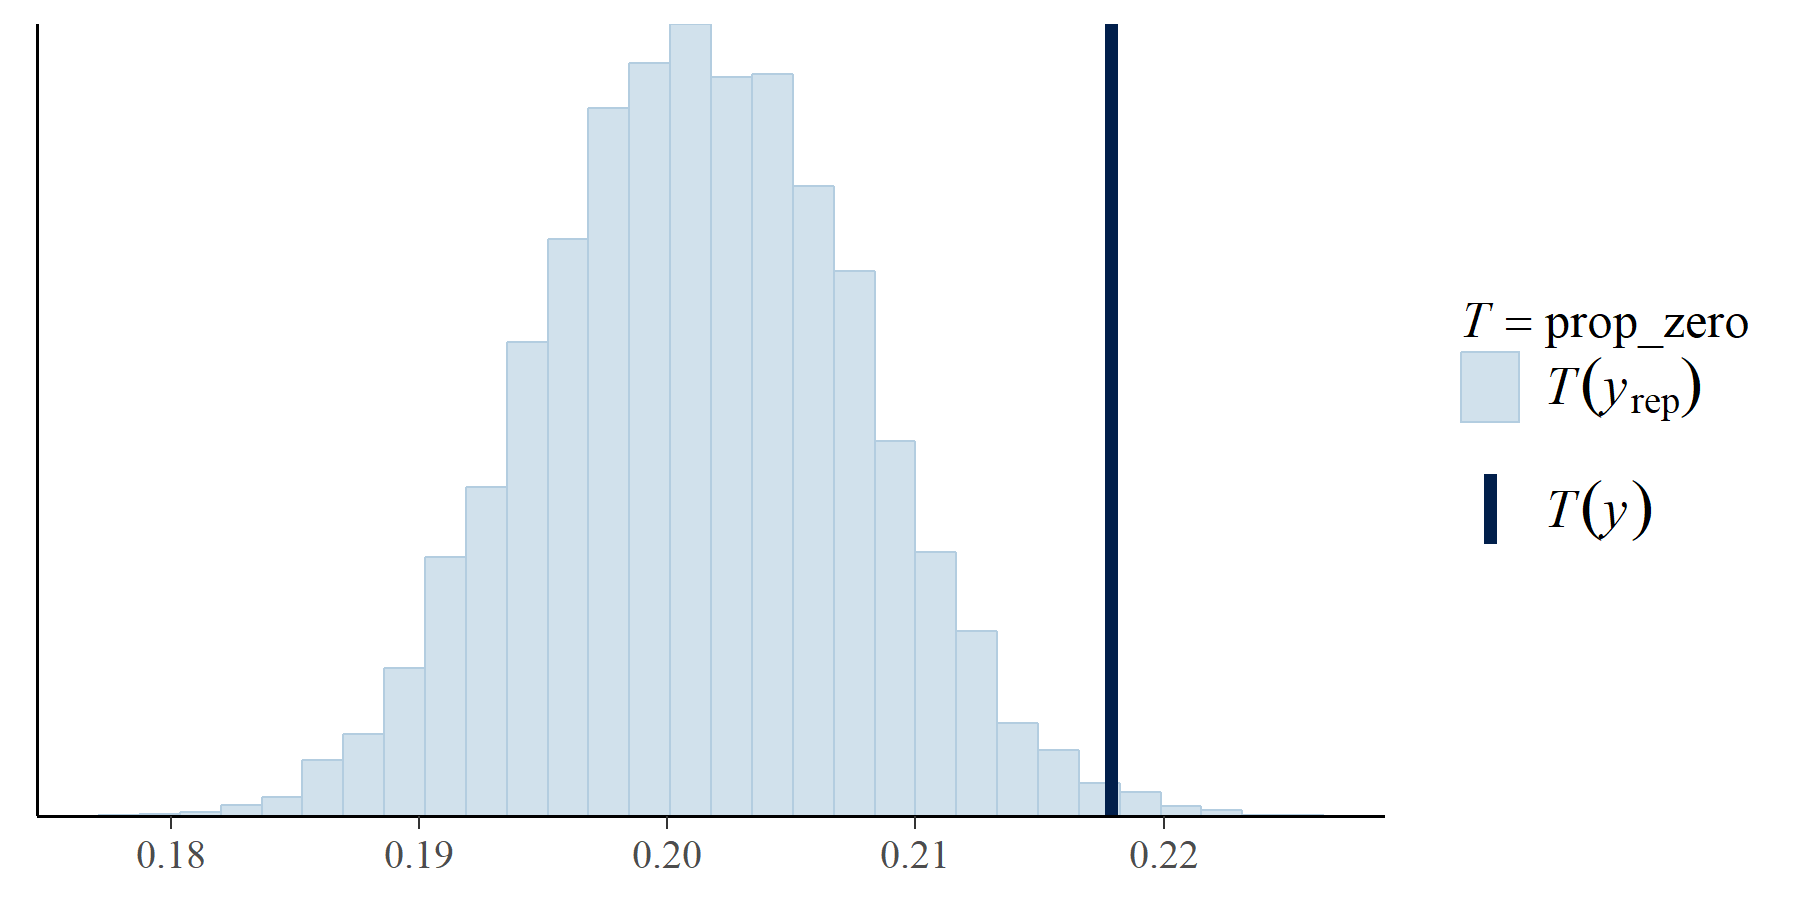
\includegraphics{Figures/Fleet9_prop_zero_STAN.png}
\caption{Posterior predictive distribution of the proportion of zero
observations in replicate data sets generated by the negative binomial
model for the CCFRP index. \label{fig:Fleet9_prop_zero_STAN}}
\end{figure}

\FloatBarrier

\begin{figure}
\centering
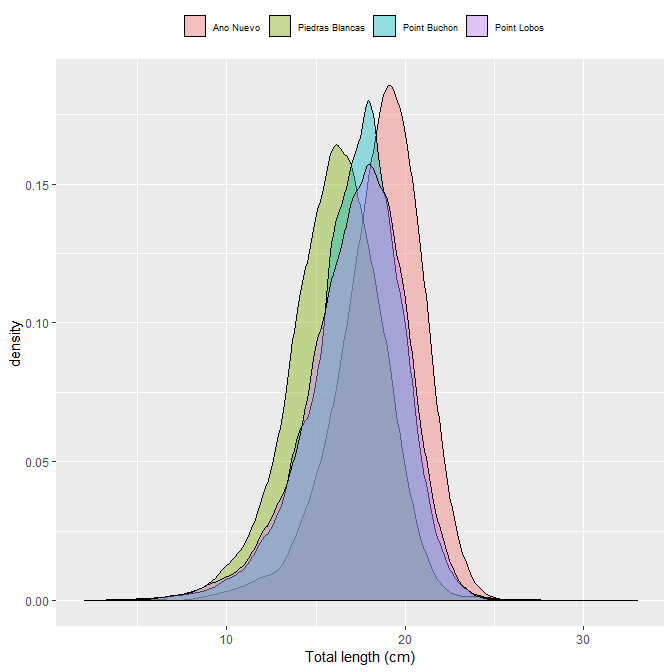
\includegraphics{Figures/CCFRP_lengths_by_site.png}
\caption{Length distributions of GBYR for the four MPAs sampled by the
CCFRP survey used in this assessment. \label{CCFRP_lengths_by_site}}
\end{figure}

\begin{figure}
\centering
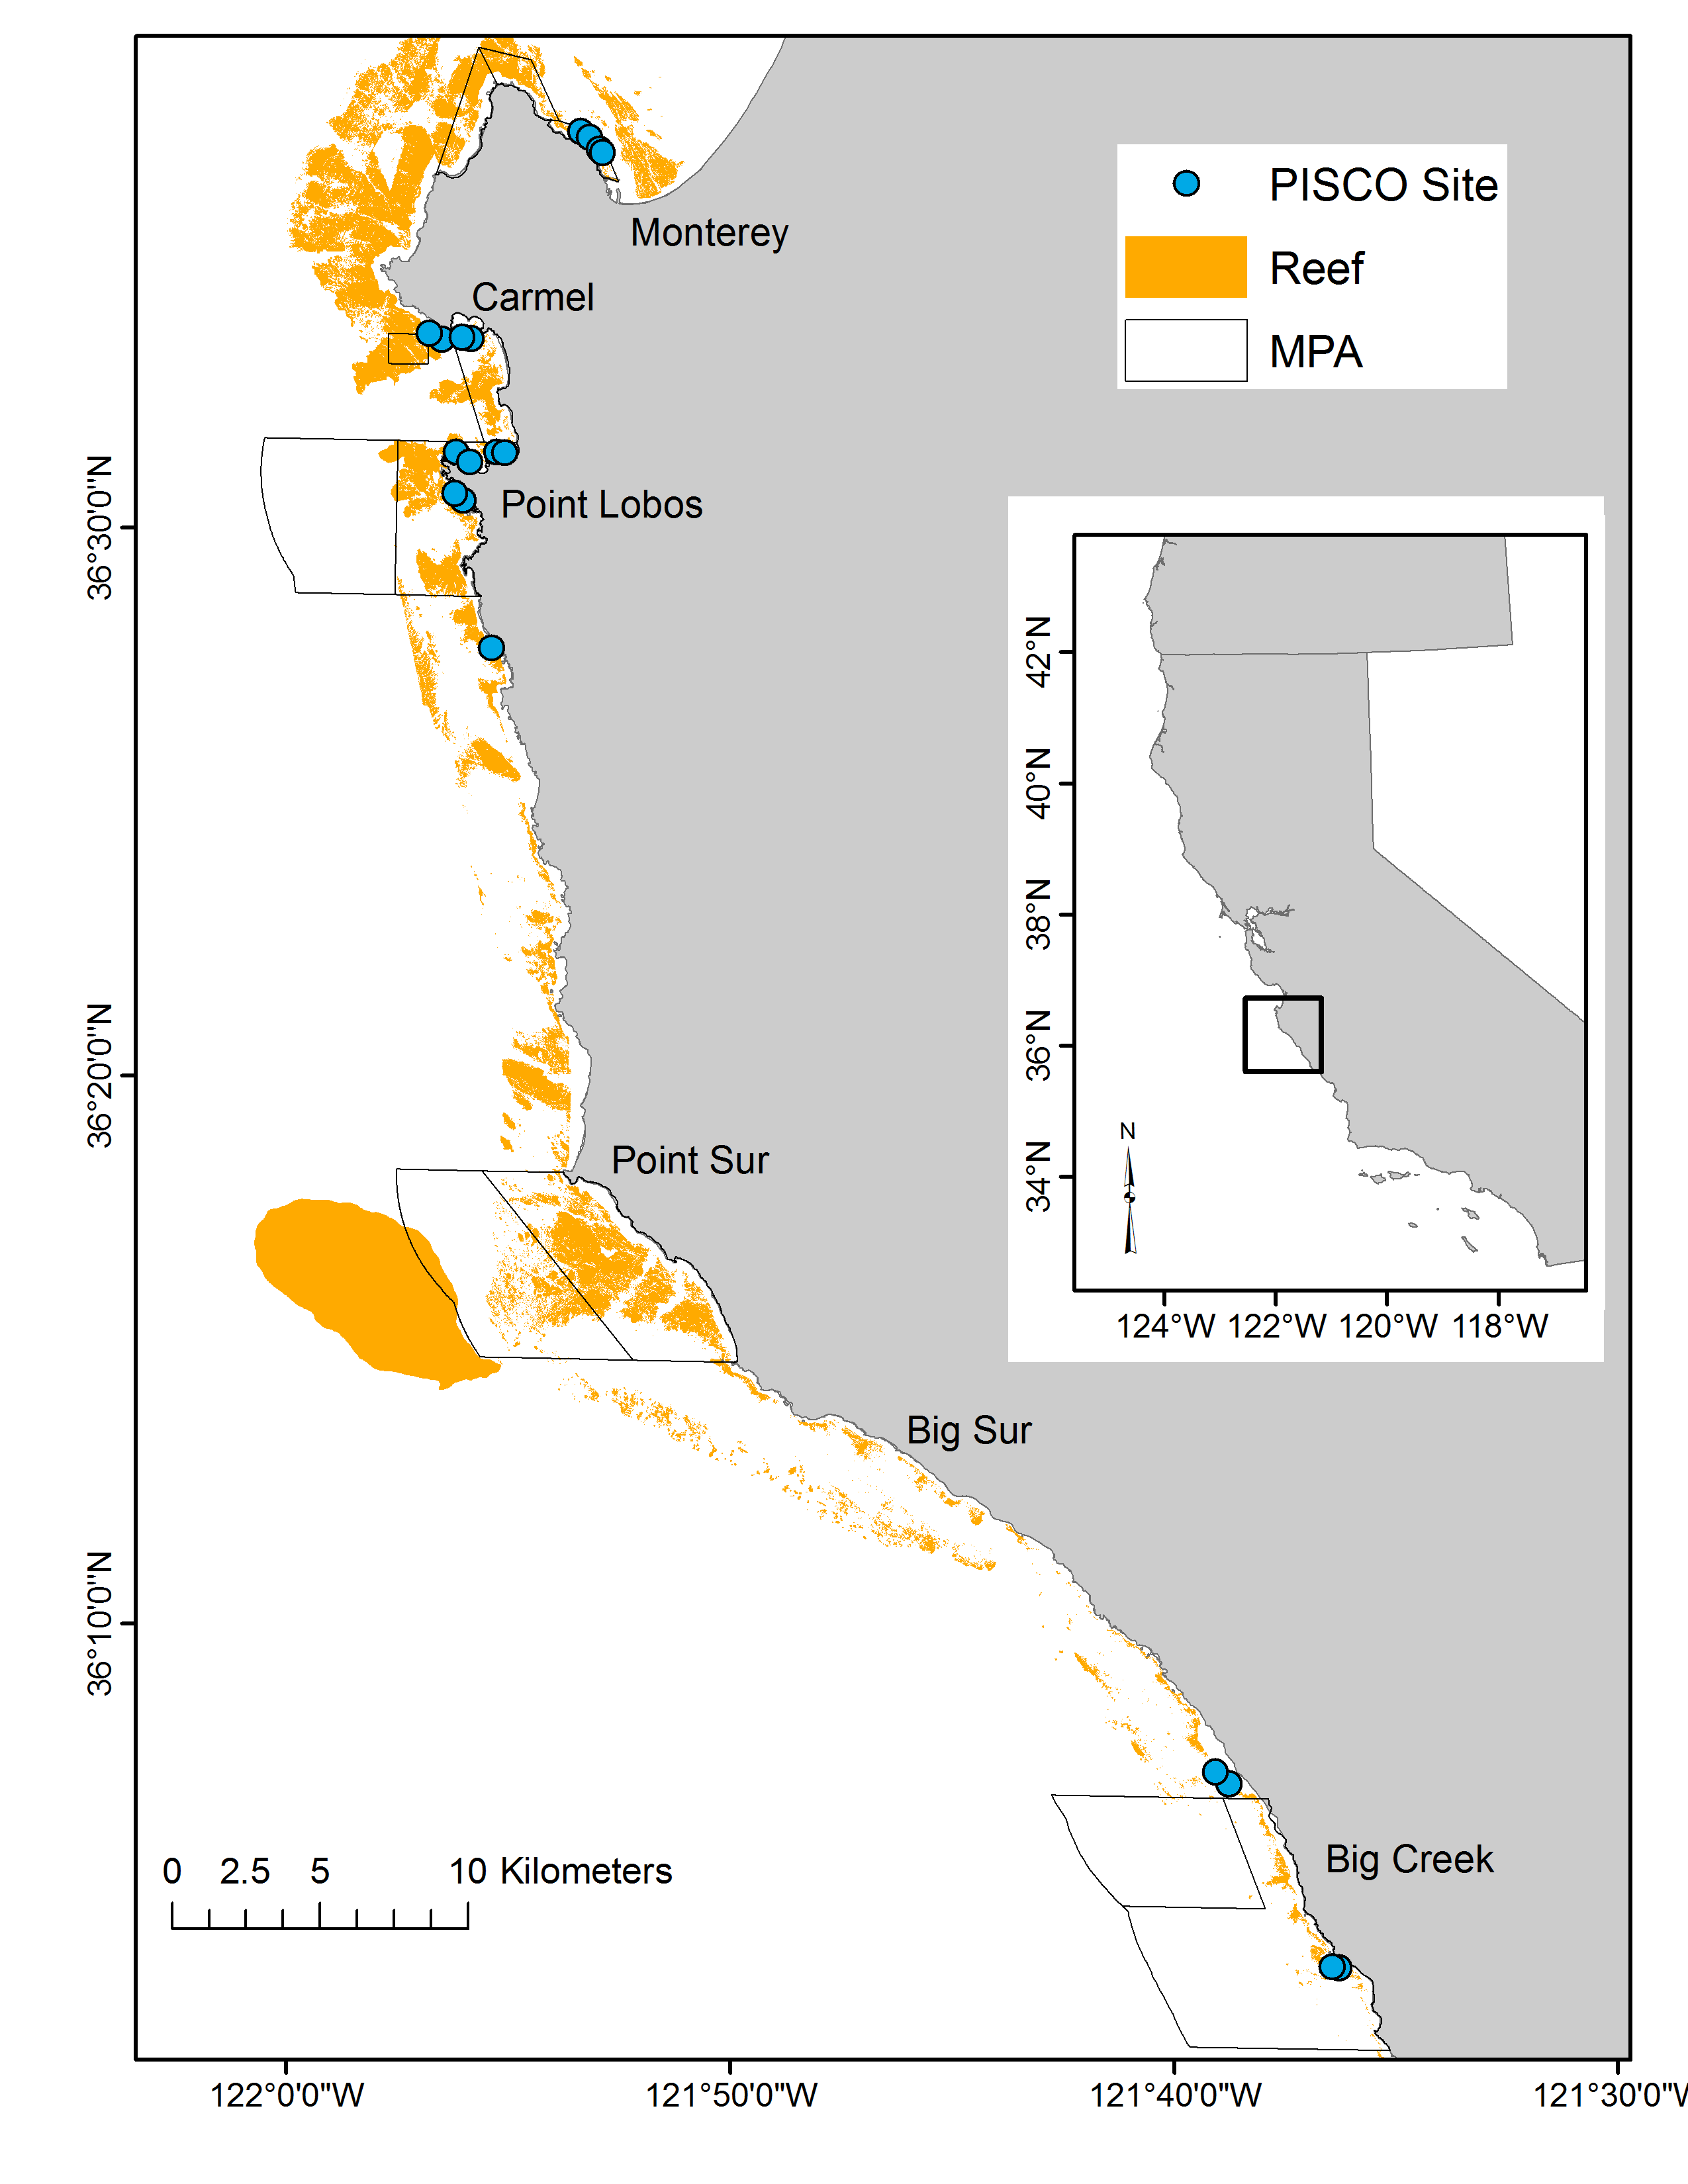
\includegraphics{Figures/PISCO_sites.png}
\caption{Map of the sites sampled consistently through time for the
PISCO kelp forest fish survey. \label{fig:PISCO_sites}}
\end{figure}

\FloatBarrier

\begin{figure}
\centering
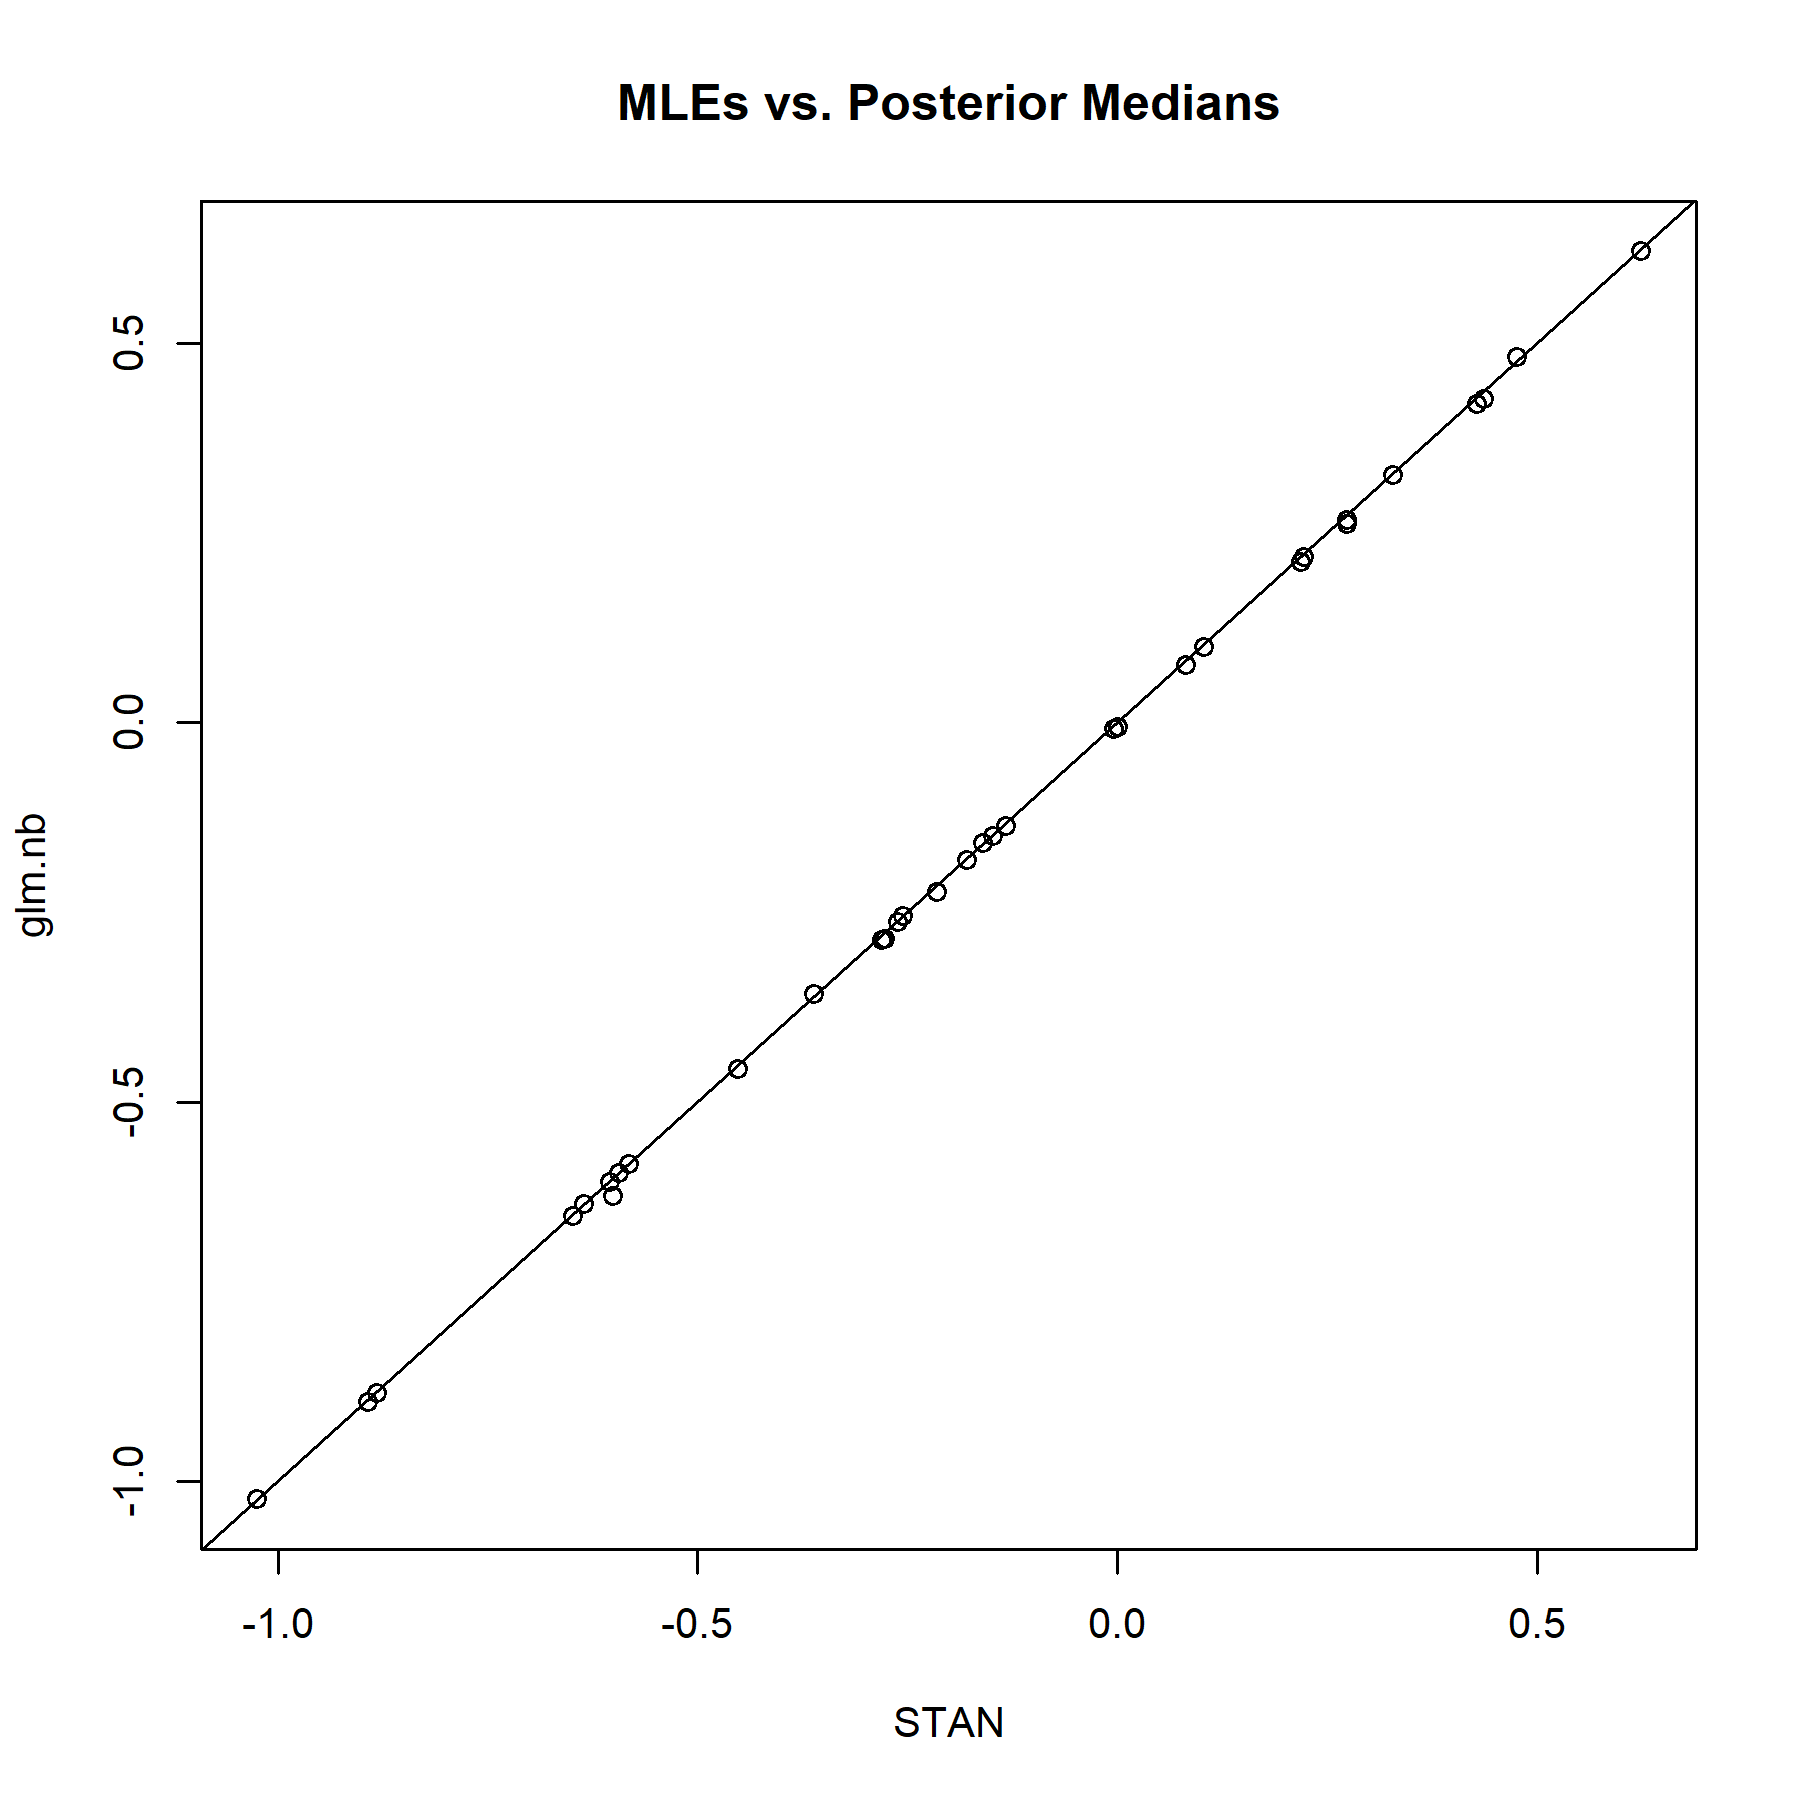
\includegraphics{Figures/Fleet8_MLE_stan.png}
\caption{Comparison of negative bionimial predictions (CPUE) to observed
means in each stratum (year) for the PISCO kelp forest fish survey
index. The 1:1 plot is for reference. \label{fig:Fleet8_MLE_stan}}
\end{figure}

\FloatBarrier

\begin{figure}
\centering
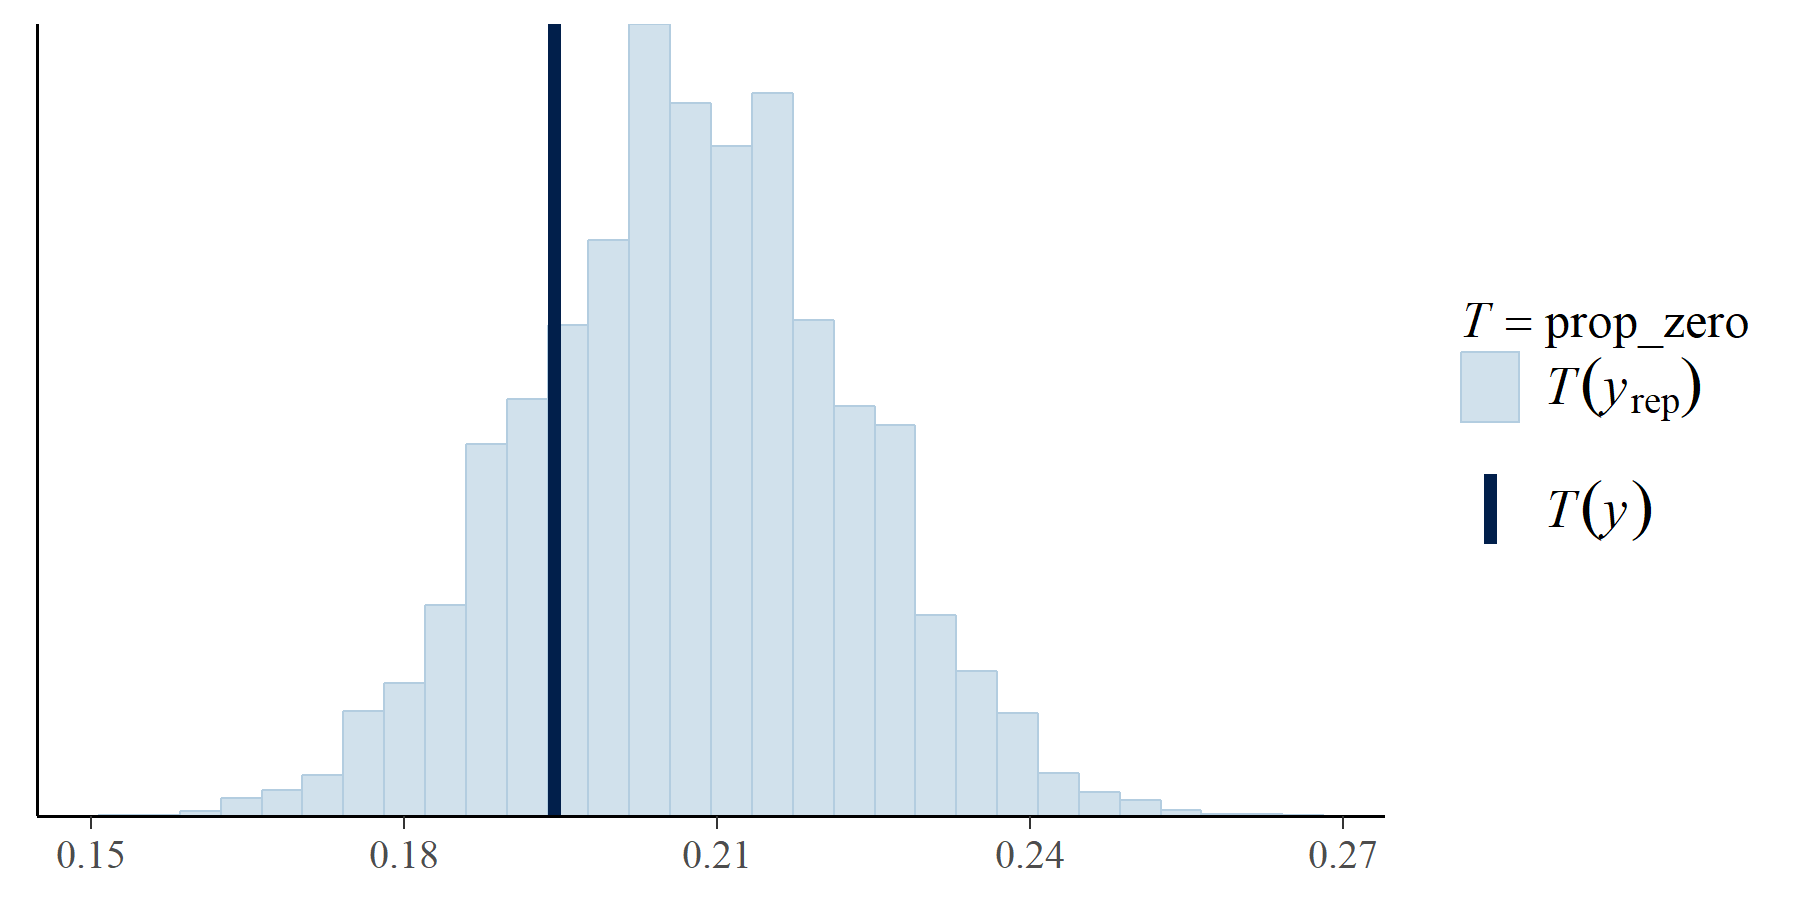
\includegraphics{Figures/Fleet8_prop_zero_STAN.png}
\caption{Posterior predictive distribution of the proportion of zero
observations in replicate data sets generated by the negative binomial
model for the PISCO kelp forest fish survey.
\label{fig:Fleet8_prop_zero_STAN}}
\end{figure}

\FloatBarrier

\begin{figure}
\centering
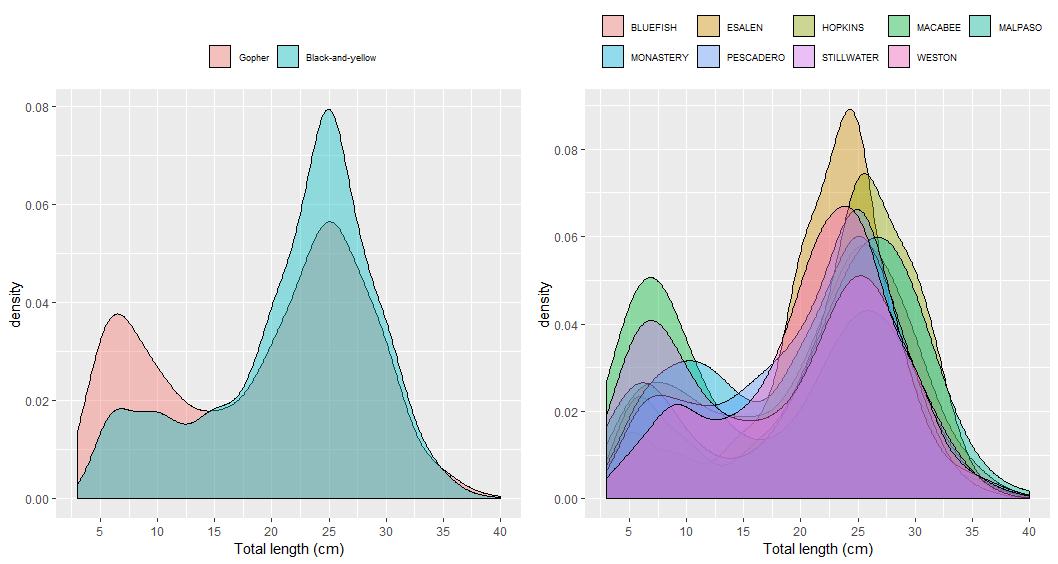
\includegraphics{Figures/PISCO_lengths.png}
\caption{Plots of the length distributions from the PISCO kelp forest
fish survey by species (left) and for compbined species by site (right)
for sites included in the final index of abundance.
\label{fig:PISCO_lengths}}
\end{figure}

\FloatBarrier

\begin{figure}
\centering
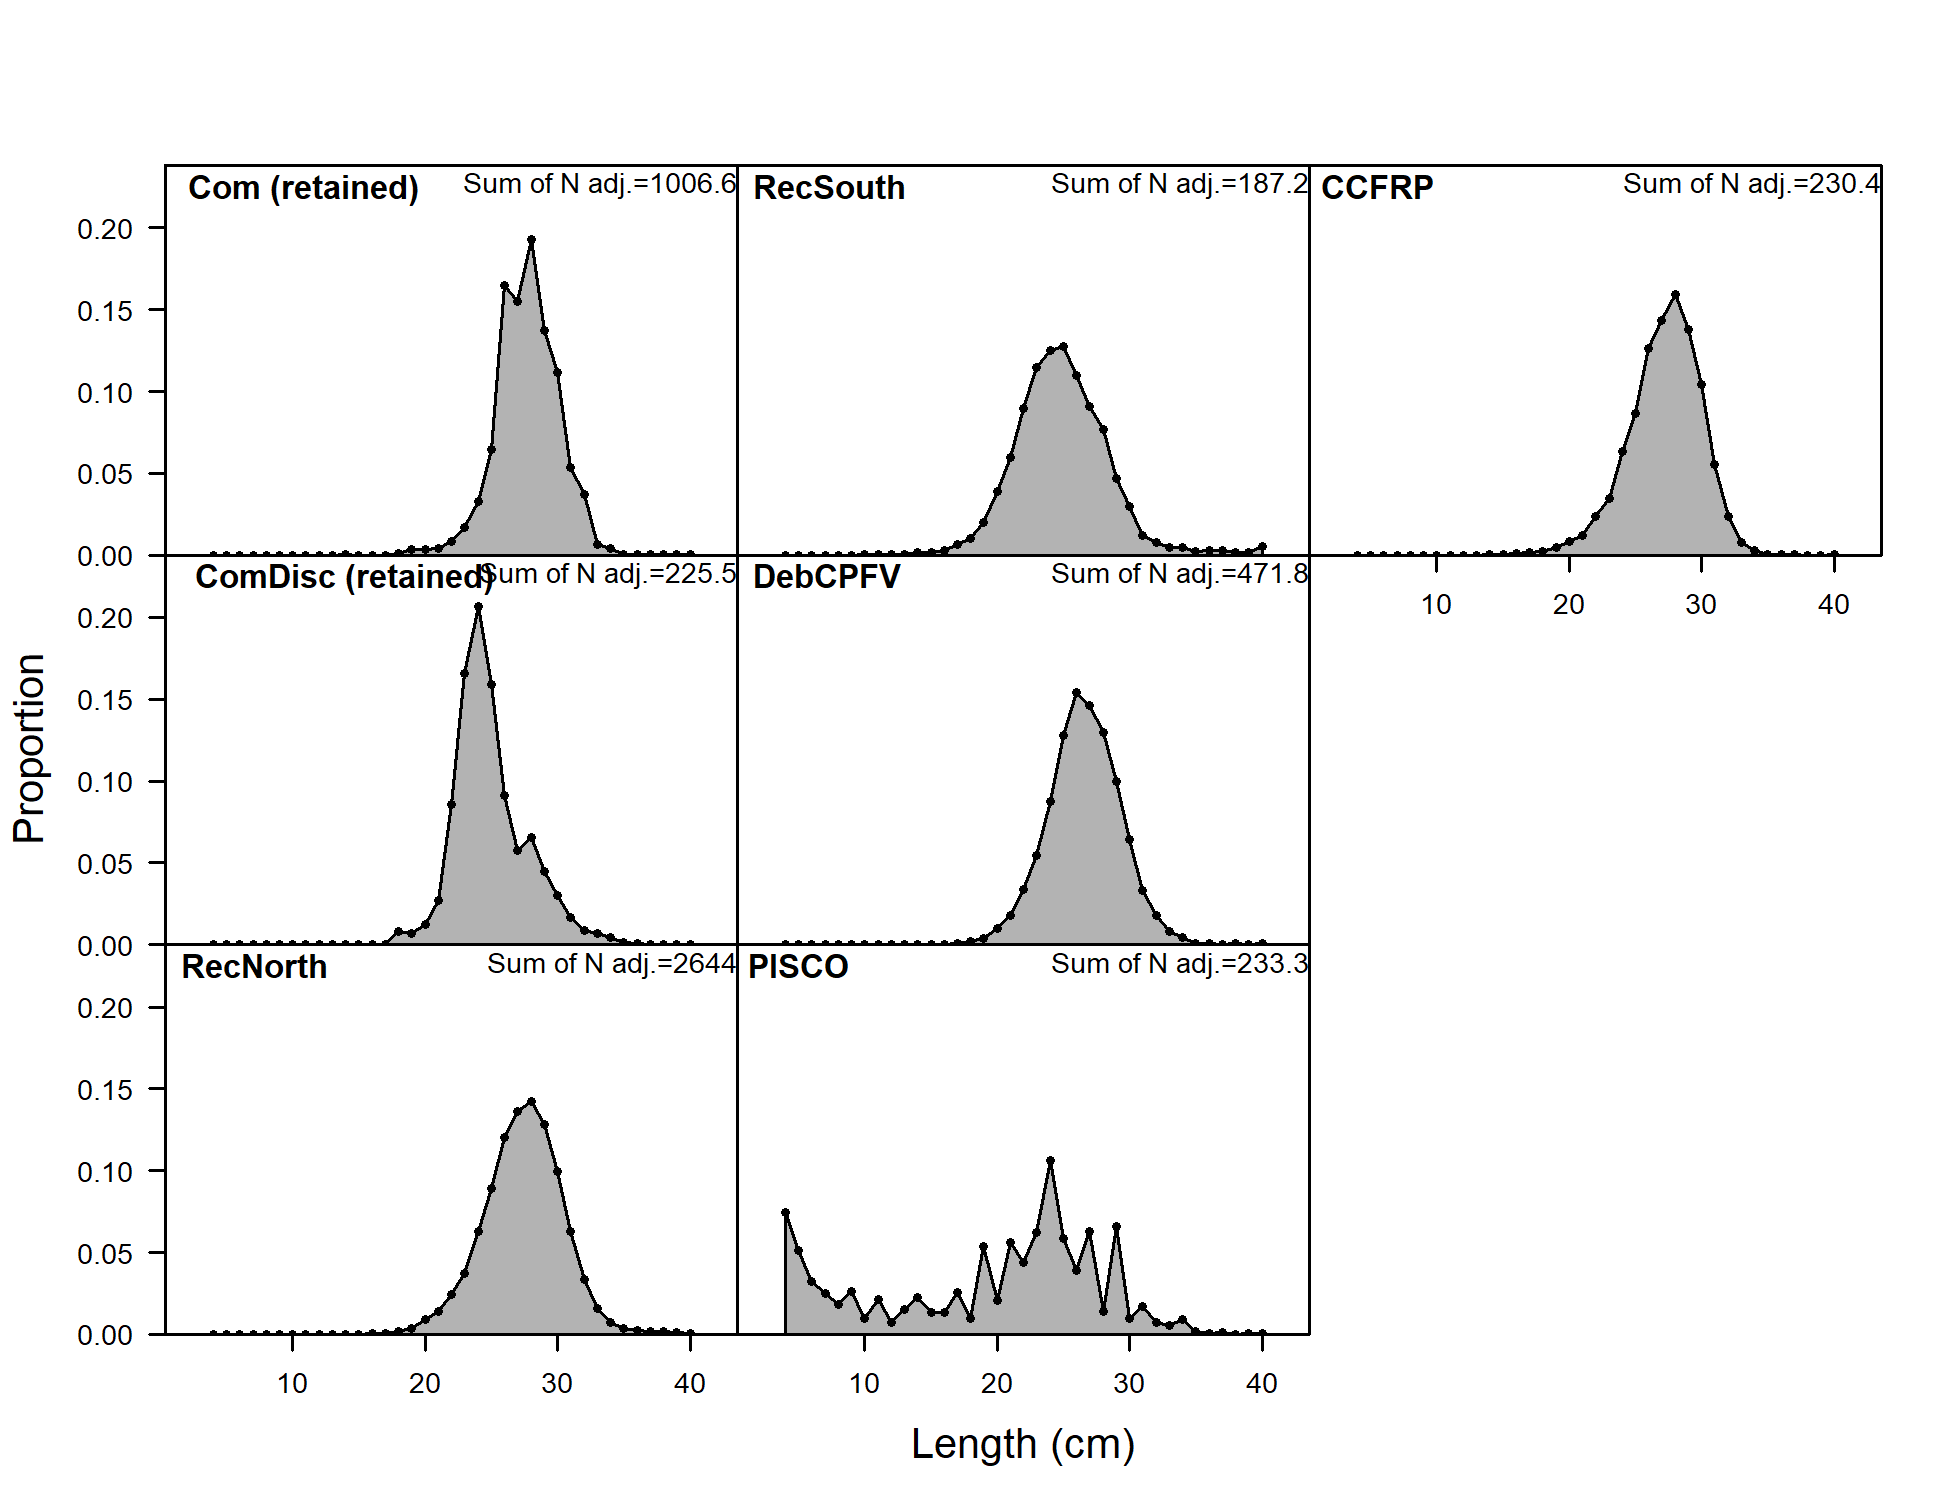
\includegraphics{r4ss/plots_mod1/comp_lendat__aggregated_across_time.png}
\caption{Length comp data, aggregated across time by fleet. Labels
`retained' and `discard' indicate discarded or retained sampled for each
fleet. Panels without this designation represent the whole catch.
\label{fig:comp_lendat_aggregated_across_time}}
\end{figure}

\begin{figure}
\centering
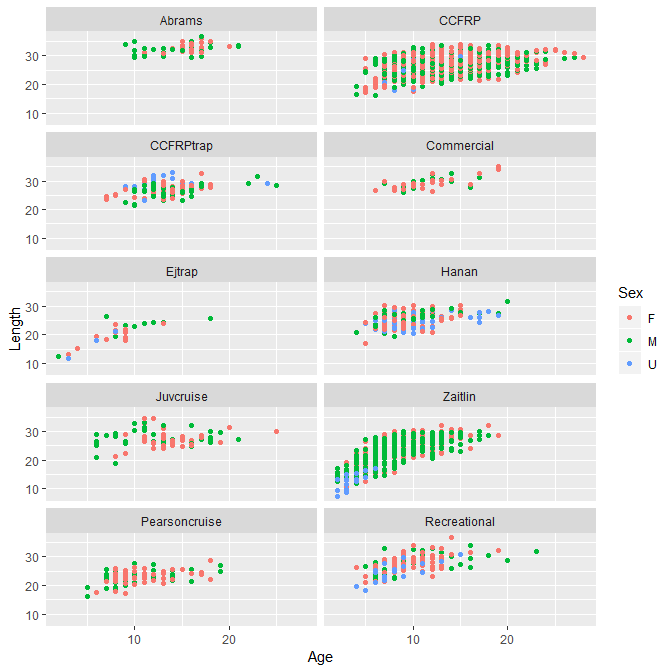
\includegraphics{Figures/Age_length_by_study}
\caption{Available length-at-age data for gopher and black-and-yellow
rockfish by sex and data source. The Zaitlin study is all
black-and-yellow rockfish. The remaining plots represent gopher rockfish
\label{fig:growth_samples}}
\end{figure}

\begin{figure}
\centering
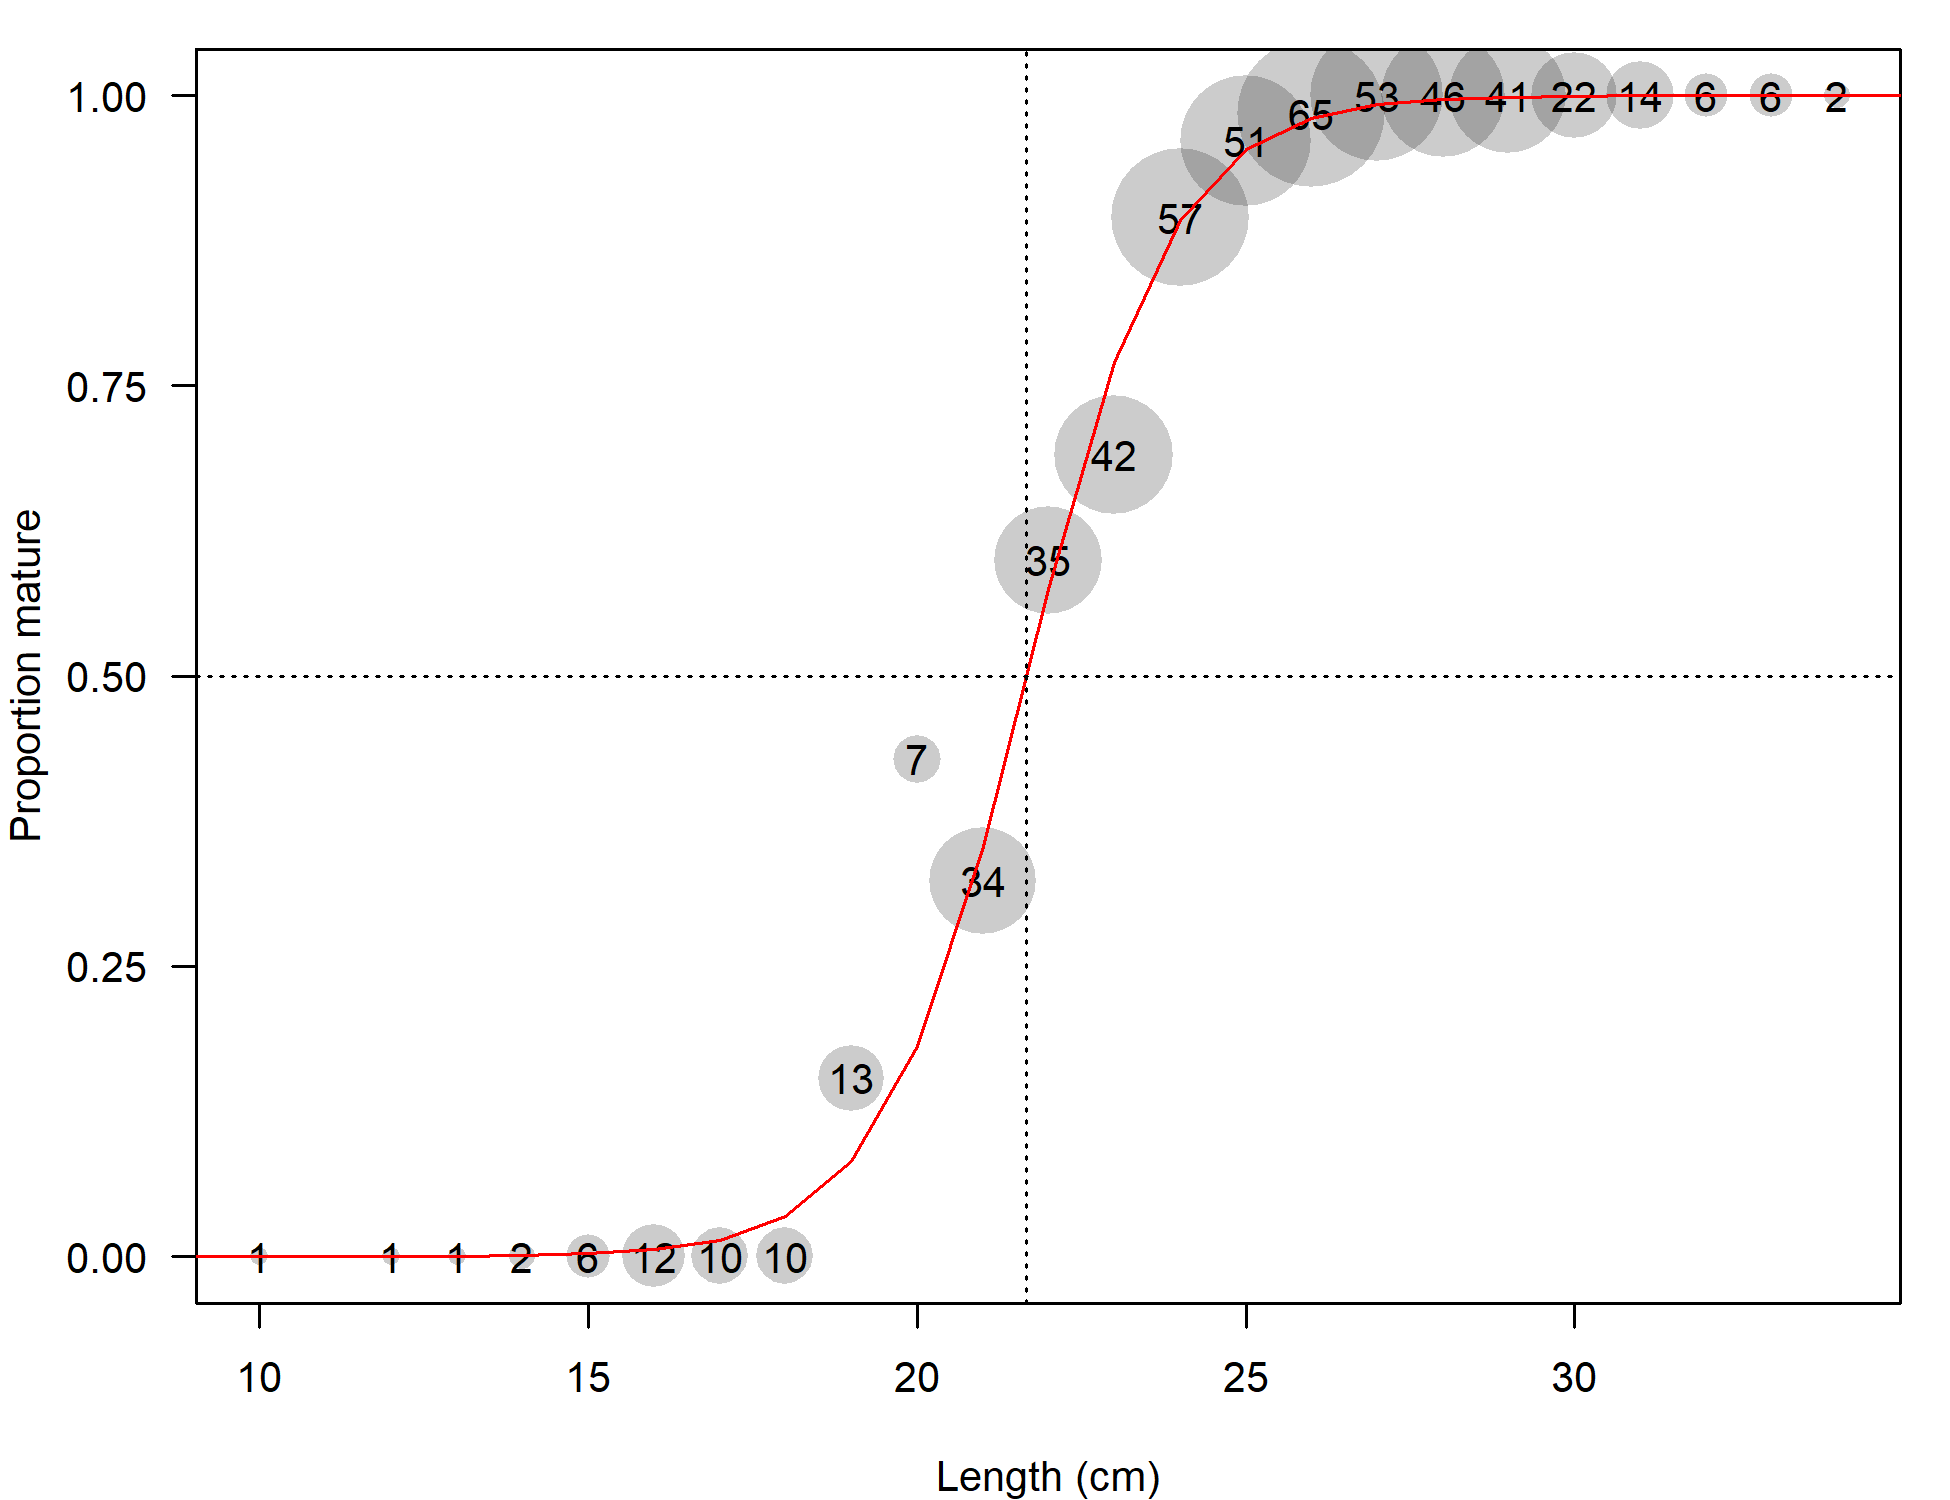
\includegraphics{Figures/GBY_maturity_ogive.png}
\caption{Maturity ogive for females estimated from black-and-yellow
rockfish from Zaitlin (1986) and gopher rockfish from Meyers-Cherry
(2014). Sample sizes at a given length are shown in the circles.
\label{fig:GBY_maturity_ogive}}
\end{figure}

\begin{figure}
\centering
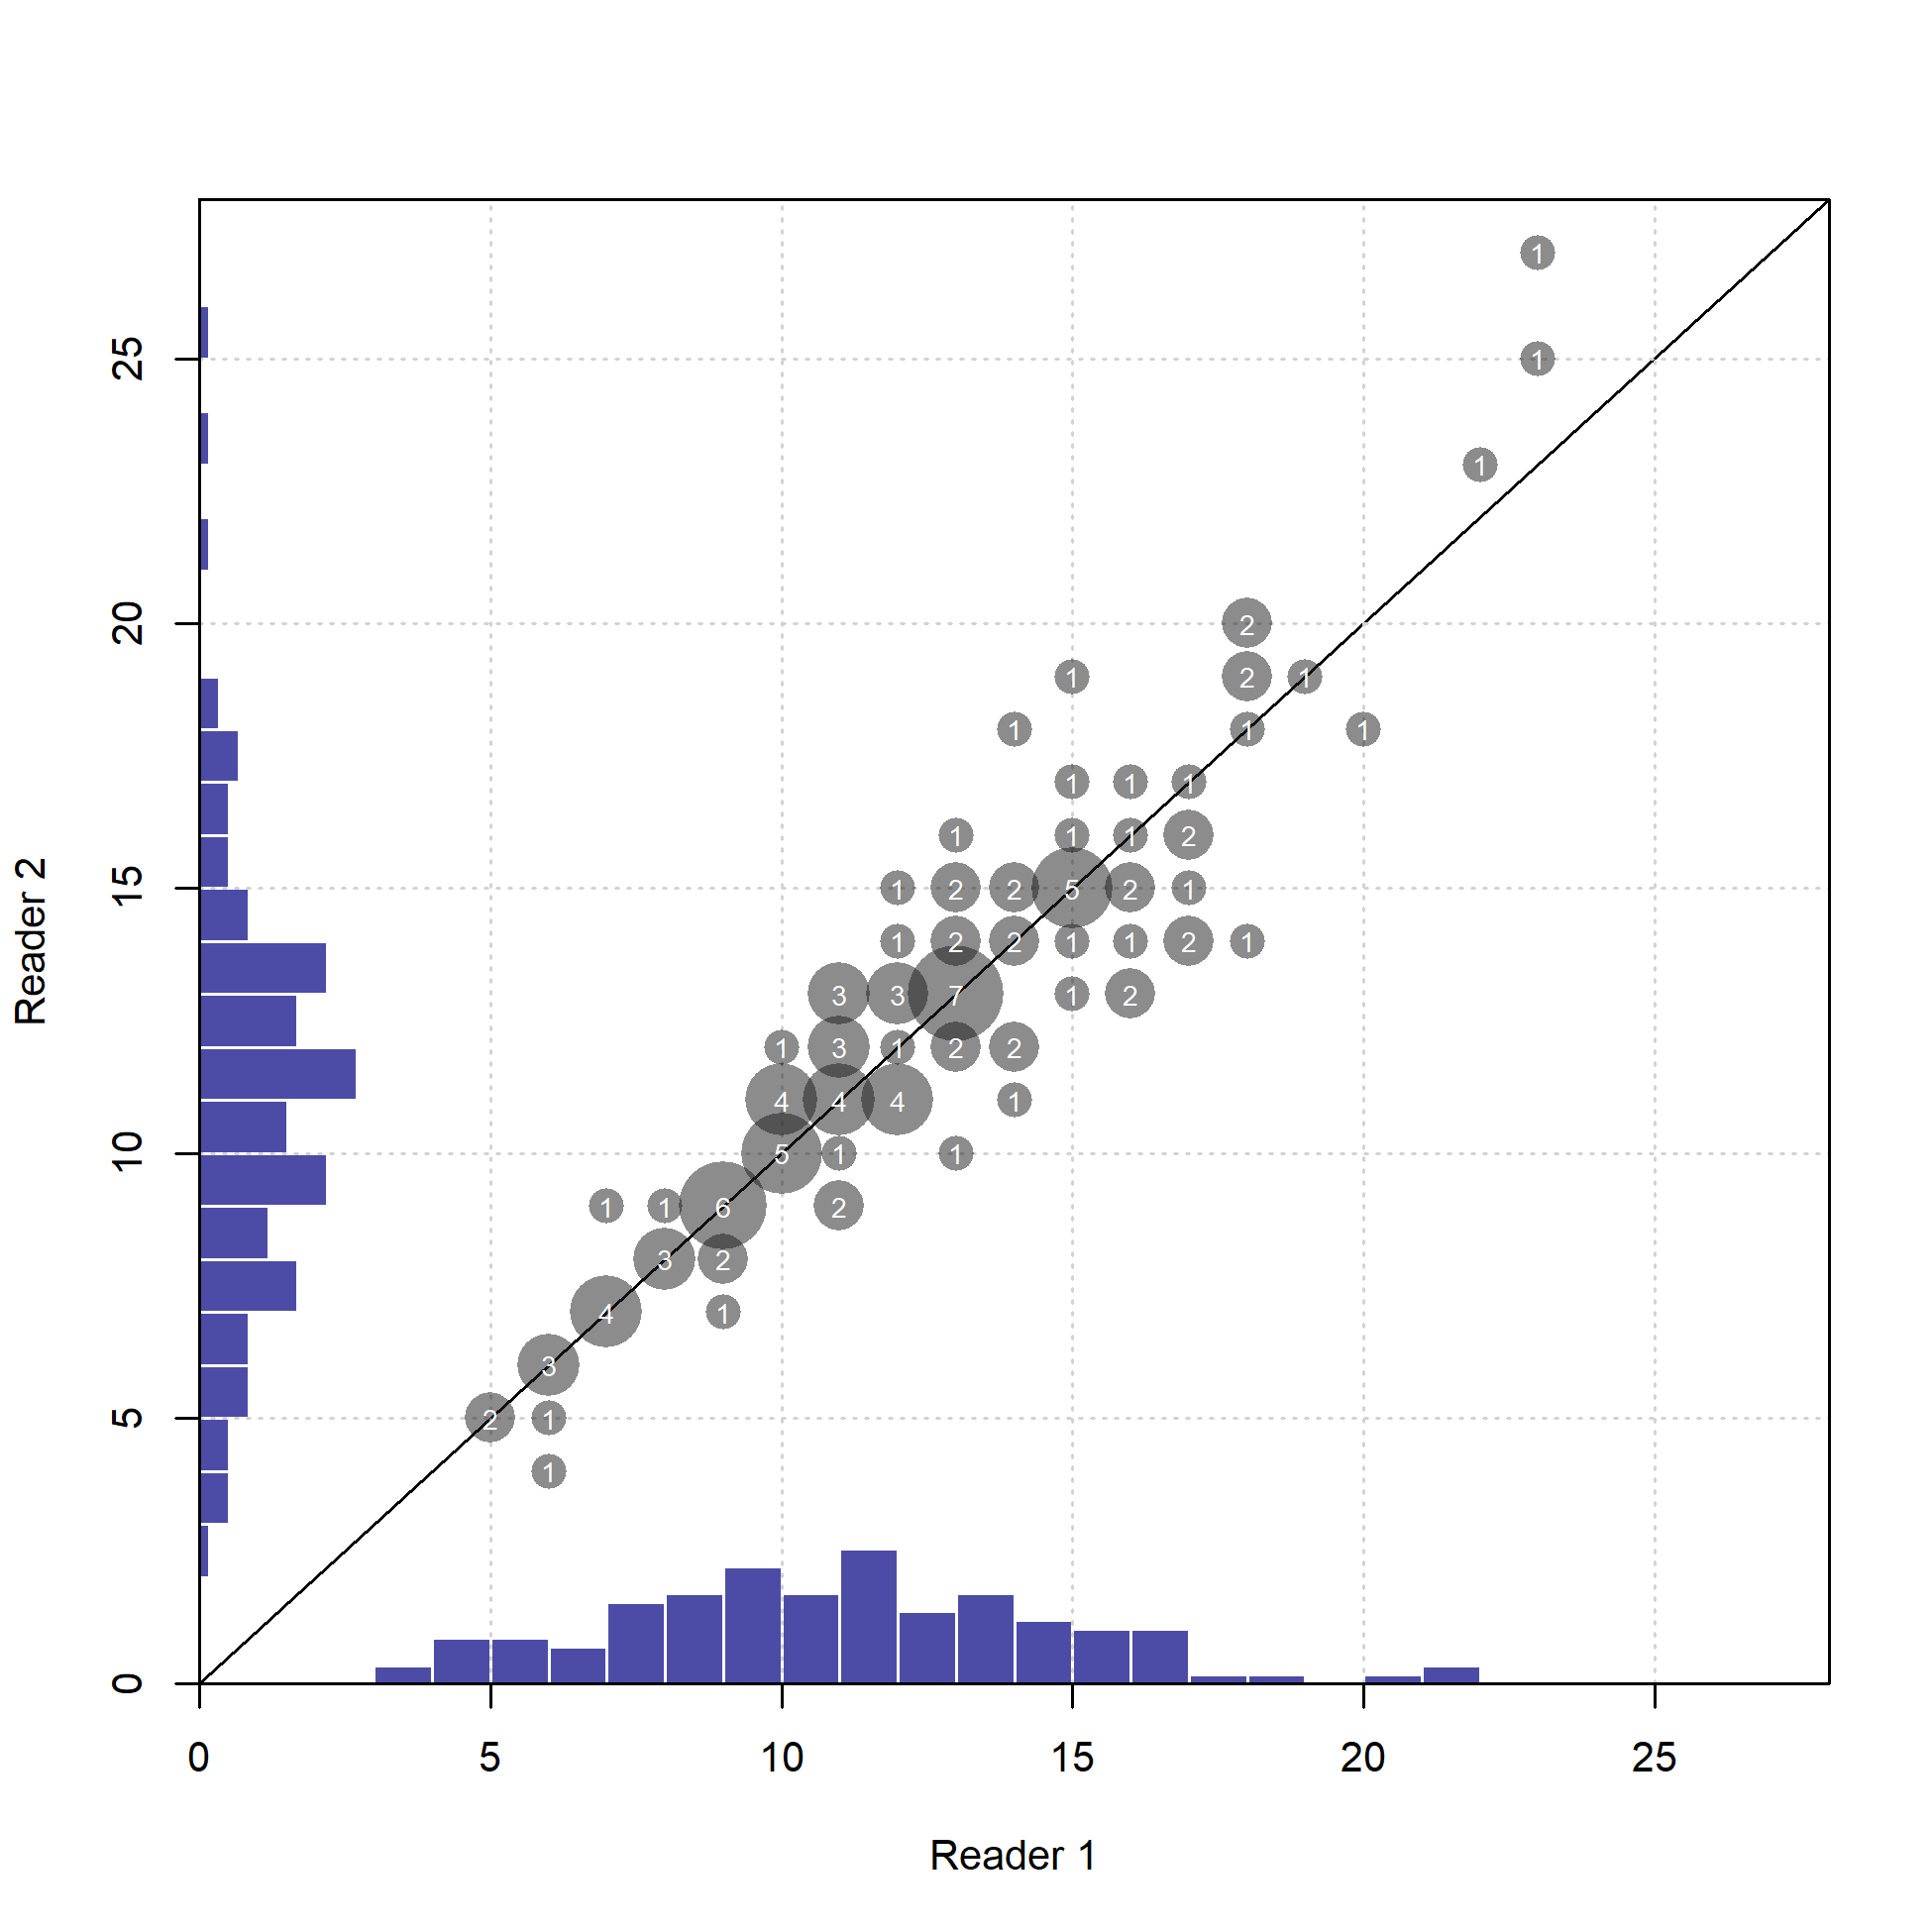
\includegraphics{Figures/GBY_age_error.png}
\caption{Aging precision between initial and blind double reads for
GBYR. Numbers in the bubbles are the sample sizes of otoliths
cross-read. \label{fig:GBY_age_error}}
\end{figure}

\begin{figure}
\centering
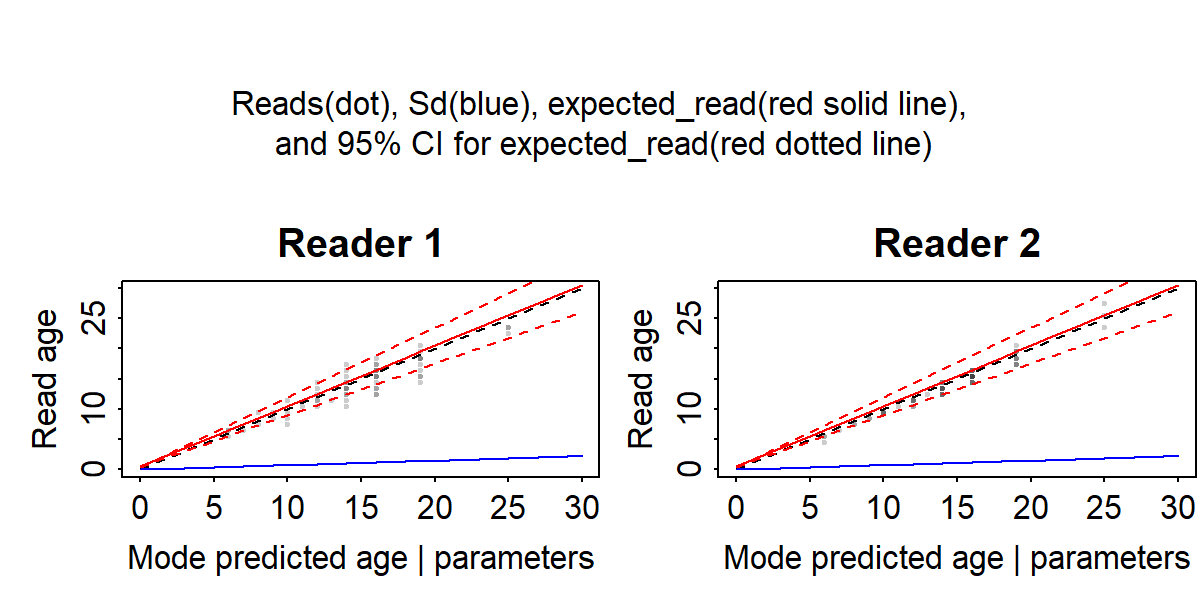
\includegraphics{Figures/GBY_age_error2.png}
\caption{True versus predicted age for two current age readers at the
NWFSC from the ageing error software with unbiased reads and curvilinear
standard deviation for both readers. \label{fig:GBY_age_error2}}
\end{figure}

\begin{figure}
\centering
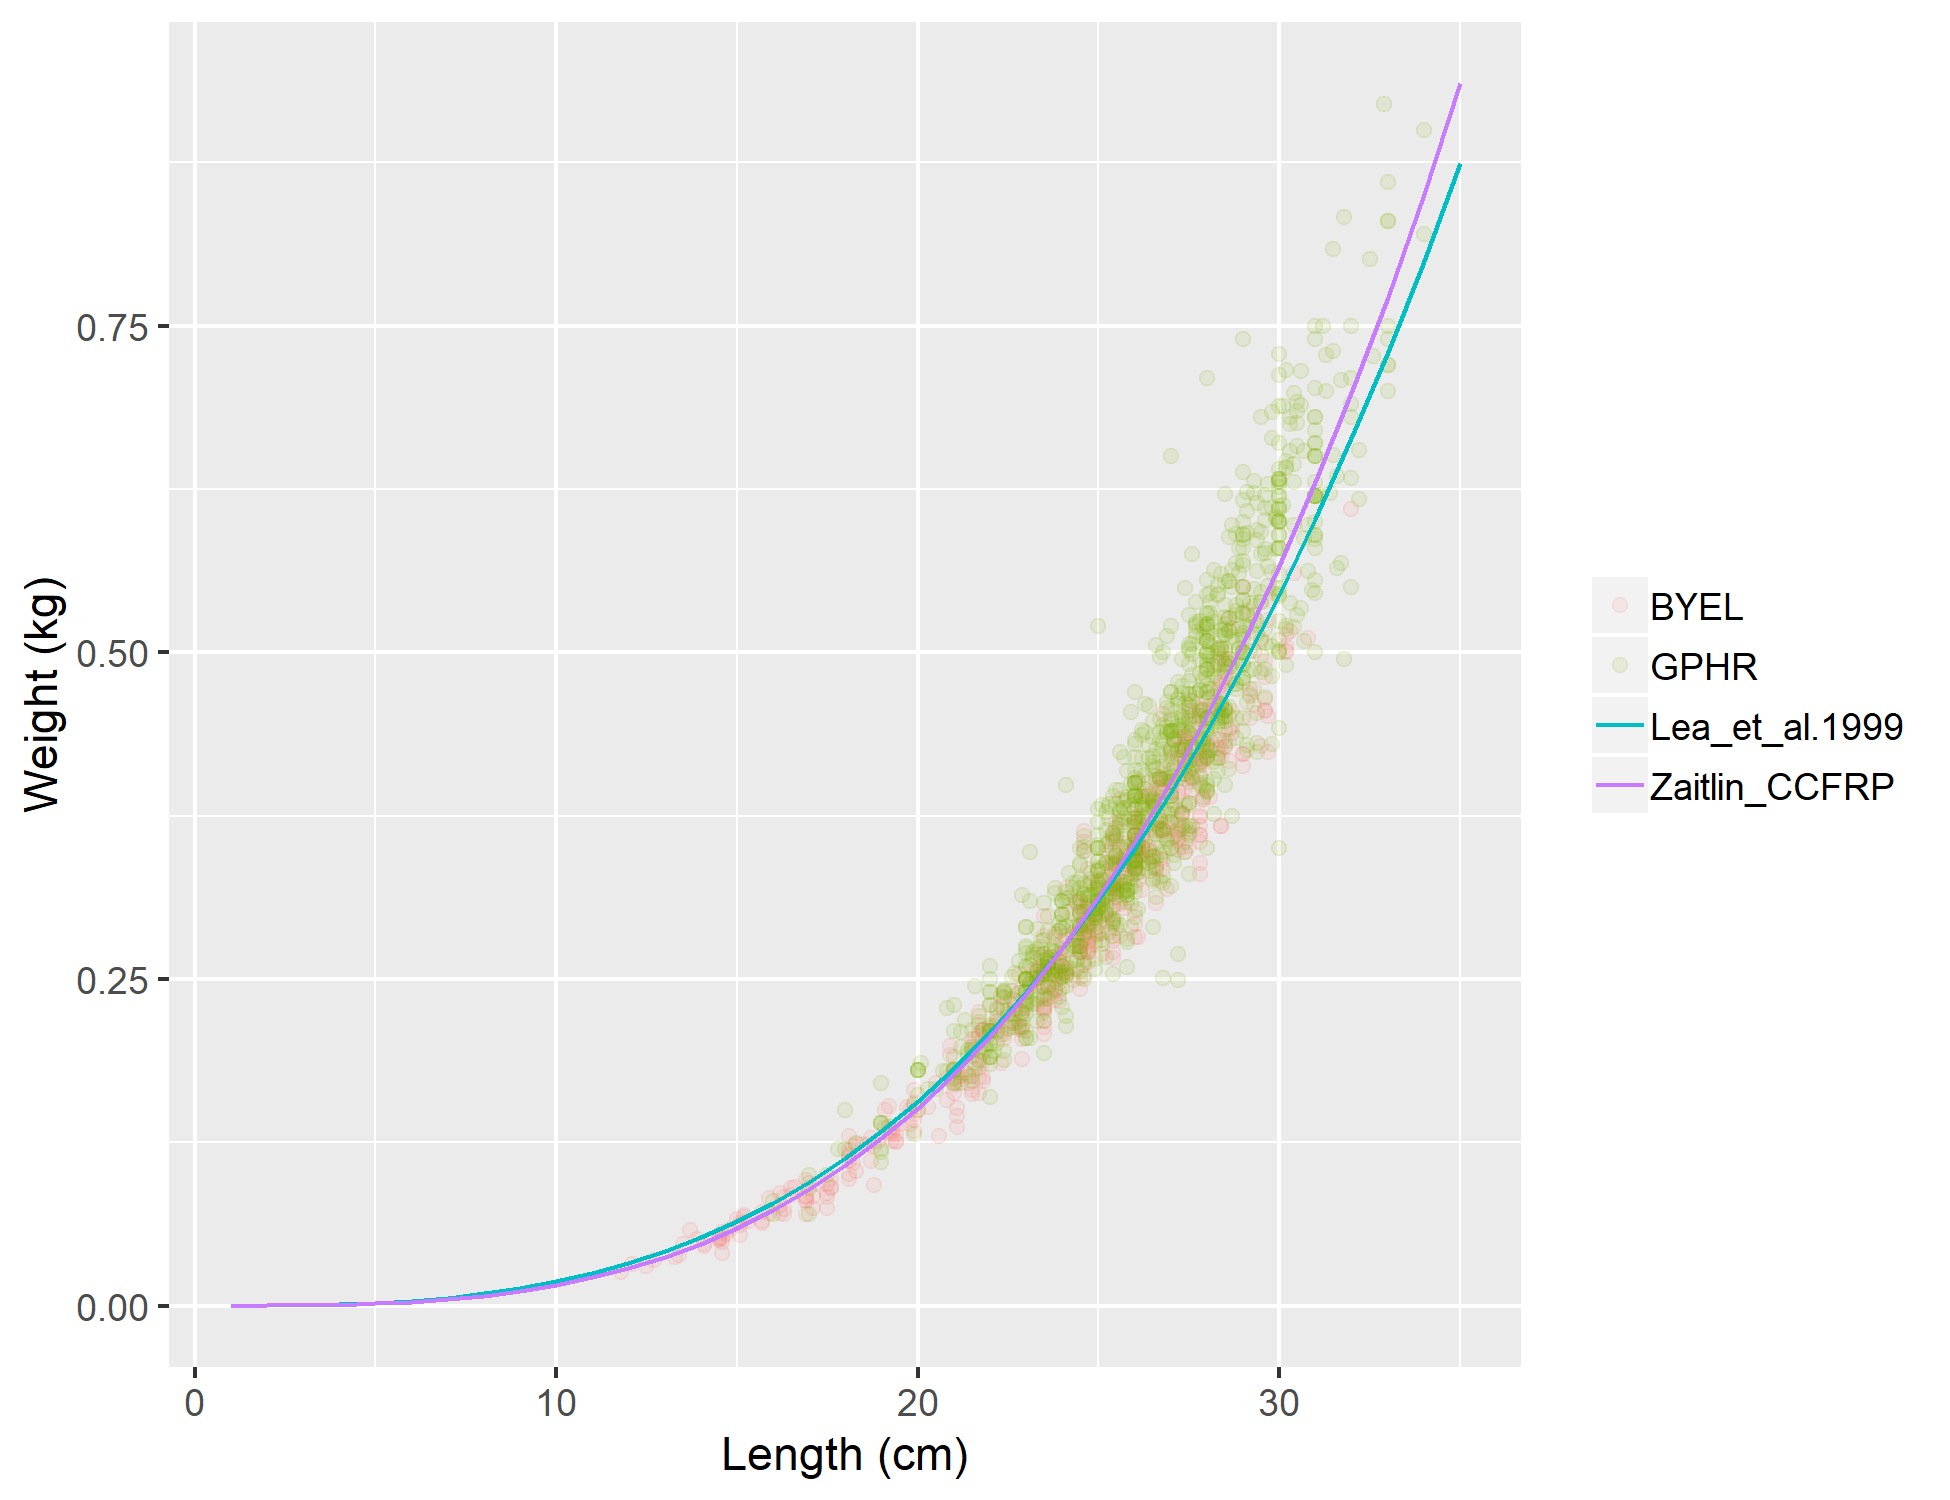
\includegraphics{Figures/GBY_weight_length.png}
\caption{Comparison of the gopher rockfish weight-length curves from Lee
et al. (1999) and tha estimated from black-and-yellow rockfishes from
Zaitlin (1986), and gopher rockfishes from Loury (2011) and
Meyers-Cherry(2014). The estimated curve from the current data is used
in this assessment. \label{fig:GBY_weight_length}}
\end{figure}

\FloatBarrier

\begin{figure}
\centering
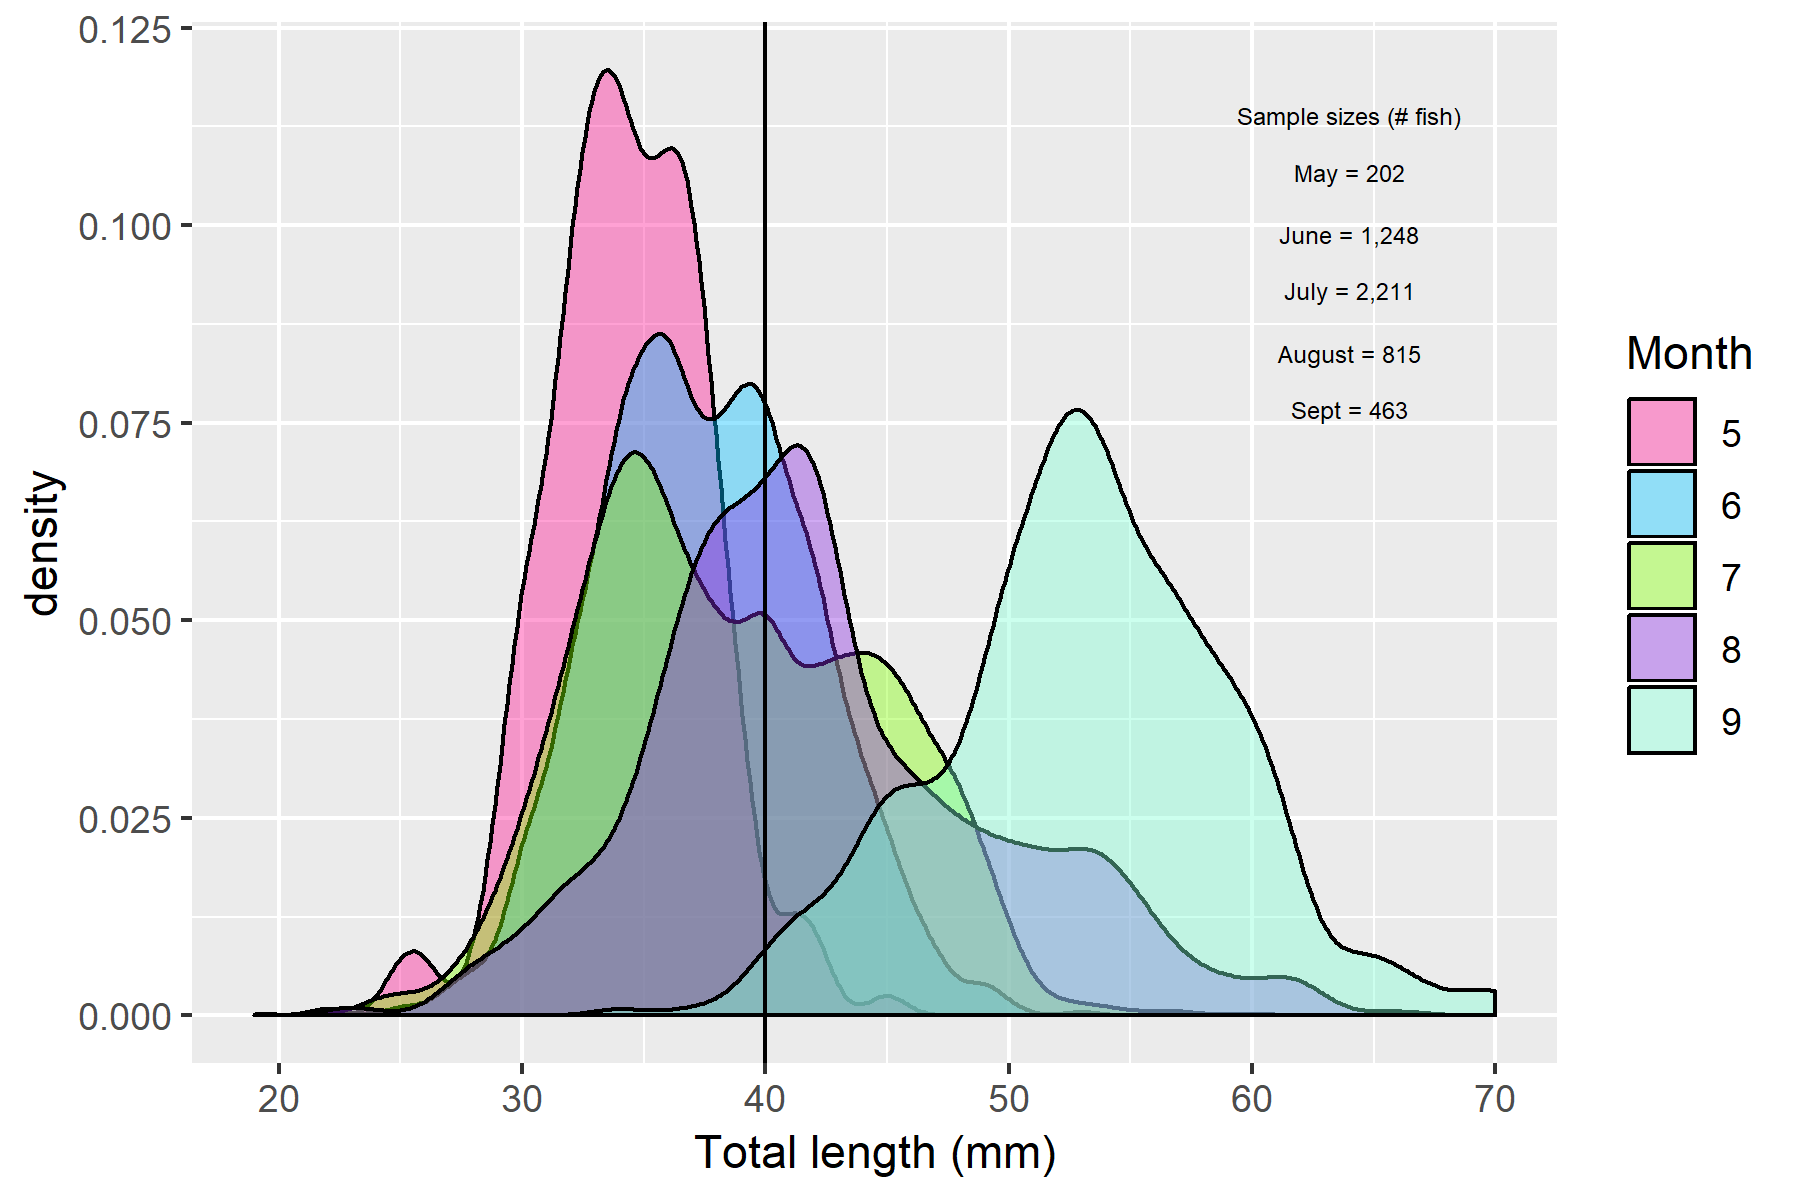
\includegraphics{Figures/SMURF_lengths.png}
\caption{Length distribution by month for GBYR captured using a sampling
toold called a Standard Monitoring Unit for the Recruitment of Fishes
(SMURFs) from the UCSC-PISCO kelp forest fish survey, specifically as
part of Diana Baetscher's dissertation work (Baetscher 2019).
\label{fig:SMURF_lengths}}
\end{figure}

\FloatBarrier

\begin{figure}
\centering
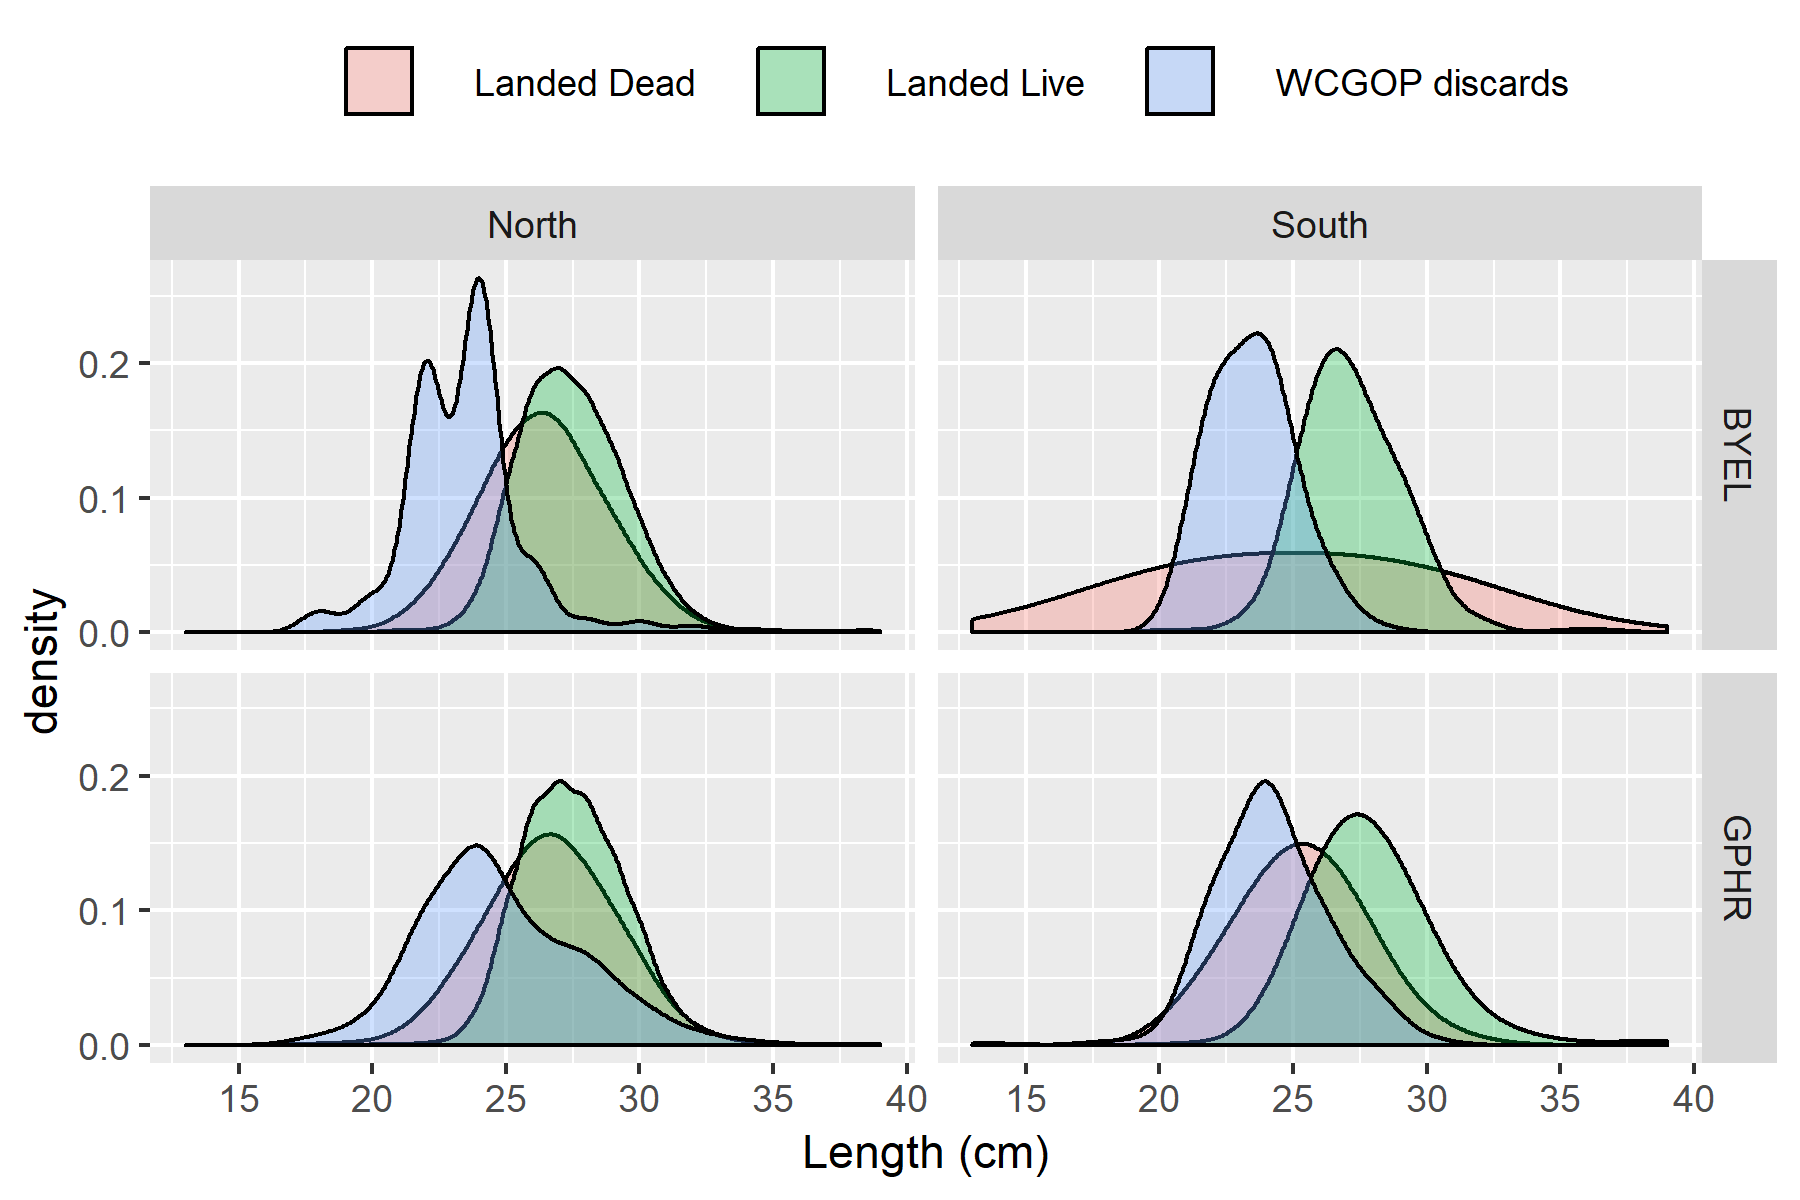
\includegraphics{Figures/Comm_lengths_justification.png}
\caption{Length distributions of gopher and black-and-yellow rockfish
for the commercial fleet and WCGOP discards north and south of Point
Conception. The commercial landings were also separated between fish
landed live and fish landed dead for this figure.
\label{fig:Comm_lengths_justification}}
\end{figure}

\FloatBarrier

\begin{figure}
\centering
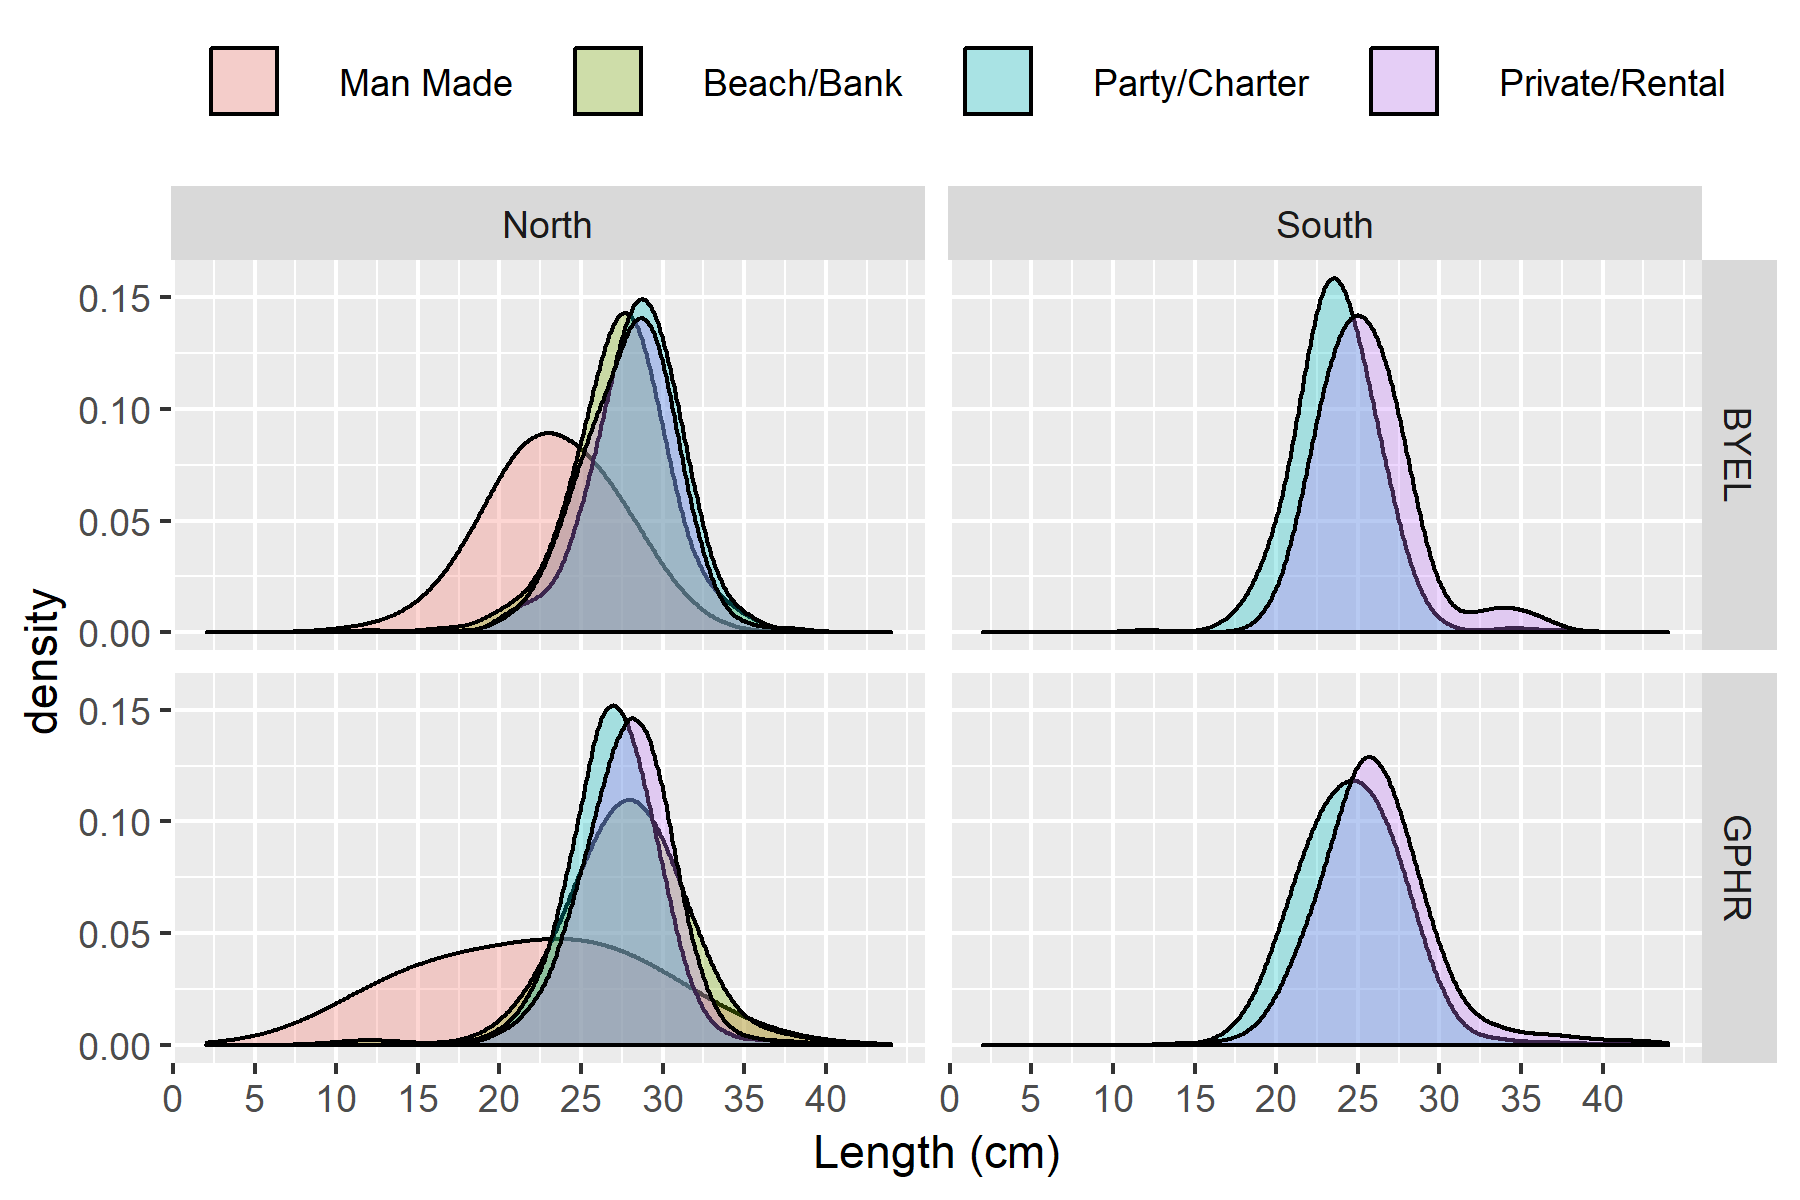
\includegraphics{Figures/Rec_lengths_justification.png}
\caption{Length distributions of gopher and black-and-yellow rockfish
for the recreational fleet north and south of Point Conception and by
mode. \label{fig:Rec_lengths_justification}}
\end{figure}

\FloatBarrier

\FloatBarrier

\begin{figure}
\centering
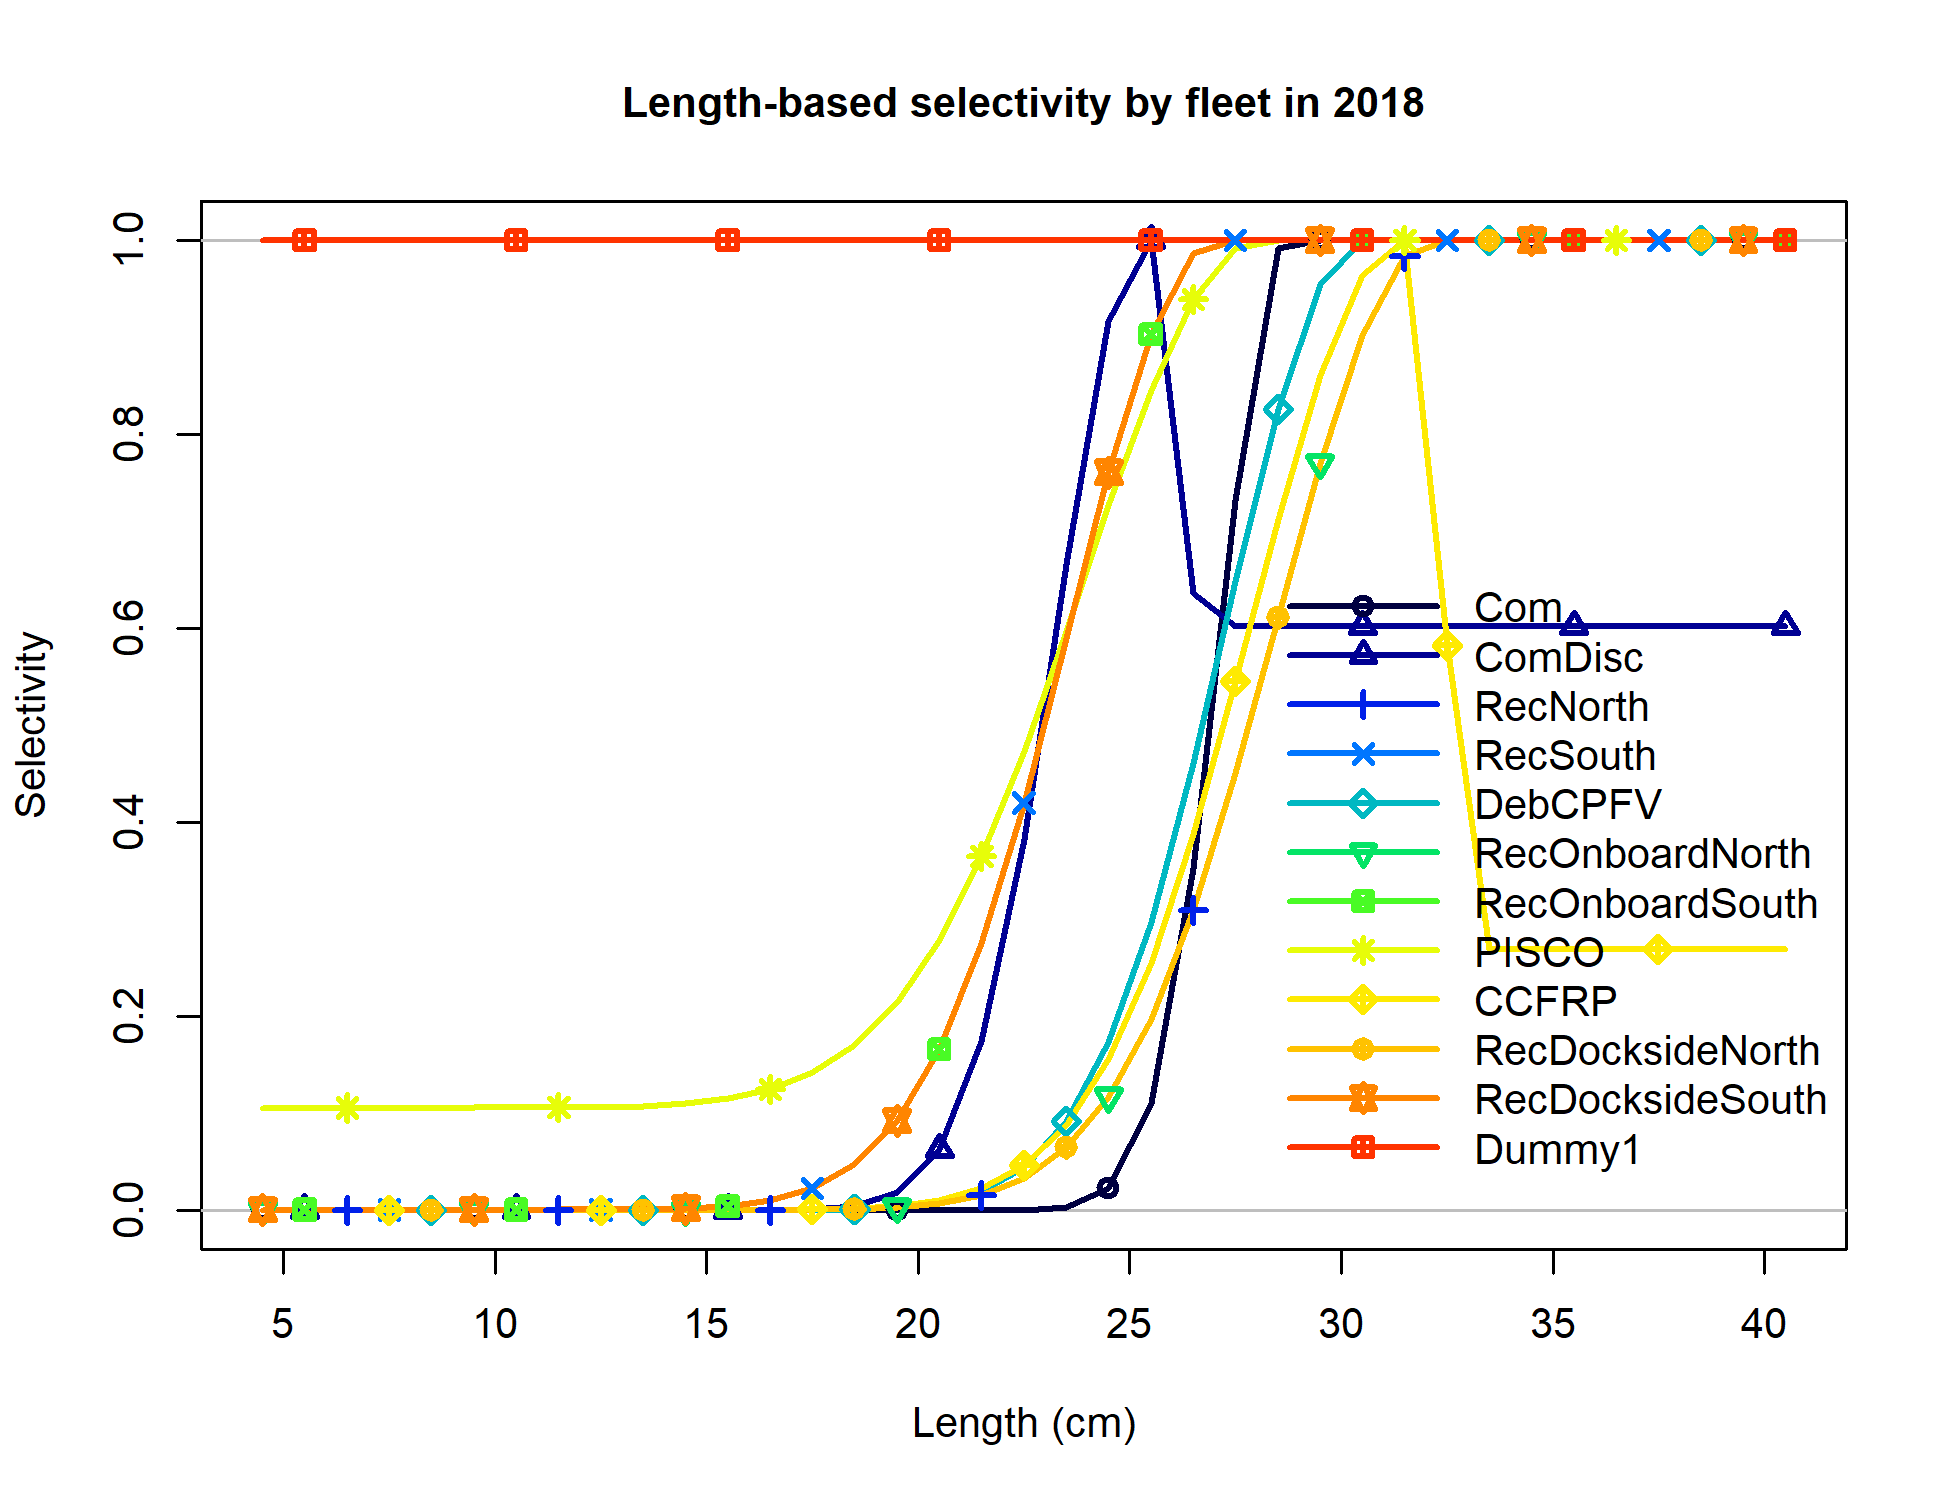
\includegraphics{r4ss/plots_mod1/sel01_multiple_fleets_length1.png}
\caption{Selectivity at length for all of the fleets in the base model.
\label{fig:sel01_multiple_fleets_length1}}
\end{figure}

\FloatBarrier

\begin{figure}
\centering
\includegraphics{r4ss/plots_mod1/ts11_Age-0_recruits_(1000s)_with_95_asymptotic_intervals.png}
\caption{Time series of estimated GBYR recruitments for the base-case
model with 95\% confidence or credibility intervals.
\label{fig:Recruit_mod1}}
\end{figure}

\begin{figure}
\centering
\includegraphics{r4ss/plots_mod1/SR_curve2.png}
\caption{Estimated recruitment (red circles) and the assumed
stock-recruit relationship (black line) for GBYR. The green line shows
the effect of the bias correction for the lognormal distribution.
\label{fig:SR_curve2}}
\end{figure}

\FloatBarrier

\begin{figure}
\centering
\includegraphics{./r4ss/plots_mod1/comp_condAALfit_residsflt12mkt0.png}
\caption{Pearson residuals, whole catch, Dummy1 (max=22.55)
\label{fig:mod1_4_comp_condAALfit_residsflt12mkt0}}
\end{figure}

\begin{figure}
\centering
\includegraphics{./r4ss/plots_mod1/comp_condAALfit_data_weighting_TA1.8_condAgeCom.png}
\caption{Mean age from conditional data (aggregated across length bins)
for Com with 95\% confidence intervals based on current samples sizes.
Francis data weighting method TA1.8: thinner intervals (with capped
ends) show result of further adjusting sample sizes based on suggested
multiplier (with 95\% interval) for conditional age\_at\_length data
from Com: 1.0859 (0.6193\_33.7322) For more info, see Francis, R.I.C.C.
(2011). Data weighting in statistical fisheries stock assessment models.
Can. J. Fish. Aquat. Sci. 68: 1124\_1138.
\label{fig:mod1_5_comp_condAALfit_data_weighting_TA1.8_condAgeCom}}
\end{figure}

\begin{figure}
\centering
\includegraphics{./r4ss/plots_mod1/comp_condAALfit_Andre_plotsflt1mkt0_page1.png}
\caption{Conditional AAL plot, whole catch, Com (plot 1 of 2) These
plots show mean age and std. dev. in conditional AAL. Left plots are
mean AAL by size\_class (obs. and pred.) with 90\% CIs based on adding
1.64 SE of mean to the data. Right plots in each pair are SE of mean AAL
(obs. and pred.) with 90\% CIs based on the chi\_square distribution.
\label{fig:mod1_6_comp_condAALfit_Andre_plotsflt1mkt0_page1}}
\end{figure}

\includegraphics{./r4ss/plots_mod1/comp_condAALfit_Andre_plotsflt1mkt0_page2.png}

\begin{center} 

              Figure continued from previous page 

             \end{center}

\begin{figure}
\centering
\includegraphics{./r4ss/plots_mod1/comp_condAALfit_data_weighting_TA1.8_condAgeRecNorth.png}
\caption{Mean age from conditional data (aggregated across length bins)
for RecNorth with 95\% confidence intervals based on current samples
sizes. Francis data weighting method TA1.8: thinner intervals (with
capped ends) show result of further adjusting sample sizes based on
suggested multiplier (with 95\% interval) for conditional
age\_at\_length data from RecNorth: 0.8677 (0.589\_3.1055) For more
info, see Francis, R.I.C.C. (2011). Data weighting in statistical
fisheries stock assessment models. Can. J. Fish. Aquat. Sci. 68:
1124\_1138.
\label{fig:mod1_8_comp_condAALfit_data_weighting_TA1.8_condAgeRecNorth}}
\end{figure}

\begin{figure}
\centering
\includegraphics{./r4ss/plots_mod1/comp_condAALfit_Andre_plotsflt3mkt0_page1.png}
\caption{Conditional AAL plot, whole catch, RecNorth (plot 1 of 3) These
plots show mean age and std. dev. in conditional AAL. Left plots are
mean AAL by size\_class (obs. and pred.) with 90\% CIs based on adding
1.64 SE of mean to the data. Right plots in each pair are SE of mean AAL
(obs. and pred.) with 90\% CIs based on the chi\_square distribution.
\label{fig:mod1_9_comp_condAALfit_Andre_plotsflt3mkt0_page1}}
\end{figure}

\includegraphics{./r4ss/plots_mod1/comp_condAALfit_Andre_plotsflt3mkt0_page2.png}

\begin{center} 

              Figure continued from previous page 

             \end{center}

\includegraphics{./r4ss/plots_mod1/comp_condAALfit_Andre_plotsflt3mkt0_page3.png}

\begin{center} 

              Figure continued from previous page 

             \end{center}

\begin{figure}
\centering
\includegraphics{./r4ss/plots_mod1/comp_condAALfit_data_weighting_TA1.8_condAgeCCFRP.png}
\caption{Mean age from conditional data (aggregated across length bins)
for CCFRP with 95\% confidence intervals based on current samples sizes.
Francis data weighting method TA1.8: thinner intervals (with capped
ends) show result of further adjusting sample sizes based on suggested
multiplier (with 95\% interval) for conditional age\_at\_length data
from CCFRP: 0.5645 (0.344\_2.4444) For more info, see Francis, R.I.C.C.
(2011). Data weighting in statistical fisheries stock assessment models.
Can. J. Fish. Aquat. Sci. 68: 1124\_1138.
\label{fig:mod1_12_comp_condAALfit_data_weighting_TA1.8_condAgeCCFRP}}
\end{figure}

\begin{figure}
\centering
\includegraphics{./r4ss/plots_mod1/comp_condAALfit_Andre_plotsflt9mkt0_page1.png}
\caption{Conditional AAL plot, whole catch, CCFRP (plot 1 of 3) These
plots show mean age and std. dev. in conditional AAL. Left plots are
mean AAL by size\_class (obs. and pred.) with 90\% CIs based on adding
1.64 SE of mean to the data. Right plots in each pair are SE of mean AAL
(obs. and pred.) with 90\% CIs based on the chi\_square distribution.
\label{fig:mod1_13_comp_condAALfit_Andre_plotsflt9mkt0_page1}}
\end{figure}

\includegraphics{./r4ss/plots_mod1/comp_condAALfit_Andre_plotsflt9mkt0_page2.png}

\begin{center} 

              Figure continued from previous page 

             \end{center}

\includegraphics{./r4ss/plots_mod1/comp_condAALfit_Andre_plotsflt9mkt0_page3.png}

\begin{center} 

              Figure continued from previous page 

             \end{center}

\begin{figure}
\centering
\includegraphics{./r4ss/plots_mod1/comp_condAALfit_data_weighting_TA1.8_condAgeDummy1.png}
\caption{Mean age from conditional data (aggregated across length bins)
for Dummy1 with 95\% confidence intervals based on current samples
sizes. Francis data weighting method TA1.8: thinner intervals (with
capped ends) show result of further adjusting sample sizes based on
suggested multiplier (with 95\% interval) for conditional
age\_at\_length data from Dummy1: 0.6218 (0.324\_3.077) For more info,
see Francis, R.I.C.C. (2011). Data weighting in statistical fisheries
stock assessment models. Can. J. Fish. Aquat. Sci. 68: 1124\_1138.
\label{fig:mod1_16_comp_condAALfit_data_weighting_TA1.8_condAgeDummy1}}
\end{figure}

\begin{figure}
\centering
\includegraphics{./r4ss/plots_mod1/comp_condAALfit_Andre_plotsflt12mkt0_page1.png}
\caption{Conditional AAL plot, whole catch, Dummy1 (plot 1 of 5) These
plots show mean age and std. dev. in conditional AAL. Left plots are
mean AAL by size\_class (obs. and pred.) with 90\% CIs based on adding
1.64 SE of mean to the data. Right plots in each pair are SE of mean AAL
(obs. and pred.) with 90\% CIs based on the chi\_square distribution.
\label{fig:mod1_17_comp_condAALfit_Andre_plotsflt12mkt0_page1}}
\end{figure}

\includegraphics{./r4ss/plots_mod1/comp_condAALfit_Andre_plotsflt12mkt0_page2.png}

\begin{center} 

              Figure continued from previous page 

             \end{center}

\includegraphics{./r4ss/plots_mod1/comp_condAALfit_Andre_plotsflt12mkt0_page3.png}

\begin{center} 

              Figure continued from previous page 

             \end{center}

\includegraphics{./r4ss/plots_mod1/comp_condAALfit_Andre_plotsflt12mkt0_page4.png}

\begin{center} 

              Figure continued from previous page 

             \end{center}

\includegraphics{./r4ss/plots_mod1/comp_condAALfit_Andre_plotsflt12mkt0_page5.png}

\begin{center} 

              Figure continued from previous page 

             \end{center}

\FloatBarrier

\FloatBarrier

\FloatBarrier
<!-- ***********h Likelihood profile FIGURES******************************* -->

\FloatBarrier
<!-- ********************************************************************** -->

\begin{figure}
\centering
\includegraphics{r4ss/plots_mod1/ts7_Spawning_output_with_95_asymptotic_intervals_intervals.png}
\caption{Estimated spawning biomass (mt) with approximate 95\%
asymptotic intervals.
\label{fig:ts7_Spawning_biomass_(mt)_with_95_asymptotic_intervals_intervals}}
\end{figure}

\begin{figure}
\centering
\includegraphics{r4ss/plots_mod1/ts9_unfished_with_95_asymptotic_intervals_intervals.png}
\caption{Estimated spawning depletion with approximate 95\% asymptotic
intervals.
\label{fig:ts9_unfished_with_95_asymptotic_intervals_intervals}}
\end{figure}

\begin{figure}
\centering
\includegraphics{r4ss/plots_mod1/yield1_yield_curve.png}
\caption{Equilibrium yield curve for the base case model. Values are
based on the 2018 fishery selectivity and with steepness fixed at 0.718.
\label{fig:yield1_yield_curve}}
\end{figure}

\FloatBarrier
<!-- ********************************************************************** -->

\FloatBarrier
\newpage

\hypertarget{appendix-a.-californias-commercial-fishery-regulations}{\section*{Appendix
A. California's Commercial Fishery
Regulations}\label{appendix-a.-californias-commercial-fishery-regulations}}
\addcontentsline{toc}{section}{Appendix A. California's Commercial
Fishery Regulations}

\renewcommand{\thepage}{A-\arabic{page}}
\renewcommand{\thefigure}{A\arabic{figure}}

\setcounter{page}{1} \setcounter{figure}{1}

\begin{figure}
\centering
\includegraphics{Figures/Comm_regs1.pdf}
\caption{\label{fig:Comm_regs1}}
\end{figure}

\FloatBarrier

\begin{figure}
\centering
\includegraphics{Figures/Comm_regs2.pdf}
\caption{\label{fig:Comm_regs2}}
\end{figure}

\FloatBarrier

\begin{figure}
\centering
\includegraphics{Figures/Comm_regs3.pdf}
\caption{\label{fig:Comm_regs3}}
\end{figure}

\FloatBarrier
\newpage

\hypertarget{appendix-b.-californias-recreational-fishery-regulations}{\section*{Appendix
B. California's Recreational Fishery
Regulations}\label{appendix-b.-californias-recreational-fishery-regulations}}
\addcontentsline{toc}{section}{Appendix B. California's Recreational
Fishery Regulations}

\renewcommand{\thepage}{B-\arabic{page}}
\renewcommand{\thefigure}{B\arabic{figure}}

\setcounter{page}{1} \setcounter{figure}{1}

\begin{figure}
\centering
\includegraphics{Figures/Rec_regs1.pdf}
\caption{\label{fig:Rec_regs1}}
\end{figure}

\FloatBarrier

\begin{figure}
\centering
\includegraphics{Figures/Rec_regs2.pdf}
\caption{\label{fig:Rec_regs2}}
\end{figure}

\FloatBarrier

\begin{figure}
\centering
\includegraphics{Figures/Rec_regs3.pdf}
\caption{\label{fig:Rec_regs3}}
\end{figure}

\FloatBarrier

\begin{figure}
\centering
\includegraphics{Figures/Rec_regs4.pdf}
\caption{\label{fig:Rec_reg4}}
\end{figure}

\FloatBarrier
\newpage

\section*{Appendix C. Detailed fits to length composition
data}\label{appendix-c.-detailed-fits-to-length-composition-data}
\addcontentsline{toc}{section}{Appendix C. Detailed fits to length
composition data}

\renewcommand{\thepage}{C-\arabic{page}}
\renewcommand{\thefigure}{C\arabic{figure}}

\setcounter{page}{1} \setcounter{figure}{1}

\begin{figure}
\centering
\includegraphics{./r4ss/plots_mod1/comp_lenfit_flt1mkt2.png}
\caption{Length comps, retained, Com. `N adj.' is the input sample size
after data\_weighting adjustment. N eff. is the calculated effective
sample size used in the McAllister\_Iannelli tuning method.
\label{fig:mod1_1_comp_lenfit_flt1mkt2}}
\end{figure}

\begin{figure}
\centering
\includegraphics{./r4ss/plots_mod1/comp_lenfit_flt2mkt2.png}
\caption{Length comps, retained, ComDisc. `N adj.' is the input sample
size after data\_weighting adjustment. N eff. is the calculated
effective sample size used in the McAllister\_Iannelli tuning method.
\label{fig:mod1_2_comp_lenfit_flt2mkt2}}
\end{figure}

\begin{figure}
\centering
\includegraphics{./r4ss/plots_mod1/comp_lenfit_flt3mkt0.png}
\caption{Length comps, whole catch, RecNorth. `N adj.' is the input
sample size after data\_weighting adjustment. N eff. is the calculated
effective sample size used in the McAllister\_Iannelli tuning method.
\label{fig:mod1_3_comp_lenfit_flt3mkt0}}
\end{figure}

\begin{figure}
\centering
\includegraphics{./r4ss/plots_mod1/comp_lenfit_flt4mkt0.png}
\caption{Length comps, whole catch, RecSouth. `N adj.' is the input
sample size after data\_weighting adjustment. N eff. is the calculated
effective sample size used in the McAllister\_Iannelli tuning method.
\label{fig:mod1_4_comp_lenfit_flt4mkt0}}
\end{figure}

\begin{figure}
\centering
\includegraphics{./r4ss/plots_mod1/comp_lenfit_flt5mkt0.png}
\caption{Length comps, whole catch, DebCPFV. `N adj.' is the input
sample size after data\_weighting adjustment. N eff. is the calculated
effective sample size used in the McAllister\_Iannelli tuning method.
\label{fig:mod1_5_comp_lenfit_flt5mkt0}}
\end{figure}

\begin{figure}
\centering
\includegraphics{./r4ss/plots_mod1/comp_lenfit_flt8mkt0.png}
\caption{Length comps, whole catch, PISCO. `N adj.' is the input sample
size after data\_weighting adjustment. N eff. is the calculated
effective sample size used in the McAllister\_Iannelli tuning method.
\label{fig:mod1_6_comp_lenfit_flt8mkt0}}
\end{figure}

\begin{figure}
\centering
\includegraphics{./r4ss/plots_mod1/comp_lenfit_flt9mkt0.png}
\caption{Length comps, whole catch, CCFRP. `N adj.' is the input sample
size after data\_weighting adjustment. N eff. is the calculated
effective sample size used in the McAllister\_Iannelli tuning method.
\label{fig:mod1_7_comp_lenfit_flt9mkt0}}
\end{figure}

\newpage

\color{black}

\section*{References}\label{references}
\addcontentsline{toc}{section}{References}

\renewcommand{\thepage}{}

\hypertarget{refs}{}
\hypertarget{ref-Alesandrini1999}{}
Alesandrini, S., and Bernardi, G. 1999. Ancient species flocks and
recent speciation events: What can rockfishes teach us about cichlids
(and vice-versa)? Journal of Molecular Evolution \textbf{49}: 814--818.

\hypertarget{ref-Ally1991}{}
Ally, J., Ono, D., Read, R.B., and Wallace, M. 1991. Status of major
southern California marine sport fish species with management
recommendations, based on analyses of catch and size composition data
collected on board commercial passenger fishing vessels from 1985
through 1987. Marine Resources Division Administrative Report No. 90-2.

\hypertarget{ref-Alverson1964}{}
Alverson, D.L., Pruter, a T., and Ronholt, L.L. 1964. A Study of
Demersal Fishes and Fisheries of the Northeastern Pacific Ocean.
Institute of Fisheries, University of British Columbia.

\hypertarget{ref-Ammann2004}{}
Ammann, A.J. 2004. SMURFs: Standard monitoring units for the recruitment
of temperate reef fishes. Journal of Experimental Marine Biology and
Ecology \textbf{299}: 135--154. doi:
\href{https://doi.org/10.1016/j.jembe.2003.08.014}{10.1016/j.jembe.2003.08.014}.

\hypertarget{ref-Anderson1983}{}
Anderson, T.W. 1983. Identification and development of nearshore
juvenile rockfishes (genus \(\backslash\)emph\{Sebastes\}) in central
California kelp forests. Thesis, California State Univeristy, Fresno.

\hypertarget{ref-Baetscher2019}{}
Baetscher, D. 2019. Larval dispersal of nearshore rockfishes.
Dissertation, University of Santa Cruz. Available from
\url{https://escholarship.org/uc/item/85b3j8w0}.

\hypertarget{ref-vonB1938}{}
Bertalanffy, L. von. 1938. A quantitative theory of organic growth.
Human Biology \textbf{10}: 181--213.

\hypertarget{ref-Buonaccorsi2011}{}
Buonaccorsi, V.P., Narum, S.R., Karkoska, K.A., Gregory, S., Deptola,
T., and Weimer, A.B. 2011. Characterization of a genomic divergence
island between black-and-yellow and gopher
\(\backslash\)emph\{Sebastes\} rockfishes. Molecular Ecology
\textbf{20}(12): 2603--2618. doi:
\href{https://doi.org/10.1111/j.1365-294X.2011.05119.x}{10.1111/j.1365-294X.2011.05119.x}.

\hypertarget{ref-Collins1978}{}
Collins, R., and Crooke, S. (n.d.). An evaluation of the commercial
passenger fishing vessel record system and the results of sampling the
Southern California catch for species and size composition, 1975-1978.
Unpublished report.

\hypertarget{ref-Dick2017}{}
Dick, E., Beyer, S., Mangel, M., and Ralston, S. 2017. A meta-analysis
of fecundity in rockfishes (genus \(\backslash\)emph\{Sebastes\}).
Fisheries Research \textbf{187}: 73--85.

\hypertarget{ref-Dick2010}{}
Dick, E.J., and MacCall, A.D. 2010. Estimates of Sustainable Yield for
50 Data-Poor Stocks in the\(\backslash\)nPacific Coast Groundfish
Fishery Management Plan.

\hypertarget{ref-Echeverria1987}{}
Echeverria, T. 1987. Thirty-four species of California rockfishes:
maturity and seasonality of reproduction. Fishery Bulletin \textbf{85}:
229--250.

\hypertarget{ref-Eschmeyer1983}{}
Eschmeyer, W., Herald, E., and Hammann, H. 1983. A field guide to
Pacific coast fishes North America.

\hypertarget{ref-Hallacher1984}{}
Hallacher, L.E. 1984. Relocation of original territories by displaced
black-and-yellow rockfish, \(\backslash\)emph\{Sebastes chrysomeal\},
from Camel Bay, California. California Department of Fish and Game
\textbf{70}(3): 158--162.

\hypertarget{ref-Hallacher1985}{}
Hallacher, L.E., and Roberts, D.A. 1985. Differential utilization of
space and food by the inshore rockfishes (Scorpaenidae: Sebastes) of
Carmel Bay, California. Environmental Biology of Fishes \textbf{12}(2):
91--110. doi:
\href{https://doi.org/10.1007/BF00002762}{10.1007/BF00002762}.

\hypertarget{ref-Hamel2015}{}
Hamel, O. 2015. A method for calculating a meta-analytical prior for the
natural mortality rate using multiple life history correlates. ICES
Journal of Marine Science \textbf{72}: 62--69.

\hypertarget{ref-Harry1961}{}
Harry, G., and Morgan, A. 1961. History of the trawl fishery, 1884-1961.
Oregon Fish Commission Research Briefs \textbf{19}: 5--26.

\hypertarget{ref-Hauser2008}{}
Hauser, L., and Carvalho, G.R. 2008. Paradigm shifts in marine fisheries
genetics: ugly hypotheses slain by beautiful facts. Fish and Fisheries
\textbf{9}(4): 333--362. doi:
\href{https://doi.org/10.1111/j.1467-2979.2008.00299.x}{10.1111/j.1467-2979.2008.00299.x}.

\hypertarget{ref-Holliday1984}{}
Holliday, M.C., Deuel, D.G., and Scogin, W.M. 1984. Marine Recreational
Fishery Statistics Survey, Pacific Coast, 1979-1980. National Marine
Fisheries Server National Fishery Statistics Program, Current Fishery
Statistics Number \textbf{8321}.

\hypertarget{ref-Hubbs1933}{}
Hubbs, C., and Schultz, L. 1933. Description of two new American species
refereable to the genus \(\backslash\)emph\{Sebastodes\}, with notes on
related species. University of Washintgon Publications in Biology
\textbf{2}: 15--44.

\hypertarget{ref-Hunter1994}{}
Hunter, K. 1994. Incipient speciation in rockfish
\(\backslash\)emph\{Sebastes carnatus\} and \(\backslash\)emph\{Sebastes
chrysomelas\}. Dissertation, California State University, Northridge.

\hypertarget{ref-Johnson2006}{}
Johnson, D.W. 2006. Predation, habitat complexity, and variation in
density-dependent mortality of temperate reef fishes. Ecology
\textbf{87}(5): 1179--1188.

\hypertarget{ref-Johnson2007}{}
Johnson, D.W. 2007. Habitat complexity modifies post-settlement
mortality and recruitment dynamics of a marine fish. Ecology
\textbf{88}(7): 1716--1725. doi:
\href{https://doi.org/10.1890/06-0591.1}{10.1890/06-0591.1}.

\hypertarget{ref-Karpov1995}{}
Karpov, K.A., Albin, D.P., and Van Buskirk, W. 1995. The marine
recreational fishery in northern California and central California: a
historical comparison (1958--86), status of stocks (1980--1986), and
effects of changes in the California Current. California Department of
Fish Game Fish Bulletin \textbf{176}.

\hypertarget{ref-Key2005}{}
Key, M., MacCall, A., Bishop, T., and Leos, B. 2005. Stock assessment of
the gopher rockfish \(\backslash\)emph\{Sebastes carnatus\}. Pacific
Fishery Management Council, Portland, OR. Available from
\url{http://137.110.142.7/publications/FED/00780.pdf}.

\hypertarget{ref-Larson1972}{}
Larson, R. 1972. The food habits of four kelp-bed rockfishes
(Scorpaenidae, Sebastes) off Santa Barbara, California. PhD thesis,
University of California, Santa Barbara. Available from
\url{http://aquaticcommons.org/11241/}.

\hypertarget{ref-Larson1980}{}
Larson, R.J. 1980. Territorial behavior of the black and yellow rockfish
and gopher rockfish (Scorpaenidae, Sebastes). Marine Biology
\textbf{58}(2): 111--122. doi:
\href{https://doi.org/10.1007/BF00396122}{10.1007/BF00396122}.

\hypertarget{ref-Lea1999}{}
Lea, R., McAllister, R., and VenTresca, D. 1999. Biological aspects of
nearshore rockfishes of the genus \(\backslash\)emph\{Sebastes\} from
Central California, with notes on ecologically related sport fishes.
California Department of Fish and Game, Fish Bulletin \textbf{177}.

\hypertarget{ref-Lo1992}{}
Lo, N., Jacobson, L.D., and Squire, J.L. 1992. Indices of relative
abundance from fish spotter data based on delta-lognornmal models.
Canadian Journal of Fisheries and Aquatic Sciences \textbf{49}:
2515--2526.

\hypertarget{ref-Loury2011}{}
Loury, E. 2011. Diet of the Gopher Rockfish (Sebastes carnatus) inside
and outside of marine protected areas in central California. PhD thesis,
San Jose State University. Available from
\url{https://escholarship.org/uc/item/6xc5t2zm}.

\hypertarget{ref-Loury2015}{}
Loury, E., Bros, S., Starr, R., Ebert, D., and Calliet, G. 2015. Trophic
ecology of the gopher rockfish Sebastes carnatus inside and outside of
central California marine protected areas. Marine Ecology Progress
Series \textbf{536}: 229--241. Available from
\url{https://www.int-res.com/abstracts/meps/v536/p229-241/}.

\hypertarget{ref-Love2002}{}
Love, M., Yoklavich, M., and Thorsteinson, L. 2002. The rockfishes of
the northeast Pacific. University of California Press, Berkeley, CA,
USA.

\hypertarget{ref-MacCall2009}{}
MacCall, A.D. 2009. Depletion-corrected average catch: A simple formula
for estimating sustainable yields in data-poor situations. ICES Journal
of Marine Science \textbf{66}: 2267--2271.

\hypertarget{ref-MacGregor1970}{}
MacGregor, J. 1970. Fecundity, multiple spawning, and description of the
gonads in Sebastodes. US Fish and Wildlife Service, Report No. 596.

\hypertarget{ref-Matthews1985}{}
Matthews, K. 1985. Species similarity and movement of fishes on natural
and artificial reefs in Monterey Bay, California. Bulletin of Marine
Science \textbf{37}: 252--270. Available from
\url{https://www.ingentaconnect.com/content/umrsmas/bullmar/1985/00000037/00000001/art00019}.

\hypertarget{ref-MeyersCherry2014}{}
Meyers-Cherry, N. 2014. Spatial and temporal comparisons of gopher
rockfish \(\backslash\)emph\{Sebastes carnatus\} life history and
condition in south central California. Thesis, California Polytechnic
State University.

\hypertarget{ref-Monk2014}{}
Monk, M., Dick, E., and Pearson, D. 2014. Documentation of a relational
database for the California recreational fisheries survey onboard
observer sampling program, 1999-2011. NOAA-TM-NMFS-SWFSC-529.

\hypertarget{ref-Narum2004}{}
Narum, S.R., Buonaccorsi, V.P., Kimbrell, C.A., and Vetter, R.D. 2004.
Genetic Divergence between Gopher Rockfish \(\backslash\)emph\{Sebastes
carnatus\} and Black and Yellow Rockfish \(\backslash\)emph\{Sebastes
chrysomelas\}. Copeia \textbf{2004}(4): 926--931. doi:
\href{https://doi.org/10.1643/cg-02-061r2}{10.1643/cg-02-061r2}.

\hypertarget{ref-PFMC2002}{}
Pacific Fishery Management Council. 2002. Status of the Pacific Coast
Groundfish Fishery Through 2001 and Acceptable Biological Catches for
2002: Stock Assessment and Fishery Evaluation. Pacific Fishery
Management Council, Portland, OR.

\hypertarget{ref-PFMC2004}{}
Pacific Fishery Management Council. 2004. Pacific coast groundfish
fishery management plan: fishery management plan for the California,
Oregon, and Washington groundfish fishery as amended through Amendment
17. Pacific Fishery Management Council, Portland, OR.

\hypertarget{ref-PSMFC2018}{}
Pacific Fishery Managment Council. 2018. Status of the Pacific Coast
Groundfish Fishery: Stock Assessment and Fishery Evaluation.

\hypertarget{ref-Pearson2008}{}
Pearson, D.E., Erwin, B., and Key, M. 2008. Reliability of California's
groundfish landings estimates from 1969-2006. NOAA Technical Memorandum
\textbf{NMFS-SWFSC}.

\hypertarget{ref-Ralston2010}{}
Ralston, S., Pearson, D., Field, J., and Key, M. 2010. Documentation of
California catch reconstruction project. NOAA-TM-NMFS-SWFSC-461.

\hypertarget{ref-Reilly1998}{}
Reilly, P.N., Wilson-Vandenberg, D., Wilson, C.E., and Mayer, K. 1998.
Onboard sampling of the rockfish and lingcod commercial passenger
fishing vessel industry in northern and central California, January
through December 1995. Marine region, Admin. Rep. \textbf{98-1}: 1--110.

\hypertarget{ref-Sampson1997}{}
Sampson, D.B., and Crone, P.R. 1997. Commercial Fisheries Data
Collection Procedures for U.S. Pacific Coast Groundfish. NOAA Technical
Memorandum \textbf{NMFS-NWFSC}.

\hypertarget{ref-Seeb1986}{}
Seeb, L. 1986. Biochemical systematics and evolution of the scorpaenid
genus \(\backslash\)emph\{Sebastes\}. Dissertation, University of
Washington.

\hypertarget{ref-Somers2018}{}
Somers, K., Jannot, J., Tuttle, V., Richerson, K., Riley, N., and
McVeigh, J. 2018. Estimated discard and catch of groundfish species in
the 2017 US west coast fisheries.. NOAA Fisheries, NWFSC Observer
Program, 2725 Montlake Blvd E., Seattle, WA 98112.

\hypertarget{ref-Starr2015}{}
Starr, R., Wendt, D., Barnes, C., Marks, C., Malone, D., Waltz, G.,
Schmidt, K., Chiu, J., Launer, A., Hall, N., and Yochum, N. 2015.
Variation in responses of fishes across multiple reserves within a
network of marine protected areas in temperate waters. PLoS One2
\textbf{10}(3): p.e0118502.

\hypertarget{ref-Stefansson1996}{}
Stefánsson, G. 1996. Analysis of groundfish survey abundance data:
combining the GLM and delta approaches. ICES Journal of Marine Science
\textbf{53}: 577--588.

\hypertarget{ref-Stephens2004}{}
Stephens, A., and MacCall, A. 2004. A multispecies approach to
subsetting logbook data for purposes of estimating CPUE. Fisheries
Research \textbf{70}: 299--310.

\hypertarget{ref-Then2015}{}
Then, A., Hoenig, J., Hall, N., and Hewitt, D. 2015. Evaluating the
predictive performance of empirical estimators of natural mortality rate
using information on over 200 fish species. ICES Journal of Marine
Science \textbf{72}: 82--92.

\hypertarget{ref-Thorson2012}{}
Thorson, J.T., Stewart, I.J., and Punt, A.E. 2012. nwfscAgeingError: a
user interface in R for the Punt et al. (2008) method for calculating
ageing error and imprecision. Available from:
http://github.com/nwfsc-assess/nwfscAgeingError/.

\hypertarget{ref-Waples2006}{}
Waples, R.S., and Gaggiotti, O. 2006. What is a population? An empirical
evaluation of some genetic methods for identifying the number of gene
pools and their degree of connectivity. Molecular Ecology \textbf{15}:
1419--1439. doi:
\href{https://doi.org/10.1111/j.1365-294X.2006.02890.x}{10.1111/j.1365-294X.2006.02890.x}.

\hypertarget{ref-Waples2008}{}
Waples, R.S., Punt, A.E., and Cope, J.M. 2008. Integrating genetic data
into management of marine resources: How can we do it better? Fish and
Fisheries \textbf{9}(4): 423--449. doi:
\href{https://doi.org/10.1111/j.1467-2979.2008.00303.x}{10.1111/j.1467-2979.2008.00303.x}.

\hypertarget{ref-Wendt2009}{}
Wendt, D., and Starr, R. 2009. Collaborative research: an effective way
to collect data for stock assessments and evaluate marine protected
areas in California. Marine and Coastal Fisheries: Dynamics, Management,
and Ecosystem Science. \textbf{1}: 315--324.

\hypertarget{ref-Wilson2008}{}
Wilson, J., Broitman, B., Caselle, J., and Wendt, D. 2008. Recruitment
of coastal fishes and oceanographic variability in central California.
Estuarine Coastal and Shelf Science \textbf{79}: 483--490. Available
from
\url{https://www.sciencedirect.com/science/article/pii/S0272771408001972}.

\hypertarget{ref-Vandenberg2014}{}
Wilson-Vandenberg, D., Larinto, T., and Key, M. 2014. Implementing
California's Nearshore Fishery Management Plan - twelve year later.
California Fish and Game \textbf{100}(2): 186--214.

\hypertarget{ref-Zaitlin1986}{}
Zaitlin, J. 1986. Geographical variation in the life history of Sebastes
chrysomelas. PhD thesis, San Francisco State University. Available from
\href{https://scholar.google.com/scholar?hl=en\%7B/\&\%7Das\%7B/_\%7Dsdt=0\%7B/\%\%7D2C5\%7B/\&\%7Dq=geographical+variation+in+the+life+history+of+sebastes+chrysomelas\%7B/\&\%7DbtnG=}{https://scholar.google.com/scholar?hl=en\{\textbackslash{}\&\}as\{\textbackslash{}\_\}sdt=0\{\textbackslash{}\%\}2C5\{\textbackslash{}\&\}q=geographical+variation+in+the+life+history+of+sebastes+chrysomelas\{\textbackslash{}\&\}btnG=}.

\hypertarget{ref-Zuercher2019}{}
Zuercher, R. 2019. Social and ecological connectivity in kelp forest
ecosystems. Dissertation, University of California Santa Cruz.

\end{document}
